\documentclass[11pt]{report}

\usepackage[T1]{fontenc}
% Nicer default font (+ math font) than Computer Modern for most use cases
\usepackage{mathpazo}

% Basic figure setup, for now with no caption control since it's done
% automatically by Pandoc (which extracts ![](path) syntax from Markdown).
\usepackage{graphicx}
% We will generate all images so they have a width \maxwidth. This means
% that they will get their normal width if they fit onto the page, but
% are scaled down if they would overflow the margins.
\makeatletter
\def\maxwidth{\ifdim\Gin@nat@width>\linewidth\linewidth
\else\Gin@nat@width\fi}
\makeatother
\let\Oldincludegraphics\includegraphics

\usepackage{color}

\usepackage{xcolor} % Allow colors to be defined
\usepackage{enumerate} % Needed for markdown enumerations to work
\usepackage{amsmath} % Equations
\usepackage{amssymb} % Equations
\usepackage{textcomp} % defines textquotesingle
% Hack from http://tex.stackexchange.com/a/47451/13684:
\AtBeginDocument{%
    \def\PYZsq{\textquotesingle}% Upright quotes in Pygmentized code
}
\usepackage{upquote} % Upright quotes for verbatim code
\usepackage[mathletters]{ucs} % Extended unicode (utf-8) support
\usepackage[utf8x]{inputenc} % Allow utf-8 characters in the tex document
\usepackage{fancyvrb} % verbatim replacement that allows latex

% The hyperref package gives us a pdf with properly built
% internal navigation ('pdf bookmarks' for the table of contents,
% internal cross-reference links, web links for URLs, etc.)
\usepackage{hyperref}

\usepackage{fleqn}
\usepackage{placeins}
\usepackage{epsfig}
\usepackage{a4wide}
\usepackage{wasysym}
\usepackage{stmaryrd}
\usepackage{alltt}
\usepackage{theorem}
\usepackage{minted}
\usepackage{makeidx}

\usepackage{hyperref}
\usepackage[all]{hypcap}
\hypersetup{
  colorlinks = true, 
  linkcolor  = blue,
  citecolor  = red,
  filecolor  = Gold,
  urlcolor   = [rgb]{0.5, 0.0, 0.5},
  pdfborder  = {0 0 0} 
}

\usepackage{fancyhdr}
\usepackage{lastpage} 

% Colors for the hyperref package
\definecolor{urlcolor}{rgb}{0.5,0,0.5}
\definecolor{linkcolor}{rgb}{0.0,0.0,1.0}
\definecolor{citecolor}{rgb}{.12,.54,.11}
\definecolor{ttcolor}{rgb}{0.4,0.1,0.0}

\definecolor{darkgreen}{rgb}{0.0, 0.0, 0.8}
\definecolor{puregreen}{rgb}{0.0, 1.0, 0.0}
\definecolor{darkred}{rgb}{0.6, 0.0, 0.0}

\newcommand{\tsq}[1]{\textquotesingle#1\textquotesingle} 
\newcommand{\blue}[1]{{\color{blue}#1}}
\newcommand{\green}[1]{{\color{darkgreen}#1}}
\newcommand{\puregreen}[1]{\colorbox{brown}{\color{puregreen}#1}}
\newcommand{\red}[1]{{\color{darkred}#1}}
\newcommand{\mytt}[1]{{\color{ttcolor}\texttt{#1}}}
\pagestyle{fancy}

\fancyfoot[C]{--- \thepage/\pageref{LastPage}\ ---}

\fancypagestyle{plain}{%
\fancyhf{}
\fancyfoot[C]{--- \thepage/\pageref{LastPage}\ ---}
\renewcommand{\headrulewidth}{0pt}
}

\fancyheadoffset{0.1cm}
\renewcommand{\chaptermark}[1]{\markboth{\chaptername \ \thechapter.\ #1}{}}
\renewcommand{\sectionmark}[1]{\markright{\thesection. \ #1}{}}
\fancyhead[R]{\leftmark}
\fancyhead[L]{\rightmark}

\definecolor{amethyst}{rgb}{1.0, 0.7, 0.4}
\definecolor{orange}{rgb}{1, 0.9, 0.0}
\definecolor{sepia}{rgb}{1.0,1.0,0.9}

\setlength{\mathindent}{1.3cm}
\setlength{\textwidth}{17cm}
\addtolength{\oddsidemargin}{-1cm}
\addtolength{\evensidemargin}{-1cm}
\addtolength{\topmargin}{-1cm}


\setlength{\mathindent}{1.3cm}
\setlength{\topsep}{0.1cm plus0.1cm minus 0.0cm}
\setlength{\partopsep}{0.0cm plus0.1cm minus 0.0cm}
\setlength{\parsep}{0.1cm plus0.1cm minus 0.0cm}
\setlength{\parskip}{0.1cm plus0.1cm minus 0.0cm}
\newfont{\chess}{chess20}
\newfont{\bigchess}{chess30}
\newcommand{\chf}{\baselineskip20pt\lineskip0pt\chess}
\newcommand{\ds}{\displaystyle}
\newcommand{\diff}{\frac{\textrm{d}\;\;}{\textrm{d}\mbox{$x$}}}

{\theorembodyfont{\slshape}
\newtheorem{Definition}{Definition}
\newtheorem{Notation}[Definition]{Notation}
\newtheorem{Korollar}[Definition]{Korollar}
\newtheorem{Corollary}[Definition]{Corollary}
\newtheorem{Lemma}[Definition]{Lemma}
\newtheorem{Proposition}[Definition]{Proposition}
\newtheorem{Satz}[Definition]{Satz}
\newtheorem{Theorem}[Definition]{Theorem}
}

\hyphenation{com-pre-hen-sion}
% set the monospace-font to Inconsalata-g
% font-source: http://leonardo-m.livejournal.com/77079.html

\title{\epsfig{file=dhbw-logo.eps, scale=1.2}  \\[0.2cm]
       Theoretical Computer Science: \\
       An Introduction to Logic via \textsl{Python} \\[0.3cm]
      --- Spring 2025 ---     \\[0.3cm]
      Baden-Wuerttemberg Cooperative State University (DHBW)}
\author{Prof.~Dr.~Karl Stroetmann}


\date{\today \\[0.5cm]
\begin{minipage}[t]{1.0\linewidth}
\noindent
These lecture notes, the corresponding \LaTeX\ sources and the programs discussed in these lecture notes are available at
\\[0.2cm]
\hspace*{\fill}
\href{https://github.com/karlstroetmann/Logic}{\texttt{https://github.com/karlstroetmann/Logic}}.
\hspace*{\fill} 
\\[0.2cm]
The \href{https://github.com/karlstroetmann/Logic/blob/master/Lecture-Notes/logic.pdf}{lecture notes}
can be found in the directory
\href{https://github.com/karlstroetmann/Logic/blob/master/Lecture-Notes}{\texttt{Lecture-Notes}}
in the file
\href{https://github.com/karlstroetmann/Logic/blob/master/Lecture-Notes/logic.pdf}{\texttt{logic.pdf}}.
The \href{https://jupyter-notebook.readthedocs.io/en/stable/}{Jupyter Notebooks} discussed in this lecture 
are found in the directory \href{https://github.com/karlstroetmann/Logic/blob/master/Python}{\texttt{Python}}.
These lecture notes are revised occasionally.   To automatically update the lecture notes,  you can install
the program \href{http://git-scm.com/download}{\texttt{git}}.  Then, using the command line of your favourite
operating system, you can \blue{clone} my repository using the command  
\\[0.2cm]
\hspace*{1.3cm}
\texttt{git clone https://github.com/karlstroetmann/Logic.git}.
\\[0.2cm]
Once the repository has been cloned, it can be \blue{updated} using the command
\\[0.2cm]
\hspace*{1.3cm}
\texttt{git pull}.
\\[0.2cm]
As the lecture notes are constantly changing, you should do so regularly.
\end{minipage}
}

\newcommand{\quoted}[1]{\texttt{\symbol{34}\texttt{#1}\symbol{34}}}
\newcommand{\schluss}[2]{\frac{\displaystyle\quad \rule[-6pt]{0pt}{12pt}#1 \quad}{\displaystyle\quad \rule{0pt}{10pt}#2 \quad}}
\newcommand{\bruch}[2]{\frac{\displaystyle#1}{\displaystyle #2}}
\newcommand{\vschlus}[1]{{\displaystyle\rule[-6pt]{0pt}{12pt} \atop \rule{0pt}{10pt}#1}}

\newcommand{\example}{\vspace*{0.2cm}

\noindent
\textbf{Beispiel}: \ }

\newcommand{\exampleEng}{\vspace*{0.2cm}

\noindent
\textbf{Example}: \ }

\newcommand{\examples}{\vspace*{0.2cm}

\noindent
\textbf{Beispiele}: \ }

\newcommand{\examplesEng}{\vspace*{0.2cm}

\noindent
\textbf{Examples}: \ }

\newcommand{\next}{\vspace*{0.2cm}

\noindent}

\newcommand{\remark}{\vspace*{0.2cm}

\noindent
\textbf{Bemerkung}: }

\newcommand{\remarks}{

\noindent
\textbf{Bemerkung}: }

\newcommand{\remarkEng}{\vspace*{0.2cm}

\noindent
\textbf{Remark}: }


\newcounter{aufgabe}
\newcommand{\exercise}{\vspace*{0.1cm}
\stepcounter{aufgabe}

\noindent
\textbf{Aufgabe \arabic{aufgabe}}: }

\newcommand{\exerciseEng}{\vspace*{0.1cm}
\stepcounter{aufgabe}

\noindent
\textbf{Exercise \arabic{aufgabe}}: }

\newcommand{\solution}{\vspace*{0.2cm}

\noindent
\textbf{L\"{o}sung}: \ }

\newcommand{\solutionEng}{\vspace*{0.2cm}

\noindent
\textbf{Solution}: \ }

\newcommand{\proof}{\vspace*{0.2cm}

\noindent
\textbf{Proof}: }

\newcommand{\mycheck}{\green{$\surd$}}
\newcommand{\dv}{\mbox{\,\mytt{/}$\!$\mytt{/}\,}}
\newcommand{\dvv}{\mbox{\scriptsize\,\mytt{/}$\!$\mytt{/}\,}}
\newcommand{\mmod}{\,\texttt{\%}\,}
\newcommand{\mdiv}{\,\texttt{//}\,}
\newcommand{\lb}{\hspace*{\fill} \linebreak}
\newcommand{\modulo}{\;\texttt{\%}\;}
\newcommand{\qed}{\hspace*{\fill} $\Box$}
\newcommand{\eox}{\hspace*{\fill} $\diamond$}
\newcommand{\exend}{\hspace*{\fill} $\diamond$}
\newcommand{\setl}{\textsc{SetlX}}
\newcommand{\setlx}{\textsc{SetlX}}
\newcommand{\struct}{\mathcal{S}}
\newcommand{\FV}{\textsl{FV}}
\newcommand{\id}{\textrm{id}}
\newcommand{\dom}{\textrm{dom}}
\newcommand{\rng}{\textrm{rng}}
\newcommand{\BV}{\textsl{BV}}
\newcommand{\var}{\textsl{Var}}
\newcommand{\el}{\!\in\!}
\newcommand{\at}{\texttt{\symbol{64}}}
\newcommand{\notel}{\!\not\in\!}
\newcommand{\I}{\mathcal{I}}
\newcommand{\verum}{\top}
\newcommand{\falsum}{\bot}
\newcommand{\gentzen}{\vdash}
\newcommand{\komplement}[1]{\overline{\,#1\,}}
\newcommand{\mathquote}[1]{\mbox{``}\mathtt{#1}\mbox{''}}
\newcommand{\squote}[1]{\symbol{34}\texttt{#1}\symbol{34}}

\newcommand{\circneg}{\mbox{$\bigcirc\hspace*{-0.36cm}\neg$}}
\newcommand{\circwedge}{\mbox{$\bigcirc\hspace*{-0.34cm}\wedge$}}
\newcommand{\circvee}{\mbox{$\bigcirc\hspace*{-0.34cm}\vee$}}
\newcommand{\circright}{\mbox{$\bigcirc\hspace*{-0.52cm}\rightarrow$}}
\newcommand{\circleftright}{\mbox{$\bigcirc\hspace*{-0.52cm}\leftrightarrow$}}
\newcommand{\club }{\ensuremath{\clubsuit   }}
\newcommand{\spade}{\ensuremath{\spadesuit  }}
\newcommand{\heart}{\ensuremath{\heartsuit  }}
\newcommand{\diamo}{\ensuremath{\diamondsuit}}

\newcommand{\hoare}[3]{\bigl\{#1\bigr\}\quad\texttt{#2}\quad\bigl\{#3\bigr\}}
\newcommand{\Oh}{\mathcal{O}}

\newcommand{\myfig}[1]{Abbildung \ref{fig:#1} auf Seite \pageref{fig:#1}}
\newcommand{\myFig}[1]{Figure \ref{fig:#1} on page \pageref{fig:#1}}

\def\pair(#1,#2){\langle #1, #2 \rangle}

\makeindex

\begin{document}
\maketitle
\tableofcontents
\include{introduction}
%\include{sets}
%\include{python}
%\include{case-studies}
\include{limits}
\chapter{Correctness Proofs}
In this chapter we will show two different methods that can be used to prove the correctness of a \textsl{Python}
function.
\begin{enumerate}[(a)]
\item The method of \blue{computational induction} can be used to verify the correctness of a \textsl{Python}
      function that is defined recursively.
\item In order to establish the correctness of a \textsl{Python} function that is defined iteratively we use
      \blue{symbolic execution}. 
\end{enumerate}

\section{Computational Induction}
Figure \ref{fig:power.py} shows the definition of the function $\mytt{power}(m,n)$ that computes
the value $m^n$.  We will verify the correctness of this function.

\begin{figure}[!h]
  \centering
\begin{minted}[ frame         = lines, 
                framesep      = 0.3cm, 
                numbers       = left,
                numbersep     = -0.2cm,
                bgcolor       = sepia,
                xleftmargin   = 0.8cm,
                xrightmargin  = 0.8cm
              ]{python3}
    def power(m, n):
        if n == 0:
            return 1
        p = power(m, n // 2)
        if n % 2 == 0:
            return p * p
        else:
            return p * p * m
\end{minted}
\vspace*{-0.3cm}
  \caption{Computation of $m^n$ for $m,n \in \mathbb{N}$.}
  \label{fig:power.py}
\end{figure} 

It is by no means obvious that the program shown in \ref{fig:power.py} does compute
$m^n$.  We prove this claim by  \blue{computational induction}\index{computational induction}.
Computational induction is an induction on the number of recursive invocations.
This method is the method of choice to prove the correctness of a function if this function is defined recursively.
A proof by computational induction consists of three parts:
\pagebreak

\begin{enumerate}
\item The \blue{base case}.

      In the base case we have to show that the function definition is correct in all those cases where the function
      does not invoke itself recursively.
\item The \blue{induction step}.

      In the induction step we have to prove that the function definition works in all those cases where
      the function does invoke itself recursively.  In order to carry out this proof we may
      assume that the results computed by the recursively invocations are correct.
      This assumption is called the \blue{induction hypotheses}.
\item The \blue{termination proof}.

      In this final step we have to show that the recursive definition of the function is \blue{well founded},
      i.e.~we have to prove that the recursive invocations terminate.
\end{enumerate}
Let us prove the claim 
\\[0.2cm]
\hspace*{1.3cm}
 $\mytt{power}(m,n) = m^n$
\\[0.2cm] 
by computational induction.
\begin{enumerate}
\item \textbf{Base case}:

      The only case where \mytt{power} does not invoke itself recursively is the case $n = 0$.  
      In this case, we have
      \\[0.2cm]
      \hspace*{1.3cm} 
      $\mytt{power}(m,0) = 1 =  m^0$. \mycheck
\item \textbf{Induction step}:

      The recursive invocation of $\mytt{power}$ has the form
      $\mytt{power}(m,n \dv 2)$.  By the induction hypotheses we may assume that 
      \\[0.2cm]
      \hspace*{1.3cm}
      $\displaystyle \mytt{power}(m,n \dv 2) = m^{n \dvv 2}$ 
      \\[0.2cm]
      holds.  After the recursive invocation there are two cases that have to be dealt with separately.
      \begin{enumerate}
      \item $n \;\mytt{\%}\; 2 = 0$, therefore $n$ is even.

            Then there exists a number $k \in \mathbb{N}$ such that $n = 2 \cdot k$ and therefore
            $n \dv 2 = k$.
            Hence we have:
            \\[0.2cm]
            \hspace*{1.3cm}
           $ 
            \begin{array}{lcl}
            \mytt{power}(m,n) & = & \mytt{power}(m,k) \cdot \mytt{power}(m,k) \\[0.2cm]
                                & \stackrel{\mathrm{IV}}{=} & m^k \cdot m^k  \\[0.2cm]
                                & = & m^{2\cdot k} \\[0.2cm]
                                & = & m^{n}.
            \end{array}
            $            
      \item $n \;\mytt{\%}\; 2 = 1$, therefore $n$ is odd.

            Then there exists a number $k \in \mathbb{N}$ such that $n = 2 \cdot k + 1$ and we have
            $n \dv 2 = k$.  In this case we have:
            \\[0.2cm]
            \hspace*{1.3cm}
            $ 
            \begin{array}{lcl}
            \mytt{power}(m,n) & = & \mytt{power}(m,k) \cdot \mytt{power}(m,k) \cdot m  \\[0.2cm]
                                & \stackrel{\mathrm{IV}}{=} & m^k \cdot m^k \cdot m  \\[0.2cm]
                                & = & m^{2\cdot k+1} \\[0.2cm]
                                & = & m^{n}.
            \end{array}
            $
      \end{enumerate}
      As we have shown that $\mytt{power}(m,n) = m^n$ in both cases, the induction step is finished. \mycheck
\item \textbf{Termination proof}:
      Every time the function \mytt{power} is invoked as $\mytt{power}(m, n)$ and $n > 0$, the recursive
      invocation has the form $\mytt{power}(m,n \dv 2)$ and, since $n \dv 2 < n$ for all $n > 0$, the second
      argument is decreased.  As this argument is a natural number, it must eventually reach $0$.  But if the
      second argument of the function $\mytt{power}$ is $0$, the function terminates immediately. \mycheck
      \qed
\end{enumerate}

\begin{figure}[!h]
  \centering
\begin{minted}[ frame         = lines, 
                framesep      = 0.3cm, 
                numbers       = left,
                numbersep     = -0.2cm,
                bgcolor       = sepia,
                xleftmargin   = 0.8cm,
                xrightmargin  = 0.8cm
                ]{python3}
    def div_mod(m, n):
        if m < n:
            return 0, m
        q, r = div_mod(m // 2, n)
        if 2 * r + m % 2 < n:
            return 2 * q    , 2 * r + m % 2
        else:
            return 2 * q + 1, 2 * r + m % 2 - n                
\end{minted}
\vspace*{-0.3cm}
  \caption{The function \mytt{div\_mod}.}
  \label{fig:div_mod}
\end{figure} 


\exampleEng
The function \mytt{div\_mod} that is shown in Figure \ref{fig:div_mod} satisfies the specification
\\[0.2cm]
\hspace*{1.3cm}
$\mytt{div\_mod}(m, n) = (q, r)  \rightarrow m = q \cdot n + r \;\wedge\; r < n$. \eox



\proof
Assume that $m,n \in \mathbb{N}$, where $n > 0$.  Furthermore, assume
\\[0.2cm]
\hspace*{1.3cm}
$\bar{q}, \bar{r} = \mytt{div\_mod}(m, n)$.
\\[0.2cm] 
In order to prove the correctness of \mytt{div\_mod}, we have to show two formulas:
\begin{align}
m = \bar{q} \cdot n + \bar{r} \label{divmod1} \\
\bar{r} < n \hspace*{1.1cm} \label{divmod2}
\end{align}
Since \mytt{div\_mod} is defined recursively, the proof of these formulas is done by computational induction.
\begin{enumerate}
\item[B.C.:] $m < n$

  In this case we have $\bar{q} = 0$ and $\bar{r} = m$.
  In order to prove (\ref{divmod1}) we note that 
  \begin{align*}
                    & m = \bar{q} \cdot n + \bar{r} \\
    \Leftrightarrow\quad & m = 0 \cdot n + m \quad \green{\surd}
  \end{align*}
  To prove (\ref{divmod2}) we note that
  \begin{align*}
                         & \bar{r} < n \\
    \Leftrightarrow\quad & m < n \quad\green{\surd}
  \end{align*}
  Here $m < n$ is true because this condition is the assumption of the base case.
\item[I.S.:] $m \dv 2 \mapsto m$

  By induction hypotheses we know that our claim is true for the recursive invocation of \mytt{div\_mod} in
  line 4.  Therefore we have the following:
  \begin{eqnarray}
    m \dv 2 &\!=\! & q \cdot n + r \label{divmod3} \\
          r &\!<\! & n             \label{divmod4}
  \end{eqnarray}
  In order to complete the induction step we have to perform a case distinction that is analogous to the test
  of the second \texttt{if}-statement in the implementation of \mytt{div\_mod}.
  \begin{enumerate}
  \item $2 \cdot r + m \mmod 2 < n$

    In this case we have $\bar{q} = 2 \cdot q$ and $\bar{r} = 2 \cdot r + m \mmod 2$.
    In order to prove (\ref{divmod1}) we note the following:
    \begin{align}
                           &  m = \bar{q} \cdot n + \bar{r} \\
      \Leftrightarrow\quad & m = 2 \cdot q \cdot n + 2 \cdot r + m \mmod 2 \label{divmod5}
    \end{align}
    We will derive equation (\ref{divmod5}) from equation (\ref{divmod3}).  To this end, we multiply equation
    (\ref{divmod3}) by $2$.  This yields:
    \\[0.2cm]
    \hspace*{1.3cm}
    $2 \cdot m \dv 2 = 2 \cdot q \cdot n + 2 \cdot r$.
    \\[0.2cm]
    If we add $m \mmod 2$ to this equation we get
    \\[0.2cm]
    \hspace*{1.3cm}
    $2 \cdot m \dv 2 + m \mmod 2 = 2 \cdot q \cdot n + 2 \cdot r + m \mmod 2$.
    \\[0.2cm]
    As we have $2 \cdot m \dv 2 + m \mmod 2 = m$ the last equation can be simplified to
    \\[0.2cm]
    \hspace*{1.3cm}
    $m = 2 \cdot q \cdot n + 2 \cdot r + m \mmod 2$.
    \\[0.2cm]
    However, this is just equation (\ref{divmod5}) which we had to prove. \mycheck

    Next, we show that $\bar{r} < n$.  This is equivalent to
    \\[0.2cm]
    \hspace*{1.3cm}
    $2 \cdot r + m \mmod 2 < n$.
    \\[0.2cm]
    However, this inequation is the condition of this case of the case distinction and is therefore valid. \mycheck
  \item $2 \cdot r + m \mmod 2 \geq n$

    In this case we have $\bar{q} = 2 \cdot q + 1$ and $\bar{r} = 2 \cdot r + m \mmod 2 - n$.
    We start with the proof of (\ref{divmod1}).
    \begin{align*}
                           & m = \bar{q} \cdot n + \bar{r} \\
      \Leftrightarrow\quad & m = (2 \cdot q + 1) \cdot n + 2 \cdot r + m \mmod 2 - n \\
      \Leftrightarrow\quad & m = 2 \cdot q \cdot n + 2 \cdot r + m \mmod 2 
    \end{align*}
    This last equation follows from equation (\ref{divmod3}) as follows:
    \begin{align*}
                       & m \dv 2 = q \cdot n + r \\
      \Rightarrow\quad & 2 \cdot m \dv 2 = 2 \cdot q \cdot n + 2 \cdot r \\
      \Rightarrow\quad & 2 \cdot m \dv 2 + m \mmod 2 = 2 \cdot q \cdot n + 2 \cdot r + m \mmod 2 \\
      \Rightarrow\quad & m = 2 \cdot q \cdot n + 2 \cdot r + m \mmod 2 
    \end{align*}

    Next, we show that $\bar{r} < n$. This is equivalent to
    \\[0.2cm]
    \hspace*{1.3cm}
    $2 \cdot r + m \mmod 2 - n < n$
    \\[0.2cm]
    From (\ref{divmod4}) we know that
    \begin{align*}
                       & r < n \\
      \Rightarrow\quad & r + 1 \leq n \\
      \Rightarrow\quad & 2 \cdot r + 2 \leq 2 \cdot n \\
      \Rightarrow\quad & 2 \cdot r + m \mmod 2 + 1 \leq 2 \cdot n \quad \mbox{since $m \mmod 2 \leq 1$} \\
      \Rightarrow\quad & 2 \cdot r + m \mmod 2 < 2 \cdot n \\
      \Rightarrow\quad & 2 \cdot r + m \mmod 2 - n < n \green{\surd}
    \end{align*}
  \end{enumerate}
\item[T.:] As $m \dv 2 < m$ for all $m \geq n$ and $n > 0$ it is obvious that we will eventually have
  $m  < n$. But then the function \mytt{div\_mod} terminates.
\end{enumerate}

Before we can tackle the next exercise, we need to prove the following lemma.
\begin{Lemma}[Euclid]
  Assume $a, b \in \mathbb{N}$ such that $b > 0$.  Then we have
  \\[0.2cm]
  \hspace*{1.3cm}
  $\mathtt{gcd}(a, b) = \mathtt{gcd}(b, a \mmod b)$.
\end{Lemma}

\proof
The function $\mathtt{cd}(a, b)$ computes the set of common divisors of $a$ and $b$ and is therefore defined as
\\[0.2cm]
\hspace*{1.3cm}
 $\mathtt{cd}(a, b) := \bigl\{ t \in \mathbb{N} \mid a \mmod t = 0 \wedge b \mmod t = 0 \bigr\}$.
 \\[0.2cm]
The function \texttt{gcd} is related to the function \texttt{cd} by the equation
\\[0.2cm]
\hspace*{1.3cm}
$\mathtt{gcd}(a, b) = \max\bigl(\mathtt{cd}(a, b)\bigr)$.
\\[0.2cm]
Hence it is sufficient if we can show that
\\[0.2cm]
\hspace*{1.3cm}
  $\mathtt{cd}(a, b) = \mathtt{cd}(b, a \mmod b)$.
\\[0.2cm]
This is an equation between two sets and therefore is equivalent to showing that both
\\[0.2cm]
\hspace*{1.3cm}
  $\mathtt{cd}(a, b) \subseteq \mathtt{cd}(b, a \mmod b)$ \quad and \quad $\mathtt{cd}(b, a \mmod b) \subseteq \mathtt{cd}(a, b)$
\\[0.2cm]
holds.  We show these two statements separately.
\begin{enumerate}
\item We show that $\mathtt{cd}(a, b) \subseteq \mathtt{cd}(b, a \mmod b)$.

      Assume $t \in \mathtt{cd}(a, b)$.  Then there are $u, v \in \mathbb{N}$ such that
      \\[0.2cm]
      \hspace*{1.3cm}
      $a = t \cdot u$ \quad and \quad $b = t \cdot v$.
      \\[0.2cm]
      Since $a = q \cdot b + a \mmod b$ where $q = a \dv b$ we have
      \\[0.2cm]
      \hspace*{1.3cm}
      $a \mmod b = a - q \cdot b = t \cdot u - q \cdot t \cdot v = t \cdot (u - q \cdot v)$.
      \\[0.2cm]
      This shows that $t$ divides $a \mmod b$. Since $t$ also divides $b$ we therefore have
      $t \in \mathtt{cd}(b, a \mmod b)$. \green{$\surd$}
\item We show that $\mathtt{cd}(b, a \mmod b) \subseteq \mathtt{cd}(a, b)$.

      Assume $t \in \mathtt{cd}(b, a \mmod b)$.  Then there are $u, v \in \mathbb{N}$ such that
      \\[0.2cm]
      \hspace*{1.3cm}
      $b = t \cdot u$ \quad and \quad $a \mmod b = t \cdot v$.
      \\[0.2cm]
      Since $a = q \cdot b + a \mmod b$ where $q = a \dv b$ we have
      \\[0.2cm]
      \hspace*{1.3cm}
      $a = q \cdot t \cdot u + t \cdot v = t \cdot (q \cdot u + v)$.
      \\[0.2cm]
      This shows that $t$ divides $a$. Since $t$ also divides $b$ we therefore have
      $t \in \mathtt{cd}(a, b)$. \green{$\surd$}
\end{enumerate}
This concludes the proof. \qed

\begin{figure}[!h]
  \centering
\begin{minted}[ frame         = lines, 
                framesep      = 0.3cm, 
                numbers       = left,
                numbersep     = -0.2cm,
                bgcolor       = sepia,
                xleftmargin   = 0.8cm,
                xrightmargin  = 0.8cm
                ]{python3}
    def ggt(x, y):
        if y == 0:
            return x
        return ggt(y, x % y)
\end{minted}
\vspace*{-0.3cm}
  \caption{The function \mytt{ggt}.}
  \label{fig:gcd}
\end{figure}

\exerciseEng
Prove that the function \mytt{ggt} that is shown in Figure \ref{fig:gcd} computes the greatest common divisor
of its arguments. \eox

\begin{figure}[!h]
  \centering
\begin{minted}[ frame         = lines, 
                framesep      = 0.3cm, 
                numbers       = left,
                numbersep     = -0.2cm,
                bgcolor       = sepia,
                xleftmargin   = 0.8cm,
                xrightmargin  = 0.8cm
                ]{python3}
    def root(n):
        if n == 0:
            return 0
        r = root(n // 4)
        if (2 * r + 1) ** 2 <= n:
            return 2 * r + 1
        else:
            return 2 * r
\end{minted}
\vspace*{-0.3cm}
  \caption{The function \mytt{isqrt}.}
  \label{fig:isqrt}
\end{figure} 

\exerciseEng
The \blue{integer square root} of a natural number $n$ is defined as 
\\[0.2cm]
\hspace*{1.3cm}
$\texttt{isqrt}(n) := \max\bigl(\{ r \in \mathbb{N} \mid r^2 \leq n \}\bigr)$.
\\[0.2cm]
Prove that the function \mytt{root} that is shown in Figure \ref{fig:isqrt} on page \pageref{fig:isqrt}
computes the integer square root of its argument. \eox
\pagebreak

\exerciseEng
Figure \ref{fig:square} shows a \textsl{Python} program implementing the function \texttt{square}.  Show that the equation
\\[0.2cm]
\hspace*{1.3cm}
$\mathtt{square}(n) = n^2$
\\[0.2cm]
holds for every $n \in \mathbb{N}$.  You should use computational induction to verify the claim. \eox

\begin{figure}[!ht]
\centering
\begin{minted}[ frame         = lines, 
                framesep      = 0.3cm, 
                numbers       = left,
                numbersep     = -0.2cm,
                bgcolor       = sepia,
                xleftmargin   = 0.8cm,
                xrightmargin  = 0.8cm,
              ]{python3}
    def square(n):
        if n == 0:
            return 0
        return square(n-1) + 2 * n - 1 
\end{minted}
\vspace*{-0.3cm}
\caption{The function \texttt{square}.}
\label{fig:square}
\end{figure}

\exerciseEng
The \href{https://en.wikipedia.org/wiki/Binomial_coefficient}{binomial coefficient} $\ds {n \choose k}$ is defined as follows:
\\[0.2cm]
\hspace*{1.3cm}
$\ds {n \choose k} = \frac{n!}{k! \cdot (n-k)!}$
\\[0.2cm]
Figure \ref{fig:binomial} shows a \textsl{Python} program implementing the function \texttt{binomial}.  Prove
that 
\\[0.2cm]
\hspace*{1.3cm}
$\ds \mathtt{binomial}(n, k) = {n \choose k}$
\\[0.2cm]
holds for all $n \in \mathbb{N}$ and all $k \in \{ 0, \cdots, n \}$. \eox

\begin{figure}[!ht]
\centering
\begin{minted}[ frame         = lines, 
                framesep      = 0.3cm, 
                numbers       = left,
                numbersep     = -0.2cm,
                bgcolor       = sepia,
                xleftmargin   = 0.8cm,
                xrightmargin  = 0.8cm,
                ]{python3}
    def binomial(n, k):
        if k == 0 or k == n:
            return 1
        else:
            return binomial(n - 1, k - 1) + binomial(n - 1, k)                
\end{minted}
\vspace*{-0.3cm}
\caption{The function \texttt{binomial}.}
\label{fig:binomial}
\end{figure}



\section{Symbolic Execution}
In the last chapter we have seen how to prove the correctness of a recursive function via
\blue{computational induction}.  If a function is implemented iteratively via loops instead of recursively,
then the method of computational induction is not applicable.   Instead, the method of 
\blue{symbolic execution} \index{symbolic execution} is then used.
We introduce this method via two examples.

\subsection{Iterative Squaring}
In the previous section we have implemented a recursive version of \blue{iterative squaring} and verified its
correctness via \blue{computational induction}.  In this section we implement an iterative version of
\blue{iterative squaring} and verify its correctness via \blue{symbolic execution}.
Consider the program shown in Figure \ref{fig:power-iterative-annotated.stlx}. 

\begin{figure}[!h]
\centering
\begin{Verbatim}[ frame         = lines, 
                  framesep      = 0.3cm, 
                  labelposition = bottomline,
                  numbers       = left,
                  numbersep     = -0.2cm,
                  xleftmargin   = 1.3cm,
                  xrightmargin  = 1.3cm,
                  codes         = {\catcode`_=8\catcode`$=3},
                  commandchars  = \\\{\},
                ]
    \colorbox{sepia}{\green{def} \blue{power}(x$_0$, y$_0$):}
    \colorbox{sepia}{    r$_0$ = 1}
    \colorbox{sepia}{    \green{while} y$_n$ > 0:}
    \colorbox{sepia}{        \green{if} y$_n$ % 2 == 1:}
    \colorbox{sepia}{            r$_{n+1}$ = r$_n$ * x$_n$}
    \colorbox{sepia}{        x$_{n+1}$ = x$_n$ * x$_n$}
    \colorbox{sepia}{        y$_{n+1}$ = y$_n$ // 2}
    \colorbox{sepia}{    \green{return} r$_{N}$}
\end{Verbatim}
\vspace*{-0.3cm}
\caption{An annotated programm to compute powers.}
\label{fig:power-iterative-annotated.stlx}
\end{figure} % $

The main difference between a mathematical formula and a program is that in a formula all
occurrences of a variable refer to the same value.   This is different in a program because the
variables change their values dynamically.  In order to deal with this property of program variables,
we have to be able to distinguish the different occurrences of a given variable.  To this end,  we 
\blue{index} the program variables. 
When doing this, we have to be aware of the fact that the same occurrence of a program variable can
still denote different values if the variable occurs inside  a loop.  In this case we have to index
the variables in a way such that the index includes a counter that counts the number of loop iterations.
For concreteness, consider the  program shown in 
Figure \ref{fig:power-iterative-annotated.stlx}.  
Here, in line 5 the variable \mytt{r} has the index $n$ on the right side of the assignment,
while it has the index $n+1$ on the left side of the assignment in line 5.  The index $n$ denotes 
the number of times that the test \mytt{y > 0} of the \mytt{while} loop has been executed.
After the \texttt{while}-loop finishes, the variable $\mytt{r}$ is indexed as
$\mytt{r}_N$ in line 8, where $N$ denotes the total number of times that the test \mytt{y > 0} has been executed.
We show the correctness of the given program next.  Let us define
\\[0.2cm]
\hspace*{1.3cm}
$ a := x_0, \quad b := y_0$.
\\[0.2cm]
We will show that, provided $a \geq 1$, the \mytt{while} loop satisfies the \blue{invariant}
\begin{equation}
  \label{eq:powerInv}
  \ds r_n \cdot x_n^{y_n} = a^b.
\end{equation}
This claim is proven by induction on the number of loop iterations.
\begin{enumerate}
\item[B.C.:] $n=0$.

            Since we have $r_0 = 1$, $x_0 = a$, and $y_0 = b$ we have 
            \\[0.2cm]
            \hspace*{1.3cm}
            $r_n \cdot x_n^{y_n} = r_0 \cdot x_0^{y_0} = 1 \cdot a^{b} = a^b$. \mycheck
\item[I.S.:] $n \mapsto n + 1$.

            We proof proceeds by a case distinction with respect to the expression $y_n \mmod 2$:
            \begin{enumerate}
            \item $y_n \mmod 2 = 1$.

                  Then we have $y_{n} = 2 \cdot (y_n\dv 2) + 1$ and
                  $r_{n+1} = r_n \cdot x_n$.  Hence
                  \begin{eqnarray*}
                      &   & r_{n+1} \cdot x_{n+1}^{y_{n+1}} \\[0.2cm] 
                      & = & (r_{n} \cdot x_n) \cdot (x_{n} \cdot x_{n})^{y_{n}\dvv 2} \\[0.2cm] 
                      & = & r_{n} \cdot x_n^{2 \cdot (y_{n}\dvv 2) + 1} \\[0.2cm] 
                      & = & r_{n} \cdot x_n^{y_n} \\
                      & \stackrel{i.h.}{=} & a^{b} \quad \text{\mycheck}
                  \end{eqnarray*}

            \item $y_n \mmod 2 = 0$.

                  Then we have $y_{n} = 2 \cdot (y_n\dv 2)$ and $r_{n+1} = r_n$.
                  Therefore
                  \begin{eqnarray*}
                      &   & r_{n+1} \cdot x_{n+1}^{y_{n+1}} \\[0.2cm] 
                      & = & r_{n} \cdot (x_{n} \cdot x_{n})^{y_{n}\dvv 2} \\[0.2cm] 
                      & = & r_{n} \cdot x_n^{2 \cdot (y_{n} \dvv 2)} \\[0.2cm] 
                      & = & r_{n} \cdot x_n^{y_n} \\
                      & \stackrel{i.h.}{=} & a^{b} \quad \text{\mycheck}
                  \end{eqnarray*}
            \end{enumerate}
\end{enumerate}
This shows the validity of equation (\ref{eq:powerInv}).   If the \mytt{while} loop
terminates, we must have $y_N = 0$.  If $n=N$, then equation (\ref{eq:powerInv}) yields:
\\[0.2cm]
\hspace*{1.3cm}
$$
\begin{array}[t]{cll}
                 & r_N \cdot x_N^{y_N} = a^b \\
\Leftrightarrow  & r_N \cdot x_N^{0}  = a^b \\
\Leftrightarrow  & r_N \cdot 1       = a^b  & \mbox{because $x_N \not= 0$} \\
\Leftrightarrow  & r_N               = a^b
\end{array}
$$
\\[0.2cm]
In the step from the second line to the third line we have used the fact that, since $x_0 \not= 0$, we also
have that $x_n \not= 0$ for all $n \in \{0,1, \cdots, N\}$ and therefore $x_N^0 = 1$.  Hence we have shown that $r_N = a^b$.  The
\mytt{while} loop terminates because we have 
\\[0.2cm]
\hspace*{1.3cm}
$y_{n+1} = y_n \dv 2 < y_n$ \quad as long as \quad $y_n > 0$
\\[0.2cm]
and therefore $y_n$ must eventually become $0$.  Thus we have proven that
$\mytt{power}(a,b) =a^b$ holds. \qed


\subsection{Integer Square Root}
We continue with another example that demonstrates the method of \blue{symbolic execution}.
Figure \ref{fig:Integer-Square-Root-Iterative.ipynb} shows a function that is able to compute the
\blue{integer square root} of its argument $a$ as long as $a$ is less than $2^{64}$, i.e.~if $a$ is represented as an unsigned
number, then it can be represented with 64 bits.  In the implementation of the function \texttt{root} we have
already indexed the variables.  Note that there is no 
need to index the variable \texttt{a} since this variable is never updated.  To prove the correctness of this
program, we first 
have to establish invariants for the variables $p_n$ and $r_n$.  In order to be able to formulate the invariant
for the variable \texttt{r}, we have to understand that the function \texttt{root} computes the integer square
root of its argument $a$ bit by bit starting at the most significant bit.  Let us denote the
mathematical function that computes the integer square root of a number $a$ with \texttt{isqrt}.  If we
represent $\mathtt{isqrt}(a)$ in the binary system, we have
\\[0.2cm]
\hspace*{1.3cm}
$\ds \mathtt{isqrt}(a) = \sum\limits_{i=0}^{31} b_i \cdot 2^i$, \quad where $b_i \in \{0,1\}$.
\\[0.2cm]
In order to compute $\mathtt{isqrt}(a)$ we start with the last bit $b_{31}$.  If the square of $2^{31}$ is less
than $a$, then we must have $b_{31} = 1$.  Otherwise we have $b_{31} = 0$.  Assume now that we have already computed the
bits $b_{31}$, $b_{30}$, $\cdots$, $b_{31-n)}$.  In order to compute $b_{31-(n+1)}$ we have to check whether
\\[0.2cm]
\hspace*{1.3cm}
$\ds\left(\ds 2^{32-{n+1}} + \sum\limits_{i=31-n}^{31} b_i \cdot 2^i \right)^2 \leq a$.
\\[0.2cm]
If it is, then  $b_{31-{n+1}} = 1$, else $b_{31-(n+1)} = 0$.
With this in mind, we can state the invariants that hold when the \texttt{while} loop in line 4 is entered:
\begin{enumerate}
\item $\ds p_n = 2^{31 - n}$ \quad for $n=0,\cdots,31$ and $p_{32} = 0$.
\item $\ds r_n = \sum\limits_{i=32-n}^{31} b_i \cdot 2^i$ \quad where the $b_i$ are the bits of
      $\mathtt{isqrt}(a)$ in the binary representation.
\end{enumerate}

\begin{figure}[!h]
\centering
\begin{Verbatim}[ frame         = lines, 
                  framesep      = 0.3cm, 
                  labelposition = bottomline,
                  numbers       = left,
                  numbersep     = -0.2cm,
                  xleftmargin   = 1.3cm,
                  xrightmargin  = 1.3cm,
                  codes         = {\catcode`_=8\catcode`$=3},
                  commandchars  = \\\{\},
                ]
    \colorbox{sepia}{\green{def} \blue{root}(a):}
    \colorbox{sepia}{    r$_0$ = 0}
    \colorbox{sepia}{    p$_0$ = 2 ** 31}
    \colorbox{sepia}{    \green{while} p$_n$ > 0:}
    \colorbox{sepia}{        \green{if} a >= (r$_n$ + p$_n$) ** 2:}
    \colorbox{sepia}{            r$_{n+1}$ = r$_n$ + p$_n$}
    \colorbox{sepia}{        p$_{n+1}$ = p$_n$ // 2}
    \colorbox{sepia}{    \green{return} r$_N$}
\end{Verbatim}
\vspace*{-0.3cm}
\caption{An annotated programm to compute powers.}
\label{fig:Integer-Square-Root-Iterative.ipynb}
\end{figure} % $

We proceed to prove the first invariant by induction.  
\begin{enumerate}
\item[B.C.:] $n = 0$

             $p_0 = 2^{31} = 2^{31-0}$. 
\item[I.S.:] $n \mapsto n + 1$

   $p_{n+1} = p_n \;\mathtt{/\!/}\; 2 \;\stackrel{IV}{=}\; 2^{31-n} \;\mathtt{/\!/}\; 2 \;=\; 2^{31-n-1} \;=\; 2^{31-(n+1)}$.

   This holds as long as $n+1 \leq 32$.  Since we have $p_{31} = 2^{31-31} = 2^0 = 1$ it follows that
   \\[0.2cm]
   \hspace*{1.3cm}
   $p_{32} \;=\; p_{31} \;\mathtt{/\!/}\; 2 = 1 \;\mathtt{/\!/}\; 2 = 0$.
   \\[0.2cm]
   This shows that the body of the \texttt{while} loop is executed $32$ times.  This was to be expected, as
   each execution of this loop computes one bit of the result.
\end{enumerate}
We proceed to prove the second invariant by induction.
\begin{enumerate}
\item[B.C.:] $n = 0$

  We have $r_0 = 0$ and also $\sum\limits_{i=32-0}^{31} b_i \cdot 2^i = \sum\limits_{i=32}^{31} b_i \cdot 2^i =  0$,
  since the last sum is empty.
\item[I.S.:] $n \mapsto n+1$

  Now we need to perform a case distinction with respect to the test $a \geq (r_n + p_n)^2$.
  \begin{enumerate}
  \item $a \geq (r_n + p_n)^2$.

    In this case we have that $r_n + p_n \leq \mathtt{isqrt}(a)$ and since $p_n = 2^{31-n}$ this shows that
    \\[0.2cm]
    \hspace*{1.3cm}
    $r_n + 2^{31-n} \leq \mathtt{isqrt}(a)$.
    \\[0.2cm]
    This implies that $b_{31-n} = 1$.  Therefore we have
    \\[0.2cm]
    \hspace*{1.3cm}
    $
    \begin{array}[t]{lcl}
      r_{n+1} & = & r_n + p_n \\[0.2cm] 
              & \stackrel{IV}{=} & \sum\limits_{i=32-n}^{31} b_i \cdot 2^i + 2^{31-n} \\[0.5cm]
              & = & \sum\limits_{i=32-n}^{31} b_i \cdot 2^i + b_{32-(n+1)} \cdot 2^{32-(n+1)} \\[0.5cm]
              & = & \sum\limits_{i=32-(n+1)}^{31} b_i \cdot 2^i 
    \end{array}
    $
  \item $a < (r_n + p_n)^2$. 

    In this case we have that $r_n + p_n > \mathtt{isqrt}(a)$ and since $p_n = 2^{31-n}$ this shows that
    \\[0.2cm]
    \hspace*{1.3cm}
    $r_n + 2^{31-n} > \mathtt{isqrt}(a)$.
    \\[0.2cm]
    This implies that $b_{31-n} = 0$.  Since $b_{32-(n+1)} = b_{31-n}$ we have
    \\[0.2cm]
    \hspace*{1.3cm}
    $
    \begin{array}[t]{lcl}
      r_{n+1} & = & r_n  \\[0.2cm] 
              & \stackrel{IV}{=} & \sum\limits_{i=32-n}^{31} b_i \cdot 2^i \\[0.5cm]
              & = & \sum\limits_{i=32-n}^{31} b_i \cdot 2^i + 0 \cdot 2^{32-(n+1)} \\[0.5cm]
              & = & \sum\limits_{i=32-n}^{31} b_i \cdot 2^i + b_{32-(n+1)} \cdot 2^{32-(n+1)} \\[0.5cm]
              & = & \sum\limits_{i=32-(n+1)}^{31} b_i \cdot 2^i 
    \end{array}
    $
  \end{enumerate}
\end{enumerate}
Since the program terminates when $n=32$ we have
\\[0.2cm]
\hspace*{1.3cm}
$\ds \mathtt{root}(a) = r_N = r_{32} = \sum\limits_{i=32-32}^{31} b_i \cdot 2^i = \sum\limits_{i=0}^{31} b_i \cdot 2^i = \mathtt{isqrt}(a)$. \qed
\pagebreak

\exerciseEng
Use the method of symbolic program execution to prove the correctness of the implementation of the
\href{https://en.wikipedia.org/wiki/Euclidean_algorithm}{Euclidean algorithm} that is shown in Figure
\ref{fig:gcd.stlx} on page \pageref{fig:gcd.stlx}.  During the proof 
you should make use of the fact that for all positive natural numbers $x$ and $y$ the function $\mytt{gcd}$
that computes the greatest common divisor of $x$ and $x$ satisfies the equation
\\[0.2cm]
\hspace*{1.3cm}
$\mytt{gcd}(x, y) = \mytt{gcd}(y, x \,\mytt{\%}\, y)$.
\\[0.2cm]
Furthermore, the invariant of the \mytt{while} loop is
\\[0.2cm]
\hspace*{1.3cm}
$\mytt{ggt}(x_n, y_n) = \mytt{ggt}(a, b)$ \quad where $a := x_0$ and $b := y_0$.
\\[0.2cm]
Using this invariant you should be able to prove that $\mytt{ggt}(a, b) = \mytt{gcd}(a, b)$ for all
$a, b \in \mathbb{N}$ such that $a > 0$.  Note that in order to carry out the proof you have to distinguish
between the mathematical function \mytt{gcd} that computes the greatest common divisor and the \textsl{Python}
function \mytt{ggt} that is implemented in Figure \ref{fig:gcd.stlx}.
\eox

\begin{figure}[!ht]
\centering
\begin{Verbatim}[ frame         = lines, 
                  framesep      = 0.3cm, 
                  firstnumber   = 1,
                  labelposition = bottomline,
                  numbers       = left,
                  numbersep     = -0.2cm,
                  xleftmargin   = 0.8cm,
                  xrightmargin  = 0.8cm,
                  codes         = {\catcode`_=8\catcode`$=3},
                  commandchars  = \\\{\},
                ]
\colorbox{sepia}{    \green{def} \blue{ggt}(x$_0$, y$_0$):               }
\colorbox{sepia}{        \green{while} y$_n$ != 0:                       }
\colorbox{sepia}{            x$_{n+1}$, y$_{n+1}$ = y$_n$, x$_n$ % y$_n$ }
\colorbox{sepia}{        \green{return} x$_N$                            }
\end{Verbatim}
\vspace*{-0.3cm}
\caption{An iterative implementation of the Euclidean algorithm.}
\label{fig:gcd.stlx}
\end{figure}

\exerciseEng
Figure \ref{fig:square-iterative} shows a \textsl{Python} program implementing the function \texttt{square}.  Show that the equation
\\[0.2cm]
\hspace*{1.3cm}
$\mathtt{square}(s) = s^2$
\\[0.2cm]
holds for every $s \in \mathbb{N}$.  You should use symbolic execution to verify the claim.
\eox

\begin{figure}[!ht]
\centering
\begin{Verbatim}[ frame         = lines, 
                  framesep      = 0.3cm, 
                  firstnumber   = 1,
                  numbers       = left,
                  numbersep     = -0.2cm,
                  xleftmargin   = 0.8cm,
                  xrightmargin  = 0.8cm,
                  codes         = {\catcode`_=8\catcode`$=3},
                  commandchars  = \\\{\},
                ]
    def square(s$_0$):
        r$_0$ = 0
        u$_0$ = 1
        while s$_n$ > 0:
            r$_{n+1}$ += u$_n$
            u$_{n+1}$ += 2
            s$_{n+1}$ -= 1
        return r$_N$
\end{Verbatim}
\vspace*{-0.3cm}
\caption{The function \texttt{square} with annotations.}
\label{fig:square-iterative}
\end{figure}

\pagebreak

\section{Check Your Understanding}
\begin{enumerate}[(a)]
\item Explain the method of \blue{computational induction}.  
\item What are the three steps that have to be executed to prove the correctness of the implementation of a
      \textsl{Python} function via computational induction?
\item What are the two properties of \href{https://en.wikipedia.org/wiki/Euclidean_division}{Euclidean division} of natural numbers?
\item Are you able to prove the correctness of an iterative implementation of Euclid's algorithm?
\item What is the difference between a variable occurring in a mathematical formula and a variable occurring in
      a \textsl{Python} program?
\item How do we transform a variable occurring in a \textsl{Python} program into a mathematical variable?
\item Explain the method of \blue{symbolic execution}.
\item Are you able to prove the correctness of an iterative implementation of Euclid's algorithm?
\item When would you use computational induction and when would you choose symbolic execution instead?
\end{enumerate}

%%% Local Variables:
%%% mode: latex
%%% TeX-master: "logic"
%%% End:

%\include{hoare}
\chapter{Propositional Calculus}
\section{Introduction}
\href{https://en.wikipedia.org/wiki/Propositional_calculus}{Propositional calculus}
(also known as \blue{propositional logic}) deals with the connection of
\blue{propositions}\index{propositions} 
(a.k.a. \blue{simple statements}) through 
\blue{logical connectives}.  Here, logical connectives are words like ``\blue{and}'', ``\blue{or}'',
``\blue{not}'', ``\blue{if $\cdots$, then}'', and ``\blue{exactly if}''.  To
start with, we define the notion of an \blue{atomic propositions}: An
\blue{atomic proposition}\index{atomic proposition} is a sentence  that 
\begin{itemize}
\item expresses a fact that is either true or false and
\item that does not contain any logical connectives.

      This last property is the reason for calling the proposition \blue{atomic}.
\end{itemize}
Examples of atomic propositions are the following:
\begin{enumerate}
\item ``\textsl{The sun is shining}''
\item ``\textsl{It is raining.}''
\item ``\textsl{There is a rainbow in the sky.}''
\end{enumerate}
Atomic propositions can be combined by means of logical connectives
into \blue{composite propositions}\index{composite propositions}.  An example for a
composite propositions would be
\\[0.2cm] 
\hspace*{1.3cm}
\textsl{\blue{If} the sun is shining \blue{and} it is raining, \blue{then} there is a rainbow in the sky.} 
\hspace*{\fill} (1)
\\[0.2cm]
This statement is composed of the three atomic propositions
\begin{itemize}
\item ``\textsl{The sun is shining.}'', 
\item ``\textsl{It is raining.}'', and
\item ``\textsl{There is a rainbow in the sky.}''
\end{itemize}
using the logical connectives ``\textsl{and}'' and ``\textsl{if $\cdots$, then}''.
Propositional calculus investigates how the truth value of composite statements is
calculated from the truth values of the propositions.  Furthermore, it investigates
how new statements can be \blue{derived} from given statements. 

In order to analyze the structure of complex statements we introduce
\blue{propositional variables}\index{propositional variables}.
These propositional variables are just names that denote atomic propositions.
Furthermore, we introduce symbols serving as mathematical operators for the logical connectives
``\blue{not}'', ``\blue{and}'', ``\blue{or}'', ``\blue{if, $\cdots$ then}'', and 
``\blue{if and only if}''.
\begin{enumerate}
\item $\neg a$ \index{$\neg a$}\quad\quad\ is read as \quad \blue{not} $a$ 
      \vspace*{-0.2cm}

\item $a \wedge b$ \index{$a \wedge b$}\,\quad\ is read as \quad $a$ \blue{and} $b$
      \vspace*{-0.2cm}

\item $a \vee b$ \index{$a \vee b$}\,\quad\ is read as \quad $a$ \blue{or} $b$
      \vspace*{-0.2cm}

\item $a \rightarrow b$ \index{$a \rightarrow b$}  \quad is read as \quad \blue{if} $a$, \blue{then} $b$
      \vspace*{-0.2cm}

\item $a \leftrightarrow b$ \index{$a \leftrightarrow b$} \quad is read as \quad  $a$ \blue{if and only if} $b$
\end{enumerate}
\blue{Propositional formulas} are built from propositional variables using the propositional operators shown
above and can have an arbitrary complexity.
Using propositional operators, the statement (1) can be written as follows:
 \\[0.2cm]
\hspace*{1.3cm}
$\texttt{sunny} \wedge \texttt{raining} \rightarrow \texttt{rainBow}$.
\\[0.2cm]
Here, we have used  $\texttt{sunny}$, $\texttt{rainy}$ and $\texttt{rainBow}$ as propositional variables.

Some propositional formulas are always true, no matter how the propositional variables are interpreted.
For example, the propositional formula 
\\[0.2cm]
\hspace*{1.3cm}
$p \vee \neg p$
\\[0.2cm]
is always true, it does not matter whether the proposition denoted by $p$ is true or false.  A propositional
formula that is always true is known as a  \blue{tautology}\index{tautology}.  There are also propositional
formulas that are never true.  For example, the propositional formula
\\[0.2cm]
\hspace*{1.3cm}
$p \wedge \neg p$
\\[0.2cm]
is always false.  A propositional formula is called \blue{satisfiable}\index{satisfiable}, if there is at least
one way to assign truth values to the variables such that the formula is true.  Otherwise the formula is called
\blue{unsatisfiable}\index{unsatisfiable}.  In this lecture we will discuss a number of different algorithms to
check whether a formula is satisfiable.  These algorithms are very important in a number of industrial
applications.  For example, a very important application is the design of digital circuits.
Furthermore, a number of \href{https://en.wikipedia.org/wiki/Category:Logic_puzzles}{logic puzzles} can be
translated into propositional formulas and finding a solution to these 
puzzles amounts to checking the satisfiable of these formulas.  For example, we will solve the
\href{https://en.wikipedia.org/wiki/Eight_queens_puzzle}{eight queens puzzle} in this way.

The rest of this chapter is structured as follows:

\begin{enumerate}
\item We list several applications of propositional logic.
\item We define the notion of propositional formulas, i.e.~we define the set of strings that are
      propositional formulas.

      This is known as the \blue{syntax} of propositional formulas.
\item Next, we discuss the \blue{evaluation} of propositional formulas and implement the evaluation in \textsl{Python}.

      This is known as the \blue{semantics} of propositional formulas.
\item Then we formally define the notions \blue{tautology} and \blue{satisfiability} for propositional formulas.   
\item We discuss algebraic manipulations of propositional formulas and introduce the 
      \blue{conjunctive normal form}.

      Some algorithms discussed later require that the propositional formulas have conjunctive normal form.
\item After that we discuss the concept of a \blue{logical derivation}.  The purpose of a logical derivation is to
      derive new formulas from a given set of formulas.
\item Finally, we discuss the \href{https://en.wikipedia.org/wiki/Davis–Putnam_algorithm}{Davis-Putnam
      algorithm} for checking the satisfiability of a set of  propositional formulas.  As an application, we
      solve the \href{https://en.wikipedia.org/wiki/Eight_queens_puzzle}{eight queens puzzle} using this algorithm.
\end{enumerate}

\section{Applications of Propositional Logic}
Propositional logic is not only the basis of first order logic, but it also has important practical
applications.  As there are many different applications of propositional logic, I will only list those
applications which I have seen myself during the years when I did work in industry.
\begin{enumerate}
\item \href{https://en.wikipedia.org/wiki/Electronic_design_automation}{Analysis and design of electronic circuits}.

      Modern digital circuits are comprised of hundreds of millions of logical gates.\footnote{The web page
      \href{https://en.wikipedia.org/wiki/Transistor_count}{\texttt{https://en.wikipedia.org/wiki/Transistor\_count}}
      gives an overview of the complexity of modern processors.}
      A logical gate  is a building block, that represents a logical connective such as ``\blue{and}'',
      ``\blue{or}'', ``\blue{not}'' as an electronic circuit.

      The complexity of modern digital circuits would be unmanageable without
      the use of computer-aided verification methods.  The methods used are applications of propositional logic. 
      A very concrete application is \blue{circuit comparison}.  Here two
      digital circuits are represented as propositional formulas.
      Afterwards it is tried to show the equivalence of these formulas by means of propositional logic.
      Software tools, which are used for the verification of digital
      circuits sometimes cost more than $100\,000\,\symbol{36}$.
      For example, the company Magma offers the \blue{equivalence checker}
      \href{https://www.eetimes.com/document.asp?doc_id=1217672}{Quartz Formal} at a price
      of $150\,000\,
      \symbol{36}$ per license.  Such a license is then valid for three years.


\item Controlling the signals and switches of railroad stations.

      At a large railway station, there are several hundred switches and signals that have to be 
      reset all the time to provide routes for the trains.
      For safety reasons, different routes must not cross each other.  
      The individual routes are described by so-called \blue{closure plans}.
      The correctness of these closure plans can be analyzed via propositional formulas.
\item A number of \blue{logical puzzles} can be coded as propositional formulas and can then be solved with the
      algorithm of Davis and Putnam.
      For example, we will discuss the 
      \href{https://en.wikipedia.org/wiki/Eight_queens_puzzle}{eight queens puzzle} in this lecture.
      This puzzle asks to place eight queens on a chess board such that no two queens can attack each other.
\end{enumerate}

\section{The Formal Definition of Propositional Formulas}
In this section we first cover the \blue{syntax} of propositional formulas.  After that, we discuss their
\blue{semantics}. The  \blue{syntax}\index{syntax} defines the way in which we represent formulas as strings
and how we can combine formulas into a \blue{proof}.  The  \blue{semantics}\index{semantics} of propositional
logic is concerned with the  \blue{meaning} of propositional formulas.
We will first define the semantics of propositional logic with the help of set theory.
Then, we implement this semantics in \textsl{Python}.

\subsection{The Syntax of Propositional Formulas}
We define propositional formulas as strings.  To this end we assume a set  $\mathcal{P}$ \index{$\mathcal{P}$, set of propositional variables} 
of so called \blue{propositional variables}\index{propositional variables} as given. 
Typically, $\mathcal{P}$ is the set of all lower case Latin characters, which additionally may be indexed.
For example, we will use 
\\[0.2cm]
\hspace*{1.3cm}
$p$, $q$, $r$, $p_1$, $p_2$, $p_3$
\\[0.2cm]
as propositional variables.  Then, propositional formulas are strings that are formed from the alphabet
$$ 
  \mathcal{A} := \mathcal{P} \cup \bigl\{ \verum, \falsum, \neg, \vee, \wedge,
   \rightarrow, \leftrightarrow, (, ) \bigr\}.
$$
We define the set $\mathcal{F}$ of 
\blue{propositional formulas}\index{propositional formulas}
\index{$\mathcal{F}$: set of propositional formulas}
by induction:
\begin{enumerate}
\item $\verum \in \mathcal{F}$ and $\falsum \in \mathcal{F}$.

      Here $\verum$ \index{$\verum$, Verum} \index{Verum} denotes the formula that is always true, while $\falsum$
      \index{$\falsum$, Falsum} \index{Falsum} denotes the formula that is always false.
      The formula $\verum$ is called
      ``\blue{verum}''\footnote{``\href{https://translate.google.com/?sl=la&tl=en&text=falsum&op=translate&hl=en}{Verum}''
        is the Latin word for ``true''.},  while $\falsum$ is called 
      ``\blue{falsum}''\footnote{``\href{https://translate.google.com/?sl=la&tl=en&text=falsum&op=translate&hl=en}{Falsum}''
        is the Latin word for ``false''.}.  
\item If $p \in \mathcal{P}$, then  $p \in \mathcal{F}$.

      Every propositional variable is also a propositional formula.
\item If $f \in \mathcal{F}$, then  $\neg f \in \mathcal{F}$.

      The formula  $\neg f$ \index{$\neg f$} (read: \blue{not $f$}) is called the \blue{negation}\index{negation} of $f$.
\item If $f_1, f_2 \in \mathcal{F}$, then we also have
      \begin{tabbing}
        $(f_1 \vee f_2) \in \mathcal{F}$ \index{$\vee$, or} \hspace*{0.5cm} \= (\textsl{read}: \quad \= $f_1$ or $f_2$ \hspace*{2.3cm} \=
         also: \blue{disjunction}\index{disjunction}\qquad\= of $f_1$ and $f_2$), \\
        $(f_1 \wedge f_2) \in \mathcal{F}$ \index{$\wedge$, and} \> (\textsl{read}: \> $f_1$ and $f_2$ \>
         also: \blue{conjunction}\index{conjunction}\> of $f_1$ and $f_2$), \\
        $(f_1 \rightarrow f_2) \in \mathcal{F}$ \index{$\rightarrow$, if $\cdots$, then} \> (\textsl{read}:       \> if $f_1$, then $f_2$ \>
         also: \blue{implication}\index{implication}\> of $f_1$ and $f_2$), \\
        $(f_1 \leftrightarrow f_2) \in \mathcal{F}$ \index{$\leftrightarrow$ if and only iff} \>
        (\textsl{read}:       \> $f_1$ if and only if $f_2$ \>
        also: \blue{biconditional}\index{biconditional}\> of $f_1$ and $f_2$).            
      \end{tabbing}
\end{enumerate}
The set  $\mathcal{F}$ of propositional formulas is the smallest set of those strings formed from the characters
in the alphabet $\mathcal{A}$ that has the closure properties given above.

\exampleEng 
Assume that $\mathcal{P} := \{ p, q, r \}$. Then we have the following:
\begin{enumerate}
\item $p \in \mathcal{F}$,
\item $(p \wedge q) \in \mathcal{F}$,
\item $\Bigl(\bigl(\,(\neg p \rightarrow q) \vee (q \rightarrow \neg p)\,\bigr) \rightarrow r\Bigr) \in \mathcal{F}$.  \qed
\end{enumerate}

\noindent
In order to save parentheses we agree on the following rules:
\begin{enumerate}
\item Outermost parentheses are dropped.  Therefore, we write \\[0.2cm]
      \hspace*{1.3cm} $p \wedge q$ \quad instead of \quad $(p \wedge q)$.
\item The negation operator $\neg$ has a higher precedence than all other operators. 
\item The operators  $\vee$ and $\wedge$ associate to the left.  Therefore, we write 
      \\[0.2cm]
      \hspace*{1.3cm} $p \wedge q \wedge r$ \quad instead of \quad $(p \wedge q) \wedge r$.
\item \underline{\textbf{\red{In this lecture}}} the logical operators 
      $\wedge$ and $\vee$ have the \underline{same} precedence.  This is different from the programming
      language  \textsl{Python}.  In \textsl{Python} the operator ``\texttt{and}'' has a higher precedence than
      the  operator ``\texttt{or}''.
      
      In the programming languages  \texttt{C} and \textsl{Java} the operator ``\texttt{\&\&}'' also has a higher
      precedence than the operator ``\texttt{||}''. 
\item The operator $\rightarrow$ is \underline{\red{ri}}\red{g}\underline{\red{ht associative}}, i.e.~we write \\[0.2cm]
      \hspace*{1.3cm} $p \rightarrow q \rightarrow r$ \quad instead of \quad $p \rightarrow (q \rightarrow r)$.
\item The operators  $\vee$ and $\wedge$ have a higher precedence than the operator $\rightarrow$.  Therefore,
      we write \\[0.2cm]
      \hspace*{1.3cm} $p \wedge q \rightarrow r$ \quad instead of \quad $(p \wedge q) \rightarrow r$.
\item The operator $\rightarrow$ has a higher precedence than the operator $\leftrightarrow$.  Therefore, we write \\[0.2cm]
      \hspace*{1.3cm} $p \rightarrow q \leftrightarrow r$ \quad instead of \quad $(p \rightarrow q) \leftrightarrow
      r$.
\item You should note that the operator $\leftrightarrow$ neither associates to the left nor to the right.
      Therefore, the expression
      \\[0.2cm]
      \hspace*{1.3cm}
      $p \leftrightarrow q \leftrightarrow r$
      \\[0.2cm]
      is \underline{\textbf{\red{ill-defined}}} and has to be parenthesised.  If you encounter this type of expression
      in a book it is usually meant as an abbreviation for the expression
      \\[0.2cm]
      \hspace*{1.3cm}
      $(p \leftrightarrow q) \wedge (q \leftrightarrow r)$.
      \\[0.2cm]
      We will not use this kind of abbreviation.
\end{enumerate}

\remarkEng
Later, we will conduct a series of proofs that prove mathematical statements about formulas.
In these proofs we will make use of propositional connectives.  In order to distinguish these connectives from
the connectives of propositional logic we agree on the following:
\begin{enumerate}
\item Inside a propositional formula, the propositional connective
      ``\blue{not}'' is written as ``$\neg$''.
  
      When we prove a statement about propositional formulas, we use the word ``\texttt{not}'' instead.
\item Inside a propositional formula, the propositional connective
      ``\blue{and}'' is written as ``$\wedge$''.
  
      When we prove a statement about propositional formulas, we use the word ``\texttt{and}'' instead.
\item Inside a propositional formula, the propositional connective
      ``\blue{or}'' is written as ``$\vee$''.
  
      When we prove a statement about propositional formulas, we use the word ``\texttt{or}'' instead.
\item Inside a propositional formula, the propositional connective
      ``\blue{if $\cdots$, then}'' is written as ``$\rightarrow$''.
  
      When we prove a statement about propositional formulas, we use the symbol ``$\Rightarrow$'' instead.
\item Inside a propositional formula, the propositional connective
      ``\blue{if and only if}'' is written as ``$\leftrightarrow$''.
  
      When we prove a statement about propositional formulas, we use the symbol ``$\Leftrightarrow$'' instead.
      \eox
\end{enumerate}

\subsection{Semantics of Propositional Formulas}
In this section we define the \blue{meaning} a.k.a.~the \blue{semantics}\index{semantics} of propositional
formulas.  To this end we assign truth values to propositional formulas.  First, we define the set 
$\mathbb{B}$ \index{$\mathcal{B} = \{ \texttt{True}, \texttt{False} \}$} of \blue{truth values}\index{truth values}:  \\[0.2cm] 
\hspace*{1.3cm} $\mathbb{B} := \{ \texttt{True}, \texttt{False} \}$. \\[0.2cm]
Next, we define the notion of a \blue{propositional valuation}.

\begin{Definition}[Propositional Valuation]
  A \blue{propositional valuation}\index{propositional valuation $\mathcal{I}$}
  \index{$\mathcal{I}$, propositional valuation} is a function \\[0.2cm]
  \hspace*{1.3cm} $\mathcal{I}:\mathcal{P} \rightarrow \mathbb{B}$, \\[0.2cm]
  that maps the propositional variables  $p\in \mathcal{P}$ to truth values $\mathcal{I}(p) \in \mathbb{B}$.
  \eox
\end{Definition}

A propositional valuation $\mathcal{I}$ maps only the propositional variables to truth values.
In order to map propositional formulas to truth values we need to interpret the propositional operators 
``$\neg$'', ``$\wedge$'', ``$\vee$'', ``$\rightarrow$'', and
``$\leftrightarrow$'' as functions on the set $\mathcal{B}$.  To this end we define the functions
$\circneg$, $\circwedge$, $\circvee$, $\circright$, and $\circleftright$.
These functions have the following signatures:
\begin{enumerate}
\item $\circneg: \mathbb{B} \rightarrow \mathbb{B}$ \index{$\circneg$}
\item $\circwedge: \mathbb{B} \times \mathbb{B} \rightarrow \mathbb{B}$ \index{$\circwedge$}
\item $\circvee: \mathbb{B} \times \mathbb{B} \rightarrow \mathbb{B}$ \index{$\circvee$}
\item $\circright: \mathbb{B} \times \mathbb{B} \rightarrow \mathbb{B}$ \index{$\circright$}
\item $\circleftright: \mathbb{B} \times \mathbb{B} \rightarrow \mathbb{B}$ \index{$\circleftright$}
\end{enumerate}
We will use these functions as the valuations of the propositional operators.
It is easiest to define the functions $\circneg$, $\circwedge$, $\circvee$, $\circright$, and $\circleftright$
via the following \blue{truth table} \index{truth table} (Table \ref{tab:aussagen-logik}):   


\begin{table}[!ht]
  \centering
\framebox{
  \begin{tabular}{|l|l||l|l|l|l|l|}
\hline
   $p$            & $q$             & $\circneg\;(p)$ & $\circvee\;(p, q)$ & $\circwedge\;(p, q)$ & $\circright\;(p, q)$ & $\circleftright\;(p, q)$
   \\
\hline
\hline
   \texttt{True}  & \texttt{True}   & \texttt{False}  & \texttt{True}  & \texttt{True}  & \texttt{True}     & \texttt{True}  \\
\hline
   \texttt{True}  & \texttt{False}  & \texttt{False}  & \texttt{True}  & \texttt{False} & \texttt{False}    & \texttt{False}  \\
\hline
   \texttt{False} & \texttt{True}   & \texttt{True}   & \texttt{True}  & \texttt{False} & \texttt{True}     & \texttt{False} \\
\hline
   \texttt{False} & \texttt{False}  & \texttt{True}   & \texttt{False} & \texttt{False} & \texttt{True}     & \texttt{True}  \\
\hline
  \end{tabular}}
  \caption{Interpretation of the propositional operators.}
  \label{tab:aussagen-logik}
\end{table}
Then the truth value of a propositional formula $f$ under a given propositional valuation $\mathcal{I}$ is
defined via induction of $f$.  We will denote the truth value as
$\widehat{\mathcal{I}}(f)$ \index{$\widehat{\mathcal{I}}(f)$}.  We have
\begin{enumerate}
\item $\widehat{\mathcal{I}}(\falsum) := \texttt{False}$.
\item $\widehat{\mathcal{I}}(\verum) := \texttt{True}$.
\item $\widehat{\mathcal{I}}(p) := \mathcal{I}(p)$ for all $p \in \mathcal{P}$.
\item $\widehat{\mathcal{I}}(\neg f) := \circneg\;\bigl(\widehat{\mathcal{I}}(f)\bigr)$ for all $f \in \mathcal{F}$.
\item $\widehat{\mathcal{I}}(f \wedge g) := \circwedge\;\bigl(\widehat{\mathcal{I}}(f), \widehat{\mathcal{I}}(g)\bigr)$ 
      for all $f, g \in \mathcal{F}$.
\item $\widehat{\mathcal{I}}(f \vee g) := \circvee\;\bigl(\widehat{\mathcal{I}}(f), \widehat{\mathcal{I}}(g)\bigr)$ 
      for all $f, g \in \mathcal{F}$.
\item $\widehat{\mathcal{I}}(f \rightarrow g) := \circright\;\bigl(\widehat{\mathcal{I}}(f), \widehat{\mathcal{I}}(g)\bigr)$ 
      for all $f, g \in \mathcal{F}$.
\item $\widehat{\mathcal{I}}(f \leftrightarrow g) := \circleftright\;\bigl(\widehat{\mathcal{I}}(f), \widehat{\mathcal{I}}(g)\bigr)$ 
      for all $f, g \in \mathcal{F}$.
\end{enumerate}
In order to simplify the notation we will not distinguish between the function
\\[0.2cm]
\hspace*{1.3cm}
$\widehat{\mathcal{I}}: \mathcal{F} \rightarrow \mathbb{B}$
\\[0.2cm]
that is defined on all propositional formulas and the function
\\[0.2cm]
\hspace*{1.3cm}
$\mathcal{I}: \mathcal{P} \rightarrow \mathbb{B}$.
\\[0.2cm]
Hence, from here on we will write $\mathcal{I}(f)$ instead of $\widehat{\mathcal{I}}(f)$.

\noindent
\textbf{Example}: We show how to compute the truth value of the formula
$$  (p \rightarrow q) \rightarrow (\neg p \rightarrow q) \rightarrow q $$
for the propositional valuation
\\[0.2cm]
\hspace*{1.3cm}
$\mathcal{I} := \{ p \mapsto \mathtt{True}, q \mapsto \mathtt{False} \}$.
\\[0.2cm]
\hspace*{1.3cm}
$
  \begin{array}[b]{lcl}
   \mathcal{I}\Bigl( (p \rightarrow q) \rightarrow (\neg p \rightarrow q) \rightarrow q  \Bigr) 
   & = &  \circright\Bigl( \mathcal{I}\bigl( (p \rightarrow q) \bigr),\, \mathcal{I}\bigl((\neg p \rightarrow q) \rightarrow q\bigr) \Bigr) \\[0.2cm]
   & = & \circright\Bigl( \circright\bigl( \mathcal{I}(p), \mathcal{I}(q) \bigr),\, \mathcal{I}\bigl((\neg p \rightarrow q) \rightarrow q\bigr) \Bigr) \\[0.2cm]
   & = & \circright\Bigl( \circright\bigl( \texttt{True}, \texttt{False} \bigr),\, \mathcal{I}\bigl((\neg p \rightarrow q) \rightarrow q\bigr) \Bigr) \\[0.2cm]
   & = & \circright\Bigl( \texttt{False}, \, \mathcal{I}\bigl((\neg p \rightarrow q) \rightarrow q\bigr) \Bigr) \\[0.2cm]
   & = & \texttt{True} 
  \end{array}
$ \eox
\\[0.2cm]
Note that we did just evaluate some parts of the formula.  The reason is that as soon as we know that the first
argument of $\circright$ is \texttt{False} the value of the corresponding formula is already determined.
Nevertheless, this approach is too cumbersome.  In practice, we do not evaluate large propositional formulas
ourselves.  Instead, we will next implement a \textsl{Python} program that evaluates these formulas for us.

\subsection{Implementation} 
In this section we develop a \textsl{Python} program that can evaluate propositional formulas.
Every time when we develop a program to compute something useful we have to decide which data structures are
most appropriate to represent the information that is to be processed by the program.  In this case we want to
process propositional formulas.  Therefore, we have to decide how to represent propositional formulas in
\textsl{Python}.  One obvious possibility would be to use strings.  However, this would be a bad choice as it
would then be difficult to access the parts of a given formula.  It is far more suitable to represent
propositional formulas as \blue{nested tuples}.  A nested tuple is a tuple that contains both strings and
nested tuples.  For example,
\\[0.2cm]
\hspace*{1.3cm}
\texttt{(\tsq{$\wedge$}, (\tsq{$\neg$}, \tsq{p}), \tsq{q})}
\\[0.2cm]
is a nested tuple that represents the propositional formula $\neg p \wedge q$.

Formally, the representation of propositional formulas is defined by a function 
\\[0.2cm]
\hspace*{1.3cm}
$\textsl{rep}: \mathcal{F} \rightarrow \textsl{Python}$
\\[0.2cm]
that maps a propositional formula $f$ to the corresponding nested tuple \index{nested tuple}
$\textsl{rep}(f)$.  We define $\textsl{rep}(f)$ inductively by induction on $f$.
\begin{enumerate}
\item $\verum$ is represented as the tuple \texttt{(\tsq{$\top$},)}.
  
      This is possible because \texttt{\tsq{$\top$}} is a unicode symbol and \textsl{Python} supports the use of unicode
      symbols in strings.   Alternatively, in \textsl{Python} the string \texttt{\tsq{$\top$}} can be written as
      \texttt{\tsq{\symbol{92}N\{up tack\}}} since ``\texttt{up tack}'' is the name of the unicode symbol
      ``$\top$'' and any unicode symbol that has the name  $u$ can be written 
      as \texttt{\tsq{\symbol{92}N\{$u$\}}} in \textsl{Python}.  Therefore, we have
      \\[0.2cm]
      \hspace*{1.3cm}
      $\textsl{rep}(\verum) := \texttt{(\tsq{\symbol{92}N\{up tack\}},)}$.
\item $\falsum$  is represented as the tuple \texttt{(\tsq{$\falsum$},)}.
      
      The unicode symbol \texttt{\tsq{$\falsum$}} has the name ``\texttt{down tack}''.
      Therefore, we have
      \\[0.2cm]
      \hspace*{1.3cm}
      $\textsl{rep}(\falsum) := \texttt{(\tsq{\symbol{92}N\{down tack\}},)}$.
\item Since propositional variables are strings we can represents these variables by themselves:
      \\[0.2cm]
      \hspace*{1.3cm}
      $\textsl{rep}(p) := p$ \quad for all $p \in \mathcal{P}$.
\item If $f$ is a propositional formula, the  negation $\neg f$ is represented as a pair where
      we put the unicode symbol \texttt{\tsq{$\neg$}} at the first position, while the representation of $f$ is put
      at the second position.  As the name of the unicode symbol \texttt{\tsq{$\neg$}} is
      ``\texttt{not sign}'' we have
      \\[0.2cm]
      \hspace*{1.3cm} 
      $\textsl{rep}(\neg f) := \bigl(\texttt{\tsq{$\neg$}}, \textsl{rep}(f)\bigr)$.
\item If $f_1$ and $f_2$ are propositional formulas, we represent $f_1 \wedge f_2$ with the help of the
      unicode symbol \texttt{\tsq{$\wedge$}}.  This symbol has the name ``\texttt{logical and}''.  Hence we have
      \\[0.2cm]
      \hspace*{1.3cm} 
      $\textsl{rep}(f \wedge g) := \bigl(\texttt{\tsq{$\wedge$}}, \textsl{rep}(f), \textsl{rep}(g)\bigr)$.
\item If $f_1$ and $f_2$ are propositional formulas, we represent $f_1 \vee f_2$ with the help of the unicode symbol
      \texttt{'$\vee$'}. This symbol has the name ``\texttt{logical or}''.  Hence we have
      \\[0.2cm]
      \hspace*{1.3cm} 
      $\textsl{rep}(f \vee g) := \bigl(\texttt{\tsq{$\vee$}}, \textsl{rep}(f), \textsl{rep}(g)\bigr)$.
\item If $f_1$ and $f_2$ are propositional formulas, we represent $f_1 \rightarrow f_2$ with the help of the
      unicode symbol \texttt{\tsq{$\rightarrow$}}.  This symbol has the name ``\texttt{rightwards arrow}''.
      Hence we have
      \\[0.2cm]
      \hspace*{1.3cm} 
      $\textsl{rep}(f \rightarrow g) := \bigl(\texttt{\tsq{$\rightarrow$}}, \textsl{rep}(f), \textsl{rep}(g)\bigr)$.
\item If $f_1$ and $f_2$ are propositional formulas, we represent $f_1 \leftrightarrow f_2$ with the help of
      the unicode symbol \texttt{\tsq{$\leftrightarrow$}}.  This symbol has the name ``\texttt{left right arrow}''.
      Hence we have
      \\[0.2cm]
      \hspace*{1.3cm} 
      $\textsl{rep}(f \leftrightarrow g) := \bigl(\texttt{\tsq{$\leftrightarrow$}}, \textsl{rep}(f), \textsl{rep}(g)\bigr)$.
\end{enumerate}
When choosing the representation of a formula in \textsl{Python} we have a lot of freedom.
We could as well have represented formulas as objects of different classes.  A good representation should have
the following properties:
\begin{enumerate}
\item It should be intuitive, i.e.~we do not want to use any obscure encoding.
\item It should be adequate.
  \begin{enumerate}[(a)]
  \item It should be easy to recognize whether a formula is a propositional variable, a negation, a
        conjunction, etc.
  \item It should be easy to access the components of a formula.
  \item Given a formula $f$, it should be easy to generate the representation of $f$.
  \end{enumerate}
\item It should be memory efficient.
\end{enumerate}

A \blue{propositional valuation} is a function  
\\[0.2cm]
\hspace*{1.3cm} ${\cal I}: {\cal P} \rightarrow \mathbb{B}$ \\[0.2cm]
mapping the set of propositional variables ${\cal P}$ into the set of truth values
$\mathbb{B} = \bigl\{ \mathtt{True}, \mathtt{False} \bigr\}$.
We represent a propositional valuation $\mathcal{I}$ as the set of all propositional variables that are mapped
to \texttt{True} by $\mathcal{I}$:
\\[0.2cm]
\hspace*{1.3cm}
$\textsl{rep}(\mathcal{I}) := \bigl\{ x \in \mathcal{P} \mid \mathcal{I}(x) = \texttt{True} \bigr\}$.
\\[0.2cm]
This enables us to implement a simple function that evaluates a propositional formula $f$ with a given
propositional valuation $\mathcal{I}$.
The \textsl{Python} function \mytt{evaluate} is shown in Figure \ref{fig:evaluate.py} on page
\pageref{fig:evaluate.py}. 
The function \texttt{evaluate} takes two arguments.
\begin{enumerate}
\item The first argument $F$ is a propositional formula that is represented as a nested tuple.
\item The second argument $I$ is a propositional evaluation.  This evaluation is represented as a set of
      propositional variables. Given a propositional variables $p$, the value of $\mathcal{I}(p)$ is computed
      by the expression  ``$p \;\mathtt{in}\; I$''.
\end{enumerate}

\begin{figure}[!ht]
  \centering
\begin{minted}[ frame         = lines, 
                framesep      = 0.3cm, 
                bgcolor       = sepia,
                numbers       = left,
                numbersep     = -0.2cm,
                xleftmargin   = 0.3cm,
                xrightmargin  = 0.3cm
                ]{python3}
    def evaluate(F, I):
        match F:
            case p if isinstance(p, str): 
                return p in I
            case ('⊤', ):     return True
            case ('⊥', ):     return False
            case ('¬', G):    return not evaluate(G, I)
            case ('∧', G, H): return     evaluate(G, I) and evaluate(H, I)
            case ('∨', G, H): return     evaluate(G, I) or  evaluate(H, I)
            case ('→', G, H): return     evaluate(G, I) <=  evaluate(H, I)
            case ('↔', G, H): return     evaluate(G, I) ==  evaluate(H, I)
\end{minted}
\vspace*{-0.3cm}
  \caption{Evaluation of a propositional formula.}
  \label{fig:evaluate.py}
\end{figure} 

\noindent
Next, we discuss the implementation of the function \texttt{evaluate()}.
\begin{enumerate}
\item We make use of the \texttt{match} statement, which is available since \textsl{Python} $3.10$.
      This control structure is explained in the tutorial ``PEP 636: Structural Pattern Matching''
      available at
      \\[0.2cm]
      \hspace*{1.3cm}
      \href{https://peps.python.org/pep-0636/}{https://peps.python.org/pep-0636/}.
\item Line 3 deals with the case that the argument $F$ is a propositional variable.  We can recognize this by
      the fact that $F$ is a string, which we can check with the predefined function
      \texttt{isinstance}.

      In this case we have to check whether the variable $p$ is an element of the set $I$, because $p$ is
      interpreted as \texttt{True} if and only if $p \in I$.
\item If $F$ is $\verum$, then evaluating $F$ always yields \texttt{True}.
\item If $F$ is $\falsum$, then evaluating $F$ always yields \texttt{False}. 
\item If $F$ has the form $\neg G$, we recursively evaluate $G$ given the evaluation $I$ and negate the result.
\item If $F$ has the form $G \wedge H$, we recursively evaluate
      $G$ and $H$ using $I$.  The results are then combined with the \textsl{Python} operator
      ``\texttt{and}''.
\item If $F$ has the form $G \vee H$, we recursively evaluate
      $G$ and $H$ using $I$.  The results are then combined with the \textsl{Python} operator
      ``\texttt{or}''.
\item If $F$ has the form $G \rightarrow H$, we recursively evaluate
      $G$ and $H$ using $I$.  Then we exploit the fact that in \textsl{Python} the values \texttt{True} and
      \texttt{False} are ordered and we have
      \\[0.2cm]
      \hspace*{1.3cm}
      \texttt{False < True}.
      \\[0.2cm]
      Now the evaluation of the formula $G \rightarrow H$ is only false if the evaluation of $G$ yields \texttt{True} but the
      evaluation of $H$ yields false.  Therefore, 
      \\[0.2cm]
      \hspace*{1.3cm}
      \texttt{evaluate}($G \rightarrow H$, I) \quad has the same value as \quad
      $\texttt{evaluate}(G), I) \leq \texttt{evaluate}(H, I)$.
\item If $F$ has the form $G \leftrightarrow H$, we recursively evaluate
      $G$ and $H$ using $I$.  Then we exploit the fact that the formula $G \leftrightarrow H$ is true if and
      only if $G$ and $H$ have the same truth value.
\end{enumerate}

\subsection{An Application}
Next, we showcase a playful application of propositional logic.  Inspector Watson is called to investigate a
burglary at a jewelry store.  Three suspects have been detained in the vicinity of the jewelry store.
Their names are Aaron, Bernard, and Caine.  The evaluation of the files reveals the following facts.
\begin{enumerate}
\item \green{At least one of these suspects must have been involved in the crime.}

      If the propositional variable $a$ is interpreted as claiming that Aaron is guilty, while $b$ and $c$
      stand for the guilt of Bernard and Caine respectively, then this statement is captured by the following formula: 
      \\[0.2cm]
      \hspace*{1.3cm} 
      $f_1 := a \vee b \vee c$.
\item \green{If Aaron is guilty, then he has exactly one accomplice.}
      
      To formalize this statement, we decompose it into two statements.
      \begin{enumerate}
      \item If Aaron is guilty, then he has at least one accomplice. \\[0.2cm]
            \hspace*{1.3cm} $f_2 := a \rightarrow b \vee c$ 
      \item If Aaron is guilty, then he has at most one accomplice. \\[0.2cm]
           \hspace*{1.3cm} $f_3 := a \rightarrow \neg (b \wedge c)$
      \end{enumerate}
\item \green{If Bernard is innocent, then Caine is innocent too.} \\[0.2cm]
      \hspace*{1.3cm} $f_4 :=  \neg b \rightarrow \neg c$ 
\item \green{If exactly two of the suspects are guilty, then Caine is one of them.}

      It is not straightforward to translate this statement into a propositional formula.
      One trick we can try is to negate the statement and then try to translate the negation.
      Now the statement given above is wrong if Caine is innocent but both Aaron and Bernard are guilty.
      Therefore we can translate this statement as follows: \\[0.2cm]
      \hspace*{1.3cm} $f_5 := \neg ( \neg c  \wedge a \wedge b )$ 
\item \green{If Caine is innocent, then Aaron is guilty.} 

      This translates into the following formula:\\[0.2cm]
      \hspace*{1.3cm} $f_6 := \neg c \rightarrow a$
\end{enumerate}
We now have a set $F = \{ f_1, f_2, f_3, f_4, f_5, f_6 \}$ of propositional formulas.
The question then is to find all propositional valuations $\mathcal{I}$ that evaluate all formulas from $F$ as
\texttt{True}.  If there is exactly one such propositional valuation, then this valuation gives us the culprits.
As it is too time consuming to try all possible valuations by hand we will write a program that performs the
required computations.
Figure \ref{fig:Usual-Suspects.ipynb} shows the program
\href{https://github.com/karlstroetmann/Logic/blob/master/Python/Chapter-4/02-Usual-Suspects.ipynb}{\texttt{02-Usual-Suspects.ipynb}}.
We discuss this program next.

\begin{figure}[!ht]
  \centering
\begin{minted}[ frame         = lines, 
                framesep      = 0.3cm, 
                numbers       = left,
                numbersep     = -0.2cm,
                bgcolor       = sepia,
                xleftmargin   = 0.8cm,
                xrightmargin  = 0.8cm
              ]{python3}
    %run Propositional-Logic-Parser.ipynb

    def parse(s):
        parser = LogicParser(s) 
        return parser.parse()   
    
    P = { 'a', 'b', 'c' }
    # Aaron, Bernard, or Caine is guilty.
    f1 = 'a ∨ b ∨ c'
    # If Aaron is guilty, he has exactly one accomplice.
    f2 = 'a → b ∨ c'
    f3 = 'a → ¬(b ∧ c)'
    # If Bernard is innocent, then Caine is innocent, too.
    f4 = '¬b → ¬c'
    # If exactly two of the suspects are guilty, then Caine is one of them.
    f5 = '¬(¬c ∧ a ∧ b)'
    # If Caine is innocent, then Aaron is guilty.
    f6 = '¬c → a'
    Fs = { f1, f2, f3, f4, f5, f6 };
    Fs = { parse(f) for f in Fs }

    def allTrue(Fs, I):
        return all({evaluate(f, I) for f in Fs})

    print({ I for I in power(P) if allTrue(Fs, I) })
\end{minted}
\vspace*{-0.3cm}
  \caption{A program to investigate the burglary.}
  \label{fig:Usual-Suspects.ipynb}
\end{figure}

\begin{enumerate}
\item We input propositional formulas as strings.  However, the function \texttt{evaluate} needs nested tuples
      as input.  Therefore, we first import our parser for propositional formulas.
\item Next, we define the function \texttt{transform}.  This function takes a propositional formula that is
      represented as a string and transforms it into a nested tuple.
\item Line 7 defines the set $P$ of propositional variables.  We use the propositional variable \texttt{a} to
      express that Aaron is guilty, \texttt{b} is short for Bernard is guilty and \texttt{c} is true if and
      only if Caine is guilty. 
\item Next, we define the propositional formulas $f_1$, $\cdots$, $f_6$.
\item \texttt{Fs} is the set of all propositional formulas.
\item In line 20 these formulas are transformed into nested tuples.
\item The function $\texttt{allTrue}(Fs, I)$ takes two inputs.
      \begin{enumerate}[(a)]
      \item \texttt{Fs} is a set of propositional formulas that are represented as nested tuples.
      \item \texttt{I} is a propositional evaluation that is represented as a set of propositional variables.
            Hence \texttt{I} is a subset of \texttt{P}
      \end{enumerate}
      If all propositional formulas $f$ from the set \texttt{Fs} evaluate as \texttt{True} given the evaluation
      \texttt{I}, then \texttt{allTrue} returns the result \texttt{True}, otherwise \texttt{False} is returned.
\item Line 25 computes the set of all propositional variables that render all formulas from \texttt{Fs} true.
      The function \texttt{power} takes a set $M$ and returns the power set of $M$, i.e.~it returns the set $2^M$.
\end{enumerate}
When we run this program we see that there is just a single propositional valuation $I$ such that all formulas
from \texttt{Fs} are rendered \texttt{True} under $I$.  This propositional valuation has the form
\\[0.2cm]
\hspace*{1.3cm}
\texttt{\{'b', 'c'\}.}
\\[0.2cm]
Thus, the given problem is solvable and both Bernard and Caine are guilty, while Aaron is innocent.
\pagebreak

\exerciseEng
Solve the following puzzle by editing the notebook \href{https://github.com/karlstroetmann/Logic/blob/master/Python/Chapter-4/The-Visit.ipynb}{Python/Chapter-4/The-Visit.ipynb}.

\begin{minipage}{0.95\linewidth}
  A portion of the Smith family is visiting the Walton family. \textbf{John} Smith and his wife \textbf{Helen} have three
  children. Their oldest child is a boy named \textbf{Thomas}. Thomas has two younger sisters named \textbf{Amy} and
  \textbf{Jennifer}. Jennifer is the youngest child. The following facts are given: 
  \begin{enumerate}
  \item If John is going, he will take his wife Helen along.
  \item At least one of the two older children will visit the Waltons.
  \item Either Helen or Jennifer will visit the Waltons.
  \item Either both daughters will visit the Waltons together or neither of them will.
  \item If Thomas visits the Waltons, both John and Amy will also visit.
  \end{enumerate}
What part of the Smith family will visit the Walton family?
\end{minipage}

\section{Tautologies}
Using the program to evaluate a propositional formula we can see that the formula
$$  (p \rightarrow q) \rightarrow (\neg p \rightarrow q) \rightarrow q $$
is true for every propositional valuation $\mathcal{I}$.  This property gives rise to a definition.

\begin{Definition}[Tautology]
  If $f$ is a propositional formula and we have  \\[0.2cm]
  \hspace{1.3cm} $\mathcal{I}(f) = \texttt{True}$ \quad for every propositional valuation $\mathcal{I}$, \\[0.2cm]
  then $f$ is a  \blue{tautology}.\index{tautology}  This is written as \\[0.2cm]
  \hspace*{1.3cm} $\models f$.\index{$\models f$}
  \eox
\end{Definition}

\noindent
If $f$ is a tautology, then we say that $f$ is \blue{universally valid} \index{universally valid}.

\noindent
\textbf{Examples}:
\begin{enumerate}
\item $\models p \vee \neg p$
\item $\models p \rightarrow p$
\item $\models p \wedge q \rightarrow p$
\item $\models p \rightarrow p \vee q$
\item $\models (p \rightarrow \falsum) \;\leftrightarrow\; \neg p$
\item $\models p \wedge q \;\leftrightarrow\; q \wedge p$
\end{enumerate}
One way to prove that a formula $F$ is universally valid is to evaluate it for every possible valuation.
However, if there are $n$ propositional variables occurring in $f$, then there are $2^n$ different possible
valuations. 
Hence for values of $n$ that are greater than fourty this method is hopelessly inefficient.  Therefore, our
goal in the rest of this chapter is to develop 
a method that can often deal with hundreds of propositional variables.

\begin{Definition}[Equivalent]
  Two formulas $f$ and $g$ are \blue{equivalent} \index{equivalent} if and only if  \\[0.2cm]
  \hspace*{1.3cm} $\models f \leftrightarrow g$.   
  \eox
\end{Definition}

\noindent
\textbf{Examples}:  We have the following equivalences: \\[0.3cm]
\hspace*{0.3cm} 
$\begin{array}{lll}
\models \neg \falsum \leftrightarrow \verum & \models \neg \verum \leftrightarrow \falsum &  \\[0.2cm]
 \models p \vee   \neg p \leftrightarrow \verum & \models p \wedge \neg p \leftrightarrow \falsum & \mbox{\blue{tertium-non-datur}} \\[0.2cm]
 \models p \vee   \falsum \leftrightarrow p & \models p \wedge \verum  \leftrightarrow p & \mbox{\blue{identity element}}\\[0.2cm]
 \models p \vee   \verum  \leftrightarrow \verum & \models p \wedge \falsum \leftrightarrow \falsum &  \\[0.2cm]
 \models p \wedge p \leftrightarrow p  & \models p \vee p \leftrightarrow p &  \mbox{\blue{idempotency}}\index{idempotency} \\[0.2cm]
 \models p \wedge q \leftrightarrow q \wedge p & \models p \vee   q \leftrightarrow q \vee p & \mbox{\blue{commutativity}}\index{commutative} \\[0.2cm]
 \models (p \wedge q) \wedge r \leftrightarrow p \wedge (q \wedge r) & \models (p \vee   q) \vee r \leftrightarrow p \vee   (q \vee r)  &
 \mbox{\blue{associativity}}\index{associative} \\[0.2cm]
 \models \neg \neg p \leftrightarrow p & & \mbox{elimination of $\neg \neg$} \\[0.2cm]
 \models p \wedge (p \vee q)   \leftrightarrow p & \models p \vee   (p \wedge q) \leftrightarrow p &  \mbox{\blue{absorption}}\index{absorption} \\[0.2cm]
 \models p \wedge (q \vee r)   \leftrightarrow (p \wedge q) \vee   (p \wedge r) & 
 \models p \vee   (q \wedge r) \leftrightarrow (p \vee q)   \wedge (p \vee   r) & \mbox{\blue{distributivity}}\index{distributive} \\[0.2cm]
 \models \neg (p \wedge q) \leftrightarrow  \neg p \vee   \neg q &  \models \neg (p \vee   q) \leftrightarrow  \neg p \wedge \neg q &
 \mbox{\blue{DeMorgan}}\index{DeMorgan rules}  \\[0.2cm]
 \models (p \rightarrow q) \leftrightarrow \neg p \vee q & &  \mbox{elimination of $\rightarrow$} \\[0.2cm]
 \models (p \leftrightarrow q) \leftrightarrow (\neg p \vee q) \wedge (\neg q \vee p) & & \mbox{elimination of $\leftrightarrow$}
\end{array}$ \\[0.3cm]
\noindent
\textbf{Notation}:  If the formulas $f$ and $g$ are equivalent, we can write this as 
\\[0.2cm]
\hspace*{1.3cm}
$\models f \leftrightarrow g$.
\\[0.2cm]
However, since this notation is rather clumsy, we will denote this fact as $f \Leftrightarrow g$ instead.
Furthermore, in this context we use \emph{chaining} for the operator ``$\Leftrightarrow$'', that is we write
\\[0.2cm]
\hspace*{1.3cm}
$f \Leftrightarrow g \Leftrightarrow h$
\\[0.2cm]
to denote the fact that we have both
\\[0.2cm]
\hspace*{1.3cm}
$\models f \leftrightarrow g$ \quad and \quad  $\models g \leftrightarrow h$. \eox


\subsection{\textsl{Python} Implementation}
In this section we develop a \textsl{Python} program that is able to decide whether a given propositional
formula $f$ is a tautology.  The idea is that the program evaluates $f$ for all possible propositional
interpretations.  Hence we have to compute the set of all propositional interpretations for a given set of
propositional variables.  We have already seen that the propositional interpretations are in a 1-to-1
correspondence with the subsets of the set $\mathcal{P}$ of all propositional variables because we can
represent a propositional interpretation $\mathcal{I}$ as the set of all propositional variables that evaluate
as \texttt{True}:
\\[0.2cm]
\hspace*{1.3cm}
$\bigl\{ q \in \mathcal{P} \mid \mathcal{I}(q) = \mathtt{True} \bigr\}$.
\\[0.2cm]
If we have a propositional formula $f$ and want to check whether $f$ is a tautology, we first have to determine
the set of propositional variables occurring in $f$.
To this end we define a function
\\[0.2cm]
\hspace*{1.3cm}
$\texttt{collectVars}: \mathcal{F} \rightarrow 2^{\mathcal{P}}$
\\[0.2cm]
such that $\mathtt{collectVars}(f)$ is the set of propositional variables occurring in $f$.  This function can
be defined recursively.
\begin{enumerate}
\item $\mathtt{collectVars}(p) = \{ p \}$ \quad for all propositional variables $p$.
\item $\mathtt{collectVars}(\verum) = \{\}$.
\item $\mathtt{collectVars}(\falsum) = \{\}$.
\item $\mathtt{collectVars}(\neg f) := \mathtt{collectVars}(f)$.
\item $\mathtt{collectVars}(f \wedge g) := \mathtt{collectVars}(f) \cup \mathtt{collectVars}(g)$.
\item $\mathtt{collectVars}(f \vee g) := \mathtt{collectVars}(f) \cup \mathtt{collectVars}(g)$.
\item $\mathtt{collectVars}(f \rightarrow g) := \mathtt{collectVars}(f) \cup \mathtt{collectVars}(g)$.
\item $\mathtt{collectVars}(f \leftrightarrow g) := \mathtt{collectVars}(f) \cup \mathtt{collectVars}(g)$.
\end{enumerate}
Figure \ref{fig:tautology.py-collectVars} on page \pageref{fig:tautology.py-collectVars} shows how to implement
this definition.  Note that we have been able to combine the last four cases.

\begin{figure}[!ht]
  \centering
\begin{minted}[ frame         = lines, 
                framesep      = 0.3cm, 
                numbers       = left,
                numbersep     = -0.2cm,
                bgcolor       = sepia,
                xleftmargin   = 0.0cm,
                xrightmargin  = 0.0cm
              ]{python3}
    def collectVars(f):
        "Collect all propositional variables occurring in the formula f."
        match f:
            case p if isinstance(p, str): return { p }
            case ('⊤', ):   return set()
            case ('⊥', ):   return set()
            case ('¬', g):  return collectVars(g)
            case (_, g, h): return collectVars(g) | collectVars(h) 
\end{minted}
\vspace*{-0.3cm}
  \caption{Checking that a formula is a tautology.}
  \label{fig:tautology.py-collectVars}
\end{figure}

Now we are able to implement the function 
\\[0.2cm]
\hspace*{1.3cm}
$\mathtt{tautology}: \mathcal{F} \rightarrow \mathbb{B}$
\\[0.2cm]
that takes a formula $f$ and returns \texttt{True} if and only if $\models f$ holds.
Figure \ref{fig:tautology.py} on page \pageref{fig:tautology.py}
shows the implementation.
\begin{enumerate}
\item First, we compute the set $P$ of all propositional variables occurring in $f$.
\item The function $\mathtt{allSubsets}(M)$ takes a set $M$ as its input and returns the list of all subsets of $M$.
      The idea behind the definition of $\mathtt{allSubsets}(M)$ is as follows:
      \begin{enumerate}[(a)]
      \item Let $x$ be any element from the set $M$. 
      \item Then there are two kinds of subsets of $M$:
        \begin{itemize}
        \item Those subsets $A \subseteq M$ that do not contain $x$.
        \item Those subsets $B \subseteq M$ that do contain $x$.
      \end{itemize}
      The set $\mathcal{L}$ of those subsets $A$ of $M$ that do not contain $x$ can be calculated recursively:
      $$ \mathcal{L} = \texttt{allSubsets}(M - \{x\}) $$
      \item Adding $x$ to the subsets in $\mathcal{L}$ yields all those subsets of $M$ that do contain $x$. 
      \end{enumerate}  
\item Then we try to find a propositional interpretation $\mathcal{I}$ such that $\mathcal{I}(f)$
      \texttt{False}.  In this case $\mathcal{I}$ is returned. 
\item Otherwise $f$ is a tautology and we return \texttt{True}.
\end{enumerate}

\begin{figure}[!ht]
  \centering
\begin{minted}[ frame         = lines, 
                framesep      = 0.3cm, 
                numbers       = left,
                numbersep     = -0.2cm,
                bgcolor       = sepia,
                xleftmargin   = 0.0cm,
                xrightmargin  = 0.0cm
              ]{python3}
    def allSubsets(M: set[T]) -> list[set[T]]:
        "Compute a list containing all subsets of the set M"
        if M == set():
            return [ set() ]
        x = M.pop() # remove x from M and return x
        L = allSubsets(M)
        return L + [ A | { x } for A in L ]

    def tautology(f):
        "Check, whether the formula f is a tautology."
        P = collectVars(f)
        for I in allSubsets(P):
            if not evaluate(f, I):
                return I
        return True
\end{minted}
\vspace*{-0.3cm}
  \caption{Checking that $f$ is a tautology.}
  \label{fig:tautology.py}
\end{figure}



\section{Conjunctive Normal Form}
The following section discusses algebraic manipulations of propositional formulas.  Concretely, we will define
the notion of a \blue{conjunctive normal form} and show how a propositional formula can be turned into
conjunctive normal form.  The Davis-Putnam algorithm that is discussed later requires us to put the given
formulas into conjunctive normal form.

\begin{Definition}[Literal]
  A propositional formula $f$ is a \blue{literal}\index{literal} if and only if we have one of the following cases: 
  \begin{enumerate}
  \item $f = \verum$ or $f = \falsum$.
  \item $f = p$, where $p$ is a propositional variable.

        In this case $f$ is a \blue{positive} literal.\index{positive literal}
  \item $f = \neg p$, where $p$ is a propositional variable. 

        In this case $f$ is a \blue{negative} literal.\index{negatives literal}
  \end{enumerate}
  The set of all literals is denoted as  $\blue{\mathcal{L}}$.\index{$\mathcal{L}$, set of all literals}  \eox
\end{Definition}

If  $l$ is a literal, then the \blue{complement}\index{complement} $l$ of is denoted as $\komplement{l}$.
It is defined by a case distinction.
\begin{enumerate}
\item $\komplement{\verum} = \falsum$ \quad and \quad $\komplement{\falsum} = \verum$. 
\item $\komplement{p} := \neg p$, \quad if $p \in \mathcal{P}$.
\item $\komplement{\neg p} := p$, \quad if $p \in \mathcal{P}$.
\end{enumerate}
The complement $\komplement{l}$ of a literal $l$ is equivalent to the negation of $l$, we have
\\[0.2cm]
\hspace*{1.3cm}
$\models \komplement{l} \leftrightarrow \neg l$.
\\[0.2cm]
However, the complement of a literal $l$ is also a literal, while the negation of a literal is in general not a
literal. For example, if $p$ is a propositional variable, then the complement of $\neg p$ is $p$, while the
negation of $\neg p$ is $\neg \neg p$ and this is not a literal.

\begin{Definition}[Clause]
  A propositional formula $K$ is a \blue{clause}\index{clause} when it has the form \\[0.2cm]
  \hspace*{1.3cm} $K = l_1 \vee \cdots \vee l_r$ \\[0.2cm]
  where $l_i$ is a literal for all $i=1,\cdots,r$.  Hence a clause is a disjunction of literals.
  The set of all clauses is denoted as  $\blue{\mathcal{K}}$.\index{$\mathcal{K}$ set of all clauses}
  \eox
\end{Definition}

Often, a clause is seen as a \blue{set} of its literals.  Interpreting a clause as a set of its literals
abstracts from both the order and the number of the occurrences of its literals.
This is possible because the operator ``$\vee$'' is associative, commutative, and idempotent.  
Hence the clause  $l_1 \vee \cdots \vee l_r$ will be written as the set
\\[0.2cm]
\hspace*{1.3cm} $\{ l_1, \cdots, l_r \}$.
\\[0.2cm]
This notation is called the \blue{set notation} for clauses.\index{set notation}  
The following example shows how the set notation is beneficial.  We take the clauses
\\[0.2cm]
\hspace*{1.3cm}
$p \vee (q \vee \neg r) \vee p$ \quad and \quad $\neg r \vee q \vee (\neg r \vee p)$. 
\\[0.2cm]
Although these clauses are equivalent, they are not syntactically identical.  However, if we transform these
clauses into set notation, we get
\\[0.2cm]
\hspace*{1.3cm}
$\{p, q, \neg r \}$ \quad and \quad $\{ \neg r, q, p \}$. 
\\[0.2cm]
In a set every element occurs at most once.  Furthermore, the order of the elements does not matter.
Hence the sets given above are the same!

Let us now transfer the propositional equivalence
\\[0.2cm]
\hspace*{1.3cm}
$l_1 \vee \cdots \vee l_r \vee \falsum \;\Leftrightarrow\; l_1 \vee \cdots \vee l_r$
\\[0.2cm]
into set notation.  We get
\\[0.2cm]
\hspace*{1.3cm}
$\{ l_1, \cdots, l_r, \falsum \} \;\Leftrightarrow\; \{ l_1, \cdots, l_r \}$.
\\[0.2cm]
This shows, that the element $\falsum$ can be discarded from a clause.  If we write this equivalence for $r=0$,
we get
\\[0.2cm]
\hspace*{1.3cm}
$\{\falsum \} \Leftrightarrow \{\}$.
\\[0.2cm]
Hence the empty set of literals is to be interpreted as $\falsum$.

\begin{Definition}
  A clause $K$ is \blue{trivial},\index{trivial} if and only if one of the following cases occurs:
  \begin{enumerate}
  \item $\verum \in K$.
  \item There is a variable  $p \in \mathcal{P}$, such that we have both $p \in K$ as well as $\neg p \in K$.

        In this case $p$ and $\neg p$ are called  \blue{complementary literals}.\index{complementary literals}
        \eox
\end{enumerate}
\end{Definition}

\begin{Proposition} \label{satz:trivial}
  A clause $K$ is a tautology if and only if it is trivial.
\end{Proposition}
\textbf{Proof}:  We first assume that the clause $K$ is trivial.
If $\verum \el K$, then because we have
$f \vee \verum \Leftrightarrow \verum$
obviously $K \Leftrightarrow \verum$.   If $p$ is a propositional variable, so that
both $p \el K$ and $\neg p \el K$ are valid, then due to the equivalence $p \vee
\neg p \Leftrightarrow \verum$ we immediately have $K \Leftrightarrow \verum$.

Next we assume that the clause $K$ is a tautology.  We carry out the proof
indirectly and assume that $K$ is non-trivial.  This means that $\verum \notin K$ and
$K$ cannot contain any complementary literals.  Thus $K$ must have the form
\\[0.2cm]
\hspace*{1.3cm} 
$K = \{ \neg p_1, \cdots, \neg p_m, q_1, \cdots, q_n \}$ \quad with $p_i
\not= q_j$ for all $i \in \{ 1,\cdots,m\}$ and $j \in \{1, \cdots, n\}$.
\\[0.2cm]
Then we can define an propositional valuation $\mathcal{I}$ as follows:
\begin{enumerate}
\item $\mathcal{I}(p_i) = \texttt{True}$ for all $i = 1, \cdots, m$ and
\item $\mathcal{I}(q_j) = \texttt{False}$ for all $j = 1, \cdots, n$,
\end{enumerate}
We have $\mathcal{I}(K) = \texttt{False}$ with this valuation and therefore $K$ isn't a tautology.  So the
assumption that $K$ is not trivial is false. 
\hspace*{\fill}  $\Box$

\begin{Definition}[Conjunctive Normal Form]  
  A formula $F$ is in \blue{conjunctive normal form}\index{conjunctive normal form} (short CNF)\index{CNF}
  if and only if $F$ is a conjunction of clauses, i.e. if \\[0.2cm]
  \hspace*{1.3cm} $F = K_1 \wedge \cdots \wedge K_n$, \\[0.2cm]
  where the $K_i$ are clauses for all $i=1,\cdots,n$. \eox
\end{Definition}

\noindent
The following is an immediately corollary of the definition of a CNF.
\begin{Corollary} \label{corollary:knf}
  If $F = K_1 \wedge \cdots \wedge K_n$ is in conjunctive normal form, then\\[0.2cm]
  \hspace*{1.3cm} $\models F$ \quad if and only if \quad $\models K_i$ \quad for all $i=1,\cdots,n$. \qed
\end{Corollary}

Thus, for a formula $F = K_1 \wedge \cdots \wedge K_n$ in conjunctive normal form, we can easily decide whether
$F$ is a tautology, because $F$ is a tautology iff all clauses $K_i$ are trivial.
\vspace*{0.2cm}

Since the associative, commutative and idempotent law applies to a conjunction in the same way as to a
disjunction it is beneficial to also use a
\blue{set notation}\index{set notation for formulas in CNF}:  If the formula
\\[0.2cm]
\hspace*{1.3cm}
$F = K_1 \wedge \cdots \wedge K_n$
\\[0.2cm]
is in conjunctive normal form, we represent this formula
by the set of its clauses and write \\[0.2cm]
\hspace*{1.3cm} 
$F = \{ K_1, \cdots, K_n \}$. 
\\[0.2cm]
The clauses themselves are also specified in set notation.
We provide an example: If $p$, $q$ and $r$ are propositional variables, the formula 
\\[0.2cm]
\hspace*{1.3cm}
$(p \vee q \vee \neg r) \wedge (q \vee \neg r \vee p \vee q)\wedge (\neg r \vee p \vee \neg q)$
\\[0.2cm]
is in conjunctive normal form.  In set notation, this becomes
\\[0.2cm]
\hspace*{1.3cm}
$\bigl\{ \{p, q, \neg r \},\, \{ p, \neg q, \neg r \} \bigr\}$.
\\[0.2cm]
Since we have $K \wedge \verum \Leftrightarrow K$ we have that
\\[0.2cm]
\hspace*{1.3cm}
$\{\} \Leftrightarrow \verum$,
\\[0.2cm]
when the empty set is interpreted as an empty set of clauses.  Furthermore, we have
\\[0.2cm]
\hspace*{1.3cm}
$\bigl\{ \{\} \bigr\} \Leftrightarrow \falsum$.

\subsection{Transforming a Formula into CNF}
Next, we present a method that can be used to transform any propositional formula $F$ into CNF.  As we have
seen above, we can then easily decide whether $F$ is a tautology. 
\begin{enumerate}
\item Eliminate all occurrences of the junction ``$\leftrightarrow$'' using the equivalence \\[0.2cm]
      \hspace*{1.3cm} 
      $(F \leftrightarrow G) \Leftrightarrow (F \rightarrow G) \wedge (G \rightarrow F)$.
\item Eliminate all occurrences of the junction ``$\rightarrow$'' using the equivalence \\[0.2cm]
      \hspace*{1.3cm} 
      $(F \rightarrow G) \Leftrightarrow \neg F \vee G$.
\item Move the negation signs inwards as far as possible.  Use the following equivalences:
      \begin{enumerate}
      \item $\neg \falsum \Leftrightarrow \verum$
      \item $\neg \verum \Leftrightarrow \falsum$
      \item $\neg \neg F \Leftrightarrow F$
      \item $\neg (F \wedge G) \Leftrightarrow \neg F \vee \neg G$ 
      \item $\neg (F \vee G) \Leftrightarrow \neg F \wedge \neg G$ 
      \end{enumerate}
      In the result that we obtain after this step, the negation signs
      occurs only immediately before propositional variables.  Formulas with this
      property are also referred to as formulas in \blue{negation-normal-form}.\index{negation-normal-form}
\item If the formula contains ``$\vee$'' junctors on top of ``$\wedge$'' junctors, we use the distributive law \\[0.2cm]
      \hspace*{1.3cm} 
      $
      \begin{array}{cl}
                      & (F_1 \wedge \cdots \wedge F_m) \vee (G_1 \wedge \cdots \wedge G_n) \\[0.2cm]
      \Leftrightarrow & (F_1 \vee G_1) \wedge \cdots \wedge (F_1 \vee G_n) \;\wedge \;\cdots\; \wedge\;
                        (F_m \vee G_1) \wedge \cdots \wedge (F_m \vee G_n)
      \end{array}
      $
      \\[0.2cm]
      to move the disjunction ``$\vee$'' inwards.
\item In the final step we convert the formula into set notation.
\end{enumerate}
We should note that the formula can grow considerably when using the distributive law.
This is because the formula $F$ occurs twice on the right-hand side of the equivalence 
$F \vee (G \wedge H) \leftrightarrow (F \vee G) \wedge (F \vee H)$, while it occurs only occurs once on the left. 

We demonstrate the procedure using the example of the formula\\[0.2cm]
\hspace*{1.3cm} $(p \rightarrow q) \rightarrow (\neg p \rightarrow \neg q)$.
\begin{enumerate}
\item Since the formula does not contain the operator ``$\leftrightarrow$''
      there is nothing to do in the first step.
\item The elimination of the operator ``$\rightarrow$'' yields \\[0.2cm]
      \hspace*{1.3cm} $\neg (\neg p \vee q) \vee (\neg \neg p \vee \neg q)$.
\item The conversion to negation normal form results in \\[0.2cm]
      \hspace*{1.3cm} $(p \wedge \neg q) \vee (p \vee \neg q)$.
\item By using the distributive law we get \\[0.2cm]
      \hspace*{1.3cm} $\bigl(p \vee (p \vee \neg q)\bigr) \wedge \bigl(\neg q \vee (p \vee \neg q)\bigr)$.
\item The conversion to set notation yields the following clauses \\[0.2cm] 
      \hspace*{1.3cm} $\{p, p, \neg q\}$ \quad and \quad $\{\neg q, p, \neg q\}$. \\[0.2cm]
      However, since the order of the elements of a set is unimportant and, moreover, a set
      contains each element only once, we realize that these two clauses are the same.
      Therefore, if we combine these clauses into a set, we get \\[0.2cm]
      \hspace*{1.3cm} $\bigl\{ \{p, \neg q\} \bigr\}$. \\[0.2cm]
      Note that the formula is significantly simplified by converting it into set
      notation.
\end{enumerate}
The formula is now converted to CNF.

\subsection{Computing the Conjunctive Normal Form in \textsl{Python}}
Next, we specify anumber of functions that can be used to convert a given formula
formula $f$ into conjunctive normal form.  These functions are part of the Jupyter notebook
\\[0.2cm]
\hspace*{1.3cm}
\href{https://github.com/karlstroetmann/Logic/blob/master/Python/Chapter-4/04-CNF.ipynb}{Python/Chapter-4/04-CNF.ipynb}.
\\[0.2cm]
We start with the
function 
\\[0.2cm]
\hspace*{1.3cm}
$\texttt{elimBiconditional}: \mathcal{F} \rightarrow \mathcal{F}$
\\[0.2cm]
which has the task of transforming a given propositional formula $f$ into an equivalent formula
which no longer contains the operator ``$\leftrightarrow$''.  The function
$\texttt{elimBiconditional}(f)$ is defined by induction with respect to the propositional formula $f$.
In order to present this inductive definition, we set up recursive equations
that describe the behavior of the function $\texttt{elimBiconditional}$:
\begin{enumerate}
\item If $f$ is a propositional variable $p$, there is nothing to do:
      \\[0.2cm]
      \hspace*{1.3cm}
      $\texttt{elimBiconditional}(p) = p$ \quad for all $p \in \mathcal{P}$.
\item The cases in which $f$ is equal to Verum or  Falsum are also trivial:
      \\[0.2cm]
      \hspace*{1.3cm}
      $\texttt{elimBiconditional}(\verum) = \verum$ \quad and \quad
      $\texttt{elimBiconditional}(\falsum) = \falsum$.
\item If $f$ has the form $f = \neg g$, we eliminate the operator
      ``$\leftrightarrow$'' recursively from the formula $g$ and negate the resulting formula: \\[0.2cm]
      \hspace*{1.3cm} 
      $\texttt{elimBiconditional}(\neg g) = \neg \texttt{elimBiconditional}(g)$.
\item In the cases $f = g_1 \wedge g_2$, $f = g_1 \vee g_2$ and $f = g_1 \rightarrow g_2$ we 
      recursively eliminate the operator ``$\leftrightarrow$'' from the formulas $g_1$ and $g_2$ and then reassemble the formula
      together again: 
      \begin{enumerate}
      \item $\texttt{elimBiconditional}(g_1 \wedge g_2) = \texttt{elimBiconditional}(g_1) \wedge \texttt{elimBiconditional}(g_2)$.
      \item $\texttt{elimBiconditional}(g_1 \vee g_2) = \texttt{elimBiconditional}(g_1) \vee \texttt{elimBiconditional}(g_2)$.
      \item $\texttt{elimBiconditional}(g_1 \rightarrow g_2) = \texttt{elimBiconditional}(g_1) \rightarrow \texttt{elimBiconditional}(g_2)$.
      \end{enumerate}
\item If $f$ has the form $f = g_1 \leftrightarrow g_2$, we use the
      equivalence \\[0.2cm]
      \hspace*{1.3cm} 
      $(g_1 \Leftrightarrow g_2) \leftrightarrow \bigl( (g_1 \rightarrow g_2) \wedge (g_2 \rightarrow g_1)\bigr)$.
      \\[0.2cm]
      This leads to the equation:
      \\[0.2cm]
      \hspace*{1.3cm} 
      $\texttt{elimBiconditional}(g_1 \leftrightarrow g_2) = \texttt{elimBiconditional}\bigl( (g_1 \rightarrow g_2) \wedge (g_2 \rightarrow g_1)\bigr)$. 
      \\[0.2cm]
      It is necessary to call the function \texttt{elimBiconditional} on the right-hand side of the equation,
      because the operator ``$\leftrightarrow$'' can still occur in $g_1$ and $g_2$.
\end{enumerate}


\begin{figure}[!ht]
  \centering
\begin{minted}[ frame         = lines, 
                framesep      = 0.3cm, 
                numbers       = left,
                numbersep     = -0.2cm,
                bgcolor       = sepia,
                xleftmargin   = 0.0cm,
                xrightmargin  = 0.0cm
              ]{python3}
    def eliminateBiconditional(f):
        match f:
            case p if isinstance(p, str):   # This case covers variables.
                return p
            case ('⊤', ) | ('⊥', ):
                return f
            case ('¬', g):
                return ('¬', eliminateBiconditional(g))
            case ('↔', g, h):
                return eliminateBiconditional( ('∧', ('→', g, h), ('→', h, g)) )
            case (op, g, h):   # This case covers '→', '∧', and '∨'.
                return (op, eliminateBiconditional(g), eliminateBiconditional(h))
\end{minted}
\vspace*{-0.3cm}
  \caption{Elimination of $\leftrightarrow$}
  \label{fig:elimBiconditional}
\end{figure} 

Figure \ref{fig:elimBiconditional} on page \pageref{fig:elimBiconditional} shows the implementation of the
function \texttt{elimBiconditional}.
\begin{enumerate}
\item In line 3, the function call $\texttt{isinstance}(p, \mathtt{str})$ checks whether $p$ is a string.  In this case
      $f$ must be a propositional variable, because all other propositional formulas are represented as nested lists.
      Therefore, $f$ is returned unchanged in this case.
\item In line 5 we deal with the cases where $f$ is equal to Verum or Falsum.
      Note that these formulas are also represented as nested tuples.
      For example, Verum is represented as the tuple \texttt{('⊤',)}, while Falsum is represented in
      \textsl{Python} by the tuple \texttt{('⊥',)}.  In this case, $f$
      is returned unchanged.
\item In line 7, we consider the case where $f$ is a negation.  Then $f$ has the form
      \\[0.2cm]
      \hspace*{1.3cm}
      \texttt{('¬', $g$)}  
      \\[0.2cm]
      and we have to recursively remove the operator ``$\leftrightarrow$'' from $g$.
\item In line 9 we check the case that $f$ has the form $g \leftrightarrow h$.
      In this case, we use the equivalence
      \\[0.2cm]
      \hspace*{1.3cm}
      $(g \leftrightarrow h) \Leftrightarrow (g \rightarrow h) \wedge (h \rightarrow g)$.
      \\[0.2cm]
      Furthermore, we have to eliminate the operator ``$\leftrightarrow$'' from $g$ and $h$ by recursively
      calling the function function \texttt{elimBiconditional}.
\item In the remaining cases, $f$ has the form
      \\[0.2cm]
      \hspace*{1.3cm}
      \texttt{('$o$', $g$, $h$)}  \quad with $o \in \{\rightarrow, \wedge, \vee\}$.
      \\[0.2cm]
      In these cases, the operator ``$\leftrightarrow$'' has to be removed recursively from the subformulas $g$ and $h$. 
\end{enumerate}
\FloatBarrier

Next, we look at the function for eliminating the ``$\rightarrow$'' operator. 
Figure
\ref{fig:eliminate-folgt} on page \pageref{fig:eliminate-folgt} shows the
implementation of the function
\texttt{eliminateConditional}.
The underlying idea of the implementation is the same as for the elimination of the
operator ``$\leftrightarrow$''.  The only difference is that we now use the
equivalence \\[0.2cm]
\hspace*{1.3cm}
$g \rightarrow h \Leftrightarrow \neg g \vee h$. \\[0.2cm]
Furthermore, when implementing this function, we can assume that the operator ``$\leftrightarrow$''
has already been eliminated from the propositional formula \texttt{f}, which is passed as an argument.
This eliminates one case in the implementation. 



\begin{figure}[!ht]
  \centering
\begin{minted}[ frame         = lines, 
                framesep      = 0.3cm, 
                numbers       = left,
                numbersep     = -0.2cm,
                bgcolor       = sepia,
                xleftmargin   = 0.0cm,
                xrightmargin  = 0.0cm
              ]{python3}
    def eliminateConditional(f: Formula) -> Formula:
        'Eliminate the logical operator "→" from f.'
        match f:
            case p if isinstance(p, str): 
                return p
            case ('⊤', ) | ('⊥', ):
                return f
            case ('¬', g):
                return ('¬', eliminateConditional(g))
            case ('→', g, h): 
                return eliminateConditional(('∨', ('¬', g), h))
            case (op, g, h):      # This case covers '∧' and '∨'.
                return (op, eliminateConditional(g), eliminateConditional(h))
\end{minted}
\vspace*{-0.3cm}
  \caption{Elimination of $\rightarrow$}
  \label{fig:eliminate-folgt}
\end{figure}
\pagebreak
Next, we present the functions for calculating the negation normal form.
Figure
\ref{fig:nnf} on page \pageref{fig:nnf} shows the implementation of the functions
\texttt{nnf} and \texttt{neg},
which call each other.  Here, \texttt{nnf($f$)} calculates the negation normal form of $f$, while  
\texttt{neg($f$)} calculates the negation normal form of $\neg f$, so the following holds
\\[0.2cm]
\hspace*{1.3cm}
$\texttt{neg}(\texttt{f}) = \texttt{nnf}(\neg \texttt{f})$.
\\[0.2cm]
 The actual work is done in the
function \texttt{neg}, because this is where DeMorgan's laws 
\\[0.2cm]
\hspace*{1.3cm}
$\neg (f \wedge g) \Leftrightarrow \neg f \vee \neg g$ \quad and \quad 
$\neg (f \vee g) \Leftrightarrow \neg f \wedge \neg g$ 
\\[0.2cm]
are applied.  We describe the transformation into negation normal form by 
the following equations: \index{\texttt{nnf}}
\begin{enumerate}
\item $\texttt{nnf}(p) = p$ \quad für alle $p \in \mathcal{P}$,
\item $\texttt{nnf}(\verum) = \verum$,
\item $\texttt{nnf}(\falsum) = \falsum$,
\item $\texttt{nnf}(\neg \texttt{f}) = \texttt{neg}(\texttt{f})$,
\item $\texttt{nnf}(f_1 \wedge f_2) = \texttt{nnf}(f_1) \wedge \texttt{nnf}(f_2)$,
\item $\texttt{nnf}(f_1 \vee f_2) = \texttt{nnf}(f_1) \vee \texttt{nnf}(f_2)$.
\end{enumerate}

\begin{figure}[!ht]
  \centering
\begin{minted}[ frame         = lines, 
                  framesep      = 0.3cm, 
                  xleftmargin   = 0.0cm,
                  xrightmargin  = 0.0cm,
                  bgcolor       = sepia,
                  numbers       = left,
                  numbersep     = -0.2cm,
                ]{python3}
    def nnf(f: Formula) -> Formula:
        match f:
            case p if isinstance(p, str): return p
            case ('⊤', ) | ('⊥', ):      return f
            case ('¬', g):                return neg(g)
            case (op, g, h):               return (op, nnf(g), nnf(h))

    def neg(f: Formula) -> Formula:
        match f:
            case p if isinstance(p, str): return ('¬', p)
            case ('⊤', ):     return ('⊥', )
            case ('⊥', ):     return ('⊤', )
            case ('¬', g):    return nnf(g)
            case ('∧', g, h): return ('∨', neg(g), neg(h))
            case ('∨', g, h): return ('∧', neg(g), neg(h))
\end{minted}
\vspace*{-0.3cm}
  \caption{Computing the negation normal form.}
  \label{fig:nnf}
\end{figure}

The auxiliary procedure \texttt{neg}, which calculates the negation normal form of $\neg f$,
is also specified by recursive equations: \index{\texttt{neg}}
\begin{enumerate}
\item $\texttt{neg}(p) = \texttt{nnf}(\neg p) = \neg p$ für alle Aussage-Variablen $p$.
\item $\texttt{neg}(\verum) = \texttt{nnf}(\neg\verum) = \texttt{nnf}(\falsum) = \falsum$, 
\item $\texttt{neg}(\falsum) = \texttt{nnf}(\neg\falsum) = \texttt{nnf}(\verum) = \verum$,
\item $\texttt{neg}(\neg f) = \texttt{nnf}(\neg \neg f) = \texttt{nnf}(f)$.
\item $\begin{array}[t]{cl}
         & \texttt{neg}\bigl(f_1 \wedge f_2 \bigr) \\[0.1cm]
       = & \texttt{nnf}\bigl(\neg(f_1 \wedge f_2)\bigr) \\[0.1cm]
       = & \texttt{nnf}\bigl(\neg f_1 \vee \neg f_2\bigr) \\[0.1cm]
       = & \texttt{nnf}\bigl(\neg f_1\bigr) \vee \texttt{nnf}\bigl(\neg f_2\bigr) \\[0.1cm]
       = & \texttt{neg}(f_1) \vee \texttt{neg}(f_2).
       \end{array}
      $

      Hence we have:
      \\[0.2cm]
      \hspace*{1.3cm}
      $\texttt{neg}\bigl(f_1 \wedge f_2 \bigr) = \texttt{neg}(f_1) \vee \texttt{neg}(f_2)$.
\item $\begin{array}[t]{cl}
         & \texttt{neg}\bigl(f_1 \vee f_2 \bigr)        \\[0.1cm]
       = & \texttt{nnf}\bigl(\neg(f_1 \vee f_2) \bigr)  \\[0.1cm]
       = & \texttt{nnf}\bigl(\neg f_1 \wedge \neg f_2 \bigr)  \\[0.1cm]
       = & \texttt{nnf}\bigl(\neg f_1\bigr) \wedge \texttt{nnf}\bigl(\neg f_2 \bigr)  \\[0.1cm]
       = & \texttt{neg}(f_1) \wedge \texttt{neg}(f_2). 
       \end{array}
      $

      Therefore we have: 
      \\[0.2cm]
      \hspace*{1.3cm}
      $\texttt{neg}\bigl(f_1 \vee f_2 \bigr) = \texttt{neg}(f_1) \wedge \texttt{neg}(f_2)$.
\end{enumerate}

Finally, we present the function \texttt{cnf} that allows us to transform a propositional formula $f$
from negation normal form into conjunctive normal form.
Furthermore, \texttt{cnf} converts the resulting formula
into set notation, i.e.~the formulas are represented as sets of sets of literals. 
of literals.  We interpret a set of literals as a
disjunction of the literals and a set of clauses is interpreted as a conjunction
of the clauses.  Mathematically, our goal is therefore to find a function
\\[0.2cm]
\hspace*{1.3cm}
$\texttt{cnf}: \texttt{NNF} \rightarrow \texttt{KNF}$
\\[0.2cm]
so that $\texttt{cnf}(f)$ for a formula $f$, which is in negation normal form, returns a set of clauses as a result whose conjunction
is equivalent to $f$.  The definition of $\texttt{cnf}(f)$ is given recursively.
\begin{enumerate}
\item If $f$ is a propositional variable, we return as result a set that contains exactly one
      clause.  This clause is itself a set of literals, the only literal of which is the
      propositional variable $f$:
      \\[0.2cm]
      \hspace*{1.3cm}
      $\texttt{cnf}(f) := \bigl\{\{f\}\bigr\}$ \quad if $f \in \mathcal{P}$.
\item We saw earlier that the empty set of \emph{clauses} can be interpreted as $\verum$.
      Therefore:
      \\[0.2cm]
      \hspace*{1.3cm}
      $\texttt{cnf}(\verum) := \bigl\{\bigr\}$.      
\item We had also seen that the empty set of \emph{literals} can be interpreted as $\falsum$.
      Therefore:
      \\[0.2cm]
      \hspace*{1.3cm}
      $\texttt{cnf}(\falsum) := \bigl\{\{\}\bigr\}$.      
\item If $f$ is a negation, then the following holds:
      \\[0.2cm]
      \hspace*{1.3cm}
      $f = \neg p$ \quad with $p \in \mathcal{P}$,
      \\[0.2cm]
      because $f$ is in negation normal form and in such a formula the negation operator can only be applied to
      a propositional variable.  Therefore, $f$ is a literal and we return as a result
      a set that contains exactly one clause.  This clause is itself a set of
      literals, which contains the formula $f$ as the only literal:
      \\[0.2cm]
      \hspace*{1.3cm}
      $\texttt{cnf}(\neg p) := \bigl\{\{\neg p\}\bigr\}$ \quad if $p \in \mathcal{P}$.
\item If $f$ is a conjunction and therefore $f = g \wedge h$, then we 
      first transform the formulas $g$ and $h$ into CNF.  We then obtain sets of clauses 
      $\texttt{cnf}(g)$ and $\texttt{cnf}(h)$.  Since we interpret a set of clauses as a conjunction of the clauses contained in the set,
      it is sufficient to form the union of the sets $\texttt{cnf}(f)$ and $\texttt{cnf}(g)$,
      so we have \\[0.2cm]
      \hspace*{1.3cm} $\texttt{cnf}(g \wedge h) = \texttt{cnf}(g) \cup \texttt{cnf}(h)$.
\item If $f = g \vee h$, we first transform $g$ and $h$ into CNF.
      This gives us \\[0.2cm]
      \hspace*{1.3cm} 
      $\texttt{cnf}(g) = \{ g_1, \cdots, g_m \}$ \quad and \quad
      $\texttt{cnf}(h) = \{ h_1, \cdots, h_n \}$. \\[0.2cm]
      The formulas $g_i$ and the $h_j$ are clauses.  In order to  form the CNF of $g \vee h$
      we proceed as follows: 
      $$
      \begin{array}[c]{ll}
        & g \vee h \\[0.2cm]
      \Leftrightarrow & (k_1 \wedge \cdots \wedge k_m) \vee (l_1 \wedge \cdots \wedge l_n) \\[0.2cm]
      \Leftrightarrow & (k_1 \vee l_1) \quad \wedge \quad \cdots \quad \wedge \quad (k_m \vee l_1) \quad \wedge \\ 
                      & \qquad \vdots \hspace*{4cm} \vdots \\
                      & (k_1 \vee l_n) \quad \wedge \quad \cdots \quad \wedge \quad (k_m \vee l_n) \\[0.2cm] 
      \Leftrightarrow & \bigl\{ k_i \vee l_j : i \in \{ 1, \cdots, m\}, j \in \{ 1, \cdots, n \} \bigr\} \\ 
      \end{array}
      $$
      If we take into account that clauses in the set notation are understood as sets of
      literals that are implicitly linked disjunctively, then we can also write
      $k_i \vee l_j$ as the union $k_i \cup l_j$.   Therefore, we obtain 
      \\[0.2cm]
      \hspace*{1.3cm} 
      $\texttt{cnf}(g \vee h) = \bigl\{ k \cup l \mid k \in \texttt{cnf}(g) \;\wedge\; l \in \texttt{cnf}(h) \bigr\}$.
\end{enumerate}
Figure \ref{fig:cnf} on page \pageref{fig:cnf} shows the implementation of the function
\texttt{cnf}.
(The name \texttt{cnf} is the abbreviation of \blue{\underline{c}onjunctive \underline{n}ormal \underline{f}orm}).

\begin{figure}[!ht]
  \centering
\begin{minted}[ frame         = lines, 
                  framesep      = 0.3cm, 
                  numbers       = left,
                  numbersep     = -0.2cm,
                  bgcolor       = sepia,
                  xleftmargin   = 0.0cm,
                  xrightmargin  = 0.0cm
                ]{python3}
    def cnf(f: Formula) -> CNF:
        match f:
            case p if isinstance(p, str):         
                return { frozenset({p}) }
            case ('⊤', ):
                return set()
            case ('⊥', ):
                return { frozenset() }
            case ('¬', p):
                return { frozenset({ ('¬', p) }) }
            case ('∧', g, h):
                return cnf(g) | cnf(h)
            case ('∨', g, h):
                return { k1 | k2 for k1 in cnf(g) for k2 in cnf(h) }
\end{minted}
\vspace*{-0.3cm}
  \caption{Berechnung der konjunktiven Normalform. \index{\texttt{cnf}}}
  \label{fig:cnf}
\end{figure}
Lastly, we show in figure \ref{fig:normalize} on page \pageref{fig:normalize}
how the functions that have been shown above interact.
\begin{enumerate}
\item The function \texttt{normalize} first eliminates the operators ``$\leftrightarrow$''
       with the help of the function \linebreak
      \texttt{eliminateBiconditional}.
\item The operator ``$\rightarrow$'' is then replaced with the help of the function
      \texttt{eliminateConditional}.
\item Calling \texttt{nnf} converts the formula to negation-normal form.
\item The negation normal form is now converted to conjunctive normal form using the function \texttt{cnf},
      whereby the formula is simultaneously converted to set notation.  
\item Finally, the function \texttt{simplify} removes all clauses from the set \texttt{N4} that are trivial.
\item The function \texttt{isTrivial} checks whether a clause $C$, which is in set notation,
      contains both a variable $p$ and the negation $\neg p$ of this variable, because then this
      clause is equivalent to $\verum$ and can be omitted.
\end{enumerate}
The complete program for calculating the conjunctive normal form can be found as the file
\\[0.2cm]
\hspace*{1.3cm}
\href{https://github.com/karlstroetmann/Logic/blob/master/Python/Chapter-4/04-CNF.ipynb}{\texttt{Python/Chapter-4/04-CNF.ipynb}} 
\\[0.2cm]
on my \href{https://github.com/karlstroetmann/Logic}{GitHub repository}.


\begin{figure}[!ht]
  \centering
\begin{minted}[ frame         = lines, 
                framesep      = 0.3cm, 
                numbers       = left,
                numbersep     = -0.2cm,
                bgcolor       = sepia,
                xleftmargin   = 0.0cm,
                xrightmargin  = 0.0cm
              ]{python3}
    def normalize (f):
        n1 = elimBiconditional(f)
        n2 = elimConditional(n1)
        n3 = nnf(n2)
        n4 = cnf(n3)
        return simplify(n4)
    
    def simplify(Clauses):
        return { C for C in Clauses if not isTrivial(C) }
    
    def isTrivial(Clause):
        return any(('¬', p) in Clause for p in Clause)
\end{minted} 
\vspace*{-0.3cm}
  \caption{Normalizing a Formula.}
  \label{fig:normalize}
\end{figure}
\pagebreak

\exerciseEng
Calculate the conjunctive normal forms of the following formulae and state your result in set notation.
\begin{enumerate}[(a)]
\item $p \vee q \rightarrow r$,
\item $p \vee q \leftrightarrow r$,
\item $p \rightarrow q \leftrightarrow \neg p \rightarrow \neg q$,
\item $p \rightarrow q \leftrightarrow \neg q \rightarrow \neg p$,
\item $\neg r \wedge (q \vee p \rightarrow r) \rightarrow \neg q \wedge \neg p$.
\end{enumerate}

\section{The Concept of a Derivation}
Logic is concerned with the validity of \blue{proofs}. In order to build an automatic theorem prover that can 
help us with the verification of digital circuit or a program we need to investigate the concept of a proof.\index{proof}
In mathematics, a proof is a conclusive argument that starts from given axioms and applies certain rules of
derivation to these axioms in order to derive theorems.  Our aim is to formalize this process so that we are
able to implement it. The formalized version of a proof will be called a \blue{derivation}.\index{derivation}

If $\{f_1,\cdots,f_n\}$ is a set of formulas and $g$ is another formula, then
we might ask whether the formula $g$ is a \textcolor{blue}{logical consequence} of the formulas $f_1$,
$\cdots$, $f_n$, i.e.~whether
\\[0.2cm]
\hspace*{1.3cm}
$\models f_1 \wedge \cdots \wedge f_n \rightarrow g$
\\[0.2cm]
holds.
There are various ways to answer this question.  We already know one method:
First, we transform the formula $f_1 \wedge \cdots \wedge f_n \rightarrow g$ into
conjunctive normal form.  Thereby we obtain a set of clauses
$\{k_1,\cdots,k_m\}$, whose conjunction is equivalent to the formula
\\[0.2cm]
\hspace*{1.3cm}
$f_1 \wedge \cdots \wedge f_n \rightarrow g$
\\[0.2cm]
This formula is a tautology if and only if each of the clauses $k_1$, $\cdots$, $k_m$ is trivial.

However, the above method is quite inefficient. We demonstrate this with an
example and apply the method
to decide whether $p \rightarrow r$ follows from the two formulas $p \rightarrow q$ and
$q \rightarrow r$. We compute the conjunctive normal form of the formula
\\[0.2cm]
\hspace*{1.3cm}
$h := (p \rightarrow q) \wedge (q \rightarrow r) \rightarrow p \rightarrow r$
\\[0.2cm]
and after a laborious calculation, we obtain
\\[0.2cm]
\hspace*{1.3cm}
$(p \vee \neg p \vee r \vee \neg r) \wedge (\neg q \vee \neg p \vee r \vee \neg r) \wedge
     (\neg q \vee \neg p \vee q \vee r) \wedge (p \vee \neg p \vee q \vee r).
$
\\[0.2cm]
Although we can now see that the formula $h$ is a tautology, given the
fact that we can see with the naked eye that $p \rightarrow r$ follows from the formulas $p \rightarrow q$ and
$q \rightarrow r$, this calculation is far too inefficient.

Therefore, we now present another method that can help us decide
whether a formula follows from a given set of formulas. The idea of this method
is to \textcolor{blue}{derive} the formula to be proved using \textcolor{blue}{inference rules} from the
given formulas. The concept of an inference rule is based on the following definition. 
\begin{Definition}[Inference Rule] \hspace*{\fill} \linebreak
    A propositional \textcolor{blue}{inference rule}\index{inference rule} is a pair of the form  
    \\[0.2cm]
    \hspace*{1.3cm}
    $\bigl\langle \langle f_1, f_2 \rangle, k \bigr\rangle$.    
    \\[0.2cm]
    Here, $\langle f_1, f_2 \rangle$ is a pair of propositional formulas, and $k$ is a
    single propositional formula.   The formulas $f_1$ and $f_2$ are referred to as
    \textcolor{blue}{premises}, and the formula $k$ is called the \textcolor{blue}{conclusion} of the inference
    rule. If the pair $\bigl\langle \langle f_1, f_2 \rangle, k \bigr\rangle$ is an inference rule, then this is written as: 
    \\[0.3cm]
    \hspace*{1.3cm}      
    $\schluss{f_1 \qquad f_2}{k}$.
    \\[0.3cm]
    We read this inference rule as: 
    ``\textsl{From $f_1$ and $f_2$ we  conclude $k$.}''
    \eox
\end{Definition}

\noindent
\textbf{Examples} of inference rules:
\\[0.2cm]
\hspace*{1.3cm}            
\begin{tabular}[t]{|c|c|c|}
\hline
\rule{0pt}{15pt} \href{https://en.wikipedia.org/wiki/Modus_ponens}{Modus Ponens} & \href{https://en.wikipedia.org/wiki/Modus_tollens}{Modus Tollens} & \textcolor{blue}{Denying the Antecedent} \\[0.3cm]
\hline
$
\rule[-15pt]{0pt}{40pt}\schluss{f \quad\quad f \rightarrow g}{g}$ &
$\schluss{\neg g \quad\quad f \rightarrow g}{\neg f}$ &
$\schluss{\neg f \quad\quad f \rightarrow g}{\neg g}$ \\[0.3cm]
\hline
\end{tabular}
\\[0.3cm]

\noindent
Initially, the definition of the notion of an inference rule does not limit the formulas that can be used as premises
or conclusion. However, it is certainly not useful to allow arbitrary inference rules. If we want to use
inference rules in proofs, they should be \textcolor{blue}{correct} in the sense explained in the following definition.

\begin{Definition}[Correct Inference Rule]
  An inference rule of the form \\[0.2cm]
  \hspace*{1.3cm} $\schluss{f_1 \qquad f_2}{k}$ \\[0.2cm]
  is \textcolor{blue}{correct} if and only if 
  \\[0.2cm]
  \hspace*{1.3cm}
  $\models f_1 \wedge f_2 \rightarrow k$. \eox
  \\[0.2cm]


\end{Definition}
With this definition, we see that
the rules of inference referred to above as ``\textcolor{blue}{Modus Ponens}'' and ``\textcolor{blue}{Modus Tollens}''
are correct, while the one called ``\textcolor{blue}{Denying the Antecedent}''
is, in fact, a \href{https://en.wikipedia.org/wiki/List_of_fallacies}{logical fallacy}.\index{fallacy}

From now on, we assume that all formulas are clauses. On one hand, this is
not a real restriction, as we can transform any formula into an equivalent set of
clauses. On the other hand, the formulas in many practical propositional
logic problems are already in the form of clauses. Therefore, we now present an inference rule where
both the premises and the conclusion are clauses.
     
\begin{Definition}[Cut Rule]\index{Cut Rule}
    If $p$ is a propositional variable and $k_1$ and $k_2$ are sets of literals,
    which we interpret as clauses, then we refer to the following inference rule
    as the \textcolor{blue}{cut rule}: 
    \\[0.2cm]
    \hspace*{1.3cm}
    $\ds \schluss{ k_1 \cup \{p\} \quad \{\neg p\} \cup k_2 }{k_1 \cup k_2}$. 
    \eox
\end{Definition}

The cut rule is very general. If we set $k_1 = \{\}$ and $k_2 = \{q\}$ in the definition above,
we obtain the following rule as a special case: \\[0.2cm]
\hspace*{1.3cm} $\schluss{\{\} \cup \{p\} \quad\quad \{\neg p\} \cup \{ q \} }{ \{\} \cup \{q\} }$ \\[0.2cm]
Interpreting the sets of literals as disjunctions, we have: \\[0.2cm]
\hspace*{1.3cm}  $\schluss{p \quad\quad \neg p \vee q }{ q }$ \\[0.2cm]
Taking into account that the formula $\neg p \vee q$ is equivalent to the
formula $p \rightarrow q$, this instance of the cut rule is none other than \textcolor{blue}{Modus Ponens}.
The rule \textcolor{blue}{Modus Tollens} is also a special case of the cut rule. We
obtain this rule if we set $k_1 = \{ \neg q \}$ and $k_2 = \{\}$ in the cut rule.

\begin{Theorem}
  The cut rule is correct.
\end{Theorem}
\textbf{Proof}: We need to show that
\\[0.2cm]
\hspace*{1.3cm}
$\models (k_1 \vee p) \wedge (\neg p \vee k_2) \rightarrow k_1 \vee k_2$
\\[0.2cm]
holds. To do this, we convert the above formula into conjunctive normal form:
$$
\begin{array}{ll}
  & (k_1 \vee p) \wedge (\neg p \vee k_2) \rightarrow k_1 \vee k_2  \\[0.2cm]
\Leftrightarrow  & 
    \neg \bigl( (k_1 \vee p) \wedge (\neg p \vee k_2) \bigr) \vee k_1 \vee k_2 \\[0.2cm]
\Leftrightarrow  & 
    \neg (k_1 \vee p) \vee \neg (\neg p \vee k_2) \vee k_1 \vee k_2 \\[0.2cm]
\Leftrightarrow  & 
     (\neg k_1 \wedge \neg p) \vee  (p \wedge \neg k_2) \vee k_1 \vee k_2 \\[0.2cm]
\Leftrightarrow  & 
     (\neg k_1 \vee p \vee k_1 \vee k_2)  \wedge 
     (\neg k_1 \vee \neg k_2 \vee k_1 \vee k_2)  \wedge 
     (\neg p \vee p \vee k_1 \vee k_2)  \wedge 
     (\neg p \vee \neg k_2 \vee k_1 \vee k_2) 
      \\[0.2cm]
\Leftrightarrow  & 
     \verum  \wedge 
     \verum  \wedge 
     \verum  \wedge 
     \verum 
      \\[0.2cm]
\Leftrightarrow  & 
     \verum    \hspace*{13.5cm} _\Box
      \\
\end{array}
$$


\begin{Definition}[Derivation, $\vdash$] \hspace*{\fill} \linebreak
    Let $M$ be a set of clauses and $f$ a single clause.  
    The formulas from $M$ are referred to as our \textcolor{blue}{axioms}. Our goal is to \textcolor{blue}{derive} the formula $f$ using the axioms from $M$.
    For this, we define the relation \\[0.2cm]
    \hspace*{1.3cm}
    $\blue{M \vdash f}$. \\[0.2cm]
    We read ``$M \vdash f$'' as ``$M$ \textcolor{blue}{derives} $f$''. The inductive definition is as follows:
    \begin{enumerate}
    \item From a set $M$ of assumptions, any of the assumptions can be derived: \\[0.2cm]
          \hspace*{0.3cm} 
          If \quad $f \in M$, \quad then \quad $M \vdash f$.
    \item If $k_1 \cup \{p\}$ and $\{ \neg p \} \cup k_2$ are clauses that can be derived from $M$,
          then using the cut rule, the clause $k_1 \cup k_2$ can also be derived from $M$: \\[0.2cm]
          \hspace*{0.3cm} 
          If both \quad $M \vdash k_1 \cup \{p\}$ \quad and \quad $M \vdash \{ \neg p \} \cup k_2$ \quad
          hold, then \quad $M \vdash k_1 \cup k_2$ \quad holds, too.
    \eox
    \end{enumerate}
\end{Definition}

\noindent
\textbf{Example}: To illustrate the concept of a derivation, we provide an example and
show
\[ \bigl\{\; \{\neg p, q\},\; \{ \neg q, \neg p \},\; \{ \neg q, p \},\; \{ q, p \}\; \bigr\} \vdash \bot.
\]
At the same time, we demonstrate through this example how proofs are presented on paper:
\begin{enumerate}
\item From $\{\neg p, q \}$ and $\{ \neg q, \neg p \}$ it follows by the cut rule that   
      $\{ \neg p, \neg p \}$ holds. Since $\{ \neg p, \neg p \} = \{ \neg p \}$,
      we write this as 
      \[ \{\neg p, q \}, \{ \neg q, \neg p \} \;\vdash\; \{ \neg p \}. \]
      \remarkEng
      This example shows that the clause $k_1 \cup k_2$ might contain fewer
      elements than the sum $\mathtt{card}(k_1) + \mathtt{card}(k_2)$. This
      situation occurs when there are literals that appear in both $k_1$ and $k_2$.
\item $\{\neg q, \neg p \},\; \{ p, \neg q \} \;\vdash\; \{ \neg q \}$. 
\item $\{ p, q \},\; \{ \neg q \} \;\vdash\; \{ p \}$. 
\item $\{ \neg p \},\; \{ p \} \;\vdash\; \{\}$. 
\end{enumerate}

As another example, we  demonstrate that $p \rightarrow r$ follows from $p \rightarrow q$ and $q \rightarrow r$.
First, we convert all formulas into clauses:
\[ \texttt{cnf}(p \rightarrow q) = \bigl\{ \{ \neg p, q \} \bigr\}, \quad
   \texttt{cnf}(q \rightarrow r) = \bigl\{ \{ \neg q, r \} \bigr\}, \quad 
   \texttt{cnf}(p \rightarrow r) = \bigl\{ \{ \neg p, r \} \bigr\}.
\]
Thus, we have $M = \bigl\{\, \{ \neg p, q \},\; \{ \neg q, r \}\,\bigr\}$ and must show that
\[ M \vdash  \{ \neg p, r \} \]
holds. The proof consists of a single application of the Cut Rule:
\\[0.2cm]
\hspace*{1.3cm}
$ \{ \neg p, q \},\; \{ \neg q, r \} \;\vdash\; \{ \neg p, r \}$.  \eox

\subsection{Properties of the Concept of a Formal Derivation}
The relation $\vdash$ has two important properties:

\begin{Theorem}[\textcolor{blue}{Correctness}]
  If $\{k_1, \cdots, k_n \}$ is a set of clauses and $k$ is a single clause,
  then:
  \\[0.2cm]
  \hspace*{3.3cm} If $\{k_1, \cdots, k_n \} \vdash k$ holds, then $\models k_1 \wedge \cdots \wedge
  k_n \rightarrow k$ also holds.
  \\[0.2cm]
  In other words: If we can prove a clause $k$ using the assumptions $k_1$, $\cdots$, $k_n$,
  then the clause $k$ logically follows from these assumptions.
\end{Theorem}

\noindent
\textbf{Proof}: The proof of the correctness theorem proceeds by induction on the definition of the relation $\vdash$.
\begin{enumerate}
\item Case: It holds that $\{ k_1, \cdots, k_n \} \vdash k$ because $k \in \{ k_1, \cdots, k_n \}$.  
      Then there exists an $i \in \{1,\cdots,n\}$ such that $k = k_i$.  In this case,
      we need to show
      \\[0.2cm]
      \hspace*{1.3cm}
      $\models k_1 \wedge \cdots \wedge k_i \wedge \cdots \wedge k_n \rightarrow k_i$
      \\[0.2cm]
      which is obvious.
\item Case: It holds that $\{ k_1, \cdots, k_n \} \vdash k$ because there is a propositional
      variable $p$ and clauses $g$ and $h$ such that 
      \\[0.2cm]
      \hspace*{1.3cm}
      $\{ k_1, \cdots, k_n \} \vdash g \cup \{ p \} \quad \mathrm{and} \quad
         \{ k_1, \cdots, k_n \} \vdash h \cup \{ \neg p \}
      $
      \\[0.2cm]
      hold and from this we have concluded using the cut rule that
      \\[0.2cm]
      \hspace*{1.3cm}
      $\{ k_1, \cdots, k_n \} \vdash g \cup h$
      \\[0.2cm]
      where $k = g \cup h$.  We have to show that 
      \\[0.2cm]
      \hspace*{1.3cm}
      $\models k_1 \wedge \cdots \wedge k_n \rightarrow g \vee h$
      \\[0.2cm]
      holds.  Let $\mathcal{I}$ be a propositional interpretation such that
      \\[0.2cm]
      \hspace*{1.3cm}
      $\mathcal{I}(k_1 \wedge \cdots \wedge k_n) = \texttt{True}$  
      \\[0.2cm]
      Then we need to show that we have
      \\[0.2cm]
      \hspace*{1.3cm}
      $\mathcal{I}(g) = \texttt{True}$ \quad or \quad $\mathcal{I}(h) = \texttt{True}$.
      \\[0.2cm]
      By the induction hypothesis, we know
      \\[0.2cm]
      \hspace*{1.3cm}
      $\models k_1 \wedge \cdots \wedge k_n \rightarrow g \vee p \quad \mathrm{and} \quad 
         \models k_1 \wedge \cdots \wedge k_n \rightarrow h \vee \neg p
      $.
      \\[0.2cm]
      Since $\mathcal{I}(k_1 \wedge \cdots \wedge k_n) = \texttt{True}$, it follows that
      \\[0.2cm]
      \hspace*{1.3cm}
      $\mathcal{I}(g \vee p) = \texttt{True}$ \quad and \quad $\mathcal{I}(h \vee \neg p) = \texttt{True}$.
      \\[0.2cm]
      Now there are two cases:
      \begin{enumerate}
      \item Case: $\mathcal{I}(p) = \texttt{True}$.

            Then $\mathcal{I}(\neg p) = \texttt{False}$ and hence from the fact that 
            $\mathcal{I}(h \vee \neg p) = \texttt{True}$, we must have
            \\[0.2cm]
            \hspace*{1.3cm}
            $\mathcal{I}(h) = \texttt{True}$.
            \\[0.2cm]
            This immediately implies
            \\[0.2cm]
            \hspace*{1.3cm}
            $\mathcal{I}(g \vee h) = \texttt{True}$.  $\color{green}{\surd}$
      \item Case: $\mathcal{I}(p) = \texttt{False}$.

            Since $\mathcal{I}(g \vee p) = \texttt{True}$ we must have
            \\[0.2cm]
            \hspace*{1.3cm}
            $\mathcal{I}(g) = \texttt{True}$.
            \\[0.2cm]
            Thus, we also have
            \\[0.2cm]
            \hspace*{1.3cm}
            $\mathcal{I}(g \vee h) = \texttt{True}$.  $\color{green}{\surd}$ 
            \qed
      \end{enumerate}
\end{enumerate}

\noindent
The converse of this theorem only holds in a weakened form, specifically when $k$
is the empty clause, which corresponds to Falsum. Therefore, we say that the cut rule
is \textcolor{blue}{refutation-complete}.

\subsection{Satisfiability}
To succinctly state the theorem of refutation completeness in propositional logic, we need
the concept of \textcolor{blue}{satisfiability}, which we introduce next.

\begin{Definition}[Satisfiability] \index{satisfiable} \hspace*{\fill} \linebreak
  Let $M$ be a set of propositional formulas.
  If there exists a propositional interpretation $\mathcal{I}$ that satisfies all formulas from $M$, i.e.~we have
  \\[0.2cm]
  \hspace*{1.3cm}
  $\mathcal{I}(f) = \texttt{True}$ \quad for all $f \in M$,
  \\[0.2cm]
  then we call $M$ \textcolor{blue}{satisfiable}.\index{satisfiable}  In this case the propositional
  interpretation $\mathcal{I}$ is called a \blue{solution}\index{solution} of $M$.
  Furthermore, we say that $M$ is \textcolor{blue}{unsatisfiable}\index{unsatisfiable}
  and write 
  \\[0.2cm]
  \hspace*{1.3cm}
  $\textcolor{blue}{M \models \falsum}$, \index{$M \models \falsum$}
  \\[0.2cm]
  if there is no propositional interpretation $\mathcal{I}$ that simultaneously satisfies all formulas from $M$.
  Denoting the set of propositional interpretations as
  \textsc{\textcolor{blue}{Ali}}, we formally write
  \\[0.2cm]
  \hspace*{1.3cm}
  $\textcolor{blue}{M \models \falsum}$ \quad iff \quad 
  $\forall \mathcal{I} \in \textsc{Ali}: \exists C \in M: \mathcal{I}(C) = \texttt{False}$.
  \\[0.2cm]
  If a set $M$ of propositional formulas is satisfiable, we also write
  \\[0.2cm]
  \hspace*{1.3cm}
  $\textcolor{blue}{M \not\models \falsum}$.
  \eox
\end{Definition}

\remarkEng 
If $M = \{ f_1, \cdots, f_n \}$ is a set of propositional formulas, it is straightforward to show that
$M$ is unsatisfiable if and only if
\\[0.2cm]
\hspace*{1.3cm}
$\models f_1 \wedge \cdots \wedge f_n \rightarrow \falsum$
\\[0.2cm]
holds. \eox

\begin{Definition}[Saturated Sets of Clauses] \hspace*{\fill} \linebreak
  A set $M$ of clauses is \textcolor{blue}{saturated} \index{saturated} if every clause that can be derived from two
  clauses $C_1, C_2 \in M$ using the cut rule is already itself an element of
  the set $M$, i.e.~if
  \\[0.2cm]
  \hspace*{1.3cm}
  $C_1 \in M$, \quad $C_2 \in M$, \quad and \quad $C_1,\; C_2 \vdash C$,
  \\[0.2cm]
  then we must also have 
  \\[0.2cm]
  \hspace*{1.3cm}
  $C \in M$.
\end{Definition}
 
\remarkEng
If $M$ is a finite set of clauses, we can extend $M$ to a saturated set of clauses
$\overline{M}$ by initializing $\overline{M}$ as the set $M$ and then continually applying the
cut rule to clauses from $\overline{M}$ and adding them to the set $\overline{M}$ as long as this is possible.
Since there is only a limited number of clauses in set notation that can be formed from a given finite set of
propositional variables, this process must terminate, and the set of formulas we then obtain is saturated. \eox 

\subsection{Refutational Completeness}
We are now ready to state and proof the refutational completeness of the cut rule for propositional logic.

\begin{Satz}[\textcolor{blue}{Refutation Completeness}] \label{widerlegungs-vollstaendig} \hspace*{\fill} \linebreak
  Assume $M$ is a set of clauses that is unsatisfiable.  Then $M$ derives the empty clause:
  \\[0.2cm]
  \hspace*{1.3cm} 
  If $M \models \falsum$, then $M \vdash \{\}$.
\end{Satz}

\noindent
\textbf{Proof}: We prove this by contraposition. Assume that $M$ is a finite set of clauses such that
\begin{enumerate}[(a)]
\item $M$ is unsatisfiable, thus
      \\[0.2cm]
      \hspace*{1.3cm}
      $M \models \falsum$,
\item but such that the empty clause cannot be derived from $M$, i.e.~we have
      \\[0.2cm]
      \hspace*{1.3cm}
      $M \not\,\vdash \{\}$.
\end{enumerate}
We will show that then there has to exist a propositional interpretation $\mathcal{I}$ under which all clauses
from $M$ become true, which contradicts the unsatisfiability of $M$. 

Following the previous remark, we saturate the set $M$ to obtain the saturated set $\overline{M}$. Let
\\[0.2cm]
\hspace*{1.3cm}
$\{ p_1, \cdots, p_N \}$
\\[0.2cm]
be the set of all propositional variables appearing in clauses from $M$. We denote the set of propositional variables appearing in a clause $C$ by $\mathtt{var}(C)$.
For all $k=0,1,\cdots,N$
we now define a propositional interpretation $\mathcal{I}_k$ by induction on $k$.  For all $k=0,1,\cdots,N$ the
propositional interpretations $\mathcal{I}_k$ has the property that for each clause $C \in \overline{M}$,
which contains only the variables $p_1,\cdots,p_k$, we have that
$\mathcal{I}_k(C) = \mathtt{True}$ holds. This is formally written as follows:
\\[0.2cm]
\hspace*{1.3cm}
$\forall C \in \overline{M}:\Bigl(\mathtt{var}(C) \subseteq \{p_1, \cdots, p_k\} \Rightarrow \mathcal{I}_k(C) =
\mathtt{True}\Bigl)$. \hspace*{\fill} $(*)$
\\[0.2cm]
Additionally, the propositional interpretation $\mathcal{I}_k$ only defines values for the variables
$p_1,\cdots,p_k$, so
\\[0.2cm]
\hspace*{1.3cm}
$\mathtt{dom}(\mathcal{I}_k) = \{p_1, \cdots, p_k\}$.
\begin{enumerate}
\item[I.A.:] $k=0$.
 
  We define $\mathcal{I}_0$ as the empty propositional interpretation, which assigns no
  values to any variables. To prove $(*)$, we must show that for each clause $C \in \overline{M}$ that contains
  no propositional variable, $\mathcal{I}_0(C) = \mathtt{True}$ holds. The only clause that contains
  no variable is the empty clause. Since we assumed that $M \not\,\vdash \{\}$,
  $\overline{M}$ cannot contain the empty clause. Thus, there is nothing to prove.
\item[I.S.:] $k \mapsto k+1$.

  $\mathcal{I}_k$ is already defined by the induction hypothesis. We first set
  \\[0.2cm]
  \hspace*{1.3cm}
  $\mathcal{I}_{k+1}(p_i) := \mathcal{I}_k(p_i)$ \quad for all $i=1,\cdots,k$
  \\[0.2cm]
  and must now define $\mathcal{I}_{k+1}(p_{k+1})$. This is done by case analysis.
  \begin{enumerate}
  \item There exists a clause
    \\[0.2cm]
    \hspace*{1.3cm}
    $C \cup \{p_{k+1}\} \in \overline{M}$,
    \\[0.2cm]
    such that $C$ contains at most the variables $p_1,\cdots,p_k$ and moreover $\mathcal{I}_k(C) = \mathtt{False}$.
    In this case, we set
    \\[0.2cm]
    \hspace*{1.3cm}
    $\mathcal{I}_{k+1}(p_{k+1}) := \mathtt{True}$,
    \\[0.2cm]    
    since otherwise $\mathcal{I}_{k+1}\bigl(C \cup \{p_{k+1}\}\bigr) = \mathtt{False}$ would hold. 

    We must now show that for every clause $D \in \overline{M}$ that contains only the variables \linebreak
    $p_1,\cdots,p_k,p_{k+1}$, the statement $\mathcal{I}_{k+1}(D) = \mathtt{True}$ holds. There are three
    possibilities:
    \begin{enumerate}[1.]
    \item Case: $\mathtt{var}(D) \subseteq \{p_1,\cdots,p_k\}$

          Then the claim holds by the induction hypothesis, since the interpretations
          $\mathcal{I}_{k+1}$ and $\mathcal{I}_k$ agree on these variables.
    \item Case: $p_{k+1} \in D$.
          
          Since we defined $\mathcal{I}_{k+1}(p_{k+1})$ as $\texttt{True}$, $\mathcal{I}_{k+1}(D) = \mathtt{True}$ holds.
    \item Case: $(\neg p_{k+1}) \in D$.

          Then $D$ has the form
          \\[0.2cm]
          \hspace*{1.3cm}
          $D = E \cup \{ \neg p_{k+1} \}$.
          \\[0.2cm]
          At this point, we need the fact that $\overline{M}$ is saturated. We apply the
          cut rule to the clauses $C \cup \{ p_{k+1} \}$ and $E \cup \{ \neg p_{k+1} \}$:
          \\[0.2cm]
          \hspace*{1.3cm}
          $C \cup \{ p_{k+1} \},\quad E \cup \{ \neg p_{k+1} \} \quad\vdash\quad C \cup E$
          \\[0.2cm]
          Since $\overline{M}$ is saturated, $C\cup E \in \overline{M}$. $C \cup E$ contains only the
          variables $p_1,\cdots, p_k$. Therefore by the induction hypothesis,
          \\[0.2cm]
          \hspace*{1.3cm}
          $\mathcal{I}_{k+1}(C \cup E) = \mathcal{I}_{k}(C \cup E) = \mathtt{True}$.
          \\[0.2cm]
          Since $\mathcal{I}_k(C) = \mathtt{False}$, $\mathcal{I}_k(E) = \mathtt{True}$ must hold. Thus
          we have
          \\[0.2cm]
          \hspace*{1.3cm}
          $
          \begin{array}[t]{lcl}
            \mathcal{I}_{k+1}(D) & = & \mathcal{I}_{k+1}\bigl(E \cup \{ \neg p_{k+1} \bigr\}) \\
                                & = & \mathcal{I}_k(E) \;\circvee\;\; \mathcal{I}_{k+1}(\neg p_{k+1}) \\
                                & = & \mathtt{True} \;\circvee\;\; \mathtt{False} = \mathtt{True}
          \end{array}
          $
          \\[0.2cm]
          and that was to be shown.
    \end{enumerate}
  \item There is no clause
    \\[0.2cm]
    \hspace*{1.3cm}
    $C \cup \{p_{k+1}\} \in \overline{M}$,
    \\[0.2cm]
    such that $C$ contains at most the variables $p_1,\cdots,p_k$ and moreover $\mathcal{I}_k(C) = \mathtt{False}$.
    In this case, we set
    \\[0.2cm]
    \hspace*{1.3cm}
    $\mathcal{I}_{k+1}(p_{k+1}) := \mathtt{False}$.
    \\[0.2cm]    
    In this case, for clauses $D \in \overline{M}$, there are three cases:
    \begin{enumerate}[1.]
    \item $D$ does not contain the variable $p_{k+1}$.
      
          In this case, $\mathcal{I}_{k+1} = \mathtt{True}$ already holds by the induction hypothesis.        
    \item $D = E \cup \{ p_{k+1} \}$.

          Then we must have $\mathcal{I}_k(E) = \mathtt{True}$ since otherwise we would be in case (a) of the
          outer case distinction.  Obviously, $\mathcal{I}_k(E) = \mathtt{True}$ implies $\mathtt{I}_k(D) = \mathtt{True}$.
    \item $D = E \cup \{ \neg p_{k+1} \}$.

          In this case, by definition of $\mathcal{I}$, $\mathcal{I}_{k+1}(p_{k+1}) = \mathtt{False}$
          holds and hence $\mathcal{I}_{k+1}(\neg p_{k+1}) = \mathtt{True}$ follows, resulting in
          $\mathcal{I}_{k+1}(D) = \mathtt{True}$.
    \end{enumerate}
    
    Through the induction, we have thus shown that the propositional interpretation
    $\mathcal{I}_{N}$ renders all clauses $C \in \overline{M}$ true, as only the
    propositional variables $p_1$, $\cdots$, $p_N$ occur in $\overline{M}$.
    Since $M \subseteq \overline{M}$, $\mathcal{I}_{N}$ also renders all clauses from $M$ true, 
    contradicting the assumption $M \models \falsum$. \qed
  \end{enumerate}
\end{enumerate}

\subsection{Constructive Interpretation of the Proof of Refutation Completeness}
In this section, we implement a program that takes a set of clauses $M$ as its input.
If the empty set of clauses cannot be derived from $M$, i.e.~if
\\[0.2cm]
\hspace*{1.3cm}
$M\, {\not}\!\vdash \{\}$,
\\[0.2cm]
then it returns a propositional valuation $\mathcal{I}$ that satisfies all clauses in $M$.
This program is shown in Figures \ref{fig:Completeness.ipynb-1}, \ref{fig:Completeness.ipynb-2}, and \ref{fig:Completeness.ipynb-3} on the following pages. You can find this program at the address
\\[0.2cm]
\hspace*{0.3cm}
\href{https://github.com/karlstroetmann/Logic/blob/master/Python/Chapter-4/05-Completeness.ipynb}{\texttt{github.com/karlstroetmann/Logic/blob/master/Python/Chapter-4/05-Completeness.ipynb}}
\\[0.2cm]
online.

\begin{figure}[!ht]
\centering
\begin{minted}[ frame         = lines, 
                framesep      = 0.3cm, 
                firstnumber   = 1,
                numbers       = left,
                numbersep     = -0.2cm,
                bgcolor       = sepia,
                xleftmargin   = 0.0cm,
                xrightmargin  = 0.0cm,
              ]{python3}
    def complement(l):
        "Compute the complement of the literal l."
        match l:
            case p if isinstance(p, str):  return ('¬', p)
            case ('¬', p):                 return p

     def extractVariable(l):
        "Extract the variable of the literal l."
        match l:
            case p if isinstance(p, str): return p           
            case ('¬', p):                return p
    
    def collectVariables(M):
        "Return the set of all variables occurring in M."
        return { extractVariable(l) for C in M 
                                    for l in C
               }        
        
    def cutRule(C1, C2):
        '''
        Return the set of all clauses that can be deduced with the cut rule 
        from the clauses C1 and C2.
        '''
        return { C1 - {l} | C2 - {complement(l)} for l in C1
                                                 if  complement(l) in C2
               }
\end{minted}
\vspace*{-0.3cm}
\caption{Auxiliary function that are used in Figure \ref{fig:Completeness.ipynb-2}.}
\label{fig:Completeness.ipynb-1}
\end{figure}

The basic idea
of this program is that we attempt to derive \underline{all} clauses from a given set $M$ of clauses
that can be derived from $M$ by using the cut rule.  Let us call this set $\widetilde{M}$.  If $\widetilde{M}$ contains the empty clause,
then, due to the correctness of the cut rule, $M$ has to be unsatisfiable. However, if we fail to derive the empty clause from $M$,
we construct a propositional interpretation
$\I$ from $\widetilde{M}$ such that $\mathcal{I}$ satisfies all clauses from $M$.
We first discuss the auxiliary procedures shown in Figure \ref{fig:Completeness.ipynb-1}.
\begin{enumerate}
\item The function \texttt{complement} takes as argument a literal $l$ and computes the
      \blue{complement} $\komplement{l}$ of this literal.
      If the literal $l$ is a propositional variable $p$, which we recognize by $l$ being a string,
      then we have $\komplement{p} = \neg p$.
      If $l$ is in the form $\neg p$ with a propositional variable $p$, then $\komplement{\neg p} =
      p$.
\item The function \texttt{extractVariable} extracts the propositional variable contained in a literal $l$.
      The implementation is analogous to the previous implementation of the function 
      \texttt{complement} with a case distinction, considering whether $l$ is either in the form
      $p$ or in the form $\neg p$, where $p$ is the propositional variable to be extracted.
\item The function \texttt{collectVars} takes as an argument a set $M$ of clauses, where each
      clause \mbox{$C \!\in\! M$} is represented as a set of literals. The task of the
      function \texttt{collectVars} is to compute the set of all propositional variables
      that occur in any of the clauses $C$ from $M$. During the implementation, we first iterate
      over the clauses $C$ of the set $M$ and then for each clause $C$ over the literals $l$ occurring in $C$,
      where the literals are transformed into propositional variables using the function \texttt{extractVariable}.
\item The function \texttt{cutRule} takes two clauses $C_1$ and $C_2$ as its arguments and calculates
      the set of all clauses that can be derived using an application of the cut rule from $C_1$ and $C_2$.
      For example, from the two clauses
      \\[0.2cm]
      \hspace*{1.3cm}
      $\{ p, q \}$ \quad and \quad $\{ \neg p, \neg q \}$ 
      \\[0.2cm]
      we can derive both the clause
      \\[0.2cm]
      \hspace*{1.3cm}
      $\{q, \neg q\}$ \quad as well as the clause \quad $\{p, \neg p \}$
      \\[0.2cm]
      using the cut rule.
\end{enumerate}

\begin{figure}[!ht]
\centering
\begin{minted}[ frame         = lines, 
                framesep      = 0.3cm, 
                firstnumber   = last,
                numbers       = left,
                numbersep     = -0.2cm,
                bgcolor       = sepia,
                xleftmargin   = 0.0cm,
                xrightmargin  = 0.0cm,
              ]{python3}
    def saturate(Clauses):
        while True:
            Derived = { C for C1 in Clauses
                          for C2 in Clauses
                          for C in cutRule(C1, C2)
                      }
            if frozenset() in Derived:
                return { frozenset() }  # This is the set notation of ⊥.
            Derived -= Clauses
            if Derived == set():        # no new clauses found
                return Clauses
            Clauses |= Derived
\end{minted}
\vspace*{-0.3cm}
\caption{Die Funktion \texttt{saturate}}
\label{fig:Completeness.ipynb-2}
\end{figure}
Figure \ref{fig:Completeness.ipynb-2} shows the function \texttt{saturate}. This function takes
as input a set \texttt{Clauses} of propositional clauses, represented as sets of literals.
The task of the function is to derive all clauses that can be derived directly or indirectly from the set \texttt{Clauses}
using the cut rule. Specifically, the set $S$ of clauses returned by the function \texttt{saturate}
is \blue{saturated} under the application of the cut rule, meaning:

\begin{enumerate}
\item If $S$ contains the empty clause $\{\}$, then $S$ is saturated.
\item Otherwise, \texttt{Clauses} must be a subset of $S$ and additionally the following must hold:
      If for a literal $l$ both the clause $C_1 \cup \{ l \}$ and the clause $C_2 \cup
      \bigl\{ \komplement{l} \bigr\}$ are contained in $S$,
      then the clause $C_1 \cup C_2$ is also an element of the set of clauses $S$:
      \\[0.2cm]
      \hspace*{1.3cm}
      $C_1 \cup \{ l \} \in S \;\wedge\; C_2 \cup \bigl\{ \komplement{l} \bigr\} \in S \;\Rightarrow\; C_1 \cup C_2 \in S$
\end{enumerate}

We now explain the implementation of the function \texttt{saturate}.
\begin{enumerate}
\item The \texttt{while} loop that starts in line 28 is tasked with applying the cut rule
      as long as possible to derive new clauses from the given
      clauses using the cut rule. Since this loop's condition has the value \texttt{True}, it can only be
      terminated by executing one of the two \texttt{return} commands in line 34 or line 37.
\item In line 29, the set \texttt{Derived} is defined as the set of clauses that can be inferred using the
      cut rule from two of the clauses in the set \texttt{Clauses}.
\item If the set \texttt{Derived} contains the empty clause, then the set
      \texttt{Clauses} is contradictory, and the function \texttt{saturate} returns as a result the
      set $\bigl\{ \{\} \bigr\}$, where the inner set must be represented as \texttt{frozenset}. Note that the set $\bigl\{ \{\} \bigr\}$ corresponds to Falsum.
\item Otherwise, in line 35, we first subtract from the set \texttt{Derived} the clauses
      that were already present in the set \texttt{Clauses}, as we are concerned
      with determining whether we actually found 
      \underline{new} clauses in the last step in line 31, or whether all clauses that we derived in the last step were already known.
\item If we find in line 36 that we have not derived any new clauses,
      then the set \texttt{Clauses} is \blue{saturated} and we return this set in line 37.
\item Otherwise, we add the newly found clauses to the set
      \texttt{Clauses} in line 38  and continue the \texttt{while} loop.
\end{enumerate}
At this point, we must verify that the \texttt{while} loop will eventually
terminate. This is due to two reasons:
\begin{enumerate}
\item In each iteration of the loop, the number of elements of the set \texttt{Clauses}
      is increased by at least one, as we know that the set \texttt{Derived}, which we add to the
      set \texttt{Clauses} in line 38, is neither empty nor does it contains only
      clauses that are already present in \texttt{Clauses}.
\item The set \texttt{Clauses}, with which we originally start, contains a certain number $n$
      of propositional variables. However, the application of the cut rule does not generate any new
      variables. Therefore, the number of propositional variables that appear in
      \texttt{Clauses} always remains the same. This limits the number of literals
      that can appear in \texttt{Clauses}: If there are only $n$ propositional variables,
      then there can be at most $2 \cdot n$ different literals.  However, each clause from \texttt{Clauses} is
      a subset of the set of all literals.  Since a set with $k$ elements has a total of $2^k$
      subsets, there can be at most $2^{2 \cdot n}$ different clauses that can appear in
      \texttt{Clauses}.
\end{enumerate}
From the two reasons given above, we can conclude that the \texttt{while} loop that starts in
line 28 will terminate after at most $2^{2 \cdot n}$ iterations.



\begin{figure}[!ht]
\centering
\begin{minted}[ frame         = lines, 
                framesep      = 0.3cm, 
                firstnumber   = last,
                numbers       = left,
                numbersep     = -0.2cm,
                bgcolor       = sepia,
                xleftmargin   = 0.0cm,
                xrightmargin  = 0.0cm,
              ]{python3}
    def findValuation(Clauses):
        "Given a set of Clauses, find an interpretation satisfying all clauses."
        Variables = collectVariables(Clauses)
        Clauses   = saturate(Clauses)
        if frozenset() in Clauses:  # The set Clauses is inconsistent.
            return False
        Literals = set()
        for p in Variables:
            if any(C for C in Clauses 
                     if  p in C and C - {p} <= { complement(l) for l in Literals }
                  ):
                Literals |= { p }
            else:
                Literals |= { ('¬', p) }
        return Literals
\end{minted}
\vspace*{-0.3cm}
\caption{Die Funktion \texttt{findValuation}.\index{\texttt{findValuation}}}
\label{fig:Completeness.ipynb-3}
\end{figure}

\FloatBarrier

Next, we discuss the implementation of the function \texttt{findValuation}, which is shown in
Figure \ref{fig:Completeness.ipynb-3}. This function receives a set \texttt{Clauses} of clauses as input.
If this set is contradictory, the function should return the result \texttt{False}.
Otherwise, the function should compute a propositional valuation $\I$ that satisfies all clauses from the set
\texttt{Clauses}. 
In detail, the function \texttt{findValuation} works as follows.
\begin{enumerate}
\item First, in line 41, we compute the set of all propositional variables that appear in the set
      \texttt{Clauses}. We need this set because in the
      propositional interpretation, which we want to return as a result, we must
      map these variables to the set $\{ \texttt{True}, \texttt{False} \}$.
\item In line 42, we saturate the set \texttt{Clauses} and compute all clauses that can be derived from the
      original set of clauses using the cut rule. Here, two cases can occur:
      \begin{enumerate}
      \item If the empty clause can be derived, then it follows from the correctness of the cut rule,
            that the original set of clauses is contradictory, and we return \texttt{False} instead of an assignment,
            as a contradictory set of clauses is certainly not satisfiable.
      \item Otherwise, we now compute a propositional assignment under which all clauses from
            the set \texttt{Clauses} become true. For this purpose, we first compute a set of
            literals, which we store in the variable \texttt{Literals}. The idea is that we
            include the propositional variable \texttt{p} in the set \texttt{Literals} exactly when
            the sought-after assignment $\I$ evaluates the propositional
            variable \texttt{p} to \texttt{True}. Otherwise, we include the
            literal $\neg \texttt{p}$ in the set \texttt{Literals}. As a result, in
            line 53, we return the set \texttt{Literals}. The sought-after propositional assignment
            $\mathcal{I}$ can then be computed according to the formula  
            \\[0.2cm]
            \hspace*{1.3cm}
            $\mathcal{I}(\texttt{p}) = \left\{
             \begin{array}{ll}
               \texttt{True}  & \mbox{if $\hspace*{0.25cm}\texttt{p} \in \texttt{Literals}$} \\
               \texttt{False} & \mbox{if $\neg\texttt{p} \in \texttt{Literals}$.}
             \end{array}\right.
            $
           
      \end{enumerate}
\item The computation of the set \texttt{Literals} is done using a \texttt{for} loop.
      The idea is that for a propositional variable \texttt{p}, we add the literal
      $\texttt{p}$ to the set \texttt{Literals} exactly when the assignment $\I$ has to map the variable \texttt{p}
      to \texttt{True} in order to satisfy the clauses. Otherwise, we add
      the literal $\neg\texttt{p}$ to this set instead.

      The condition for adding the literal $p$ is as follows:
      Suppose we have already found values for the variables
      $p_1$, $\cdots$, $p_n$ in the set \texttt{Literals}.
      The values of these variables are determined by the literals $l_1$, $\cdots$, $l_n$ in the set \texttt{Literals}
      as follows: If $l_i = p_i$, then $\I(p_i) = \texttt{True}$
      and if $l_i = \neg p_i$, then we have $\I(p_i) = \texttt{False}$.
      Now assume that a clause $C$ exists in the set \texttt{Clauses} such that
      \\[0.2cm]
      \hspace*{1.3cm}
      $C \backslash \{p\} \subseteq \{ \komplement{l_1}, \cdots, \komplement{l_n} \}$ \quad and \quad $\texttt{p} \in C$
      \\[0.2cm]
      holds. If $\I(C) = \texttt{True}$ is to hold, then $\I(\texttt{p}) = \texttt{True}$ must hold, because
      by construction of $\I$ we have
      \\[0.2cm]
      \hspace*{1.3cm}
      $\I\bigl(\komplement{l_i}) = \texttt{False}$ \quad for all $i \in \{1,\cdots,n\}$
      \\[0.2cm]
      and thus \texttt{p} is the only literal in the clause $C$ that we can still make true with the help of the assignment $\I$. In this case, we thus add the literal
      $\texttt{p}$ to the set \texttt{Literals}. Otherwise, the literal $\neg p$ is added to the set
      \texttt{Literals}.
\end{enumerate}
The definition of the function \texttt{findValuation} implements the inductive definition of the assignments
$\mathcal{I}_k$ that we specified in the proof of refutation completeness.


% Der entscheidende Punkt ist nun der Nachweis, dass die Funktion \texttt{findValuation} in dem Falle,
% dass in Zeile 46 nicht der Wert \texttt{False} zurück gegeben wird, eine aussagenlogische Belegung $\I$ berechnet, bei der
% alle Klauseln aus der Menge \texttt{Clauses} den Wert \texttt{True} erhalten.  Um diesen Nachweis zu
% erbringen, nummerieren wie die aussagenlogischen Variablen, die in der Menge \texttt{Clauses}
% auftreten, in derselben Reihenfolge durch, in der diese Variablen in der \texttt{for}-Schleife in Zeile
% 48 betrachtet werden.  Wir bezeichnen diese Variablen als
% \\[0.2cm]
% \hspace*{1.3cm}
%  $p_1, p_2, p_3, \cdots, p_k$
% \\[0.2cm]
% und zeigen durch Induktion nach $n$, dass nach $n$ Durchläufen der Schleife für jede Klausel $D \in \texttt{Clauses}$, 
% in der nur die Variablen $p_1$, $\cdots$, $p_n$ vorkommen, 
% \\[0.2cm]
% \hspace*{1.3cm}
% $\I(D) = \texttt{True}$
% \\[0.2cm]
% gilt.
% \begin{enumerate}
% \item[I.A.:] $n = 1$.

%              In diesem Fall muss entweder
%              \\[0.2cm]
%              \hspace*{1.3cm}
%              $D = \{ p \}$ \quad oder \quad $D = \{ \neg p \}$
%              \\[0.2cm]
%              gelten.  An dieser Stelle brauchen wir eine Fallunterscheidung.
%              \begin{enumerate}
%              \item $D = \{ p \}$.

%                    Daraus folgt aber sofort
%                    \\[0.2cm]
%                    \hspace*{1.3cm}
%                    $D \backslash \{p\} = \{\} \subseteq \{\komplement{l} \mid l \in \texttt{Literals} \}$.
%                    \\[0.2cm]
%                    Also ist die Bedingung in Zeile 50 erfüllt und wir haben $\texttt{p} \in
%                    \texttt{Literals}$.
%                    Damit gilt $\I(p) = \texttt{True}$ nach Definition von $\I$.
%              \item $D = \{ \neg p \}$.

%                    Würde es jetzt eine Klausel $E = \{ p\} \in \texttt{Clauses}$ geben, so könnten
%                    wir aus den beiden Klauseln $D$ und $E$ sofort die leere Klausel $\{\}$
%                    herleiten und die Funktion \texttt{findValuation} würde in Zeile 46 den Wert
%                    \texttt{False} zurück geben.  Da wir aber vorausgesetzt haben, dass dies nicht
%                    passiert, kann es keine solche Klausel $E$ geben.  Damit ist die Bedingung in
%                    Zeile 49 falsch und folglich gilt $\neg p \in \texttt{Literals}$.
%                    Nach Definition von $\I$ folgt dann $\I(\neg p) = \texttt{True}$.
%              \end{enumerate}
%              Damit haben wir in jedem Fall $\I(D) = \texttt{True}$.   
% \item[I.S.:] $n \mapsto n+1$.

%              Wir setzen nun voraus, dass die Behauptung vor dem $(n\!+\!1)$-ten Durchlauf der
%              \texttt{for}-Schleife gilt und haben zu zeigen, dass die Behauptung dann auch nach
%              diesem Durchlauf erfüllt ist.  Sei dazu $D$ eine Klausel, in der nur die Variablen
%              $p_1$, $\cdots$, $p_n$, $p_{n+1}$ vorkommen.  Die Klausel ist dann eine Teilmenge einer
%              Menge der Form
%              \\[0.2cm]
%              \hspace*{1.3cm}
%              $\{ l_1, \cdots, l_n, l_{n+1} \}$, \quad wobei $l_i \in \{ p_i, \neg p_i \}$ für alle
%              $i \in \{1,\cdots, n+1\}$ gilt.
%              \\[0.2cm]
%              Nun gibt es mehrere Möglichkeiten, die wir getrennt untersuchen.
%              \begin{enumerate}
%              \item Es gibt ein $i \in \{1,\cdots,n\}$, so dass $l_i \in D$ und  $\I(l_i) =
%                \texttt{True}$ ist.  

%                    Da eine Klausel als Disjunktion ihrer Literale aufgefasst wird, gilt dann auch
%                    $\I(D) = \texttt{True}$ unabhängig davon, ob $\I(p_{n+1})$ den Wert \texttt{True} oder
%                    \texttt{False} hat.
%              \item Für alle $i \in \{1,\cdots,n\}$ mit $l_i \in D$ gilt $\I(l_i) = \texttt{False}$ und es gilt $l_{n+1} = p_{n+1}$.
                   
%                    Dann gilt für die Klausel $D$ gerade die Bedingung
%                    \\[0.2cm]
%                    \hspace*{1.3cm}
%                    $C \backslash \{ p_{n+1} \} \subseteq \bigl\{ \komplement{l_1}, \cdots, \komplement{l_n} \bigr\}$
%                    \quad und \quad $p_{n+1} \in C$
%                    \\[0.2cm]
%                    und daher wird in Zeile 47 der Funktion \texttt{findValuation} das Literal $p_{n+1}$ 
%                    zu der Menge \texttt{Literals} hinzugefügt.  Nach Definition der Belegung $\I$, 
%                    die von der Funktion \texttt{findValuation} zurück gegeben wird, heißt dies
%                    gerade, dass 
%                    \\[0.2cm]
%                    \hspace*{1.3cm}
%                    $\I(p_{n+1}) = \texttt{True}$
%                    \\[0.2cm]
%                    ist und dann gilt natürlich auch $\I(D) = \texttt{True}$.
%              \item Für alle $i \in \{1,\cdots,n\}$ mit $l_i \in D$ gilt $\I(l_i) = \texttt{False}$ und es gilt $l_{n+1} = \neg p_{n+1}$.

%                    An dieser Stelle ist eine weitere Fall-Unterscheidung notwendig.
%                    \begin{enumerate}
%                    \item Es gibt eine weitere Klausel $C$ in der Menge \texttt{Clauses}, so dass
%                          \\[0.2cm]
%                          \hspace*{1.3cm}
%                          $C \backslash \{ p_{n+1} \} \subseteq \bigl\{ \komplement{l_1}, \cdots,
%                          \komplement{l_n} \bigr\}$ \quad und \quad $p_{n+1} \in C$
%                          \\[0.2cm]
%                          gilt.  Hier sieht es zunächst so aus, als ob wir ein Problem hätten, denn
%                          in diesem Fall würde um die Klausel $C$ wahr zu machen das Literal $p_{n+1}$ zur Menge
%                          \texttt{Literals} hinzugefügt und damit wäre zunächst $\I(p_{n+1}) = \texttt{True}$ 
%                          und damit $\I(\neg p_{n+1}) = \texttt{False}$, woraus insgesamt 
%                          $\I(D) = \texttt{False}$ folgern würde.  In diesem Fall würden sich
%                          die Klauseln $C$ und $D$  in der Form
%                          \\[0.2cm]
%                          \hspace*{1.3cm}
%                          $C = C' \cup \{p_{n+1}\}$, \quad $D = D' \cup \{ \neg p_{n+1} \}$
%                          \\[0.2cm]
%                          schreiben lassen, wobei 
%                          \\[0.2cm]
%                          \hspace*{1.3cm}
%                          $C' \subseteq \Bigl\{ \komplement{l} \mid l \in \texttt{Literals} \Bigr\}$  \quad und \quad
%                          $D' \subseteq \Bigl\{ \komplement{l} \mid l \in \texttt{Literals} \Bigr\}$
%                          \\[0.2cm]
%                          gelten würde.  Daraus würde sowohl
%                          \\[0.2cm]
%                          \hspace*{1.3cm}
%                          $\I(C') = \texttt{False}$ \quad als auch \quad $\I(D') = \texttt{False}$
%                          \\[0.2cm]
%                          folgen und das würde auch
%                          \\[0.2cm]
%                          \hspace*{1.3cm}
%                          $\I(C' \cup D') = \texttt{False}$ \hspace*{\fill} $(*)$
%                          \\[0.2cm]
%                          implizieren.
%                          Die entscheidende Beobachtung ist nun, dass die Klausel $C' \cup D'$ mit
%                          Hilfe der Schnitt-Regel aus den beiden Klauseln
%                          \\[0.2cm]
%                          \hspace*{1.3cm}
%                          $C = C' \cup \{p_{n+1}\}$, \quad $D = D' \cup \{ \neg p_{n+1} \}$, 
%                          \\[0.2cm]
%                          gefolgert werden kann.  Das heißt dann aber, dass die Klausel $C' \cup D'$ ein
%                          Element der Menge \texttt{Clauses} sein muss, denn die Menge
%                          \texttt{Clauses} ist ja saturiert!  Da die Klausel $C' \cup D'$ außerdem
%                          nur die aussagenlogischen Variablen $p_1, \cdots, p_n$ enthält, gilt nach
%                          Induktions-Voraussetzung 
%                          \\[0.2cm]
%                          \hspace*{1.3cm}
%                          $\I(C' \cup D') = \texttt{True}$.
%                          \\[0.2cm]
%                          Dies steht aber im Widerspruch zu $(*)$.  Dieser Widerspruch zeigt, dass 
%                          es keine Klausel $C \in \texttt{Clauses}$ mit 
%                          \\[0.2cm]
%                          \hspace*{1.3cm}
%                          $C \subseteq \bigl\{ \komplement{l} \mid l \in \texttt{Literals} \bigr\} \cup
%                          \{p_{n+1}\}$ 
%                          \quad und \quad $p_{n+1} \in C$
%                          \\[0.2cm]
%                          geben kann und damit tritt der hier untersuchte Fall gar nicht auf. 
%                    \item Es gibt \underline{keine} Klausel $C$ in der Menge \texttt{Clauses}, so dass
%                          \\[0.2cm]
%                          \hspace*{1.3cm}
%                          $C \subseteq \bigl\{ \komplement{l} \mid l \in \texttt{Literals} \bigr\} \cup \{p_{n+1}\}$ 
%                          \quad und \quad $p_{n+1} \in C$
%                          \\[0.2cm]
%                          gilt.  In diesem Fall wird das Literal $\neg p_{n+1}$ zur Menge \texttt{Literals}
%                          hinzugefügt und damit gilt zunächst $\I(p_{n+1}) = \texttt{False}$ und folglich
%                          $\I(\neg p_{n+1}) = \texttt{True}$, woraus schließlich $\I(D) = \texttt{True}$ folgt.
%                    \end{enumerate}
%                    Wir sehen, dass der erste Fall der vorherigen Fall-Unterscheidung nicht
%                    auftritt und dass im zweiten Fall $\I(D) = \texttt{True}$ gilt, womit wir insgesamt 
%                    $\I(D) = \texttt{True}$ gezeigt haben.  Damit ist der Induktions-Schritt
%                    abgeschlossen.
%              \end{enumerate}
%              Da jede Klausel $C \in \texttt{Clauses}$ nur eine endliche Anzahl von Variablen
%              enthält, haben wir insgesamt gezeigt, dass für alle diese Klauseln 
%              $\I(C) = \texttt{True}$ gilt. \qed
% \end{enumerate}

\section{The Algorithm of Davis and Putnam}
In practice, we often have to compute a propositional assignment $\I$ for a given set of clauses $K$ such that
\\[0.2cm]
\hspace*{1.3cm} $\texttt{evaluate}(C,\I) = \texttt{True}$ \quad for all $C \in K$ \\[0.2cm]
holds. In this case,  the assignment $\I$ is a \blue{solution}\index{solution} of the set of clauses $K$. In
the last section, we have already introduced the function \texttt{findValuation} which can be used to compute
such a solution of a set of clauses.  Unfortunately, this function is too inefficient to be useful in
practice.
Therefore, in this section, we will introduce an algorithm that enables us to compute a solution for a
set of propositional clauses in many practically relevant cases, even when the number of variables is
large. This procedure is based on Davis and Putnam \cite{davis:1960, davis:1962}. Refinements of this procedure
\cite{moskewicz:2001} are used, for example, to verify the correctness of digital electronic circuits. 

To motivate the algorithm, let us first consider those cases where
it is immediately clear whether there is an assignment that solves a set of clauses $K$.
Consider the following example: \\[0.2cm]
\hspace*{1.3cm} 
$K_1 = \bigl\{\; \{p\},\; \{\neg q\},\; \{r\},\; \{\neg s\}, \; \{\neg t\} \;\bigr\}$ 
\\[0.2cm]
The clause set $K_1$ corresponds to the propositional formula
\\[0.2cm]
\hspace*{1.3cm}
$p \wedge \neg q \wedge r \wedge \neg s \wedge \neg t$.
\\[0.2cm]
Therefore, $K_1$ is solvable and the assignment  \\[0.2cm]
\hspace*{1.3cm} 
$\I = \bigl\{\; p \mapsto \texttt{True},\; q \mapsto \texttt{False},\; r \mapsto \texttt{True},\; s \mapsto
\texttt{False},\; t \mapsto \texttt{False}\;\}$
\\[0.2cm]
is a solution of $K_1$. Consider another example: \\[0.2cm]
\hspace*{1.3cm} 
$K_2 = \bigl\{\; \{\}, \{p\},\; \{\neg q\},\; \{r\}\; \bigr\}$ 
\\[0.2cm]
This clause set corresponds to the formula
\\[0.2cm]
\hspace*{1.3cm}
$\falsum \wedge p \wedge \neg q \wedge r$.
\\[0.2cm]
Obviously, $K_2$ is unsolvable. As a final example, consider
\\[0.2cm]
\hspace*{1.3cm} $K_3 = \bigl\{ \{p\}, \{\neg q\}, \{\neg p\} \bigr\}$.
\\[0.2cm]
This clause set encodes the formula
\\[0.2cm]
\hspace*{1.3cm}
$p \wedge \neg q \wedge \neg p $
\\[0.2cm]
and is obviously also unsolvable, as a solution $\I$ would have to make the propositional variable $p$ both
true and false simultaneously. We take the observations made in the last three examples as the basis for two
definitions.

\begin{Definition}[Unit Clause]
  A clause $C$ is a \blue{unit clause}\index{unit clause} if $C$ consists of only one literal.
  Then either
  \\[0.2cm]
  \hspace*{1.3cm}
  $C = \{p\}$ \quad or \quad $C = \{\neg p\}$ 
  \\[0.2cm]
  for a propositional variable $p$. \eox
\end{Definition}

\begin{Definition}[Trivial Set of Clauses]
  A set of clauses $K$ is a \blue{trivial set of clauses}\index{trivial set of clauses} if one of the following two cases applies:
  \begin{enumerate}
  \item $K$ contains the empty clause, so $\{\} \in K$.

        In this case, $K$ is obviously unsolvable.
  \item $K$ contains only unit clauses with \underline{\red{different}} propositional variables.
        Denoting the set of propositional variables by $\mathcal{P}$,
        this condition is expressed as 
        \begin{enumerate}[(a)]
        \item $\texttt{card}(C) = 1$ \quad for all $C \in K$ \quad and
        \item There is no $p \in \mathcal{P}$ such that: 
              \\[0.2cm]
              \hspace*{1.3cm}
              $\{p\} \in K$ \quad and \quad $\{\neg p\} \in K$.
        \end{enumerate}
        In this case, we can define the propositional assignment $\I$ as follows:
        \\[0.2cm]
        \hspace*{1.3cm}
        $\I(p) = \left\{
                   \begin{array}{lcr}
                     \texttt{True}  & \mbox{if} & \{p\}      \in K, \\[0.1cm]
                     \texttt{False} & \mbox{if} & \{\neg p\} \in K.
                   \end{array}
                 \right.
        $
        \\[0.2cm]
        Then $\mathcal{I}$ is a \blue{solution}\index{solution} of the set of clauses $K$. \eox
  \end{enumerate}
\end{Definition}

How can we transform a given set of clauses into a trivial set of clauses?
There are three ways to simplify a set of clauses:
\begin{enumerate}
\item \blue{The Cut Rule},
\item \blue{Subsumption}, and
\item \blue{Case Distinction}.
\end{enumerate}
We are already familiar with the first of the two
possibilities, and we will explain the other two in more detail later.
Next, we will consider these possibilities in turn.

\subsection{Simplification with the Cut Rule}
A typical application of the resolution rule has the form: \\[0.2cm]
\hspace*{1.3cm} $\schluss{ C_1 \cup \{p\} \quad \{\neg p\} \cup C_2}{C_1 \cup C_2}$
\\[0.2cm]
Usually, the clause $C_1 \cup C_2$ that is  generated here will contain more literals
than the premises $C_1 \cup \{p\}$ and $\{\neg p\} \cup C_2$. If the
clause $C_1 \cup \{p\}$ contains a total of $m+1$ literals and the clause
$\{\neg p\} \cup C_2$ contains a total of $n+1$ literals, then the conclusion $C_1 \cup C_2$
can contain up to $m + n$ literals. Of course, it can also contain fewer literals
if there are literals that occur in both $C_1$ and $C_2$.
Often, $m + n$ is greater than both $m + 1$ and $n + 1$.  We are only certain that the clauses
do not grow if we have $n = 0$ or $m = 0$.
This case occurs when one of the two clauses consists  of a single literal
and is consequently a \blue{unit clause}.  Since our goal is to simplify the set of clauses,
we allow only applications of the resolution rule where
one of the clauses is a unit clause. Such cuts are referred to as
\blue{unit cuts}\index{unit cut}. To perform all possible cuts with a given unit clause $\{l\}$,
we define a function
\\[0.2cm]
\hspace*{1.3cm}
$\texttt{unitCut}: 2^\mathcal{K} \times \mathcal{L} \rightarrow 2^\mathcal{K}$\index{\texttt{unitCut}}
\\[0.2cm]
such that for a set of clauses $K$ and a literal $l$ the function
$\texttt{unitCut}(K,l)$ simplifies the set of clauses $K$ as much as possible with unit cuts with the clause
$\{l\}$:
\\[0.2cm]
\hspace*{1.3cm}
$\texttt{unitCut}(K,l) = \Bigl\{ C \backslash \bigl\{ \komplement{l} \bigr\} \;\Big|\; C \in K \Bigr\}$.
\\[0.2cm]
Note that the set $\texttt{unitCut}(K,l)$ contains the same number of clauses as the set
$K$. However, those clauses from the set $K$ that contain the literal $\komplement{l}$
have been reduced. All other clauses from $K$ remain unchanged.

Of course, we only simplify a set of clauses $K$ using the expression $\texttt{unitCut}(K, l)$ if
the unit clause $\{l\}$ is an element of the set $K$.

\subsection{Simplification via Subsumption}
We start by demonstrating the principle of subsumption with an example.
Consider the set of clauses
\\[0.2cm]
\hspace*{1.3cm} $K = \bigl\{ \{p, q, \neg r\}, \{p\} \bigr\} \cup M$. \\[0.2cm]
Clearly, the clause $\{p\}$ implies the clause $\{p, q, \neg r\}$, because whenever
$\{p\}$ is satisfied, $\{q, p, \neg r\}$ is automatically satisfied as well. This is because
\\[0.2cm]
\hspace*{1.3cm} $\models p \rightarrow q \vee p \vee \neg r$
\\[0.2cm]
holds. Generally, we say that a clause $C$
is \blue{subsumed}\index{subsumed} by a unit clause $U$ when
\\[0.2cm]
\hspace*{1.3cm} $U \subseteq C$ \\[0.2cm]
applies. If $K$ is a set of clauses with $C \in K$, the unit clause $U \in K$, and
$C$ is subsumed by $U$, then we can reduce the set $K$ by unit subsumption to the set $K - \{ C \}$,
thus we can delete the clause $C$ from $K$.  In order to implement this, we define a function
\\[0.2cm]
\hspace*{1.3cm}
$\texttt{subsume}: 2^\mathcal{K} \times \mathcal{L} \rightarrow 2^\mathcal{K}$,\index{\texttt{subsume}}
\\[0.2cm]
which simplifies a given set of clauses $K$, containing the unit clause $\{l\}$, through subsumption
by deleting all clauses subsumed by $\{l\}$ from $K$.
The unit clause $\{l\}$ itself is, of course, retained. Therefore, we define:
\\[0.2cm]
\hspace*{1.3cm}
$\texttt{subsume}(K, l) := 
\bigl(K \backslash \bigl\{ C \in K \mid l \in C \bigr\}\bigr) \cup \bigl\{\{l\}\bigr\} = 
\bigl\{ C \in K \mid l \not\in C \bigr\} \cup \bigl\{\{l\}\bigr\}$.
\\[0.2cm]
In the above definition, the unit clause $\{l\}$ must be included in the result because the set
\mbox{$\bigl\{ C \in K \mid l \not\in C \bigr\}$} does not contain the unit clause $\{l\}$. The two sets of clauses
$\mathtt{subsume}(K,l)$ and $K$ are equivalent if and only if $\{l\} \in K$.
Therefore, a set of clauses $K$ will only be simplified using the expression $\texttt{subsume}(K, l)$ if
the unit clause $\{l\}$ is contained in the set $K$.

\subsection{Simplification through Case Distinction}
A calculus that only uses unit cuts and subsumption is not refutation-complete. Therefore, we need another method to simplify sets of clauses.
Such a simplification is \blue{case distinction}\index{case distinction}. This principle is based on the following theorem.

\begin{Satz}
  If $K$ is a set of clauses and $p$ is a propositional variable,
  then $K$ is satisfiable if and only if $K \cup \bigl\{\{p\}\bigr\}$ or
  $K \cup \bigl\{\{\neg p\}\bigr\}$ is satisfiable.
\end{Satz}

\noindent
\textbf{Proof}:
\begin{enumerate}
\item[``$\Rightarrow$'':] 
  If $K$ is satisfied by an assignment $\I$, then there are two possibilities for $\I(p)$, as 
  $\mathcal{I}(p)$ is either true or false. If $\I(p) = \texttt{True}$, then the set $K \cup
  \bigl\{\{p\}\bigr\}$ is also satisfiable,
  otherwise $K \cup \bigl\{\{\neg p\}\bigr\}$
  is satisfiable.
\item[``$\Leftarrow$'':] 
  Since $K$ is a subset of both $K \cup \bigl\{\{p\}\bigr\}$ and of 
  $K \cup \bigl\{\{\neg p\}\bigr\}$, it is clear that $K$ is satisfiable
  if any of these sets is satisfiable.
\qed
\end{enumerate}

We can now simplify a set of clauses $K$ by selecting a propositional variable $p$ that occurs in $K$.
Then we form the sets \\[0.2cm]
\hspace*{1.3cm} $K_1 := K \cup \bigl\{\{p\}\bigr\}$ \quad and \quad $K_2 := K \cup
\bigl\{\{\neg p\}\bigr\}$
\\[0.2cm]
and recursively investigate whether $K_1$ is satisfiable. If we find a solution for $K_1$,
this is also a solution for the original set of clauses $K$, and we have achieved our goal.
Otherwise, we recursively investigate whether $K_2$ is satisfiable.
If we find a solution, this is also a solution for $K$. If we find no solution
for either $K_1$ or $K_2$, then $K$ cannot have a solution either,
since any solution $\mathcal{I}$ for $K$ must make the variable $p$ either true or false.
The recursive examination of $K_1$ or $K_2$ is easier than the examination of $K$,
because in $K_1$ and $K_2$, with the unit clauses $\{p\}$ and $\{\neg p\}$,
we can perform both unit subsumptions and unit cuts, thereby simplifying these sets.

\subsection{The Algorithm}
We can now outline the Davis and Putnam algorithm \index{Davis-Putnam Algorithm}.
Given a set of clauses $K$, the goal is to find a solution for $K$. We
are looking for an assignment $\I$, such that: \\[0.2cm]
\hspace*{1.3cm} $\I(C) = \texttt{True}$ \quad for all $C \in K$.\\[0.2cm]
The algorithm of Davis and Putnam consists of the following steps.
\begin{enumerate}
\item Perform all unit cuts and unit subsumptions that are possible with clauses from $K$.
\item Then, If $K$ is trivial, the procedure ends.
     \begin{enumerate}
     \item If $\{\} \in K$, then $K$ is unsolvable.
     \item Otherwise, the propositional interpretation
           \\[0.2cm]
           \hspace*{1.3cm}
           $\mathcal{I} := \bigl\{ p \mapsto \mathtt{True}  \mid p \in \mathcal{P} \wedge \{p\}\in K\bigr\} \cup
                           \bigl\{ p \mapsto \mathtt{False} \mid p \in \mathcal{P} \wedge \{\neg p\}\in K\bigr\}  $
           \\[0.2cm]
           is a solution for $K$.     
     \end{enumerate}
\item If $K$ is not trivial, select a propositional variable $p$ that appears in $K$.
      \begin{enumerate}
      \item We then try recursively to solve the set of clauses \\[0.2cm]
            \hspace*{1.3cm}  $K \cup \bigl\{\{p\}\bigr\}$ \\[0.2cm]
            If successful, we have found a solution for $K$.
      \item If $K \cup \bigl\{\{p\}\bigr\}$ is unsolvable, we instead try to solve the set of clauses
            \\[0.2cm] 
            \hspace*{1.3cm} $K \cup \bigl\{\{\neg p\}\bigr\}$
            \\[0.2cm]
            If this also fails, $K$ is unsolvable. Otherwise,
            we have found a solution for $K$.
      \end{enumerate}
\end{enumerate}
In order to implement this algorithm, it is convenient to combine the two functions $\texttt{unitCut}()$ and
$\texttt{subsume}()$ into a single function. Therefore, we define the function
\\[0.2cm]
\hspace*{1.3cm}
$\texttt{reduce}: 2^\mathcal{K} \times \mathcal{L} \rightarrow 2^\mathcal{K}$\index{\texttt{reduce}}
\\[0.2cm]
as follows: 
\\[0.2cm]
\hspace*{1.3cm}
$\texttt{reduce}(K,l)  = 
 \Bigl\{\, C \backslash \bigl\{\komplement{l}\bigr\} \;|\; C \in K \wedge \komplement{l} \in C \,\Bigr\} 
       \,\cup\, \Bigl\{\, C \in K \mid \komplement{l} \not\in C \wedge l \not\in C \Bigr\} \cup \bigl\{\{l\}\bigr\}.
$
\\[0.2cm]
Thus, the set contains the results of cuts with
the unit clause $\{l\}$ and we have removed those clauses that are subsumed by the unit clause $\{l\}$.
The two sets $K$ and $\texttt{reduce}(K,l)$ are logically equivalent, if $\{l\} \in K$.
Therefore, $K$ will only be replaced by $\mathtt{reduce}(K, l)$ if $\{l\} \in K$.

\subsection{An Example}
To illustrate, we demonstrate the algorithm of Davis and Putnam with an example.
The set $K$ is defined as follows: \\[0.2cm]
\hspace*{-0.3cm}
$K := \Big\{ \{p, q, s\},\; \{\neg p, r, \neg t\},\; \{r, s\},\; \{\neg r, q, \neg p\}, 
             \{\neg s, p\},\; \{\neg p, \neg q, s, \neg r\},\; \{p, \neg q, s\},\; \{\neg r, \neg s\},\;
             \{\neg p, \neg s\} 
      \Big\}$. 
\\[0.2cm]
We will show that $K$ is unsolvable. Since the
set $K$ contains no unit clauses, there is nothing to do in the first step. Since $K$ is not
trivial, we are not finished yet. Thus, we proceed to step 3 and choose
a propositional variable that occurs in $K$. At this point, it makes sense
to choose a variable that appears in as many clauses of $K$ as possible. We therefore choose
the propositional variable $p$.
\begin{enumerate}
\item First, we form the set \\[0.2cm]
      \hspace*{1.3cm} $K_0 := K \cup \bigl\{ \{p\} \bigr\}$       \\[0.2cm]
      and attempt to solve this set. To do this, we form \\[0.2cm]
      \hspace*{0.3cm} 
      $K_1 := \texttt{reduce}\bigl(K_0,p\bigr) = 
          \Big\{ \{r, \neg t\},\; \{r, s\},\; \{\neg r, q\},\; \{\neg q, s, \neg r\},\; \{\neg r, \neg s\},\; \{ \neg s\},\;\{p\}\, \Big\}$.
      \\[0.2cm]
      The clause set $K_1$ contains the unit clause $\{\neg s\}$,
      so next we reduce using this clause: \\[0.2cm]
      \hspace*{1.3cm} 
      $K_2 := \texttt{reduce}\bigl(K_1,\neg s\bigr) = 
              \Big\{ \{r, \neg t\},\; \{r\},\; \{\neg r, q\},\; \{\neg q, \neg r\},\; \{ \neg s\},\; \{p\} \Big\}$.
      \\[0.2cm]
      We have found the new unit clause $\{r\}$.  We use this unit clause to reduce $K_2$:
      \\[0.2cm]
      \hspace*{1.3cm} 
      $K_3 := \textsl{reduce}\bigl(K_2, r\bigr) = 
              \Big\{ \{r\},\; \{q\},\; \{\neg q\},\; \{ \neg s\},\; \{p\} \Big\}$
      \\[0.2cm]
      Since $K_3$ contains the unit clause $\{q\}$, we now reduce with $q$:
      \\[0.2cm]
      \hspace*{1.3cm} 
      $K_4 := \textsl{reduce}\bigl(K_3, q\bigr) = 
              \Big\{ \{r\},\; \{q\},\; \{\},\; \{ \neg s\},\; \{p\} \Big\}$.
      \\[0.2cm]
      The clause set $K_4$ contains the empty clause and is therefore unsolvable.
     
\item Thus, we now form the set
      \\[0.2cm]
      \hspace*{1.3cm} $K_5 := K \cup \bigl\{ \{\neg p\} \bigr\}$ \\[0.2cm]
      and attempt to solve this set. We form
      \\[0.2cm]
      \hspace*{1.3cm} 
      $K_6 = \textsl{reduce}\bigl(K_5, \neg p\bigr) =
      \Big\{ \{q, s\},\; \{r, s\},\;\{\neg s\},\; \{\neg q, s\},\; \{\neg r, \neg s\},\;\{\neg p\}\, \Big\}$.
      \\[0.2cm]
      The set $K_6$ contains the unit clause $\{\neg s\}$.
      We therefore form \\[0.2cm]
      \hspace*{1.3cm} 
      $K_7 = \textsl{reduce}\bigl(K_6, \neg s\bigr) =\Big\{ \{q\},\; \{r\},\;\{\neg s\},\; \{\neg q\},\;\{\neg p\}\, \Big\}$.
      \\[0.2cm]
      The set $K_7$ contains the new unit clause $\{q\}$.  We use this unit clause to reduce $K_7$:
      \\[0.2cm]
      \hspace*{1.3cm} 
      $K_8 = \textsl{reduce}\bigl(K_7, q \bigr) =\Big\{ \{q\},\; \{r\},\;\{\neg s\},\; \{\},\;\{\neg p\}\, \Big\}$.
      \\[0.2cm]
      Since $K_8$ contains the empty clause, $K_8$ and thus the originally
      given set $K$ is unsolvable.
\end{enumerate}
In this example, we were fortunate as we only had to make a single case distinction.
In more complex examples, it is often necessary to perform more than one case distinction.

\subsection{Implementation}
Next, we provide the implementation of the function 
\href{https://github.com/karlstroetmann/Logic/blob/master/SetlX/davis-putnam.stlx}{\texttt{solve}}, 
which can answer the question of whether a set of clauses is satisfiable. The
implementation is shown in Figure \ref{fig:solve} on page \pageref{fig:solve}.
The function receives two arguments: The sets \texttt{Clauses} and \texttt{Variables}.
Here, \texttt{Clauses} is a set of clauses and \texttt{Variables} is a set of
variables. If the set \texttt{Clauses} is satisfiable, then the call
\\[0.2cm]
\hspace*{1.3cm}
\texttt{solve(Clauses, Variables)} \index{\texttt{solve}}
\\[0.2cm]
returns a set of unit clauses \texttt{Result}, such
that any assignment $\I$, which satisfies all unit clauses from \texttt{Result}, also satisfies all clauses from
the set $\texttt{Clauses}$. If the set $\texttt{Clauses}$ is not satisfiable, the call
\\[0.2cm]
\hspace*{1.3cm}
\texttt{solve(Clauses, Variables)} 
\\[0.2cm]
returns the set $\bigl\{ \{\} \bigr\}$, as the empty clause represents the unsatisfiable formula $\falsum$.

You might wonder why we need the set \texttt{Variables} in the function \texttt{solve}. The reason is that we need to keep track of which variables we have already used for case distinctions during the recursive calls. These variables are collected in the set \texttt{Variables}.

\begin{figure}[!ht]
  \centering
\begin{minted}[ frame         = lines, 
                framesep      = 0.3cm, 
                numbers       = left,
                numbersep     = -0.2cm,
                bgcolor       = sepia,
                xleftmargin   = 0.2cm,
                xrightmargin  = 0.2cm
              ]{python3}
    def solve(Clauses, Variables):
        S      = saturate(Clauses)
        Empty  = frozenset()
        Falsum = { Empty }
        if Empty in S:                  # S is inconsistent
            return Falsum           
        if all(len(C) == 1 for C in S): # S is trivial
            return S
        l       = selectLiteral(S, Variables)
        lBar    = complement(l)
        p       = extractVariable(l)
        newVars = Variables | { p }
        Result  = solve(S | { frozenset({l}) }, newVars)
        if Result != Falsum:
            return Result
        return solve(S | { frozenset({lBar}) }, newVars)
\end{minted}
\vspace*{-0.3cm}
  \caption{The function \texttt{solve}.}
  \label{fig:solve}
\end{figure} 
\begin{enumerate}
\item In line 2, we reduce the given set of clauses \texttt{Clauses} as much as possible using the method \texttt{saturate},
      applying unit cuts and removing all clauses that are subsumed by unit clauses.
\item Next, we test in line 5 if the simplified set of clauses \texttt{S}
      contains the empty clause, and if so, we return the set 
      $\bigl\{\{\}\bigr\}$ as the result.
\item Then, in line 7, we check if all clauses $C$ from the set
      \texttt{S} are unit clauses. If this is the case,
      the set \texttt{S} is trivial and we return this set as the result.
\item Otherwise, in line 9 we select a literal $l$ that appears in a clause from the set \texttt{S} 
      but has not yet been used.
      We then recursively investigate in line 13 whether the set \\[0.2cm]
      \hspace*{1.3cm} 
      $\texttt{S} \cup \bigl\{\{\texttt{l}\}\bigr\}$ 
      \\[0.2cm]
      is solvable. There are two cases:
      \begin{enumerate}
      \item If this set is solvable, we return the solution of this set as the result.

      \item Otherwise, we recursively check whether the set 
            \\[0.2cm]
            \hspace*{1.3cm}
            $\texttt{S} \cup \Bigl\{ \bigl\{ \komplement{\texttt{l}} \bigr\} \Bigr\}$ 
            \\[0.2cm]
            is solvable. If this set is solvable, then this solution is also a
            solution of the set $\texttt{Clauses}$, and we return this solution. If the
            set is unsolvable, then the set $\texttt{Clauses}$ must also be unsolvable.
      \end{enumerate}
\end{enumerate}

We now discuss the auxiliary procedures used in the implementation of the function
\texttt{solve}.
First, we discuss the function \texttt{saturate}. This function receives a
set $S$ of clauses as input and performs all possible unit cuts and
unit subsumptions.
The function \texttt{saturate} is shown in Figure \ref{fig:saturate} on page \pageref{fig:saturate}.

\begin{figure}[!ht]
  \centering
\begin{minted}[ frame         = lines, 
                framesep      = 0.3cm, 
                numbers       = left,
                numbersep     = -0.2cm,
                bgcolor       = sepia,
                xleftmargin   = 0.8cm,
                xrightmargin  = 0.8cm
              ]{python3}
    def saturate(Clauses):
        S     = Clauses.copy()
        Units = { C for C in S if len(C) == 1 }
        Used  = set()
        while len(Units) > 0:
            unit  = Units.pop()
            Used |= { unit }
            l     = arb(unit)
            S     = reduce(S, l)
            Units = { C for C in S if len(C) == 1 } - Used        
        return S
\end{minted}
\vspace*{-0.3cm}
  \caption{The function \texttt{saturate}. \index{\texttt{saturate}}}
  \label{fig:saturate}
\end{figure} 
\begin{enumerate}
\item Initially, we copy the set \texttt{Clauses} into the variable \texttt{S}.
      This is necessary because we will later modify the set \texttt{S}. The function
      \texttt{saturate} should not alter the argument \texttt{Clauses} and therefore
      it has to create a copy of the set \texttt{S}.
\item Then, in line 3, we compute the set \texttt{Units} of all unit clauses.
\item Next, in line 4, we initialize the set \texttt{Used} as an empty set.
      In this set, we record which unit clauses we have already used for unit cuts and
      subsumptions.
\item As long as the set \texttt{Units} of unit clauses is not empty, we select in line 6
      an arbitrary unit clause \texttt{unit} from the set \texttt{Units} using the function $\texttt{pop}$, and remove this unit clause from the set \texttt{Units}.
\item In line 7, we add the clause \texttt{unit} to the set
      \texttt{Used} of used clauses.
\item In line 8, we extract the literal \texttt{l} from the clause
      \texttt{Unit} using the function \texttt{arb}. The function $\texttt{arb}$ returns an arbitrary element of the set passed to it as an argument. If this set contains only one element, then
      that element is returned.
\item In line 9, the actual work is done by a call to the function
      \texttt{reduce}. This function performs all possible unit cuts with the
      unit clause $\{\texttt{l}\}$ and also removes all clauses that
      are subsumed by the unit clause $\{\texttt{l}\}$.
\item When the unit cuts with the unit clause $\{\texttt{l}\}$ are computed, new
      unit clauses can emerge, which we collect in line 10.  Of course, we collect only those unit clauses
      that have not yet been used.
\item The loop in lines 5 -- 10 is continued as long as we
      find unit clauses that have not been used.
\item At the end,  return the remaining set of clauses is returned.
\end{enumerate}
The function $\texttt{reduce}$  is shown in Figure \ref{fig:reduce}.
In the previous section, we defined the function $\textsl{reduce}(S, l)$, which reduces a
set of clauses $\texttt{Cs}$ using the literal $l$, as
\\[0.2cm]
\hspace*{1.3cm}
$\textsl{reduce}(\texttt{Cs},l)  = 
 \Bigl\{\, C \backslash \bigl\{\komplement{l}\bigr\} \;|\; C \in \texttt{Cs} \wedge \komplement{l} \in C \,\Bigr\} 
       \,\cup\, \Bigl\{\, C \in \texttt{Cs} \mid \komplement{l} \not\in C \wedge l \not\in C \Bigr\} \cup \Bigl\{\{l\}\Bigr\}
$
\\[0.2cm]
The code is an immediate implementation of this definition.

\begin{figure}[!ht]
  \centering
\begin{minted}[ frame         = lines, 
                  framesep      = 0.3cm, 
                  numbers       = left,
                  numbersep     = -0.2cm,
                  bgcolor       = sepia,
                  xleftmargin   = 0.8cm,
                  xrightmargin  = 0.8cm
                ]{python3}
    def reduce(Clauses, l):
        lBar = complement(l)
        return   { C - { lBar } for C in Clauses if lBar in C }          \
               | { C for C in Clauses if lBar not in C and l not in C }  \
               | { frozenset({l}) }
\end{minted}
\vspace*{-0.3cm}
  \caption{The function \texttt{reduce}. \index{\texttt{reduce}}}
  \label{fig:reduce}
\end{figure} 


\begin{figure}[!ht]
  \centering
\begin{minted}[ frame         = lines, 
                framesep      = 0.3cm, 
                numbers       = left,
                numbersep     = -0.2cm,
                bgcolor       = sepia,
                xleftmargin   = 0.3cm,
                xrightmargin  = 0.3cm
              ]{python3}
    def selectLiteral(Clauses, Forbidden):
        Variables = { extractVariable(l) for C in Clauses for l in C } - Forbidden
        Scores    = {} 
        for var in Variables:
            cmp = ('¬', var)
            Scores[var] = 0.0
            Scores[cmp] = 0.0
            for C in Clauses:
                if var in C:
                    Scores[var] += 2 ** -len(C)
                if cmp in C: 
                    Scores[cmp] += 2 ** -len(C)
        return max(Scores, key=Scores.get)

    def extractVariable(l):
        match l:
            case ('¬', p): return p
            case p       : return p
\end{minted}
\vspace*{-0.3cm}
  \caption{The functions \texttt{select} and \texttt{negateLiteral}.}
  \label{fig:solve-aux}
\end{figure}
\begin{enumerate}
\item The function \texttt{selectLiteral} selects a literal from 
a given set $\texttt{Clauses}$ of clauses, where the variable of the literal must not appear in the set
\texttt{Forbidden} of variables that have already been used.
To do this, we first iterate over all clauses $C$ from the set $\texttt{Clauses}$ and then over all literals $l$
in the clause $C$. From these literals, we extract the variable contained within using the function
\texttt{extractVariable}. Subsequently, we return the literal for which the value of the
\blue{Jeroslow-Wang Heuristic} \index{Jeroslow-Wang Heuristic} \cite{jeroslow:1990} is maximal. For a
set of clauses $K$ and a 
literal $l$, we define the Jeroslow-Wang heuristic $\texttt{jw}(K, l)$ as follows:
\\[0.2cm]
\hspace*{1.3cm}
$\ds\mathtt{jw}(K, l) := \sum\limits_{\{C \in K \,\mid\, l \in C\}} \frac{1}{2^{|C|}}$
\\[0.2cm]
Here, $|C|$ denotes the number of literals appearing in the clause $C$. The idea is that we
want to select a literal $l$ that appears in as many clauses as possible, as these clauses are then
subsumed by the literal. However, it is more important to subsume clauses that contain as few
literals as possible, as these clauses are harder to satisfy. This is because a clause
is satisfied if even a single literal from the clause is satisfied. The more literals the
clause contains, the easier it is to satisfy this clause.
\end{enumerate}
The implementation of the other auxiliary function discussed here, \texttt{extractVariable}, is
straightforward.

The version of the Davis and Putnam procedure presented above can be improved in many ways.
Due to time constraints, we cannot discuss these improvements. Interested readers are
referred to the following paper by Moskewicz et.al.~\cite{moskewicz:2001}: 
\\[0.2cm]
\hspace*{1.3cm} \textsl{Chaff: Engineering an Efficient SAT Solver} \\
\hspace*{1.3cm} by \blue{M. Moskewicz, C. Madigan, Y. Zhao, L. Zhang, S. Malik} 

\exerciseEng
The set of clauses $M$ is given as follows: \\[0.2cm]
\hspace*{1.3cm} $M := \bigl\{ \; \{ r, p, s \},
                         \{r, s \}, \{ q, p, s \},
                         \{ \neg p,  \neg q\},
                         \{ \neg p, s,  \neg r\},
                         \{p,  \neg q, r \},$ \\[0.2cm]
\hspace*{2.6cm} $\{ \neg r,  \neg s, q\},
                         \{p, q, r, s \},
                         \{r,  \neg s, q\},
                         \{ \neg r,  s, \neg q\},
                         \{s, \neg r\} \bigr\}$ \\[0.2cm]
Check whether the set $M$ is contradictory.  \eox

\section{Solving Logical Puzzles}
In this section, we demonstrate how certain combinatorial problems can be reduced to the satisfiablity of a
set of formulas from propositional logic.  These problems can then be solved using the algorithm of
Davis and Putnam.  We will discuss the solution of two puzzles:
\begin{enumerate}
\item We start with the
      \href{https://en.wikipedia.org/wiki/Eight_queens_puzzle}{8-Queens Problem}. 
\item As a second example we discuss the
      \href{https://en.wikipedia.org/wiki/Zebra_puzzle}{Zebra Puzzle}.  This puzzle is also known as
      \href{https://www.brainzilla.com/logic/zebra/einsteins-riddle/}{Einstein's Riddle},
      even though there is no evidence that it is related to Albert Einstein in any way.
\end{enumerate}

\subsection{The 8-Queens Problem}
As our first example, we consider the
\href{https://en.wikipedia.org/wiki/Eight_queens_puzzle}{8-Queens Problem}. 
This problem asks us to place 8 queens on a chessboard such that no queen can attack another queen.
In the \href{https://en.wikipedia.org/wiki/Chess}{game of chess}, a queen can attack another piece if that
piece is either 
\begin{itemize}
\item in the same row,
\item in the same column, or
\item on the same diagonal
\end{itemize}
as the queen. Figure \ref{fig:queens-problem} on page \pageref{fig:queens-problem}
shows a chessboard where a queen is placed in the third row of the fourth
column. This queen can move to all 
the fields marked with arrows, and thus can attack pieces that are placed on these fields.


\begin{figure}[!ht]
  \centering
\setlength{\unitlength}{1.0cm}
\begin{picture}(10,9)
\thicklines
\put(1,1){\line(1,0){8}}
\put(1,1){\line(0,1){8}}
\put(1,9){\line(1,0){8}}
\put(9,1){\line(0,1){8}}
\put(0.9,0.9){\line(1,0){8.2}}
\put(0.9,9.1){\line(1,0){8.2}}
\put(0.9,0.9){\line(0,1){8.2}}
\put(9.1,0.9){\line(0,1){8.2}}
\thinlines
\multiput(1,2)(0,1){7}{\line(1,0){8}}
\multiput(2,1)(1,0){7}{\line(0,1){8}}
\put(4.15,6.15){{\chess Q}}
\multiput(5.25,6.5)(1,0){4}{\vector(1,0){0.5}}
\multiput(3.75,6.5)(-1,0){3}{\vector(-1,0){0.5}}
\multiput(5.25,7.25)(1,1){2}{\vector(1,1){0.5}}
\multiput(5.25,5.75)(1,-1){4}{\vector(1,-1){0.5}}
\multiput(3.75,5.75)(-1,-1){3}{\vector(-1,-1){0.5}}
\multiput(3.75,7.25)(-1,1){2}{\vector(-1,1){0.5}}
\multiput(4.5,7.25)(0,1){2}{\vector(0,1){0.5}}
\multiput(4.5,5.75)(0,-1){5}{\vector(0,-1){0.5}}
\end{picture}
\vspace*{-1.0cm}
  \caption{The 8-Queens-Problem.}
  \label{fig:queens-problem}
\end{figure}

First, let us consider how we can represent a chessboard with queens placed on it in propositional logic. One
possibility is to introduce a propositional logic variable for each square. This variable expresses
that there is a queen on the corresponding square. We assign names to these variables as
follows: The variable that denotes the $j$-th column of the the $i$-th
row is represented by the string
\\[0.2cm]
\hspace*{1.3cm}
 $\texttt{"Q<}i\texttt{,}j\texttt{>"}$ \quad with $i,j \in \{1, \cdots, 8\}$
\\[0.2cm]
We number the rows from top to bottom, while the columns are numbered from left to right. Figure
\ref{fig:queens-assign} on 
page \pageref{fig:queens-assign} shows the assignment of variables to the squares. The function shown in
Figure \ref{fig:var} $\texttt{var}(r,c)$ calculates the variable that expresses that there is a queen in row
$r$ and column $c$.


\begin{figure}[!ht]
\centering
\begin{minted}[ frame         = lines, 
                framesep      = 0.3cm, 
                firstnumber   = 1,
                numbers       = left,
                numbersep     = -0.2cm,
                bgcolor       = sepia,
                xleftmargin   = 0.8cm,
                xrightmargin  = 0.8cm,
              ]{python3}
    def var(row, col):
        return 'Q<' + str(row) + ',' + str(col) + '>'
\end{minted}
\vspace*{-0.3cm}
\caption{The function \texttt{var} to compute a propositional variable.}
\label{fig:var}
\end{figure}



\begin{figure}[!ht]
  \centering
\setlength{\unitlength}{1.8cm}
\begin{picture}(10,9)
\thicklines
\put(0.9,0.9){\line(1,0){8.2}}
\put(0.9,9.1){\line(1,0){8.2}}
\put(0.9,0.9){\line(0,1){8.2}}
\put(9.1,0.9){\line(0,1){8.2}}
\put(1,1){\line(1,0){8}}
\put(1,1){\line(0,1){8}}
\put(1,9){\line(1,0){8}}
\put(9,1){\line(0,1){8}}
\thinlines
\multiput(1,2)(0,1){7}{\line(1,0){8}}
\multiput(2,1)(1,0){7}{\line(0,1){8}}

%%  for (i = 1; i <= 8; i = i + 1) {
%%for (j = 1; j <= 8; j = j + 1) \{
%%   \put(\$j.15,<9-$i>.35){{\Large p<$i>\$j}}
%%\}
%%  }

\put(1.10,8.45){{ Q<1,1> }}
\put(2.10,8.45){{ Q<1,2> }}
\put(3.10,8.45){{ Q<1,3> }}
\put(4.10,8.45){{ Q<1,4> }}
\put(5.10,8.45){{ Q<1,5> }}
\put(6.10,8.45){{ Q<1,6> }}
\put(7.10,8.45){{ Q<1,7> }}
\put(8.10,8.45){{ Q<1,8> }}
\put(1.10,7.45){{ Q<2,1> }}
\put(2.10,7.45){{ Q<2,2> }}
\put(3.10,7.45){{ Q<2,3> }}
\put(4.10,7.45){{ Q<2,4> }}
\put(5.10,7.45){{ Q<2,5> }}
\put(6.10,7.45){{ Q<2,6> }}
\put(7.10,7.45){{ Q<2,7> }}
\put(8.10,7.45){{ Q<2,8> }}
\put(1.10,6.45){{ Q<3,1> }}
\put(2.10,6.45){{ Q<3,2> }}
\put(3.10,6.45){{ Q<3,3> }}
\put(4.10,6.45){{ Q<3,4> }}
\put(5.10,6.45){{ Q<3,5> }}
\put(6.10,6.45){{ Q<3,6> }}
\put(7.10,6.45){{ Q<3,7> }}
\put(8.10,6.45){{ Q<3,8> }}
\put(1.10,5.45){{ Q<4,1> }}
\put(2.10,5.45){{ Q<4,2> }}
\put(3.10,5.45){{ Q<4,3> }}
\put(4.10,5.45){{ Q<4,4> }}
\put(5.10,5.45){{ Q<4,5> }}
\put(6.10,5.45){{ Q<4,6> }}
\put(7.10,5.45){{ Q<4,7> }}
\put(8.10,5.45){{ Q<4,8> }}
\put(1.10,4.45){{ Q<5,1> }}
\put(2.10,4.45){{ Q<5,2> }}
\put(3.10,4.45){{ Q<5,3> }}
\put(4.10,4.45){{ Q<5,4> }}
\put(5.10,4.45){{ Q<5,5> }}
\put(6.10,4.45){{ Q<5,6> }}
\put(7.10,4.45){{ Q<5,7> }}
\put(8.10,4.45){{ Q<5,8> }}
\put(1.10,3.45){{ Q<6,1> }}
\put(2.10,3.45){{ Q<6,2> }}
\put(3.10,3.45){{ Q<6,3> }}
\put(4.10,3.45){{ Q<6,4> }}
\put(5.10,3.45){{ Q<6,5> }}
\put(6.10,3.45){{ Q<6,6> }}
\put(7.10,3.45){{ Q<6,7> }}
\put(8.10,3.45){{ Q<6,8> }}
\put(1.10,2.45){{ Q<7,1> }}
\put(2.10,2.45){{ Q<7,2> }}
\put(3.10,2.45){{ Q<7,3> }}
\put(4.10,2.45){{ Q<7,4> }}
\put(5.10,2.45){{ Q<7,5> }}
\put(6.10,2.45){{ Q<7,6> }}
\put(7.10,2.45){{ Q<7,7> }}
\put(8.10,2.45){{ Q<7,8> }}
\put(1.10,1.45){{ Q<8,1> }}
\put(2.10,1.45){{ Q<8,2> }}
\put(3.10,1.45){{ Q<8,3> }}
\put(4.10,1.45){{ Q<8,4> }}
\put(5.10,1.45){{ Q<8,5> }}
\put(6.10,1.45){{ Q<8,6> }}
\put(7.10,1.45){{ Q<8,7> }}
\put(8.10,1.45){{ Q<8,8> }}

\end{picture}
\vspace*{-1.0cm}
  \caption{Interpretation of the variables.}
  \label{fig:queens-assign}
\end{figure}

Next, we consider how to encode the individual conditions of the 8-Queens problem as formulas from
propositional logic. Ultimately, all statements of the form 
\begin{itemize}
\item "at most one queen in a row",
\item "at most one queen in a column", or
\item "at most one queen in a diagonal"
\end{itemize}
can be reduced to the same basic pattern:
Given a set of propositional variables \\[0.2cm]
\hspace*{1.3cm} $V = \{ x_1, \cdots, x_n \}$ \\[0.2cm]
we need a formula that states that \blue{at most} one of the variables in
$V$ has the value \texttt{True}. This is equivalent to the statement that for every pair
$x_i, x_j \in V$ with $x_i \neq x_j$, the following formula holds: \\[0.2cm]
\hspace*{1.3cm} $\neg (x_i \wedge x_j)$. \\[0.2cm]
This formula expresses that the variables $x_i$ and $x_j$ cannot both take the value
\texttt{True} at the same time. According to De Morgan's laws, we have
\\[0.2cm]
\hspace*{1.3cm}
$\neg (x_i \wedge x_j) \Leftrightarrow \neg x_i \vee \neg x_j$
\\[0.2cm]
and the clause on the right side of this equivalence can be written in set notation as
\\[0.2cm]
\hspace*{1.3cm}  $\{\neg x_i, \neg x_j \}$. 

\begin{figure}[!ht]
  \centering
\begin{minted}[ frame         = lines, 
                framesep      = 0.3cm, 
                numbers       = left,
                numbersep     = -0.2cm,
                bgcolor       = sepia,
                xleftmargin   = 0.8cm,
                xrightmargin  = 0.8cm
              ]{python3}
    def atMostOne(S): 
        return { frozenset({('¬',p), ('¬', q)}) for p in S
                                                 for q in S 
                                                 if  p != q 
               }
\end{minted}
\vspace*{-0.3cm}
  \caption{The function \texttt{atMostOne}.}
  \label{fig:atMostOne}
\end{figure}

\noindent
Therefore, the formula for a set of variables $V$ that expresses that no two different
variables are simultaneously true can be written as a set of clauses in the form
\\[0.2cm]
\hspace*{1.3cm}
$\bigl\{\, \{ \neg p, \neg q \} \;|\; p \in V \wedge\ q \in V \wedge p \neq q \bigr\}$
\\[0.2cm]
We implement these ideas in a \textsl{Python} function. The function \texttt{atMostOne} shown in Figure
\ref{fig:atMostOne} receives as input a set $S$ of propositional variables. The call $\texttt{atMostOne}(S)$
calculates a set of clauses. These clauses are true if and only if at most one of the variables in $S$
has the value \texttt{True}.

With the help of the function \texttt{atMostOne}, we can now implement the function
\texttt{atMostOneInRow}. The call \\[0.2cm]
\hspace*{1.3cm} 
\texttt{atMostOneInRow(row, n)} \\[0.2cm]
calculates for a given row \texttt{row} and a board size of \texttt{n} a formula
that expresses that at most one queen is in the given \texttt{row}.
Figure \ref{fig:atMostOneInRow} shows the
function \texttt{atMostOneInRow}: We collect all the variables of the row specified by \texttt{row}
in the set 
\\[0.2cm]
\hspace*{1.3cm}
$\bigl\{ \texttt{var}(\texttt{row},j) \mid j \in \{1, \cdots, n \} \bigr\}$
\\[0.2cm]
and call the function $\texttt{atMostOne}$ with this set, which delivers the result
as a set of clauses.

\begin{figure}[!ht]
  \centering
\begin{minted}[ frame         = lines, 
                framesep      = 0.3cm, 
                numbers       = left,
                numbersep     = -0.2cm,
                bgcolor       = sepia,
                xleftmargin   = 0.8cm,
                xrightmargin  = 0.8cm
              ]{python3}
    def atMostOneInRow(row, n):
        return atMostOne({ var(row, col) for col in range(1,n+1) })
\end{minted}
\vspace*{-0.3cm}
  \caption{The function \texttt{atMostOneInRow}.}
  \label{fig:atMostOneInRow}
\end{figure}
Next, we compute a formula that states that \blue{at least} one queen is in a given
column. For the first column, this formula would look like
\\[0.2cm]
\hspace*{1.3cm}
$\texttt{Q<1,1>} \vee \texttt{Q<2,1>} \vee \texttt{Q<3,1>} \vee \texttt{Q<4,1>} \vee \texttt{Q<5,1>} \vee
\texttt{Q<6,1>} \vee \texttt{Q<7,1>} \vee \texttt{Q<8,1>}$
\\[0.2cm]
and generally, for a column $c$ where $c \in \{1,\cdots,8\}$, the formula is
\\[0.2cm]
\hspace*{1.3cm}
$\texttt{Q<1,c>} \vee \texttt{Q<2,c>} \vee \texttt{Q<3,c>} \vee \texttt{Q<4,c>} \vee \texttt{Q<5,c>} \vee
\texttt{Q<6,c>} \vee \texttt{Q<7,c>} \vee \texttt{Q<8,c>}$.
\\[0.2cm]
When we write this formula in set notation as a set of clauses, we obtain
\\[0.2cm]
\hspace*{1.3cm}
$\bigl\{ \{\texttt{Q<1,c>} , \texttt{Q<2,c>} , \texttt{Q<3,c>} , \texttt{Q<4,c>} , \texttt{Q<5,c>} ,
\texttt{Q<6,c>} , \texttt{Q<7,c>} , \texttt{Q<8,c>} \}\bigr\}$.
\\[0.2cm]
Figure \ref{fig:oneInColumn} shows a \textsl{Python} function that calculates the corresponding set of clauses for a given column
\texttt{col} and a given board size \texttt{n}.
We return a set containing  a single clause because our implementation of the Davis and Putnam algorithm
works with a set of clauses.

\begin{figure}[!ht]
  \centering
\begin{minted}[ frame         = lines, 
                framesep      = 0.3cm, 
                numbers       = left,
                numbersep     = -0.2cm,
                bgcolor       = sepia,
                xleftmargin   = 0.8cm,
                xrightmargin  = 0.8cm
              ]{python3}
    def oneInColumn(col, n):
        return { frozenset({ var(row, col) for row in range(1,n+1) }) }
\end{minted}
\vspace*{-0.3cm}
  \caption{The Function \texttt{oneInColumn}}
  \label{fig:oneInColumn}
\end{figure}

At this point, you might expect us to provide formulas that express that there is at most one queen in a given column and that there is at least one queen in every row.
However, such formulas are unnecessary because if we know that there is at least one queen in every column, we already know that there are at least 8 queens on the board.
If we additionally know that there is at most one queen in each row, it is automatically clear that there are at most 8 queens on the board. Thus, there are exactly
8 queens on the board. Therefore, there can only be at most one queen per column, otherwise, we would have more than 8 queens on the board, and similarly, there must be at least one queen in each row, otherwise, we would not reach a total of 8 queens.

Next, let's consider how we can characterize the variables that are on the same \blue{diagonal}.
There are basically two types of diagonals: \blue{descending} diagonals and \blue{ascending} diagonals. We first consider
the ascending diagonals. The longest ascending diagonal, also called the
\blue{main diagonal}, in the case of an $8 \times 8$ board consists of the
variables \\[0.2cm]
\hspace*{1.3cm} 
$\texttt{Q<8,1>},\; \texttt{Q<7,2>},\; \texttt{Q<6,3>},\; \texttt{Q<5,4>},\; \texttt{Q<4,5>},\; \texttt{Q<3,6>},\; 
 \texttt{Q<2,7>},\; \texttt{Q<1,8>}$.
\\[0.2cm]
The indices $r$ and $c$ of the variables $\texttt{Q}(r,c)$ clearly satisfy
the equation \\[0.2cm]
\hspace*{1.3cm} $r + c = 9$. \\[0.2cm]
In general, the indices of the variables of an ascending diagonal that contains more than one square satisfy the
equation \\[0.2cm] 
\hspace*{1.3cm} $r + c = k$, \\[0.2cm]
where $k$ for an $8 \times 8$ chess board takes a value from the set $\{3, \cdots, 15 \}$. We pass the value $k$ as an argument in the
function \texttt{atMostOneInRisingDiagonal}. This function is shown in Figure
\ref{fig:atMostOneInUpperDiagonal}.


\begin{figure}[!ht]
  \centering
\begin{minted}[ frame         = lines, 
                framesep      = 0.3cm, 
                numbers       = left,
                numbersep     = -0.2cm,
                bgcolor       = sepia,
                xleftmargin   = 0.0cm,
                xrightmargin  = 0.0cm
              ]{python3}
    def atMostOneInRisingDiagonal(k, n):
        S = { var(row, col) for row in range(1, n+1)
                            for col in range(1, n+1) 
                            if  row + col == k 
            }
        return atMostOne(S)
\end{minted}
\vspace*{-0.3cm}
  \caption{The function \texttt{atMostOneInUpperDiagonal}}
  \label{fig:atMostOneInUpperDiagonal}
\end{figure}

To see how the variables of a descending diagonal can be characterized, let's consider the main descending diagonal, which consists of the
variables \\[0.2cm]
\hspace*{1.3cm} 
$\texttt{Q<1,1>},\; \texttt{Q<2,2>},\; \texttt{Q<3,3>},\; \texttt{Q<4,4>},\; \texttt{Q<5,5>},\; 
 \texttt{Q<6,6>},\; \texttt{Q<7,7>},\; \texttt{Q<8,8>}$ 
\\[0.2cm]
The indices $r$ and $c$ of these variables clearly satisfy
the equation \\[0.2cm]
\hspace*{1.3cm} $r - c = 0$. \\[0.2cm]
Generally, the indices of the variables on a descending diagonal satisfy the equation \\[0.2cm]
\hspace*{1.3cm} $r - c = k$, \\[0.2cm]
where $k$ takes a value from the set $\{-6, \cdots, 6 \}$. We pass the value $k$ as an argument in the
function \texttt{atMostOneInLowerDiagonal}. This function is shown in Figure
\ref{fig:atMostOneInLowerDiagonal}.

\begin{figure}[!ht]
  \centering
\begin{minted}[ frame         = lines, 
                framesep      = 0.3cm, 
                numbers       = left,
                numbersep     = -0.2cm,
                bgcolor       = sepia,
                xleftmargin   = 0.0cm,
                xrightmargin  = 0.0cm
            ]{python3}
    def atMostOneInFallingDiagonal(k, n):
        S = { var(row, col) for row in range(1, n+1)
                            for col in range(1, n+1) 
                            if  row - col == k 
            }
        return atMostOne(S)
\end{minted}
\vspace*{-0.3cm}
  \caption{The function \texttt{atMostOneInLowerDiagonal}.}
  \label{fig:atMostOneInLowerDiagonal}
\end{figure}

Now we are able to summarize our results: We can construct a set of clauses that fully describe the 8-Queens problem.
Figure \ref{fig:allClauses} shows the implementation of the function \texttt{allClauses}.
The call \\[0.2cm]
\hspace*{1.3cm} $\texttt{allClauses}(n)$ \\[0.2cm]
computes for a chessboard of size $n$ a set of clauses that
are satisfied if and only if on the chessboard
\begin{enumerate}
\item there is at most one queen in each row (line 2),
\item there is at most one queen in each descending diagonal (line 3),
\item there is at most one queen in each ascending diagonal (line 4), and
\item there is at least one queen in each column (line 5).
\end{enumerate}
The expressions in the individual lines yield lists, whose elements
are sets of clauses. What we need as a result, however, is a set of clauses
and not a list of sets of clauses. Therefore, in line 6 we convert the list \texttt{All} into a set of
clauses.

\begin{figure}[!ht]
  \centering
\begin{minted}[ frame         = lines, 
                framesep      = 0.3cm, 
                numbers       = left,
                numbersep     = -0.2cm,
                bgcolor       = sepia,
                xleftmargin   = 0.3cm,
                xrightmargin  = 0.3cm
              ]{python3}
    def allClauses(n):
        All = [ atMostOneInRow(row, n)           for row in range(1, n+1)        ] \
            + [ atMostOneInFallingDiagonal(k, n) for k in range(-(n-2), (n-2)+1) ] \
            + [ atMostOneInRisingDiagonal(k, n)  for k in range(3, (2*n-1)+1)    ] \
            + [ oneInColumn(col, n)              for col in range(1, n+1)        ]
        return { clause for S in All for clause in S }
\end{minted}
\vspace*{-0.3cm}
  \caption{The function \texttt{allClauses}.}
  \label{fig:allClauses}
\end{figure}

Finally, we show in Figure \ref{fig:solve:queens} the function
\texttt{queens}, with which we can solve the 8-Queens problem.
\begin{enumerate}
\item First, we encode the problem as a set of clauses that is solvable
      only if the problem has a solution.
\item Then, we compute the solution using the function \texttt{solve} from the notebook
      that implements the algorithm of Davis and Putnam.
\item Finally, the computed solution is printed using the function \texttt{printBoard}.

      Here, \texttt{printBoard} is a function that prints the solution in a more readable format.
      However, this only works properly if a font is used where all characters have the same width.
      This function is shown for completeness in Figure \ref{fig:printBoard}, but we will not discuss the implementation further.
\end{enumerate}
The complete program is available as a Jupyter Notebook on GitHub as
\\[0.2cm]
\hspace*{0.0cm}
\href{https://github.com/karlstroetmann/Logic/blob/master/Python/Chapter-4/08-N-Queens.ipynb}{\texttt{karlstroetmann/Logic/blob/master/Python/Chapter-4/08-N-Queens.ipynb}}.




\begin{figure}[!ht]
\centering
\begin{minted}[ frame         = lines, 
                framesep      = 0.3cm, 
                firstnumber   = 1,
                numbers       = left,
                numbersep     = -0.2cm,
                bgcolor       = sepia,
                xleftmargin   = 0.8cm,
                xrightmargin  = 0.8cm,
              ]{python3}
    def queens(n):
        "Solve the n queens problem."
        Clauses  = allClauses(n)
        Solution = solve(Clauses, set())
        if Solution != { frozenset() }:
            return Solution
        else:
            print(f'The problem is not solvable for {n} queens!')
\end{minted}
\vspace*{-0.3cm}
\caption{The function \texttt{queens} that solves the $n$-queens-problem.}
\label{fig:solve:queens}
\end{figure}


\begin{figure}[!ht]
\centering
\begin{minted}[ frame         = lines, 
                framesep      = 0.3cm, 
                numbers       = left,
                numbersep     = -0.2cm,
                bgcolor       = sepia,
                xleftmargin   = 0.8cm,
                xrightmargin  = 0.8cm,
              ]{python3}
    import chess
                
    def show_solution(Solution, n):
        board = chess.Board(None)  # create empty chess board
        queen = chess.Piece(chess.QUEEN, True)
        for row in range(1, n+1):
            for col in range(1, n+1):
                field_number = (row - 1) * 8 + col - 1
                if frozenset({ var(row, col) }) in Solution:
                    board.set_piece_at(field_number, queen)
        display(board)        
\end{minted}
\vspace*{-0.3cm}
\caption{The function $\texttt{show\_solution}()$.}
\label{fig:printBoard}
\end{figure}

The set \texttt{solution} calculated by the call $\texttt{solve}(\textsl{Clauses}, \{\})$ contains for each of the variables $\texttt{Q<}r\texttt{,}c\texttt{>}$
either the unit clause $\{\texttt{Q<}r\texttt{,}c\texttt{>}\}$ (if there is a queen on this square) or
the unit clause $\{ \texttt{(¬, Q<}r\texttt{,}c\texttt{>)}\}$ (if the square remains empty).
A graphical representation of a computed solution can be seen in Figure \ref{fig:8-queens.pdf}.
This graphical representation was generated using the library
\href{https://python-chess.readthedocs.io/en/latest/}{\texttt{python-chess}} and the function
\texttt{show\_solution}, which is shown in Figure \ref{fig:printBoard}.

Jessica Roth and Koen Loogman (who are two former DHBW students) implemented an animation of the Davis and Putnam procedure. You can find and try this animation at the address
\\[0.2cm]
\hspace*{1.3cm}
\href{https://koenloogman.github.io/Animation-Of-N-Queens-Problem-In-JavaScript/}{https://koenloogman.github.io/Animation-Of-N-Queens-Problem-In-JavaScript/}
\\[0.2cm]
on the internet.

The 8-Queens problem is of course only a playful application of propositional logic.
Nevertheless, it demonstrates the effectiveness of the Davis and Putnam algorithm very well, as the set of clauses computed by the function \texttt{allClauses}
consists of 512 different clauses. In this set of clauses, 64 different
variables appear.

In practice, there are many problems that can be similarly reduced to solving a
set of clauses. For example, creating a timetable that meets certain constraints is one such problem. Generalizations of the
timetable problem are referred to in the literature as \blue{Scheduling Problems}.
The efficient solution of such problems is a subject of current research.

\begin{figure}[!ht]
  \centering
  \framebox{\epsfig{file=Figures/8-queens.pdf, scale=0.5}} 
  \caption{A solution of the 8-queens-problem.}
  \label{fig:8-queens.pdf}
\end{figure}
\FloatBarrier
\pagebreak

\subsection{The \href{https://en.wikipedia.org/wiki/Zebra_Puzzle}{Zebra Puzzle} \label{section:zebra}} 
The following logical puzzle appeared in the magazine
\href{https://en.wikipedia.org/wiki/Life_(magazine)}{Life International} 
on  December, $17^\textrm{th}$  in the year 1962:
\begin{itemize}
\item There are five houses.
\item The Englishman lives in the red house.
\item The Spaniard owns the dog.
\item Coffee is drunk in the green house.
\item The Ukrainian drinks tea.
\item The green house is immediately to the right of the ivory house.
\item The Old Gold smoker owns snails.
\item Kools are smoked in the yellow house.
\item Milk is drunk in the middle house.
\item The Norwegian lives in the first house.
\item The man who smokes Chesterfields lives in the house next to the man with the fox.
\item Kools are smoked in the house next to the house where the horse is kept.
\item The Lucky Strike smoker drinks orange juice.
\item The Japanese smokes Parliaments.
\item The Norwegian lives next to the blue house.
\end{itemize}
Furthermore, each of the five houses is painted in a different colour, their
inhabitants are of different nationalities, own different pets, drink different
beverages, and smoke different brands of cigarettes.  

Our task is to answers the following questions:
\begin{enumerate}
\item Who drinks water?
\item Who owns the zebra?
\end{enumerate}

In order to formulate this puzzle as a propositional formula we first have to
choose the appropriate propositional variables.  In order to express the fact
that the Englishman lives in the $i^\textrm{th}$ house we can use the variables
\\[0.2cm]
\hspace*{1.3cm}
$\texttt{English}\langle i \rangle$ \quad for $i=1,\cdots,5$.
\\[0.2cm]
The idea is that the variable $\texttt{English}\langle i \rangle$ is \texttt{True} iff the
Englishman lives in the  $i^\textrm{th}$ house.  In a similar way we use the
variables
\\[0.2cm]
\hspace*{1.3cm}
$\texttt{Spanish}\langle i \rangle$,\;
$\texttt{Ukrainian}\langle i \rangle$,\;
$\texttt{Norwegian}\langle i \rangle$,\; and 
$\texttt{Japanese}\langle i \rangle$
\\[0.2cm]
to encode where the people of different nationalities live.
The different drinks are encoded by the variables
\\[0.2cm]
\hspace*{1.3cm}
$\texttt{Coffee}\langle i \rangle$,\; $\texttt{Milk}\langle i \rangle$,\; $\texttt{OrangeJuice}\langle i \rangle$,\; $\texttt{Tea}\langle i \rangle$,\; and $\texttt{Water}\langle i \rangle$.
\\[0.2cm] 
The colours are encoded using the variables 
\\[0.2cm]
\hspace*{1.3cm}
$\texttt{Red}\langle i \rangle$,\;
$\texttt{Green}\langle i \rangle$,\;
$\texttt{Ivory}\langle i \rangle$,\;
$\texttt{Yellow}\langle i \rangle$,\; and $\texttt{Blue}\langle i \rangle$.
\\[0.2cm]
The pets are encoded using the variables
\\[0.2cm]
\hspace*{1.3cm}
$\texttt{Dog}\langle i \rangle$,\;
$\texttt{Snails}\langle i \rangle$,\;
$\texttt{Fox}\langle i \rangle$,\;
$\texttt{Horse}\langle i \rangle$,\;
and $\texttt{Zebra}\langle i \rangle$.
\\[0.2cm]
The cigarette brands are encoded as
\\[0.2cm]
\hspace*{1.3cm}
$\texttt{OldGold}\langle i \rangle$,\; $\texttt{Kools}\langle i \rangle$,\;
$\texttt{Chesterfields}\langle i \rangle$,\; $\texttt{LuckyStrike}\langle i \rangle$,\; and
$\texttt{Parliaments}\langle i \rangle$.
\\[0.2cm]
We are using the angular brackets "$\langle$" and "$\rangle$" as part of the
variable names because our parser for propositional logic accepts these symbols
as part of variable names.  The parser would be confused if we would use the
normal parenthesis.  

\begin{figure}[!ht]
\centering
\begin{minted}[ frame         = lines, 
                 framesep      = 0.3cm, 
                 firstnumber   = 1,
                 bgcolor       = sepia,
                 numbers       = left,
                 numbersep     = -0.2cm,
                 xleftmargin   = 0.8cm,
                 xrightmargin  = 0.8cm,
                 ]{python3}
    def var(f, i):
        return f + "<" + str(i) + ">" 
\end{minted}
\vspace*{-0.3cm}
\caption{The function $\texttt{var}(f, i)$.}
\label{fig:var_f_i}
\end{figure}

In order to be able to write the conditions concisely, we introduce the function
$\texttt{var}(f, i)$, which is shown in Figure \ref{fig:var_f_i}.  This function
takes a string $f$, where $f$ is a property like, e.g.~\texttt{Japanese} and an
integer $i \in \{1,\cdots,5\}$ and returns the string $f\langle i\rangle$.




\begin{figure}[!ht]
\centering
\begin{minted}[ frame         = lines, 
                 framesep      = 0.3cm, 
                 firstnumber   = 1,
                 bgcolor       = sepia,
                 numbers       = left,
                 numbersep     = -0.2cm,
                 xleftmargin   = 0.8cm,
                 xrightmargin  = 0.8cm,
               ]{python3}
    def somewhere(x):
        return frozenset({ var(x, i) for i in range(1, 5+1) })
\end{minted}
\vspace*{-0.3cm}
\caption{The function \texttt{somewhere}.}
\label{fig:somewhere}
\end{figure}
The function $\texttt{somewhere}(x)$ that is shown in Figure \ref{fig:somewhere}
takes a string $x$ as its argument, where $x$ denotes a property like,
e.g.~\texttt{Japanese}.  It returns a clause that specifies that $x$ has to be
located in one of the five houses.  For example,  the call
$\texttt{somewhere('Japanese')}$ returns the clause
\\[0.2cm]
\hspace*{1.3cm}
\texttt{\{'Japanese<1>', 'Japanese<2>', 'Japanese<3>', 'Japanese<4>', 'Japanese<5>'\}}
\\[0.2cm]
as a \texttt{frozenset}.

\begin{figure}[!ht]
\centering
\begin{minted}[ frame         = lines, 
                 framesep      = 0.3cm, 
                 firstnumber   = 1,
                 bgcolor       = sepia,
                 numbers       = left,
                 numbersep     = -0.2cm,
                 xleftmargin   = 0.8cm,
                 xrightmargin  = 0.8cm,
               ]{python3}
    def atMostOneAt(S, i):
        return atMostOne({var(x, i) for x in S})
\end{minted}
\vspace*{-0.3cm}
\caption{The function \texttt{atMostOneAt}(S, i)}
\label{fig:atMostOneAt}
\end{figure}

Given an set of properties $S$ and a house number $i$, the function
$\texttt{atMostOne}(S, i)$ returns a set of clauses that specifies that the
person living in house number $i$ has at most one of the properties from the set
$S$.  For example, if  
\\[0.2cm]
\hspace*{1.3cm}
$S = \{\texttt{"Japanese"}, \texttt{"Englishman"}, \texttt{"Spaniard"}, \texttt{"Norwegian"}, \texttt{"Ukranian"}\}$, 
\\[0.2cm]
then $\texttt{atMostOne}(S, 3)$ specifies that the inhabitant of house number 3
has at most one of the nationalities from the set $S$.   The implementation
makes use of the function \texttt{atMostOne} that is shown in Figure
\ref{fig:atMostOne} on page \pageref{fig:atMostOne}.

\begin{figure}[!ht]
\centering
\begin{minted}[ frame         = lines, 
                 framesep      = 0.3cm, 
                 firstnumber   = 1,
                 bgcolor       = sepia,
                 numbers       = left,
                 numbersep     = -0.2cm,
                 xleftmargin   = 0.8cm,
                 xrightmargin  = 0.8cm,
                 ]{python3}
    def onePerHouse(S):
        Clauses  = { somewhere(x) for x in S } 
        Clauses |= { C for i in range(1, 5+1) for C in atMostOneAt(S, i) }
        return Clauses
\end{minted}
\vspace*{-0.3cm}
\caption{The function \texttt{onePerHouse}.}
\label{fig:onePerHouse}
\end{figure}

The function $\texttt{onePerHouse}(S)$ takes a set $S$ of properties.  For
example, $S$ could be the set of the five nationalities.
In this case, the function would create a set of clauses that expresses that
there has to be a house where the Japanese lives, a house where the Englishman
lives, a house where the Spaniard lives, a house where the Norwegian lives, and
a house where the Ukranian lives.  Furthermore, the set of clauses would contain
clauses that express the fact that these five persons live in different houses.


\begin{figure}[!ht]
\centering
\begin{minted}[ frame         = lines, 
                 framesep      = 0.3cm, 
                 firstnumber   = 1,
                 bgcolor       = sepia,
                 numbers       = left,
                 numbersep     = -0.2cm,
                 xleftmargin   = 0.8cm,
                 xrightmargin  = 0.8cm,
               ]{python3}
    def sameHouse(a, b):
        return { C for i in range(1,5+1)
                   for C in parseKNF(f"{var(a, i)} ↔ {var(b, i)}") 
               }
\end{minted}
\vspace*{-0.3cm}
\caption{The function $\texttt{sameHouse}(a, b)$.}
\label{fig:sameHouse}
\end{figure}

Given two properties $a$ and $b$ the function $\texttt{sameHouse}(a, b)$ that is
shown in Figure \ref{fig:sameHouse} computes
a set of clauses that specifies that if the inhabitant of house number $i$ has
the property $a$, then he also has the the property $b$ and vice versa.  For
example, $\texttt{sameHouse}(\texttt{"Japanese"}, \texttt{"Dog"})$ specifies
that the Japanese guy keeps a dog.  The function \texttt{parseKNF} that is used here takes a string, converts
it into a formula from propositional logic, and finally converts this formula into \textsc{Cnf}.


\begin{figure}[!ht]
\centering
\begin{minted}[ frame         = lines, 
                 framesep      = 0.2cm, 
                 firstnumber   = 1,
                 bgcolor       = sepia,
                 numbers       = left,
                 numbersep     = -0.2cm,
                 xleftmargin   = 0.0cm,
                 xrightmargin  = 0.0cm,
               ]{python3}
  def nextTo(a, b):
      Result  = parseKNF(f"{var(a,1)} → {var(b,2)}")
      Result |= { C for i in [2,3,4]
                    for C in parseKNF(f"{var(a,i)} → {var(b,i-1)} ∨ {var(b,i+1)}") }
      Result |= parseKNF(f"{var(a,5)} → {var(b,4)}")
      return Result
\end{minted}
\vspace*{-0.3cm}
\caption{nextTo}
\label{fig:nextTo}
\end{figure}
Given to properties $a$ and $b$ the function $\texttt{nextTo}(a, b)$ computes a
set of clauses that specifies that the inhabitants with properties $a$ and $b$
are direct neighbours.  For example, $\texttt{nextTo}(\texttt{'Japanese'}, \texttt{'Dog'})$
specifies that the Japanese guy lives next to the guy who keeps a dog. 


\begin{figure}[!ht]
\centering
\begin{minted}[ frame         = lines, 
                 framesep      = 0.3cm, 
                 firstnumber   = 1,
                 bgcolor       = sepia,
                 numbers       = left,
                 numbersep     = -0.2cm,
                 xleftmargin   = 0.8cm,
                 xrightmargin  = 0.8cm,
               ]{python3}
    def leftTo(a, b):
        Result = set()
        for i in [1, 2, 3, 4]:
            Result |= parseKNF(f"{var(a,i)} ↔ {var(b,i+1)}")
        Result |= parseKNF(f"¬{var(a,5)}")
        return Result
\end{minted}
\vspace*{-0.3cm}
\caption{The function \texttt{leftTo}.}
\label{fig:leftTo}
\end{figure}

Given to properties $a$ and $b$ the function $\texttt{leftTo}(a, b)$ computes a
list of clauses that specifies that the inhabitants with properties $a$ lives in
the house to the left of the inhabitant who has property $b$.  For example,
$\texttt{livesTo}(\texttt{'Japanese'}, \texttt{'Dog'})$ specifies that the
Japanese guy lives in the house to the left of the house where there is a dog.

\begin{figure}[!ht]
\centering
\begin{minted}[ frame         = lines, 
                 framesep      = 0.3cm, 
                 firstnumber   = 1,
                 bgcolor       = sepia,
                 numbers       = left,
                 numbersep     = -0.2cm,
                 xleftmargin   = 0.3cm,
                 xrightmargin  = 0.3cm,
               ]{python3}
  Nations  = { "English", "Spanish", "Ukrainian", "Norwegian", "Japanese" }
  Drinks   = { "Coffee", "Tea", "Milk", "OrangeJuice", "Water" }
  Pets     = { "Dog", "Snails", "Horse", "Fox", "Zebra" }
  Brands   = { "LuckyStrike", "Parliaments", "Kools", "Chesterfields", "OldGold" }
  Colours  = { "Red", "Green", "Ivory", "Yellow", "Blue" }                
\end{minted}
\vspace*{-0.3cm}
\caption{Definition of the properties.}
\label{fig:properties}
\end{figure}

In order to be able to formulate the different conditions conveniently, we define the sets
shown in Figure \ref{fig:properties}.

\begin{figure}[!ht]
\centering
\begin{minted}[ frame         = lines, 
                 framesep      = 0.3cm, 
                 firstnumber   = 1,
                 bgcolor       = sepia,
                 numbers       = left,
                 numbersep     = -0.2cm,
                 xleftmargin   = 0.8cm,
                 xrightmargin  = 0.8cm,
               ]{python3}
    def allClauses():
        # Every house has exactly one inhabitant.  This inhabitant has exactly one
        # nationality, one pet, smokes one brand of cigarettes, and has one type
        # of drink.  Furthermore, every house has exactly one color.
        Clauses  = onePerHouse(Nations)
        Clauses |= onePerHouse(Drinks)
        Clauses |= onePerHouse(Pets)
        Clauses |= onePerHouse(Brands)
        Clauses |= onePerHouse(Colours)
        # The Englishman lives in the red house.
        Clauses |= sameHouse("English", "Red")
        # The Spaniard owns the dog.
        Clauses |= sameHouse("Spanish", "Dog")
        # Coffee is drunk in the green house.
        Clauses |= sameHouse("Coffee", "Green")
        # The Ukrainian drinks tea.
        Clauses |= sameHouse("Ukrainian", "Tea")
        # The green house is immediately to the right of the ivory house.
        Clauses |= leftTo("Ivory", "Green")
        # The Old Gold smoker owns snails.
        Clauses |= sameHouse("OldGold", "Snails")
        # Kools are smoked in the yellow house.
        Clauses |= sameHouse("Kools", "Yellow")
        # Milk is drunk in the middle house.
        Clauses |= parseKNF("Milk<3>")
        # The Norwegian lives in the first house.
        Clauses |= parseKNF("Norwegian<1>")
        # The man who smokes Chesterfields lives in the house next 
        # to the man with the fox.
        Clauses |= nextTo("Chesterfields", "Fox")
        # Kools are smoked in the house next to the house where the horse is kept.
        Clauses |= nextTo("Kools", "Horse")
        # The Lucky Strike smoker drinks orange juice.
        Clauses |= sameHouse("LuckyStrike", "OrangeJuice")
        # The Japanese smokes Parliaments.
        Clauses |= sameHouse("Japanese", "Parliaments")
        # The Norwegian lives next to the blue house.
        Clauses |= nextTo("Norwegian", "Blue")
        return Clauses\end{minted}
\vspace*{-0.3cm}
\caption{The function \texttt{allClauses}.}
\label{fig:allClauses}
\end{figure}
The function \texttt{allClauses} in Figure \ref{fig:allClauses} computes a set of clauses that encodes the
conditions of the zebra puzzle.  I we solve these clauses with the algorithm of
Davis and Putnam, we get the solution that is shown in Figure \ref{fig:zebra}.

\begin{figure}[!ht]
  \centering
  \framebox{\epsfig{file=Figures/zebra.png, scale=0.7}} 
  \caption{The solution of the zebra puzzle.}
  \label{fig:zebra}
\end{figure}


\pagebreak

\FloatBarrier


\exerciseEng
Once upon a time, there was a king who wanted to marry his daughter to a
prince. He had it proclaimed throughout the land that he was seeking a husband
for his daughter. One day, a prince came by to apply for the position. 

Since the king did not want to marry his daughter to some dullard, he led the
prince into a room with nine doors. The king told the prince that the princess
was in one of the rooms, but that there were other rooms behind which hungry
tigers were waiting. Some rooms were also empty. If the prince opened a door
with a tiger behind it, it would probably be his last mistake. 

The king went on to say that there were signs on all the doors with statements on them. These statements behave as follows:
\begin{enumerate}
\item In the rooms where there is a tiger, the statement on the sign is false.
\item In the room where the princess is, the statement is true.
\item With regards to the the empty rooms, the situation is a bit more
      complicated, because there are two possibilities:
      \begin{itemize}
      \item Either all the inscriptions on the empty rooms are true,
      \item or all the inscriptions on the empty rooms are false.
      \end{itemize}

\end{enumerate}
The prince then read the inscriptions. These were as follows:
\begin{enumerate}
\item Room: The princess is in a room with an odd number and
      there is no tiger in the rooms with an even number.
\item Room: This room is empty.
\item Room: The inscription on Room No. 5 is true, the inscription on Room No. 7 is false,
      and there is a tiger in Room No. 3.
\item Room: The inscription on Room No. 1 is false, there is no tiger in Room No. 8,
      and the inscription on Room No. 9 is true.
\item Room: If the inscription on Room No. 2 or on Room No. 4 is true,
      then there is no tiger in Room No. 1.
\item Room: The inscription on Room No. 3 is false, the princess is in Room No. 2,
      and there is no tiger in Room No. 2.
\item Room: The princess is in Room No. 1 and the inscription on Room No. 5 is true.
\item Room: There is no tiger in this room and Room No. 9 is empty.
\item Room: Neither in this room nor in Room No. 1 is there a tiger, and moreover, the
      inscription on Room No. 6 is true.
\end{enumerate} 
I have provided the framework of a notebook at the following address:
\\[0.2cm]
\hspace*{1.3cm}
\href{https://github.com/karlstroetmann/Logic/blob/master/Python/Chapter-4/Prince-Tiger.ipynb}{\texttt{github.com/karlstroetmann/Logic/blob/master/Python/Chapter-4/Prince-Tiger.ipynb}}
\\[0.2cm]
You should edit this notebook in order to solve the given problem. \eox
\vspace*{1cm}

\exerciseEng
The following exercise is taken from the book 
\href{https://www.amazon.de/Logeleien-Zweistein-ihren-Antworten-Wegner/dp/B006YF0VUE}{99 Logeleien von Zweistein}.
This book has been published 1968.  It is written by 
\href{http://de.wikipedia.org/wiki/Thomas_von_Randow}{Thomas von Randow}.

\begin{minipage}{0.95\linewidth}
  {\sl
    The gentlemen \emph{Amann}, \emph{Bemann}, \emph{Cemann} and \emph{Demann} are called - not
    necessarily in the same order - by their 
    first names \emph{Erich}, \emph{Fritz}, \emph{Gustav} and \emph{Heiner}. They are all married to
    exactly one woman. We also know the following about them and their wives: 
    \begin{enumerate}
    \item Either \emph{Amann's} first name is \emph{Heiner}, or \emph{Bemann's} wife is \emph{Inge}.
    \item If \emph{Cemann} is married to \emph{Josefa}, then - \textbf{and only in this case} -
          \emph{Klara's} husband is \textbf{not} called \emph{Fritz}.
    \item If \emph{Josefa's} husband is \textbf{not} called \emph{Erich}, then \emph{Inge} is married to
          \emph{Fritz}. 
    \item If \emph{Luise's} husband is called \emph{Fritz}, then \emph{Klara's} husband's first name is
          \textbf{not} \emph{Gustav}. 
    \item If the wife of \emph{Fritz} is called \emph{Inge}, then \emph{Erich} is \textbf{not} married to
          \emph{Josefa}. 
    \item If \emph{Fritz} is \textbf{not} married to \emph{Luise}, then \emph{Gustav's} wife's name is \emph{Klara}.
    \item Either \emph{Demann} is married to \emph{Luise}, or \emph{Cemann} is called \emph{Gustav}.
    \end{enumerate}
    What are the full names of these gentlemen, and what are their wives' first names?}
\end{minipage}
\vspace*{0.3cm}

\noindent
I have provided the framework of a notebook at the following address:
\\[0.2cm]
\hspace*{1.3cm}
\href{https://github.com/karlstroetmann/Logic/blob/master/Python/Chapter-4/Zweistein.ipynb}{\texttt{github.com/karlstroetmann/Logic/blob/master/Python/Chapter-4/Zweistein.ipynb}}
\\[0.2cm]
You should edit this notebook in order to solve the given problem.

\pagebreak

\section{Sudoku and PicoSat}
As a final example we will solve a \href{https://en.wikipedia.org/wiki/Sudoku}{Sudoku} puzzle.  In particular,
we will solve an instance of a Sudoku puzzle that was created by Arto Inkala.  He claims that this is the
\href{https://abcnews.go.com/blogs/headlines/2012/06/can-you-solve-the-hardest-ever-sudoku}{hardest solvable instance}
of a Sudoku puzzle.  Figure \ref{fig:sudoku.png} shows the Sudoku created by Arto Inkala.

\begin{figure}[!ht]
  \centering
  \framebox{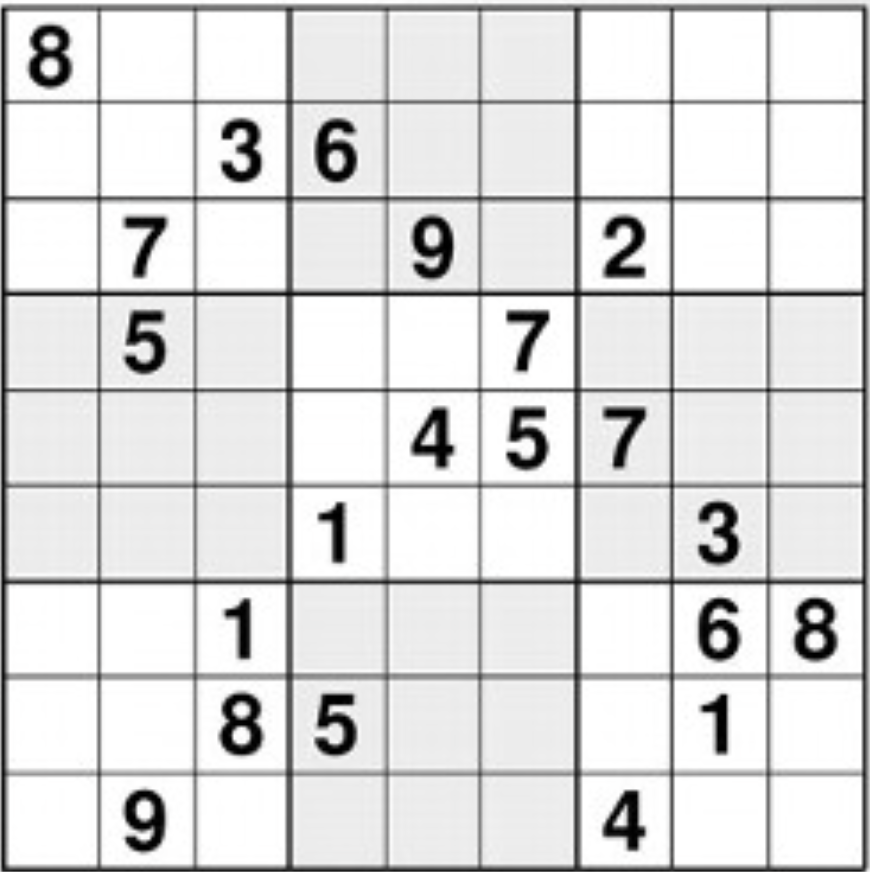
\epsfig{file=Figures/sudoku.png, scale=0.5}} 
  \caption{The Sudoku puzzle created by Arto Inkala.}
  \label{fig:sudoku.png}
\end{figure}

A Sudoku puzzle is a logic-based, combinatorial number-placement puzzle. The objective is to fill a
$9 \times 9$ grid with digits from the set $\{1, \cdots, 9\}$ so that each column, each row, and each of the
nine $3 \times 3$ subgrids that compose the grid (also called "boxes") contain all of these digits exactly
once.  The puzzle is given as a partially completed grid.  A well-posed puzzle must have a single unique
solution.

In order to formulate a Sudoku as a satisfiablity problem from propositional logic, we will use the following
set of propositional variables:
\\[0.2cm]
\hspace*{1.3cm}
$\mathcal{P} = \bigl\{ Q_{r,c,d} \mid r \in \{1,\cdots, 9\} \wedge c \in \{1,\cdots, 9\} \wedge r \in \{1,\cdots, 9\} \bigl\}$
\\[0.2cm]
The variable $Q_{r,c,d}$ is supposed to be \texttt{True} if $d$ is the digit in row $r$ and column $c$ of the
Sudoku.  Note that this means that we have $9^3 = 729$ different propositional variables.  In our
implementation we will use the function \texttt{var} shown in Figure \ref{fig:sudoku-var} to create these variables.

\begin{figure}[!ht]
\centering
\begin{minted}[ frame         = lines, 
                 framesep      = 0.3cm, 
                 firstnumber   = 1,
                 bgcolor       = sepia,
                 numbers       = left,
                 numbersep     = -0.2cm,
                 xleftmargin   = 0.8cm,
                 xrightmargin  = 0.8cm,
               ]{python3}
    def var(row, col, digit):
        return f'Q<{row},{col},{digit}>'
\end{minted}
\vspace*{-0.3cm}
\caption{The function \texttt{var}.}
\label{fig:sudoku-var}
\end{figure}

The Sudoku itself is created by the function \texttt{create\_puzzle} shown in Figure
\ref{fig:sudoku-create-puzzle} on page \pageref{fig:sudoku-create-puzzle}.  In this function, the puzzle is
represented as a list of lists.  Each of these lists represents a row.  The inner lists contain digits and the
characters \texttt{"*"}.  These characters represent the digits that are initially unknown and whose value have
to be computed.

\begin{figure}[!ht]
\centering
\begin{minted}[ frame         = lines, 
                 framesep      = 0.3cm, 
                 firstnumber   = 1,
                 bgcolor       = sepia,
                 numbers       = left,
                 numbersep     = -0.2cm,
                 xleftmargin   = 0.8cm,
                 xrightmargin  = 0.8cm,
               ]{python3}
    def create_puzzle():
        return [ [ 8 , "*", "*", "*", "*", "*", "*", "*", "*"], 
                 ["*", "*",  3 ,  6 , "*", "*", "*", "*", "*"],
                 ["*",  7 , "*", "*",  9 , "*",  2 , "*", "*"],
                 ["*",  5 , "*", "*", "*",  7 , "*", "*", "*"],
                 ["*", "*", "*", "*",  4 ,  5 ,  7 , "*", "*"],
                 ["*", "*", "*",  1 , "*", "*", "*",  3 , "*"],
                 ["*", "*",  1 , "*", "*", "*", "*",  6 ,  8 ],
                 ["*", "*",  8 ,  5 , "*", "*", "*",  1 , "*"],
                 ["*",  9 , "*", "*", "*", "*",  4 , "*", "*"]
               ]
\end{minted}
\vspace*{-0.3cm}
\caption{The function \texttt{create\_puzzle}.}
\label{fig:sudoku-create-puzzle}
\end{figure}

In our implementation we will use functions \texttt{atMostOne} that we have already seen in Figure
\ref{fig:atMostOne} on page \pageref{fig:atMostOne} that expresses that at most one of a given set of
propositional variables is \texttt{True}.  Furthermore, we will use the auxiliary function
$\texttt{atLeastOne}(V)$ which takes a set of propositional variables $V$ and which returns a formula in
conjunctive normal form in set notation that is \texttt{True} if and only if at least one of the variables in
$V$ is \texttt{True}.  Note that in set notation we have
\\[0.2cm]
\hspace*{1.3cm}
$\texttt{atLeastOne}(V) = \bigl\{ V \bigr\}$.
\\[0.2cm]
The reason is that in set notation  $V$ is interpreted as a clause, i.e.~as a disjunction of its variables.
Using these two functions we can then define a function $\texttt{exactlyOne}(V)$ that
takes a set of variables and returns \texttt{True} iff exactly one of the variables in $V$ is \texttt{True}.
The implementation is shown in Figure \ref{fig:sudoku-exactly}.

\begin{figure}[!ht]
\centering
\begin{minted}[ frame         = lines, 
                 framesep      = 0.3cm, 
                 firstnumber   = 1,
                 bgcolor       = sepia,
                 numbers       = left,
                 numbersep     = -0.2cm,
                 xleftmargin   = 0.8cm,
                 xrightmargin  = 0.8cm,
               ]{python3}
    def atLeastOne(S):
        return { frozenset(S) }
    
    def exactlyOne(S):
        return atMostOne(S) | atLeastOne(S)
\end{minted}
\vspace*{-0.3cm}
\caption{The functions \texttt{atLeastOne} and \texttt{exactlyOne}.}
\label{fig:sudoku-exactly}
\end{figure}

Figure \ref{fig:sudoku-exactlyOnce} show the implementation of the function
$\texttt{exactlyOnce}(L)$.  This function takes a set $L$ of pairs as arguments.  Every pair $(r,c) \in L$ is
interpreted as a position in the Sudoku grid whre $r$ specifies the row and $c$ specifies the column of the
position.  The function $\texttt{exactlyOnce}$ computes a set of formulas that express that every digit
$d \in \{1,\cdots,9\}$ occurs exactly once in the set of coordinates $L$: 
\\[0.2cm]
\hspace*{1.3cm}
$\texttt{exactlyOnce}(L) = \bigcup\limits_{d \in \{1,\cdots,9\}} \mathtt{exactlyOne}\bigl(\bigl\{ Q_{r,c,d} \mid (r,c) \in L \bigl\}\bigr)$


\begin{figure}[!ht]
\centering
\begin{minted}[ frame         = lines, 
                 framesep      = 0.3cm, 
                 firstnumber   = 1,
                 bgcolor       = sepia,
                 numbers       = left,
                 numbersep     = -0.2cm,
                 xleftmargin   = 0.8cm,
                 xrightmargin  = 0.8cm,
               ]{python3}
    def exactlyOnce(L):
        Clauses = set()
        for digit in range(1, 10):
            Clauses |= exactlyOne({ var(col, row, digit)  for col, row in L })
        return Clauses
\end{minted}
\vspace*{-0.3cm}
\caption{The function \texttt{exactlyOnce}.}
\label{fig:sudoku-exactlyOnce}
\end{figure}

The function $\texttt{exactlyOneDigit}(r, c)$ takes a row $r$ and a column $c$ as its argument.  It returns a
formula expressing that exactly one of the variables from the set
\\[0.2cm]
\hspace*{1.3cm}
$\bigl\{ Q_{r,c,d} \mid d \in \{1,\cdots, 9\} \bigr\}$
\\[0.2cm]
is \texttt{True}. The implementation is shown in Figure \ref{fig:sudoku-exactlyOneDigit}.

\begin{figure}[!ht]
\centering
\begin{minted}[ frame         = lines, 
                 framesep      = 0.3cm, 
                 firstnumber   = 1,
                 bgcolor       = sepia,
                 numbers       = left,
                 numbersep     = -0.2cm,
                 xleftmargin   = 0.8cm,
                 xrightmargin  = 0.8cm,
               ]{python3}
    def exactlyOneDigit(row, col):
        return exactlyOne({ var(row, col, digit) for digit in range(1, 10) })
\end{minted}
\vspace*{-0.3cm}
\caption{The function \texttt{exactlyOneDigit}.}
\label{fig:sudoku-exactlyOneDigit}
\end{figure}


Furthermore, we need a function encoding the constraints form the puzzle itself.
This function is called \texttt{constraintsFromPuzzle} and its implementation is shown in Figure
\ref{fig:sudoku-constraintsFromPuzzle} on page \pageref{fig:sudoku-constraintsFromPuzzle}.
For example, the given puzzle demands that the digit in row 2 and column 4 is the digit $6$.
This can be expressed as the formula $Q_{2,3,6}$.  In set notation this formula takes the form
\\[0.2cm]
\hspace*{1.3cm}
$\bigl\{ \{Q_{2,3,6}\} \bigr\}$.
\\[0.2cm]
Of course, we have to take the union of all these formula.  This leads to the code shown in Figure
\ref{fig:sudoku-constraintsFromPuzzle} on page \pageref{fig:sudoku-constraintsFromPuzzle}.
Note that we have to provide \texttt{row+1} and \texttt{col+1} as arguments to the function \texttt{var} since
in Python list indices start with $0$.

\begin{figure}[!ht]
\centering
\begin{minted}[ frame         = lines, 
                 framesep      = 0.3cm, 
                 firstnumber   = 1,
                 bgcolor       = sepia,
                 numbers       = left,
                 numbersep     = -0.2cm,
                 xleftmargin   = 0.0cm,
                 xrightmargin  = 0.0cm,
                 ]{python3}
    def constraintsFromPuzzle():
        Puzzle = create_puzzle()
        Variables = [ var(row+1, col+1, Puzzle[row][col]) for row in range(9)
                                                          for col in range(9)
                                                          if  Puzzle[row][col] != '*'
                    ]
        return { frozenset({ var }) for var in Variables }                 
\end{minted}
\vspace*{-0.3cm}
\caption{The function \texttt{constraintsFromPuzzle}}
\label{fig:sudoku-constraintsFromPuzzle}
\end{figure}

Finally, we have to combine all constraints of the puzzle.  This is done with the function \\
\texttt{allConstraints} shown in Figure \ref{fig:sudoku-allConstraints} shown on page \pageref{fig:sudoku-allConstraints}.

\begin{figure}[!ht]
\centering
\begin{minted}[ frame         = lines, 
                 framesep      = 0.3cm, 
                 firstnumber   = 1,
                 bgcolor       = sepia,
                 numbers       = left,
                 numbersep     = -0.2cm,
                 xleftmargin   = 0.8cm,
                 xrightmargin  = 0.8cm,
               ]{python3}
def allConstraints(): 
    L = [1, 2, 3, 4, 5, 6, 7, 8, 9]
    # the constraints from the puzzle have to be satisfied
    Clauses = constraints_from_puzzle()
    # there is exactly one digit in every field
    for row in L:
        for col in L:
            Clauses |= exactlyOneDigit(row, col) 
    # all entries in a row are unique
    for row in L:
        Clauses |= exactlyOnce([ (row, col) for col in L ]) 
    # all entries in a column are unique
    for col in L:
        Clauses |= exactlyOnce([ (row, col) for row in L ])
    # all entries in a 3x3 box are unique    
    for r in range(3):
        for c in range(3):
            S = [ (r * 3 + row, c * 3 + col) for row in range(1, 4)
                                             for col in range(1, 4) 
                ]
            Clauses |= exactlyOnce(S)
    return Clauses
 \end{minted}
\vspace*{-0.3cm}
\caption{The function \texttt{allConstraints}.}
\label{fig:sudoku-allConstraints}
\end{figure}
The Jupyter notebook showing the resulting program is available at:
\\[0.2cm]
\hspace*{1.3cm}
\href{https://github.com/karlstroetmann/Logic/blob/master/Python/Chapter-4/10-Sudoku.ipynb}{\texttt{github.com/karlstroetmann/Logic/blob/master/Python/Chapter-4/10-Sudoku.ipynb}}


\pagebreak

\hspace*{\fill}
\pagebreak

\subsection{PicoSat}
Unfortunately, solving the resulting set of clauses takes about 10 minutes.  Fortunately, there is a version
of the Davis-Putnam algorithm that is implemented in \texttt{C} and that, furthermore, incorporates a number of
improvements to the original algorithm.  This solver is called \href{https://fmv.jku.at/picosat/}{PicoSat}
and has been implemented by \href{https://cca.informatik.uni-freiburg.de/biere/}{Armine Biere}.
A \href{https://github.com/conda/pycosat}{Python API} to this solver is available as
\href{https://pypi.org/project/pycosat/}{pycosat}.  We can install it via \texttt{pip} using the following command:
\\[0.2cm]
\hspace*{1.3cm}
\texttt{pip install pycosat}
\\[0.2cm]
In \textsl{PicoSat} propositional variables are represented as follows:
\begin{enumerate}
\item A propositional variable $p$ is represented as a positive natural number.
\item If $n$ is the natural number representing the propositional variable $p$, then $\neg p$ is represented as
      the integer $-n$. 
\item A clause is represented as a list of integers.
\item A formula in CNF is represented as a list of clauses and hence as a list of list of integers.
\end{enumerate}
For example, if the propositional variables $p$, $q$, and $r$ are represented as the natural numbers
$1$, $2$, and $3$ respectively, then
\begin{enumerate}
\item $p \vee \neg q \vee r$ is represented as the list \texttt{[1, -2, 3]},
\item $\neg p \vee q \vee \neg r$ is represented as the list \texttt{[-1, 2, -3]},
\item $\neg p \vee \neg q \vee r$ is represented as the list \texttt{[-1, -2, 3]}, and
\item $p \vee q \vee \neg r$ is represented as the list \texttt{[1, 2, -3]}.
\end{enumerate}
Finally, the formula 
$$ f = (p \vee \neg q \vee r) \wedge (\neg p \vee q \vee \neg r) \wedge (\neg p \vee \neg q \vee r) \wedge (p \vee q \vee \neg r), $$
which is in conjunctive normal form, is represented as follows:
\\[0.2cm]
\hspace*{1.3cm}
\texttt{f = [ [1, -2, 3], [-1, 2, -3], [-1, -2, 3], [1, 2, -3] ]}
\\[0.2cm]
In order so find a solution to this formula we can call $\texttt{pycosat.solve}(f)$.

\pagebreak
\subsubsection{Transforming Clauses into PyCoSat Format}
In order to use \textsl{PicoSat} to solve the Sudoku discussed earlier, we need a function that transforms a
formula that is in conjunctive normal form into the format of \textsl{PicoSat}.  Furthermore, we need  a function that can translate a solution found by \textsl{PicoSat} back into our format.

The function \texttt{findVariables(Clauses)} in Figure \ref{fig:sudoku-findVariables} on page
\pageref{fig:sudoku-findVariables} takes a set of clauses and returns the set of all propositional variables
occurring in this set.


\begin{figure}[!ht]
\centering
\begin{minted}[ frame         = lines, 
                 framesep      = 0.3cm, 
                 firstnumber   = 1,
                 bgcolor       = sepia,
                 numbers       = left,
                 numbersep     = -0.2cm,
                 xleftmargin   = 0.8cm,
                 xrightmargin  = 0.8cm,
               ]{python3}
    def findVariables(Clauses):
        Variables = set()
        for Clause in Clauses:
            for literal in Clause:
                match literal:
                    case ('¬', var): Variables |= { var }
                    case var       : Variables |= { var }
        return Variables
\end{minted}
\vspace*{-0.3cm}
\caption{The function \texttt{findVariables}.}
\label{fig:sudoku-findVariables}
\end{figure}

The function \texttt{numberVariables(Clauses)} takes a set of clauses as input.  It returns two dictionaries:
\begin{enumerate}
\item The dictionary \texttt{Var2Int} maps every propositional variable occurring in \texttt{Clauses} to a
      unique natural number. 
\item The dictionary \texttt{Int2Var} is the mapping that is inverse to the dictionary \texttt{Var2Int}.
      Hence it maps the natural numbers back to propositional variables.
\end{enumerate}

\begin{figure}[!ht]
\centering
\begin{minted}[ frame         = lines, 
                 framesep      = 0.3cm, 
                 firstnumber   = 1,
                 bgcolor       = sepia,
                 numbers       = left,
                 numbersep     = -0.2cm,
                 xleftmargin   = 0.8cm,
                 xrightmargin  = 0.8cm,
               ]{python3}
    def numberVariables(Clauses):
        Variables = findVariables(Clauses)
        count     = 1
        Var2Int   = {}
        Int2Var   = {}
        for variable in Variables:
            Var2Int[variable] = count
            Int2Var[count   ] = variable
            count += 1
        return Var2Int, Int2Var             
\end{minted}
\vspace*{-0.3cm}
\caption{The function \texttt{numberVariables}}
\label{fig:sudoku-numberVariables}
\end{figure}

\pagebreak
Figure \ref{fig:sudoku-format} shows the remaining auxiliary functions that are necessary to transform a
formula represented as a set of clauses into the format of PicoSat.
\begin{enumerate}
\item The function \texttt{literal2int} takes a literal and transforms this literal into an integer
      representing the literal. If the literal is a negated variable, the integer is negative, else it is
      positive. \texttt{Var2Int} is a dictionary mapping propositional variables to natural numbers.
\item The function \texttt{clause2pyco(Clause, Var2Int)} transforms a set of literals into a list of integers.
      \texttt{Var2Int} is a dictionary mapping the propositional variables to natural numbers. 
\item The function \texttt{clauses2pyco(Clauses, Var2Int)} transforms a set of clauses into a list of lists of
      integers. \texttt{Var2Int} is a dictionary mapping the propositional variables to natural numbers.  
\item The function \texttt{int2var(Numbers, Int2Var)} takes a list of numbers representing a set of literals and returns
      the associated list of literals.  \texttt{Int2Var} is a dictionary mapping natural numbers to
      propositional variables.     
\end{enumerate}

\begin{figure}[!ht]
\centering
\begin{minted}[ frame         = lines, 
                 framesep      = 0.3cm, 
                 firstnumber   = 1,
                 bgcolor       = sepia,
                 numbers       = left,
                 numbersep     = -0.2cm,
                 xleftmargin   = 0.8cm,
                 xrightmargin  = 0.8cm,
               ]{python3}
    def literal2int(literal, Var2Int):
        match literal:
            case ('¬', var): return -Var2Int[var]
            case var       : return  Var2Int[var]
    
    def clause2pyco(Clause, Var2Int):
        return [literal2int(literal, Var2Int) for literal in Clause]
    
    def clauses2pyco(Clauses, Var2Int):
        return [clause2pyco(clause, Var2Int) for clause in Clauses ]
    
    def int2var(Numbers, Int2Var):
        Result = set()
        for n in Numbers:
            if n > 0:
                Result |= {frozenset({Int2Var[n]})}
            else: 
                Result |= {frozenset({ ('¬', Int2Var[-n]) })}
        return Result
\end{minted}
\vspace*{-0.3cm}
\caption{Some axilliary functions to transform clauses into the format of PicoSat.}
\label{fig:sudoku-format}
\end{figure}

The Jupyter notebook showing the resulting program is available at:
\\[0.2cm]
\hspace*{0.3cm}
\href{https://github.com/karlstroetmann/Logic/blob/master/Python/Chapter-4/11-PicoSat-Sudoku.ipynb}{\texttt{github.com/karlstroetmann/Logic/blob/master/Python/Chapter-4/11-PicoSat-Sudoku.ipynb}}

\pagebreak


\section{Check Your Comprehension}
\begin{enumerate}[(a)]
\item How have we defined the set of propositional logic formulas?
\item How have we defined the semantics of propositional logic formulas?
\item How do we represent propositional logic formulas in \textsl{Python}?
\item What is a tautology?
\item How can we transform propositional logic formula into conjunctive normal
      form?
\item Define the notion of an inference rule.
\item when is  an inference rule correct?
\item Define the cut rule.
\item How did we define the proof concept $M \vdash C$?
\item What is a saturated set of clauses?
\item What are the two most important properties of the proof concept $\vdash$?
\item Assume that $M$ is a saturated set of clauses. How can we define a propositional interpretation
      $\mathcal{I}$ such that $\mathcal{I}(C) = \mathtt{True}$ for all $C \in M$?
\item How did we define the notion of a set of clauses being solvable?
\item Do you know how the algorithm of Davis and Putnam works?
\item Can you code a logical puzzle as a propositional formula?
\end{enumerate}


%\input{compact-barwise}

%%% Local Variables: 
%%% mode: latex
%%% TeX-master: "logic"
%%% End: 

\chapter{First-Order Logic}
In \textcolor{blue}{propositional logic}, we have studied the combination of atomic propositions using
the propositional \textcolor{blue}{connectives} ``$\neg$'', ``$\vee$'', ``$\wedge$'', ``$\rightarrow$" and
``$\leftrightarrow$''.  In \blue{first-order logic}\index{first-order logic} we additionally 
examine the structure of these atomic propositions. The following additional concepts are introduced in
first-order logic: 
\begin{enumerate}
\item \textcolor{blue}{Terms} are used as designations for objects.
\item These terms are composed of \textcolor{blue}{object variables} and \textcolor{blue}{function symbols}.
      In the following examples, ``$x$'' is an object variable\index{Object variable}, while
      ``\textsl{father}'' and ``\textsl{mother}'' are unary function symbols\index{function symbol} and
      ``\textsl{isaac}'' is a nullary function symbol:
      \\[0.2cm]
      \hspace*{1.3cm}
      $\textsl{father}(x),\quad \textsl{mother}(\textsl{isaac})$.
      \\[0.2cm]
      Nullary function symbols are also referred to as \textcolor{blue}{constants}\index{constant}
      and instead of object variables we simply talk about variables.
\item Different objects are related by \textcolor{blue}{predicate symbols}\index{Predicate symbols}.
      In the following example, we use the predicate symbols ``\textsl{isBrother}'' and ``$<$''.
      Additionally, ``\textsl{albert}'' and ``\textsl{bruno}'' are constants:
      \\[0.2cm]
      \hspace*{1.3cm}
      $\textsl{isBrother}\bigl(\textsl{albert}, \textsl{father}(\textsl{bruno})\bigr),\quad x+7 < x\cdot 7$.
      \\[0.2cm]
      The resulting formulas are referred to as \textcolor{blue}{atomic formulas} \index{atomic formulas},
      since they do not contain subformulas. 
\item Atomic formulas can be combined using the propositional connectives as shown the following example:
      \\[0.2cm]
      \hspace*{1.3cm}
      $x > 1 \rightarrow x + 7 < x \cdot  7$.
\item Finally, the \textcolor{blue}{quantifiers}\index{quantifiers} ``$\forall$'' (\emph{for all}) and
      ``$\exists$'' (\emph{there exists}) are introduced to distinguish between variables that are
      \textcolor{blue}{existentially} quantified and those variables that are \textcolor{blue}{universally}
      quantified.  For example, the formula 
      \\[0.2cm]
      \hspace*{1.3cm}
      $\forall x \in \mathbb{R}: \exists n \in \mathbb{N}: x < n$
      \\[0.2cm]
      is read as: ``\textsl{For all real numbers $x$ there exists a natural number $n$ such that $x$ is less
        than $n$.}''
\end{enumerate}
This chapter is structured as follows:
\begin{enumerate}[(a)]
\item In the next section, we will define the \href{https://en.wikipedia.org/wiki/Syntax}{syntax} of
      first-order logic formulas, i.e., we will specify those strings that are regarded as first-order
      formulas.
\item In the following section, we deal with the
      \href{https://en.wikipedia.org/wiki/Semantics}{semantics} of these formulas, that is we specify the 
      meaning of first-order formulas.
\item After that, we show how to implement syntax and semantics in \textsl{Python}.
\item As an application of first-order logic we discuss \textcolor{blue}{constraint programming}.
      In constraint programming, a given problem is described using first-order logic formulas.
      To solve the problem, a so-called \textcolor{blue}{constraint solver} is used.
\item We develop a simple constraint solver that works by the means of \blue{backtracking}.
\item Then we discuss the constraint solver \texttt{Z3}, which is a state-of-the-art constraint solver
      developed by Microsoft Corporation.
\item Furthermore, we consider normal forms of first-order logic formulas and show how formulas
      can be transformed into first-order logic clauses.
\item We also discuss a \textcolor{blue}{first-order logic calculus}, which is the basis
      of automatic reasoning in first-order logic.
\item To conclude the chapter, we discuss the automatic theorem prover \textsl{Vampire}.
\end{enumerate}

\section{Syntax of First-Order Logic}
First, we define the concept of a \textcolor{blue}{signature}\index{signature}. Essentially, this is a
structured summary of variables, function symbols, and predicate symbols, along with a specification of the
arity of these symbols. 

\begin{Definition}[Signature]
  A \textcolor{blue}{signature} is a 4-tuple \\[0.2cm]
  \hspace*{1.3cm} $\Sigma = \langle \mathcal{V}, \mathcal{F}, \mathcal{P}, \textsl{arity} \rangle$, \\[0.2cm]
  such that the following holds:
  \begin{enumerate}
  \item $\mathcal{V}$ is the set of \textcolor{blue}{object variables},\index{Object variables} which we often simply refer to as
        \textcolor{blue}{variables} for brevity.
  \item $\mathcal{F}$ is the set of \textcolor{blue}{function symbols}.\index{Function symbols}
  \item $\mathcal{P}$ is the set of \textcolor{blue}{predicate symbols}.\index{Predicate symbols}
  \item $\textsl{arity}$ is a function that assigns each function and predicate symbol its
        \textcolor{blue}{arity}\index{Arity}: \\[0.2cm]
        \hspace*{1.3cm} $\textsl{arity}: \mathcal{F} \cup \mathcal{P} \rightarrow \mathbb{N}$. \\[0.2cm]
        We say that the function or predicate symbol $f$ is an
        $n$-ary symbol if $\textsl{arity}(f) = n$.
        
        A function symbol $c$ such that $\textsl{arity}(c) = 0$ is called a \blue{constant}. \index{constant}
        
        A predicate symbol $p$ such that $\textsl{arity}(p) = 0$ is called a \blue{propositional variable}.
        \index{propositional variable}
  \item Since we need to be able to distinguish between variables, function symbols, and predicate symbols,
        we agree that the sets $\mathcal{V}$, $\mathcal{F}$, and $\mathcal{P}$ have to be pairwise disjoint: \\[0.2cm] 
        \hspace*{1.3cm} $\mathcal{V} \cap \mathcal{F} = \{\}$, \quad
                        $\mathcal{V} \cap \mathcal{P} = \{\}$, \quad and \quad
                        $\mathcal{F} \cap \mathcal{P} = \{\}$. \eox
  \end{enumerate}
\end{Definition}

\exampleEng
Next, we define the signature $\Sigma_G$ of group theory. Let
\begin{enumerate}
\item $\mathcal{V} := \{ x, y, z \}$ be the set of variables,
\item $\mathcal{F} := \{ \mathtt{e}, \circ \}$ be the set of function symbols,
\item $\mathcal{P} := \{\mathtt{=} \}$ be the set of predicate symbols,
\item $\textsl{arity} := \bigl\{ \mathtt{e} \mapsto 0, \mathtt{\circ} \mapsto 2, = \mapsto 2 \bigr\}$
      specifes the arities of function and predicate symbols.
\end{enumerate}
Then the signature $\Sigma_G$ of group theory is defined as follows:
\\[0.2cm]
\hspace*{1.3cm}
$\Sigma_G := \langle \mathcal{V}, \mathcal{F}, \mathcal{P}, \textsl{arity} \rangle$.
\eox
\vspace{0.3cm}

\noindent
We use expressions built from variables and function symbols as identifiers for objects. These expressions are
called \textcolor{blue}{terms}.\index{terms} The formal definition follows.

\begin{Definition}[Terms, $\mathcal{T}_\Sigma$] \hspace*{\fill} \\
  If $\Sigma = \langle \mathcal{V}, \mathcal{F}, \mathcal{P}, \textsl{arity} \rangle$ is a signature, then we
  define the set \textcolor{blue}{$\mathcal{T}_\Sigma$} \index{$\mathcal{T}_\Sigma$}  of
  \textcolor{blue}{$\Sigma$-terms}, 
  inductively:
  \begin{enumerate}
  \item For every variable $x \in \mathcal{V}$, we have that $x \in \mathcal{T}_\Sigma$. Thus, every variable is also a term.
  \item If $c \in \mathcal{F}$ is a $0$-ary function symbol,
        i.e.~$\textsl{arity}(c) = 0$, then $c \in \mathcal{T}_\Sigma$.

        Therefore, every constant is a term.
  \item If $f \in \mathcal{F}$ is an $n$-ary function symbol such that $n > 0$ and 
        $t_1,\cdots,t_n \in \mathcal{T}_\Sigma$, then 
        \\[0.2cm]
        \hspace*{1.3cm} $f(t_1,\cdots,t_n) \in \mathcal{T}_\Sigma$,
        \\[0.2cm]
        thus the expression $f(t_1,\cdots,t_n) \in \mathcal{T}_\Sigma$ is a term.
        \eox
  \end{enumerate}
\end{Definition}

\exampleEng
Let
\begin{enumerate}
\item $\mathcal{V} := \{ x, y, z \}$ be the set of variables,
\item $\mathcal{F} := \{ 0, 1, \mathtt{+}, \mathtt{-}, * \}$ be the set of function symbols,
\item $\mathcal{P} := \{\mathtt{=}, \leq\}$ be the set of predicate symbols,
\item $\textsl{arity} := \bigl\{ 0 \mapsto 0, 1 \mapsto 0, \mathtt{+} \mapsto 2, \mathtt{-} \mapsto 2,
                                 * \mapsto 2, = \mapsto 2, \leq \mapsto 2 \bigr\}$
      specify the arity of function and predicate symbols, and
\item $\Sigma_\mathrm{arith} := \langle \mathcal{V}, \mathcal{F}, \mathcal{P}, \textsl{arity} \rangle$
      be a signature.
\end{enumerate}
Then we can construct $\Sigma_{\mathrm{arith}}$-terms as follows:
\begin{enumerate}
\item $x, y, z \in \mathcal{T}_{\Sigma_{\mathrm{arith}}}$, \\[0.2cm]
      since all variables are also $\Sigma_{\mathrm{arith}}$-terms.
\item $0, 1 \in \mathcal{T}_{\Sigma_{\mathrm{arith}}}$,  \\[0.2cm]
      since $0$ and $1$ are nullary function symbols.
\item $\mathtt{+}(0,x) \in \mathcal{T}_{\Sigma_{\mathrm{arith}}}$, \\[0.2cm]
      since $0 \in \mathcal{T}_{\Sigma_{\mathrm{arith}}}$, $x \in \mathcal{T}_{\Sigma_{\mathrm{arith}}}$ and 
      $\mathtt{+}$ is a binary function symbol.
\item $*(\mathtt{+}(0,x),1) \in \mathcal{T}_{\Sigma_{\mathrm{arith}}}$, \\[0.2cm]
      since $\mathtt{+}(0,x) \in \mathcal{T}_{\Sigma_{\mathrm{arith}}}$, $1 \in \mathcal{T}_{\Sigma_{\mathrm{arith}}}$ and
      $*$ is a binary function symbol.
\end{enumerate}
In practice, for certain binary functions, we use an \textcolor{blue}{infix notation},
i.e., we write binary function symbols between their arguments. For example,
we write $x+y$ instead of $+(x,y)$. The infix notation is then to be understood as an abbreviation for the
above-defined representation. This, of course, works only if we also set precedence levels for the various operators.
\eox

Next, we define the concept of \textcolor{blue}{atomic formulas}.\index{Atomic Formulas} These are formulas
that cannot be decomposed into smaller formulas: atomic formulas thus contain neither propositional connectives
nor quantifiers. 
\begin{Definition}[Atomic Formulas, $\mathcal{A}_\Sigma$]
  Given a signature $\Sigma = \langle \mathcal{V}, \mathcal{F}, \mathcal{P}, \textsl{arity} \rangle$. 
  The set of atomic $\Sigma$-formulas $\mathcal{A}_\Sigma$ \index{$\mathcal{A}_\Sigma$}
  is defined as follows:
  \begin{enumerate}
  \item $\verum \in \mathcal{A}_\Sigma$ and  $\falsum \in \mathcal{A}_\Sigma$.
  \item If $p \in \mathcal{P}$ and $\textsl{arity}(p)= 0$, then $p \in \mathcal{A}_\Sigma$.

        Therefore, propositional variables are atomic formulas.
  \item If $p \in \mathcal{P}$ is an $n$-ary predicate symbol such that $n > 0$ and, furthermore,  $n$ $\Sigma$-terms
        $t_1$, $\cdots$, $t_n$ are given, then  $p(t_1,\cdots,t_n)$ is an \textcolor{blue}{atomic $\Sigma$-formula}: \\[0.2cm]
        \hspace*{1.3cm} $p(t_1,\cdots,t_n) \in \mathcal{A}_\Sigma$.  \qed
  \end{enumerate}
\end{Definition}

\exampleEng
Continuing from the last example, we can see that \\[0.2cm]
\hspace*{1.3cm} $\mathtt{=}(*(\mathtt{+}(0,x),1),0)$ \\[0.2cm]
is an atomic $\Sigma_\mathrm{arith}$-formula. Note that we have not yet discussed the truth value of such
formulas. The question of whether a formula is considered true or false
will be explored in the next section.

In practice we will often use infix notation for binary predicate symbols.  The atomic formula given above is then
written as
\\[0.2cm]
\hspace*{1.3cm}
$(0 + x) * 1 = 0$.
\eox


\subsection{Bound Variables and Free Variables}
In defining first-order logic formulas, it is necessary
to distinguish between so-called \textcolor{blue}{bound}\index{bound variable} and \textcolor{blue}{free}
variables\index{free variable}.
We introduce these concepts informally using an example from calculus.
Consider the following equation: \\[0.2cm]
\hspace*{1.3cm}
$\ds\int_{0}^{x} y \cdot t\, dt = \frac{1}{2} \cdot x^2 \cdot y$
\\[0.2cm]
In this equation, the variables $x$ and $y$ occur \textcolor{blue}{free}, while the variable $t$ is \textcolor{blue}{bound} by the integral.
This means the following: We can substitute arbitrary values for $x$ and $y$ in this equation without
changing the validity of the formula. For example, substituting $2$ for $x$, we get \\[0.2cm]
\hspace*{1.3cm}
$\ds\int_{0}^{2} y \cdot t\, dt = \frac{1}{2} \cdot 2^2 \cdot y$ \\[0.2cm]
and this equation is also valid. Conversely, it makes no sense to substitute a number for the bound variable
$t$.
The left side of the resulting equation would simply be undefined. We can only replace $t$
with another variable.
For example, replacing variable $t$ with $u$, we get \\[0.2cm]
\hspace*{1.3cm}
$\ds\int_{0}^{x} y \cdot u\, du = \frac{1}{2} \cdot x^2 \cdot y$
\\[0.2cm]
and this is effectively the same statement as above. However, this does not work with every variable. If we
substitute the variable $y$ for $t$, we get \\[0.2cm]
\hspace*{1.3cm}
$\ds\int_{0}^{x} y \cdot y\, dy = \frac{1}{2} \cdot x^2 \cdot y$. \\[0.2cm]
This statement is incorrect! The problem is that the previously free variable
$y$ becomes bound during the substitution.

A similar problem arises when we substitute arbitrary terms for $y$. As long as these terms do not contain the variable $t$,
everything is fine. For example, if we substitute the term $x^2$ for $y$, we get \\[0.2cm]
\hspace*{1.3cm}
$\ds\int_{0}^{x} x^2 \cdot t\, dt = \frac{1}{2} \cdot x^2 \cdot x^2$
\\[0.2cm]
and this formula is valid. However, if we substitute the term $t^2$ for $y$, we get \\[0.2cm]
\hspace*{1.3cm}
$\ds\int_{0}^{x} t^2 \cdot t\, dt = \frac{1}{2} \cdot x^2 \cdot t^2$
\\[0.2cm]
and this formula is no longer valid.  These examples show that we have to distinguish between bound and free
variables. 

In first-order logic, the quantifiers ``$\forall$'' (\textcolor{blue}{for all}) and ``$\exists$''
(\textcolor{blue}{there exists}) bind variables in a similar way as the integral operator
``$\int \cdot\; \mathtt{d}t$''. The above explanations show that there are two different types of 
variables: \textcolor{blue}{free variables} and \textcolor{blue}{bound variables}.
To clarify these concepts, we first define for a
$\Sigma$-term $t$ the set of variables contained in $t$.

\begin{Definition}[$\var(t)$]
  \index{$\var(t)$}
  Given a signature $\Sigma = \langle \mathcal{V}, \mathcal{F}, \mathcal{P}, \textsl{arity} \rangle$ and
  $t$ a $\Sigma$-term, we define the set \textcolor{blue}{$\var(t)$} of variables that occur in $t$
  by induction on the structure of the term:
  \begin{enumerate}
    \item $\var(x) := \{ x \}$ \quad for all $x \in \mathcal{V}$,
    \item $\var(c) := \{ \}$ \quad for all $c \in \mathcal{F}$ such that $\textsl{arity}(c) = 0$,
    \item $\var\bigl(f(t_1,\cdots,t_n)\bigr) := \var(t_1) \cup \cdots \cup \var(t_n)$.
          \eox
  \end{enumerate}
\end{Definition}

\subsection{$\Sigma$-Formulas}
\begin{Definition}[$\Sigma$-Formula, $\mathbb{F}_\Sigma$, bound and free variables, $\textsl{BV}(F)$, $\textsl{FV}(F)$]
\label{predicate-formula} \hspace*{\fill}
\index{$\Sigma$-Formula} \index{$\mathbb{F}_\Sigma$}\index{bound variables}\index{free
  variables}\index{$\textsl{BV}(F)$}\index{$\textsl{FV}(F)$} \\
Let $\Sigma = \langle \mathcal{V}, \mathcal{F}, \mathcal{P}, \textsl{arity} \rangle$ be a signature.
    We denote the set of \textcolor{blue}{$\Sigma$-\emph{Formulas}} by $\mathbb{F}_\Sigma$.
    We define this set inductively.
    Simultaneously, for each formula $F \in \mathbb{F}_\Sigma$, we define the set $\textsl{BV}(F)$ of variables
    that occur \textcolor{blue}{bound} in $F$ and the set $\textsl{FV}(F)$ of variables that occur
    \textcolor{blue}{free} in $F$. 
    \begin{enumerate}
    \item $\falsum \in \mathbb{F}_\Sigma$ and $\verum \in \mathbb{F}_\Sigma$, and we define \\[0.2cm]
          \hspace*{1.3cm} $\FV(\falsum) := \FV(\verum) := \BV(\falsum) := \BV(\verum) := \{\}$.
    \item If $p \in \mathcal{A}_\Sigma$ and $\textsl{arity}(p)= 0$, then $p \in \mathbb{F}_\Sigma$ and    
          \\[0.2cm]
          \hspace*{1.3cm}
          \hspace*{1.3cm} $\FV(p) := \{\}$ \quad and \quad $\BV(p) := \{\}$.
    \item If $F = p(t_1,\cdots,t_n)$ is an atomic $\Sigma$-formula, then $F \in \mathbb{F}_\Sigma$.
          Furthermore, we have
          \begin{enumerate}
          \item $\FV\bigl(p(t_1,\cdots,t_n) \bigr) := \var(t_1) \cup \cdots \cup \var(t_n)$,
          \item $\BV\bigl(p(t_1,\cdots,t_n) \bigr) := \{\}$.
          \end{enumerate}
    \item If $F \in \mathbb{F}_\Sigma$, then $\neg F \in \mathbb{F}_\Sigma$.  Furthermore, we have
          \begin{enumerate}
          \item $\FV\bigl( \neg F \bigr) := \FV(F)$,
          \item $\BV\bigl( \neg F \bigr) := \BV(F)$.
          \end{enumerate}
    \item If $F, G \in \mathbb{F}_\Sigma$ and additionally \\[0.2cm]
          \hspace*{1.3cm}
          $\bigl(\FV(F) \cup \FV(G)\bigr) \cap \bigl(\BV(F) \cup \BV(G)) = \{\}$,
          \\[0.2cm]
          then it also holds that
          \begin{enumerate}
          \item $(F \wedge G) \in \mathbb{F}_\Sigma$,
          \item $(F \vee G) \in \mathbb{F}_\Sigma$,
          \item $(F \rightarrow G) \in \mathbb{F}_\Sigma$,
          \item $(F \leftrightarrow G) \in \mathbb{F}_\Sigma$.
          \end{enumerate}
          Furthermore, we define for all propositional connectives $\odot \in \{ \wedge, \vee, \rightarrow, \leftrightarrow \}$:
          \begin{enumerate}
          \item $\FV\bigl((F \odot G) \bigr) := \FV(F) \cup \FV(G)$.
          \item $\BV\bigl((F \odot G) \bigr) := \BV(F) \cup \BV(G)$.
          \end{enumerate}
    \item Let $x \in \mathcal{V}$ and $F \in \mathbb{F}_\Sigma$ with $x \not\in \BV(F)$. Then:
          \begin{enumerate}
          \item $(\forall x : F) \in \mathbb{F}_\Sigma$,
          \item $(\exists x : F) \in \mathbb{F}_\Sigma$.
          \end{enumerate}
          Furthermore, we define
          \begin{enumerate}
          \item $\FV\bigl( (\forall x : F) \bigr) := \FV\bigl( (\exists x : F) \bigr) := \FV(F) \backslash \{x\}$,
          \item $\BV\bigl( (\forall x : F) \bigr) := \BV\bigl( (\exists x : F) \bigr) := \BV(F) \cup \{x\}$.  
          \end{enumerate}
    \end{enumerate}
    If the signature $\Sigma$ is clear from the context or irrelevant, we may also write
    $\mathbb{F}$ instead of $\mathbb{F}_\Sigma$ and simply refer to formulas instead of $\Sigma$-formulas.
    \eox
\end{Definition}

In the definition given above, we have taken care that a variable cannot appear both free and bound in a
formula simultaneously, because a straightforward induction on the structure of the formulas shows that for all 
$F \in \mathbb{F}_\Sigma$ the following holds:  
\\[0.2cm]
\hspace*{1.3cm}
$ \FV(F) \cap \BV(F) = \{\}$. 

\exampleEng
Continuing the example started above, we see that \\[0.2cm]
\hspace*{1.3cm} $(\exists x \colon\, \leq\!(\mathtt{+}(y, x),y))$ \\[0.2cm]
is a formula from $\mathbb{F}_{\Sigma_{\mathrm{arith}}}$. 
The set of bound variables is $\{x\}$, the set of free variables is 
$\{ y \}$. \eox

If we would always write formulas in the prefix notation defined above, then readability would suffer
disproportionately.  
To abbreviate, we agree that in first-order logic the same rules for saving parentheses apply that we have
already used in propositional logic. In addition, the same quantifiers are combined: for example, we write   
\\[0.2cm]
\hspace*{1.3cm}
$\forall x, y \colon p(x, y)  \quad \text{instead of} \quad \forall x \colon ( \forall y \colon p(x,y))$.
\\[0.2cm]
Moreover, we agree that we may also indicate binary predicate and function symbols in infix notation.
In order to guarantee a unique readability, we must then define the precedence and the associativity of the
function symbols.  For example, we write \\[0.2cm]
\hspace*{1.3cm} $\mathtt{n}_1 = \mathtt{n}_2$  \quad instead of \quad $=(\mathtt{n}_1, \mathtt{n}_2)$. \\[0.2cm]
The formula $(\exists x \colon \leq(\mathtt{+}(y, x),y))$ becomes more readable as \\[0.2cm]
\hspace*{1.3cm} $\exists x \colon y + x \leq y$ \\[0.2cm]
Moreover, in the literature, you will often find expressions of the form
\\[0.2cm]
\hspace*{1.3cm}
$\forall x \in M: F$ \quad or \quad $\exists x \in M: F$.
\\[0.2cm]
These are abbreviations defined as
\\[0.2cm]
\hspace*{1.3cm}
$\ds \bigl(\forall x \in M: F\bigr) \stackrel{\mathrm{def}}{\Longleftrightarrow} \forall x: \bigl(x \in M \rightarrow F\bigr)$
\quad and \quad 
$\ds\bigl(\exists x \in M: F\bigr) \stackrel{\mathrm{def}}{\Longleftrightarrow} \exists x: \bigl(x \in M \wedge F\bigr)$.
\\[0.2cm]
Finally, we agree that quantifiers bind more tightly than the operators $\wedge$, $\vee$, $\rightarrow$, and
$\leftrightarrow$. 

\exerciseEng
\noindent \textbf{Consider the following signature for formalizing family relationships:}
\begin{itemize}
    \item \textbf{Variables:} $\{ u, v, w, x, y, z \}$.
    \item \textbf{Function Symbols:}
    \begin{itemize}
        \item $\texttt{mother}(x)$: the mother of $x$.
        \item $\texttt{father}(x)$: the father of $x$.
    \end{itemize}
    \item \textbf{Unary Predicates:}
    \begin{itemize}
        \item $\texttt{female}(x)$: $x$ is female.
        \item $\texttt{male}(x)$: $x$ is male.
    \end{itemize}
    \item \textbf{Binary Predicates:}
    \begin{itemize}
    \item $\texttt{brother}(x,y)$: $x$ is a brother of $y$.
    \item $\texttt{sister}(x,y)$: $x$ is a sister of $y$.
    \item $\texttt{sibling}(x,y)$: $x$ is a sibling of $y$.
    \item $\texttt{married}(x,y)$: $x$ is married to $y$.
    \item $\texttt{grandmother}(x,y)$: $x$ is a grandmother of $y$.
    \item $\texttt{grandfather}(x,y)$: $x$ is a grandfather of $y$.
    \item $\texttt{grandchild}(x, y)$: $x$ is a grandchild of $y$,
    \item $\texttt{uncle}(x,y)$: $x$ is an uncle of $y$.
    \item $\texttt{aunt}(x,y)$: $x$ is an aunt of $y$.
    \item $\texttt{cousin}(x,y)$: $x$ is a cousin of $y$.
    \end{itemize}
\end{itemize}
In the following, your task is to \blue{define} certain predicates. In general, a \blue{definition} of an
$n$-ary predicate $p$ has the form 
\\[0.2cm]
\hspace*{1.3cm}
$\forall x_1, \cdots, x_n: \bigl(p(x_1,\cdots,x_n) \leftrightarrow F\bigr)$,
\\[0.2cm]
where $F$ is a formula that does not contain the predicate $p$.  In this exercise, this formula
may only contain the function symbols \texttt{mother} and \texttt{father} and the predicate symbols \texttt{male} and
\texttt{female}.  For the purpose of this exercise we make the simplifying assumption that
every person is either femal or male.

As an example, to \texttt{define} the predicate \texttt{brother} we can use the following formula:
\\[0.2cm]
\hspace*{1.3cm}
$\forall x, y:\bigl(\mathtt{brother}(x, y) \leftrightarrow \mathtt{male}(x) \wedge \mathtt{father}(x)
= \mathtt{father}(y) \wedge \mathtt{mother}(x) = \mathtt{mother}(y)\bigr)$
\\[0.2cm]
Define the following predicates:
\begin{enumerate}[(a)]
\item $\texttt{sister}(x, y)$,
\item $\texttt{aunt}(x, y)$,
\item $\mathtt{uncle}$,
\item $\texttt{sibling}(x, y)$,
\item $\texttt{grandfather}(x, y)$,
\item $\texttt{grandmother}(x, y)$,
\item $\texttt{grandchild}(x, y)$,
\item $\texttt{cousin}(x, y)$.
  \eox
\end{enumerate}


\section{Semantics of First-Order Logic \label{sec:semantik}}
Next, we define the \blue{meaning} of the formulas. For this purpose, we introduce the concept of a
\blue{$\Sigma$-structure}. \index{$\Sigma$-structure} This kind of structure specifies how the
function and predicate symbols of the signature $\Sigma$ are to be interpreted.

\begin{Definition}[Structure]
    Let a signature \\[0.2cm]
    \hspace*{1.3cm} $\Sigma = \langle \mathcal{V}, \mathcal{F}, \mathcal{P}, \textsl{arity} \rangle$ \\[0.2cm]
    be given. A \blue{$\Sigma$-structure} $\struct$ is a
    pair $\langle \mathcal{U}, \mathcal{J} \rangle$, such that the following holds:
    \begin{enumerate}
        \item $\mathcal{U}$ is a non-empty set. This set is also called the
              \blue{universe} \index{universe} of the $\Sigma$-structure. This universe contains the values,
              which will later result from the evaluation of terms.
        \item $\mathcal{J}$ is the \blue{interpretation} \index{interpretation} of the function and predicate symbols.
              Formally, we define $\mathcal{J}$ as a mapping with the following properties:
        \begin{enumerate}
        \item Every function symbol $c \in \mathcal{F}$ with $\textsl{arity}(f) = 0$ is mapped to an element
              of $\mathcal{U}$, i.e.~we have $\mathcal{J}(c) \in \mathcal{U}$.  Instead of writing
              $\mathcal{J}(c)$ we will write $c^{\mathcal{J}}$.
        \item Every function symbol $f \in \mathcal{F}$ with $\textsl{arity}(f) = m$ and $m > 0$ is mapped to
              an $m$-ary function \\[0.2cm]
              \hspace*{1.3cm}
              $f^\mathcal{J}\colon \mathcal{U}^m \rightarrow \mathcal{U}$ \\[0.2cm]
              that maps $m$-tuples of the universe $\mathcal{U}$ into the universe $\mathcal{U}$.
        \item Every predicate symbol $p \in \mathcal{P}$ with $\textsl{arity}(p) = 0$ is mapped to
              the set $\mathbb{B}$ of truth values, i.e.~$p^{\mathcal{J}} \in \{ \mathtt{True}, \mathtt{False}\}$.
        \item Every predicate symbol $p \in \mathcal{P}$ with $\textsl{arity}(p) = n$ such that $n > 0$ is mapped to
              a subset \\[0.2cm]
              \hspace*{1.3cm} 
              $p^\mathcal{J} \subseteq \mathcal{U}^n$. \\[0.2cm]
              The idea is that an atomic formula of the form $p(t_1, \cdots, t_n)$
              is interpreted as $\texttt{True}$ exactly if the interpretation of the tuple
              $\langle t_1, \cdots, t_n \rangle$ is an element of the set $p^\mathcal{J}$.
        \item If the symbol ``$=$'' is a member of the set of predicate symbols $\mathcal{P}$, then the
              interpretation of  the equality symbol ``$=$'' has to be \blue{canonical}, i.e.~we must have
              \\[0.2cm]
              \hspace*{1.3cm}  
              $=^\mathcal{J} \;=\; \bigl\{ \langle u, u \rangle \mid u \in \mathcal{U} \bigr\}$.
              \\[0.2cm]
              A formula of the type $s = t$ is thus interpreted as true 
              exactly when the interpretation of the term $s$ yields the same value as the interpretation of
              the term $t$. 
              \eox
        \end{enumerate}
    \end{enumerate}
\end{Definition}

\exampleEng
The signature $\Sigma_G$ of group theory is defined as \\[0.2cm]
\hspace*{1.3cm} $\Sigma_G = \langle \mathcal{V}, \mathcal{F}, \mathcal{P},\textsl{arity}\rangle$ 
\quad with
\begin{enumerate}
\item $\mathcal{V} := \{ x, y, z \}$
\item $\mathcal{F} := \{ \mathrm{e}, * \}$
\item $\mathcal{P} := \{ \mathtt{=} \}$
\item $\textsl{arity} = \bigl\{ \pair(\mathrm{e},0), \pair(*,2), \pair(\mathtt{=},2)\bigr\}$
\end{enumerate}
We can then define a $\Sigma_G$ structure $\mathcal{Z} = \langle \{0,1\},\mathcal{J}\rangle$ 
by defining the interpretation $\mathcal{J}$ 
as follows:
\begin{enumerate}
\item $\mathrm{e}^\mathcal{J} := 0$,
\item $*^\mathcal{J} := \Bigl\{ \pair(0,0) \mapsto 0,\;
                                 \pair(0,1) \mapsto 1,\;
                                 \pair(1,0) \mapsto 1,\;
                                 \pair(1,1) \mapsto 0 \Bigr\}$,
\item $=^\mathcal{J} \;:=\; \bigl\{ \pair(0,0), \pair(1,1) \bigr\}$.
                                 
      Note that we have no leeway in the interpretation of the equality symbol! \eox
\end{enumerate}

If we want to evaluate terms that contain variables, we have to substitute values from the universe 
for these variables. Which values we substitute is determined by a \blue{variable
  assignment}\index{variable assignment}.  We define this concept next. 

\begin{Definition}[Variable Assignment]
    Assume a signature \\[0.2cm]
    \hspace*{1.3cm} $\Sigma = \langle \mathcal{V}, \mathcal{F}, \mathcal{P}, \textsl{arity} \rangle$ \\[0.2cm]
    is given.  Furthermore,  $\struct = \langle \mathcal{U}, \mathcal{J} \rangle$ is a  $\Sigma$-structure.
    Then a function of the form \\[0.2cm]
    \hspace*{1.3cm} $\mathcal{I}: \mathcal{V} \rightarrow \mathcal{U}$ \\[0.2cm]
    is called an {\color{blue}$\struct$ \emph{variable assignment}}.

    If  $\mathcal{I}$ is an $\struct$ variable assignment, 
    $x \in \mathcal{V}$ and $c \in \mathcal{U}$, then \blue{$\mathcal{I}[x/c]$} denotes the variable assignment
    that maps the variable  $x$ to the value $c$ and that otherwise agrees with $\mathcal{I}$: \\[0.2cm]
    \hspace*{1.3cm} 
    $\mathcal{I}[x/c](y) := \left\{
    \begin{array}{ll}
    c               & \mbox{if}\; y = x;  \\
    \mathcal{I}(y)  & \mbox{otherwise}.          \\
    \end{array}
    \right.$ \eox
\end{Definition}


\begin{Definition}[Interpretation of Terms]
  If $\Sigma = \langle \mathcal{V}, \mathcal{F}, \mathcal{P}, \textsl{arity} \rangle$ is a signature
  $\struct = \pair(\mathcal{U},\mathcal{J})$ is a  $\Sigma$-structure and $\mathcal{I}$ is an  $\struct$
    variable assignment, then for every term $t$ the \blue{value} \blue{$\struct(\mathcal{I}, t)$}
    \index{$\struct(\mathcal{I}, t)$} is defined by induction on $t$:
    \begin{enumerate}
    \item If $x \in \mathcal{V}$ we define: \\[0.2cm]
          \hspace*{1.3cm} $\struct(\mathcal{I}, x) := \mathcal{I}(x)$.
    \item If $c \in \mathcal{F}$ and $\textsl{arity}(c) = 0$, then $\mathcal{S}(\mathcal{I}, c) := c^\mathcal{J}$.
    \item If $t$ is a term of the form $f(t_1,\cdots,t_n)$, then we define \\[0.2cm]
          \hspace*{1.3cm} $\struct\bigl(\mathcal{I}, f(t_1,\cdots,t_n)\bigr) := 
                           f^\mathcal{J}\bigl( \struct(\mathcal{I}, t_1), \cdots, \struct(\mathcal{I}, t_n) \bigr)$.
                           \eox
    \end{enumerate}
\end{Definition}

\exampleEng
Given the $\Sigma_G$-structure
$\mathcal{Z}$ we define a $\mathcal{Z}$ variable assignment $\mathcal{I}$ as follows:
\\[0.2cm]
\hspace*{1.3cm} $\mathcal{I} := \bigl\{ x \mapsto 0,\; y \mapsto 1,\; z \mapsto 0\bigr\}$.
\\[0.2cm]
The previous line is interpreted as follows:
\\[0.2cm]
\hspace*{1.3cm} $\mathcal{I}(\mathtt{x}) := 0$, \quad $\mathcal{I}(\mathtt{y}) := 1$, \quad and \quad $\mathcal{I}(\mathtt{z}) := 0$.
\\[0.2cm]
Then we have  \\[0.2cm]
\hspace*{1.3cm}  $\mathcal{Z}\bigl(\mathcal{I}, \mathtt{x} * \mathtt{y} \bigr) = 1$. \eox



\exampleEng
If we continue our previous example we have
\\[0.2cm]
\hspace*{1.3cm} 
$\mathcal{Z}(\mathcal{I},x * y = y * x) = \mathtt{True}$.
\eox

To define the semantics of arbitrary $\Sigma$-formulas, we assume that we have the following functions
available, just like in propositional logic: 
\begin{enumerate}
\item $\circneg: \mathbb{B} \rightarrow \mathbb{B}$,
\item $\circvee: \mathbb{B} \times \mathbb{B} \rightarrow \mathbb{B}$,
\item $\circwedge: \mathbb{B} \times \mathbb{B} \rightarrow \mathbb{B}$,
\item $\circright: \mathbb{B} \times \mathbb{B} \rightarrow \mathbb{B}$,
\item $\circleftright: \mathbb{B} \times \mathbb{B} \rightarrow \mathbb{B}$.
\end{enumerate}
The definitions of these functions have been given by the table in Figure \ref{tab:aussagen-logik} on page
\pageref{tab:aussagen-logik}.

\begin{Definition}[Semantics of $\Sigma$-formulas]
    Let $\struct = \langle \mathcal{U}, \mathcal{J} \rangle$ be a $\Sigma$-structure and $\mathcal{I}$ a $\struct$-variable assignment.  
    For each $\Sigma$-formula $F$ the value \blue{$\struct(\mathcal{I},F)$} is defined
    by induction:
    \begin{enumerate}
    \item $\struct(\mathcal{I},\verum) := \mathtt{True}$ and $\struct(\mathcal{I},\falsum) := \mathtt{False}$.
    \item If $p$ is a propositional variable, then we define the value of $p$ as follows:
          \\[0.2cm]
          \hspace*{1.3cm}
          $\mathcal{S}(\mathcal{I}, p) := p^\mathcal{J}$.
    \item For each atomic $\Sigma$-formula of the form $p(t_1, \cdots, t_n)$ we define the value  as follows: \\[0.2cm]
          \hspace*{1.3cm}
          $\struct\bigl(\mathcal{I}, p(t_1,\cdots,t_n)\bigr) := 
          \Bigl(\bigl\langle \struct(\mathcal{I}, t_1), \cdots, \struct(\mathcal{I}, t_n) \bigr\rangle \in p^\mathcal{J}\Bigr)$.
    \item $\struct(\mathcal{I}, \neg F) := \circneg\bigl(\struct(\mathcal{I}, F)\bigr)$.
    \item $\struct(\mathcal{I}, F \wedge G) := \circwedge\bigl(\struct(\mathcal{I}, F), \struct(\mathcal{I}, G)\bigr)$.
    \item $\struct(\mathcal{I}, F \vee G) := \circvee\bigl(\struct(\mathcal{I}, F), \struct(\mathcal{I}, G)\bigr)$.
    \item $\struct(\mathcal{I}, F \rightarrow G) := \circright\bigl(\struct(\mathcal{I}, F), \struct(\mathcal{I}, G)\bigr)$.
    \item $\struct(\mathcal{I}, F \leftrightarrow G) := \circleftright\bigl(\struct(\mathcal{I}, F), \struct(\mathcal{I}, G)\bigr)$.
    \item $\struct\bigl(\mathcal{I}, \forall x\colon F\bigr) := \left\{
      \begin{array}{ll}
         \mathtt{True}  & \mbox{if}\; \struct(\mathcal{I}[x/c], F) = \mathtt{True}\quad \mbox{for all}\; c\in \mathcal{U}\;\mbox{holds}; \\
         \mathtt{False} & \mbox{otherwise}.
      \end{array}
      \right.$
    \item $\struct\bigl(\mathcal{I}, \exists x \colon F\bigr) := \left\{
      \begin{array}{ll}
         \mathtt{True}  & \mbox{if}\; \struct(\mathcal{I}[x/c], F) = \mathtt{True}\quad \mbox{for some}\; c\in \mathcal{U}\;\mbox{holds}; \\
         \mathtt{False} & \mbox{otherwise}.
      \end{array}
      \right.$\eox    
    \end{enumerate}
\end{Definition}

\exampleEng
Continuing from the above example, we have \\[0.2cm]
\hspace*{1.3cm}  $\mathcal{Z}\bigl(\mathcal{I}, \forall \mathtt{x}: \mathrm{e} * x = x \bigr) = \mathtt{True}$.
\eox

\begin{Definition}[Universally valid] \index{Universally valid}
    If $F$ is a $\Sigma$-formula such that for every $\Sigma$-structure $\struct$ and for every
    $\struct$-variable assignment $\mathcal{I}$ \\[0.2cm]
    \hspace*{1.3cm} $\struct(\mathcal{I}, F) = \mathtt{True}$ \\[0.2cm]
    holds, we call $F$ \blue{universally valid}. In this case, we write \\[0.2cm]
    \hspace*{1.3cm} $\models F$. 
    \eox
\end{Definition}

If $F$ is a formula such that $\FV(F) = \{\}$, then the value $\struct(\mathcal{I}, F)$ 
obviously does not depend on the interpretation $\mathcal{I}$. We also refer to such formulas as 
\blue{closed} formulas.\index{closed formula} In this case, we write $\struct(F)$
instead of $\struct(\mathcal{I}, F)$. If additionally $\struct(F) = \mathtt{True}$, 
we also say that $\struct$ is a \blue{model} \index{model} of $F$.
This is written as \\[0.2cm]
\hspace*{1.3cm} $\mathcal{S} \models F$. \index{$\mathcal{S} \models F$}
\vspace{0.1cm}

The definitions of the terms ``\blue{satisfiable}'' and
``\blue{equivalent}'' can now be transferred from propositional logic. 
To avoid unnecessary complexity in the definitions, we assume a
fixed signature $\Sigma$ as given. Hence, in the following definitions
when we talk about terms, formulas, structures, etc., we mean $\Sigma$-terms,
$\Sigma$-formulas, and $\Sigma$-structures.

\begin{Definition}[Equivalent] \index{equivalent}
  Two formulas $F$ and $G$, in which the variables $x_1$, $\cdots$, $x_n$ appear free, are called
  \blue{equivalent} if and only if  
  \\[0.2cm] 
  \hspace*{1.3cm}
  $\models \forall x_1: \cdots\, \forall x_n: (F \leftrightarrow G)$
  \\[0.2cm] 
  holds. If no variables appear free in $F$ and $G$, then $F$ is equivalent to $G$ if and only if
  \\[0.2cm]
  \hspace*{1.3cm}
  $\models F \leftrightarrow G$
  \\[0.2cm]
  holds.  If $F$ and $G$ are equivalent, then this will be written as
  \\[0.2cm]
  \hspace*{1.3cm}
  $F \;\Leftrightarrow\; G$.
  \eox
\end{Definition}

\remarkEng
All propositional logic equivalences are also first-order logic equivalences.
\eox

\begin{Definition}[Satisfiable]
    A set $M \subseteq \mathbb{F}_\Sigma$ is \blue{satisfiable},\index{satisfiable}
    if there exists a structure $\struct$ and a variable assignment $\mathcal{I}$ such that 
    \\[0.2cm]
    \hspace*{1.3cm}
    $\struct(\mathcal{I},F) = \mathtt{True}$ \quad for all $F \in M$ 
    \\[0.2cm]
    holds. Otherwise, $M$ is called \blue{unsatisfiable} or \blue{contradictory}.\index{contradictory}
    This is written as \\[0.2cm]
    \hspace*{1.3cm} $M \models \falsum$ \index{$M \models \falsum$}
    \eox
\end{Definition}

\noindent
Our goal is to provide a method that allows us to check
whether a set $M$ of formulas is \blue{contradictory}, i.e., whether 
$M \models \falsum$ holds. It turns out that this is generally not
possible; the question of whether $M \models \falsum$ holds is \red{undecidable}. A proof
of this fact is based on the unsolvability of the halting problem but the details are beyond the scope of
this lecture. 
However, as in propositional logic, it is possible
to specify a \blue{calculus} $\vdash$ such that: \\[0.2cm]
\hspace*{1.3cm} $M \vdash \falsum$ \quad iff \quad $M \models \falsum$. \\[0.2cm]
This calculus can then be used to implement a
\blue{semi-decision procedure}: To check if
$M \models \falsum$ holds, we try to derive the formula $\falsum$
from the set $M$.
If we proceed systematically by trying all possible proofs,
if indeed $M \models \falsum$ holds, we will eventually find a proof
that demonstrates $M \vdash \falsum$. However, if $M$ is satisfiable, i.e.~if we have  \\[0.2cm]
\hspace*{1.3cm}  $M \not\models \falsum$ \\[0.2cm]
we generally will not be able to detect this, because the set of all possible proofs is infinite
and we can never try all proofs. We can only ensure that
we attempt every proof eventually. But if there is no proof, we can
never be certain of this fact, because at any given time we have only tried a part of the
possible proofs.

The situation is similar to that in verifying certain number-theoretical
questions. Consider the following specific example: A number $n$ is called 
a \href{https://en.wikipedia.org/wiki/Perfect_number}{perfect number},
if the sum of all proper divisors of $n$ equals $n$ itself. For example, the number $6$ is perfect, since the set of proper divisors of $6$ is $\{1,2,3\}$ and 
\\[0.2cm]
\hspace*{1.3cm}
$1 + 2 + 3 = 6$.
\\[0.2cm]
So far, all known perfect numbers are divisible by $2$. The question of whether there are
odd numbers that are perfect is an open  problem. To solve this
problem, we could write a program that sequentially checks whether each
odd number is perfect. Figure \ref{fig:Find-Perfect.ipynb}
on page \pageref{fig:Find-Perfect.ipynb} shows such a program. If there is an odd perfect number,
then this program will eventually find it. However, if no
odd perfect number exists, then the program will run indefinitely and
we will never know for sure that there are no odd perfect numbers.

\begin{figure}[!ht]
  \centering
\begin{minted}[ frame         = lines, 
                framesep      = 0.3cm, 
                bgcolor       = sepia,
                numbers       = left,
                numbersep     = -0.2cm,
                xleftmargin   = 0.3cm,
                xrightmargin  = 0.3cm
              ]{python3}
    def perfect(n):
        return sum({ x for x in range(1, n) if n % x == 0 }) == n
    
    def findOddPerfect():
        n = 1
        while True:
            if perfect(n):
                return n
            n += 2
    
    findOddPerfect()
\end{minted}
\vspace*{-0.3cm}
  \caption{The search for an odd perfect number.}
  \label{fig:Find-Perfect.ipynb}
\end{figure} 

\section{Implementing $\Sigma$-Structures in \textsl{Python}}
The concept of a $\Sigma$-structure that has been presented in the last section is quite abstract. In this
section, we implement $\Sigma$-structures in \textsl{Python}. This helps to illustrate the concept. As a
concrete example, we will consider $\Sigma$-structures related to
\href{https://en.wikipedia.org/wiki/Group_theory}{group theory}. 
We proceed in four steps:
\begin{enumerate}
\item First, we define the concept of a \href{https://en.wikipedia.org/wiki/Group_(mathematics)}{group}.
\item Then, we discuss how the formulas of group theory are represented in \textsl{Python}.
\item Next, we define a $\Sigma$-structure in which the formulas of group theory are valid.
\item Finally, we show how to evaluate formulas from first-order logic in \textsl{Python}.
\end{enumerate}

\subsection{Group Theory}
In mathematics, a group $\mathcal{G}$ \index{Group} is defined as a triple of the form
\\[0.2cm]
\hspace*{1.3cm}
$\mathcal{G} = \langle G, \mathrm{e}, \circ \rangle$
\\[0.2cm]
where:
\begin{enumerate}
\item $G$ is a set,
\item $\mathrm{e}$ is an element of the set $G$, and
\item $\circ: G \times G \rightarrow G$ is a binary function on $G$, which we henceforth refer to as the
      \textcolor{blue}{multiplication} of the group.
\item Moreover, the following three axioms hold:
      \begin{enumerate}
      \item $\forall x: \mathrm{e} \circ x = x$,
        
            $\mathrm{e}$ is a \textcolor{blue}{left-neutral} element with respect to multiplication.
      \item $\forall x: \exists{y}: y \circ x = \mathrm{e}$

            for every $x \in G$ there is a \textcolor{blue}{left-inverse} element.
      \item $\forall x: \forall y: \forall z: (x \circ y) \circ z = x \circ (y \circ z)$

            the operator $\circ$ is \blue{associative}.

      \item The group $\mathcal{G}$ is a \textcolor{blue}{commutative} group if and only if additionally the
            following axiom holds: 
        
            $\forall x: \forall y: x \circ y = y \circ x$

            This is know as the law of \blue{commutativity}.
            \eox
      \end{enumerate}
      Note that the law of commutativity does not have to hold in a group.  It is only required for
      \blue{commutative groups}. 
\end{enumerate}

\subsection{Representation of Formulas in \textsl{Python}}
In the last section, we have defined the signature $\Sigma_G$ of
group theory as follows:
\\[0.2cm]
\hspace*{1.3cm}
$\Sigma_G = 
   \bigl\langle \{x,y,z\},\; \{\mathrm{e},\circ\},\; \{=\},\; \{ \pair(\mathrm{e},0), \pair(\circ,2), \pair(=,2) \} \bigr\rangle 
$.
\\[0.2cm]
Here, ``$\mathrm{e}$'' is a 0-arity function symbol representing the identity element, ``$\circ$'' is
the binary function symbol representing the group multiplication, and ``$=$'' is the binary predicate symbol to 
denote equality. 
We will use a parser for first-order logic formulas that does not support binary infix operators like
``$\circ$'' or ``$=$''. With this parser, terms can only be written in prefix form, i.e. as
\\[0.2cm]
\hspace*{1.3cm}
$f(t_1,\cdots,t_n)$
\\[0.2cm]
where $f$ is a function symbol and $t_1$, $\cdots$, $t_n$ are terms. Similarly, atomic formulas have to be
represented by expressions in the form 
\\[0.2cm]
\hspace*{1.3cm}
$p(t_1,\cdots,t_n)$
\\[0.2cm]
where $p$ is a predicate symbol.  Variables are distinguished from function and predicate symbols
by the fact that variables begin with a lowercase letter, while function and
predicate symbols begin with an uppercase letter. To be able to represent the formulas of group theory, we
therefore agree on the following: 
\begin{enumerate}
\item The neutral element $\mathrm{e}$ is written as $\mytt{E}()$.

      The parser we use requires that  a constant is followed by parentheses.
\item For the operator $\circ$, we use the binary function symbol $\mytt{Multiply}$.
      Thus, the expression $x \circ y$ is written as $\mytt{Multiply}(x, y)$.
\item The equality sign ``$=$'' is represented by the binary predicate symbol
      $\mytt{Equals}$. Thus, for example, the formula $x = y$ is written as $\mytt{Equals}(x, y)$.
\end{enumerate}
Figure \ref{fig:group-theory} shows the formulas of group theory as strings.
We can transform the formulas into nested tuples using the function $\mytt{parse}(s)$ shown in Figure
\ref{fig:fol-parse.py}. The result of this transformation is displayed in Figure \ref{fig:group-theory-tupel}. 


\begin{figure}[!ht]
\centering
\begin{minted}[ frame         = lines, 
                framesep      = 0.3cm, 
                firstnumber   = 1,
                bgcolor       = sepia,
                numbers       = left,
                numbersep     = -0.2cm,
                xleftmargin   = 0.3cm,
                xrightmargin  = 0.3cm,
              ]{python3}
    G1 = '∀x:Equals(Multiply(E(),x),x)'                  
    G2 = '∀x:∃y:Equals(Multiply(x,y),E())'
    G3 = '∀x:∀y:∀z:Equals(Multiply(Multiply(x,y),z), Multiply(x,Multiply(y,z)))'
    G4 = '∀x:∀y:Equals(Multiply(x,y), Multiply(y,x))'
\end{minted}
\vspace*{-0.3cm}
\caption{The string representation of the formulas of group theory.}
\label{fig:group-theory}
\end{figure}

\begin{figure}[!ht]
\centering
\begin{minted}[ frame         = lines, 
                framesep      = 0.3cm, 
                firstnumber   = 1,
                bgcolor       = sepia,
                numbers       = left,
                numbersep     = -0.2cm,
                xleftmargin   = 0.8cm,
                xrightmargin  = 0.8cm,
               ]{python3}
    % run FOL-Parser.ipynb
               
    def parse(s):
        p = LogicParser(s)
        return p.parse()    

    F1 = parse(G1)
    F2 = parse(G2)
    F3 = parse(G3)
    F4 = parse(G4)
\end{minted}
\vspace*{-0.3cm}
\caption{The function  \mytt{parse}}
\label{fig:fol-parse.py}
\end{figure}

\begin{figure}[!ht]
\centering
\begin{minted}[ frame         = lines, 
                framesep      = 0.3cm, 
                firstnumber   = 1,
                bgcolor       = sepia,
                numbers       = left,
                numbersep     = -0.2cm,
                xleftmargin   = 0.8cm,
                xrightmargin  = 0.8cm,
              ]{python3}
    F1 = ('∀', 'x', ('Equals', ('Multiply', ('E',), 'x'), 'x'))
    F2 = ('∀', 'x', ('∃', 'y', ('Equals', ('Multiply', 'x', 'y'), ('E',))))
    F3 = ('∀', 'x', ('∀', 'y', ('∀', 'z',
              ('Equals', ('Multiply', ('Multiply', 'x', 'y'), 'z'),
                         ('Multiply', 'x', ('Multiply', 'y', 'z'))
              )
         )))
    F4 = ('∀', 'x', ('∀', 'y',
              ('Equals', ('Multiply', 'x', 'y'),
                         ('Multiply', 'y', 'x')
              )
         ))        
\end{minted}
\vspace*{-0.3cm}
\caption{Die Axiome einer kommutativen Gruppe als geschachtelte Tupel}
\label{fig:group-theory-tupel}
\end{figure}


\subsection{Representation of $\Sigma$-Structures in \textsl{Python}}
In the section definining  the semantics of first-order logic in Section \ref{sec:semantik}, we
have already specied  a $\Sigma$-structure $\mathcal{Z}$ for group theory.  The universe of $\mathcal{Z}$
consists of the set $\{ 0, 1 \}$. In \textsl{Python}, we can 
implement this structure using the code shown in Figure \ref{fig:Group.ipynb} on page
\pageref{fig:Group.ipynb}. 

\begin{figure}[!ht]
\centering
\begin{minted}[ frame         = lines, 
                  framesep      = 0.3cm, 
                  bgcolor       = sepia,
                  numbers       = left,
                  numbersep     = -0.2cm,
                  xleftmargin   = 0.0cm,
                  xrightmargin  = 0.0cm,
                ]{python3}
    U = { 0, 1 }  
    NeutralElement = { (): 0 }
    Product        = { (0, 0): 0,  (0, 1): 1,  (1, 0): 1,  (1, 1): 0 }
    Identity       = { (0, 0), (1, 1) }
    J = { "E": NeutralElement, "Multiply": Product, "Equals": Identity }
    S = (U, J)
    I = { "x": 0, "y": 1, "z": 0 }
\end{minted}
\vspace*{-0.3cm}
\caption{Implementierung einer Struktur zur Gruppen-Theorie}
\label{fig:Group.ipynb}
\end{figure}
\begin{enumerate}
\item The universe $U$ defined in line 1 consists of the two numbers $0$ and $1$.
      
\item In line 2, we define the interpretation of the zero-arity function symbol $\mytt{E}$
      as the \textsl{Python} dictionary that maps the empty tuple to the number $0$.
\item In line 3, we define a function $\mytt{Product}$ as a \textsl{Python} dictionary.  We have
      \\[0.2cm]
      \hspace*{1.3cm}
      $\mathtt{Product}(0,0) = 0$, \quad
      $\mathtt{Product}(0,1) = 1$, 
      \\[0.2cm]
      \hspace*{1.3cm}
      $\mathtt{Product}(1,0) = 1$, \quad
      $\mathtt{Product}(1,1) = 0$.
      \\[0.2cm]  
      We use this function later as the interpretation $\mytt{Multiply}^\mathcal{J}$ of the function symbol ``$\mytt{Multiply}$''.
\item In line 4, we have defined the interpretation $\mytt{Equals}^\mathcal{J}$ of
      the predicate symbol ``$\mytt{Equals}$'' as the set $\{ \pair(0,0), \pair(1,1)\}$.
\item In line 5, we combine the interpretations of the function symbols ``$\mytt{E}$'' and
      ``$\mytt{Multiply}$'' and the predicate symbol ``$\mytt{Equals}$'' into the dictionary $\mytt{J}$,
      so that for a function or predicate symbol $f$, the interpretation $f^\mathcal{J}$ is given by
      the value $\mytt{J}[f]$.
\item The interpretation $\mytt{J}$ is then combined with the
      universe $\mytt{U}$ into the structure $\mytt{S}$, which is simply represented as
      a pair in \textsl{Python}.
\item Finally, line 7 shows that a
      variable assignment can also be represented as a dictionary. The keys
      are the variables, and the values are the objects from the universe to which these variables
      are mapped.
\end{enumerate}



\begin{figure}[!ht]
\centering
\begin{minted}[ frame         = lines, 
                framesep      = 0.3cm, 
                firstnumber   = 1,
                bgcolor       = sepia,
                numbers       = left,
                numbersep     = -0.2cm,
                xleftmargin   = 0.8cm,
                xrightmargin  = 0.8cm,
              ]{python3}
    def evalTerm(t, S, I):
        if isinstance(t, str):  # t is a variable
            return I[t]
        _, J     = S      # J is the dictionary of interpretations
        f, *Args = t      # function symbol and arguments
        fJ       = J[f]   # interpretation of function symbol
        ArgVals  = tuple(evalTerm(arg, S, I) for arg in Args)
        return fJ[ArgVals]
\end{minted}
\vspace*{-0.3cm}
\caption{Evaluation of a term.}
\label{fig:evalTerm.ipynb}
\end{figure}

Next, we consider how we can evaluate terms within  a $\Sigma$-structure.
Figure \ref{fig:evalTerm.ipynb} shows the implementation of the procedure
$\mytt{evalTerm}(t, \mathcal{S}, \mathcal{I})$, which takes as arguments a term $t$, a
 $\Sigma$-structure $\mathcal{S}$, and a variable assignment $\mathcal{I}$. The term
$t$ is represented in \textsl{Python} as a nested tuple.
\begin{enumerate}
\item In line 2, we check whether the term $t$ is a variable.  This can be done by noting that variables
      are represented as strings, while all other terms are represented as tuples. If $t$ is a variable, then 
      we return the value stored in the variable assignment $\mathcal{I}$ for this variable.
\item Otherwise, in line 4, we extract the dictionary $\mathcal{J}$ that contains the interpretations of the function and
      predicate symbols from the structure $\mathcal{S}$.
\item The function symbol $f$ of the term $t$ is the first component of the tuple $t$,
      the arguments are collected in the list \mytt{Args}.
\item The interpretation $f^\mathcal{J}$ of this function symbol is looked up in line 6 in the dictionary
      $\mathcal{J}$.
\item The arguments of $f$ are recursively evaluated in line 7.
      As a result, we obtain a tuple of values.
\item This tuple then serves in line 8 as the argument for the dictionary $f^\mathcal{J}$. The value stored in this
      dictionary for the given tuple of arguments is the result of evaluating the term $t$.
\end{enumerate}


\begin{figure}[!ht]
\centering
\begin{minted}[ frame         = lines, 
                  framesep      = 0.3cm, 
                  firstnumber   = 1,
                  bgcolor       = sepia,
                  numbers       = left,
                  numbersep     = -0.2cm,
                  xleftmargin   = 0.8cm,
                  xrightmargin  = 0.8cm,
                ]{python3}
    def evalAtomic(a, S, I):
        _, J     = S     # J is the dictionary of interpretations
        p, *Args = a     # predicate symbol and arguments
        pJ       = J[p]  # interpretation of predicate symbol
        ArgVals  = tuple(evalTerm(arg, S, I) for arg in Args)
        return ArgVals in pJ
\end{minted}
\vspace*{-0.3cm}
\caption{Evaluation of an atomic formula.}
\label{fig:evalAtomic.ipynb}
\end{figure}

Figure \ref{fig:evalAtomic.ipynb} shows the evaluation of an atomic formula. An atomic formula $a$ 
is represented in Python as a tuple of the form
\\[0.2cm]
\hspace*{1.3cm}
$a = (p, t_1,\cdots,t_n)$.
\\[0.2cm]
We can decompose this tuple into its components by the assignment
\\[0.2cm]
\hspace*{1.3cm}
\mytt{$p$, *Args = $a$}
\\[0.2cm]
where \mytt{Args} is then the list $[t_1,\cdots,t_n]$.
To verify whether the atomic formula $a$ is true, we need to check whether
\\[0.2cm]
\hspace*{1.3cm}
$\bigl(\mytt{evalTerm}(t_1,\mathcal{S}, \mathcal{I}), \cdots, \mytt{evalTerm}(t_n,\mathcal{S},\mathcal{I})\bigr)\in p^\mathcal{J}$
\\[0.2cm]
holds. This test is conducted in line 6. Note that the implementation of the function
$\mytt{evalAtomic}$ is very similar to the implementation of the function $\mytt{evalTerm}$.



\begin{figure}[!ht]
\centering
\begin{minted}[ frame         = lines, 
                framesep      = 0.3cm, 
                firstnumber   = 1,
                bgcolor       = sepia,
                numbers       = left,
                numbersep     = 0.3cm,
                xleftmargin   = 0.0cm,
                xrightmargin  = 0.0cm,
              ]{python3}
def evalFormula(F, S, I):
    U, _ = S # U is the universe
    match F:
        case ('⊤', ):     return True
        case ('⊥', ):     return False
        case ('¬', G):    return not evalFormula(G, S, I)
        case ('∧', G, H): return evalFormula(G, S, I) and evalFormula(H, S, I)
        case ('∨', G, H): return evalFormula(G, S, I) or evalFormula(H, S, I)
        case ('→', G, H): return not evalFormula(G, S, I) or evalFormula(H, S, I)
        case ('↔', G, H): return evalFormula(G, S, I) == evalFormula(H, S, I)
        case ('∀', x, G): return all(evalFormula(G, S, modify(I, x, c)) for c in U)
        case ('∃', x, G): return any(evalFormula(G, S, modify(I, x, c)) for c in U)
    return evalAtomic(F, S, I)
\end{minted}
\vspace*{-0.3cm}
\caption{The function \mytt{evalFormula}.}
\label{fig:evalFormula.ipynb}
\end{figure}
Figure \ref{fig:evalFormula.ipynb} on page \pageref{fig:evalFormula.ipynb} shows the implementation of the
function $\mytt{evalFormula}(F, \mathcal{S}, \mathcal{I})$, which receives as arguments a first-order formula
$F$, a $\Sigma$-structure $\mathcal{S}$, and a variable assignment $\mathcal{I}$.  The function computes
the result $\mathcal{S}(\mathcal{I}, F)$.
The evaluation of the formula $F$ proceeds analogously to the evaluation of propositional logic formulas shown
in Figure \ref{fig:evaluate.py} on page \pageref{fig:evaluate.py}. The novelty here is the
handling of quantifiers. In line 11, we deal with the evaluation of universally quantified formulas.
If $F$ is a formula of the form $\forall x: G$, then the formula $F$ is represented by the tuple
\\[0.2cm]
\hspace*{1.3cm}
$F = (\mytt{'∀'}, x, G)$.
\\[0.2cm]
The evaluation of $\forall x\colon G$ implements the formula
\\[0.2cm]
\hspace*{1.3cm}
$\struct\bigl(\mathcal{I}, \forall x\colon G\bigr) \;:=\; \left\{
      \begin{array}{ll}
         \mathtt{True}  & \mbox{if}\; \struct(\mathcal{I}[x/c], G) = \mathtt{True}\quad \mbox{for all}\; c\in \mathcal{U}\;\mbox{holds}; \\
         \mathtt{False} & \mbox{otherwise}.
      \end{array}
      \right.
$
\\[0.2cm]
To implement this, we use the procedure $\mytt{modify}()$, which modifies the
variable assignment $\mathcal{I}$ at position $x$ to return $c$, hence
\\[0.2cm]
\hspace*{1.3cm}
$\mytt{modify}(\mathcal{I},x,c) = \mathcal{I}[x/c]$. 
\\[0.2cm]
The implementation of this procedure is shown in Figure \ref{fig:modify.ipynb} on page \pageref{fig:modify.ipynb}.
In the evaluation of a universal quantifier, we can take advantage of the fact that the \textsl{Python} language
supports the quantifier ``$\forall$'' through the function \mytt{all}. Thus, we can directly test whether the 
formula is true for all possible values $c$ that we can substitute for the variable $x$.
For a set $S$ of truth values, the expression
\\[0.2cm]
\hspace*{1.3cm}
$\mytt{all}(S)$
\\[0.2cm]
is true exactly when all elements of $S$ are \mytt{True}.

The evaluation of $\exists x\colon G$ implements the formula
\\[0.2cm]
\hspace*{1.3cm}
$\struct\bigl(\mathcal{I}, \exists x\colon G\bigr) \;:=\; \left\{
      \begin{array}{ll}
         \mathtt{True}  & \mbox{if}\; \struct(\mathcal{I}[x/c], G) = \mathtt{True}\quad \mbox{for any}\; c\in \mathcal{U}\;\mbox{holds}; \\
         \mathtt{False} & \mbox{otherwise}.
      \end{array}
      \right.
$
\\[0.2cm]
The evaluation of $\exists x\colon G$ is then similar to the evaluation of $\forall x\colon G$, except for the
fact that we now have to use the function \mytt{any} instead of the function \mytt{all}.  For a list, set,
tuple, or indeed any iterable $L$ the expression $\mytt{any(L)}$ is true iff \mytt{True} is an element of $L$.

In the implementation of the procedure $\mytt{modify}(\textsl{I},x,c)$, which calculates the result as the variable assignment $\mathcal{I}[x/c]$, we take advantage of the fact that
for a function stored as a dictionary, the value assigned to an argument $x$ can be changed by an assignment of the form
\\[0.2cm]
\hspace*{1.3cm}
$\mathcal{I}[x] \;\mytt{=}\; c$.
\\[0.2cm]
However, we must not change the variable assignment $\mathcal{I}$.  Instead, we must return a new variable assignment
$\mathcal{J}$ that returns the same values as the variable assignment $\mathcal{I}$, except for the argument
$x$, where it should return $c$ instead of $\mathcal{I}[x]$.  Therefore, we have to create a copy of $\mathcal{I}$ in  
line 2.  This copy is then modified in line 3 and returned in line 4.


\begin{figure}[!ht]
\centering
\begin{minted}[ frame         = lines, 
                  framesep      = 0.3cm, 
                  firstnumber   = 1,
                  bgcolor       = sepia,
                  numbers       = left,
                  numbersep     = -0.2cm,
                  xleftmargin   = 0.8cm,
                  xrightmargin  = 0.8cm,
                ]{python3}
    def modify(I, x, c):
        J = I.copy() # do not modify I       
        J[x] = c
        return J
\end{minted}
\vspace*{-0.3cm}
\caption{Implementation of the function \mytt{modify}.}
\label{fig:modify.ipynb}
\end{figure}



The  script shown in Figure \ref{fig:isGroup.ipynb} can check whether the $\Sigma$-structure defined in
\ref{fig:isGroup.ipynb} on page \pageref{fig:isGroup.ipynb} is a group. The output shown in Figure
\ref{fig:isGroup.out} allows us to conclude that this structure is indeed a commutative group. 


\begin{figure}[!ht]
\centering
\begin{minted}[ frame         = lines, 
                  framesep      = 0.3cm, 
                  firstnumber   = 1,
                  bgcolor       = sepia,
                  numbers       = left,
                  numbersep     = -0.2cm,
                  xleftmargin   = 0.8cm,
                  xrightmargin  = 0.8cm,
                ]{python3}
    f"evalFormula({G1}, S, I) = {evalFormula(F1, S, I)}"
    f"evalFormula({G2}, S, I) = {evalFormula(F2, S, I)}"
    f"evalFormula({G3}, S, I) = {evalFormula(F3, S, I)}"
    f"evalFormula({G4}, S, I) = {evalFormula(F4, S, I)}"
\end{minted}
\vspace*{-0.3cm}
\caption{Checking whether the $\Sigma$-structure shown in Figure \ref{fig:Group.ipynb} is a group.}
\label{fig:isGroup.ipynb}
\end{figure}

\begin{figure}[!ht]
\centering
\begin{Verbatim}[ frame         = lines, 
                  framesep      = 0.3cm, 
                  firstnumber   = 1,
                  numbers       = none,
                  numbersep     = -0.2cm,
                  xleftmargin   = -0.5cm,
                  xrightmargin  = -0.5cm,
                ]
 evalFormula(∀x:Equals(Multiply(E(),x),x), S, I) = True
 evalFormula(∀x:∃y:Equals(Multiply(x,y),E()), S, I) = True
 evalFormula(∀x:∀y:∀z:Equals(Multiply(Multiply(x,y),z), Multiply(x,Multiply(y,z))), S, I)
 = True
 evalFormula(∀x:∀y:Equals(Multiply(x,y), Multiply(y,x)), S, I) = True
\end{Verbatim}
\vspace*{-0.3cm}
\caption{Output of the script shown in Figure \ref{fig:isGroup.ipynb}.}
\label{fig:isGroup.out}
\end{figure}
\noindent
\textbf{Remark}: The program shown above is available as a Jupyter Notebook on GitHub at the address:
\\[0.2cm]
\hspace*{0.0cm}
\href{https://github.com/karlstroetmann/Logic/blob/master/Python/Chapter-5/01-FOL-Evaluation.ipynb}{\mytt{github.com/karlstroetmann/Logic/blob/master/Python/Chapter-5/01-FOL-Evaluation.ipynb}}
\\[0.2cm]
With this program we can check, whether a
first-order formula is satisfied in a given finite structure. However, we cannot use it to check whether a
formula is universally valid because, on one hand, we cannot apply the program if the $\Sigma$-structure has an
infinite universe, and on the other hand, even the number of different finite $\Sigma$-structures we would need
to test is infinitely large. \eox 

\exerciseEng
In the following exercises, you are given a number of different closed $\Sigma$-formulas $F$. For each of these
formulas $F$ your task is to show that $F$ is \underline{not} universally valid.  In order to do so,
you have to construct a $\Sigma$-structure $\mathcal{S}$ such that $\mathcal{S}(F) = \mathtt{False}$.
\begin{enumerate}[(a)]
\item $\forall x: \exists y: p(x,y) \rightarrow \exists y: \forall x: p(x,y)$
\item $\forall x: \bigl(p(x) \lor q(x)\bigr) \rightarrow \bigl(\forall x: p(x) \lor \forall x: q(x)\bigr)$
\item $\bigl(\exists x: p(x) \land \exists x: q(x)\bigr) \rightarrow \exists x: \bigl(p(x) \land q(x)\bigr)$
\item $\exists x: \bigl(p(x) \rightarrow q(x)\bigr) \rightarrow \exists x: p(x) \rightarrow \exists x: q(x)$
\end{enumerate}
In each of these cases you should use the program shown previously in order to verify your claim
that $\mathcal{S}(F) = \mathtt{False}$.

\exerciseEng
\begin{enumerate}[(a)]
\item How many different structures exist for the signature of group theory if we assume that the
      universe is of the form $\{1, \cdots, n\}$.
\item Provide a \underline{satisfiable} first-order formula $F$ that is always false in a 
      $\Sigma$-structure $\mathcal{S} = \pair(\mathcal{U},\mathcal{J})$ if  the universe $\mathcal{U}$ is finite.

      \textbf{Hint}: Let $f: U \rightarrow U$ be a function. Think about how the statements
      ``\emph{$f$ is injective}'' and ``\emph{$f$ is surjective}'' are related when the universe is finite.
      \exend  
\end{enumerate}

\section{Constraint Programing}
It is time to see a practical application of first order logic.  One of these practical applications is \blue{constraint programming}.  
\href{https://en.wikipedia.org/wiki/Constraint_programming}{Constraint programming} is an example of the
\blue{declarative programming} \index{declarative programming} paradigm.  In declarative programming, the idea is that 
in order to solve a given problem, this problem is \blue{specified} and this \blue{specification} is
given as input to a problem solver which will then compute a solution to the problem.  Hence, the task of the
programmer is much easier than it normally is: Instead of \blue{implementing} a program that solves a given problem,
the programmer only has to \blue{specify} the problem precisely, she does not have to explicitely code an algorithm to find the
solution.  Usually, the specification of a problem is much easier than the coding of an algorithm to solve the problem.  This approach works well for some problems
that can be specified using first order logic.  The remainder of this section is structured as follows:
\begin{enumerate}
\item We first define \blue{constraint satisfaction problems} and provide two examples:
      \begin{itemize}
      \item We introduce the map coloring problem for the case of Australia.
      \item We formulate the eight queens puzzle as a constraint satisfaction problem.  
      \end{itemize}
\item We discuss a simple constraint solver that is based on \blue{backtracking}.

      More efficient constraint solvers will be discussed in the lecture on artificial intelligence in the
      $6^{\mathrm{th}}$ semester.  Furthermore, later in this chapter we will introduce
      \href{https://www.microsoft.com/en-us/research/project/z3-3/}{Z3}, which is a very powerful
      constraint solver developed by Microsoft.
\item Finally, we demonstrate a number of puzzles that can be solved using constraint programming.
\end{enumerate}

\subsection{Constraint Satisfaction Problems}
Conceptually, a constraint satisfaction problem is given by a set of first order logic formulas that contain a
set of free variables.  Furthermore, a $\Sigma$-structure $\mathcal{S} = \langle \mathcal{U},
\mathcal{J}\rangle $
consisting of a universe $\mathcal{U}$ and the interpretation $\mathcal{J}$ of the function and predicate 
symbols used in these formulas is assumed to be specified by the context of the problem.  The goal is 
to find a variable assignment such that the given first-order formulas are evaluated as true.  The formal
definition follows.

\begin{Definition}[CSP] \index{CSP} \hspace*{\fill} \linebreak
A \blue{constraint satisfaction problem} \index{constraint satisfaction problem} (abbreviated as
\textsc{Csp}) is defined as a triple
\\[0.2cm]
\hspace*{1.3cm}
$\mathbb{P} := \langle \Sigma, \mathcal{S}, \mathcal{C} \rangle$
\\[0.2cm]
where
\begin{enumerate}
\item $\Sigma = \langle \mathcal{V}, \mathcal{F}, \mathcal{P}, \textsl{arity} \rangle$ is signature,
\item $\mathcal{S} = \langle \mathcal{U}, \mathcal{J} \rangle$ is $\Sigma$-structure,
\item $\mathcal{C} \subseteq \mathbb{F}_\Sigma$, i.e.~$\mathcal{C}$ is a set of $\Sigma$-formulas from
      \blue{first order logic}.  These formulas are called the \blue{constraints}\index{constraints} of $\mathbb{P}$.  \eox
\end{enumerate}
\end{Definition}
\vspace*{-0.3cm}

In the following, we will often specify a constraint satisfaction problem by just specifying the variables
$\mathcal{V}$,  the set of values $\mathcal{U}$ that these variables can take, and the set $\mathcal{C}$ of
constraints.  In this case, we assume that the sets $\mathcal{F}$ and $\mathcal{P}$ of function and predicate
symbols and their interpretation $\mathcal{J}$ are implicitly given.  In this case the constraint satisfaction
problem is given as the triple 
\\[0.2cm]
\hspace*{1.3cm}
$\mathbb{P} = \langle \mathcal{V}, \mathcal{U}, \mathcal{C} \rangle$.
\\[0.2cm]
Given a \textsc{Csp}
\\[0.2cm]
\hspace*{1.3cm}
 $\mathbb{P} = \langle \mathcal{V}, \mathcal{U}, \mathcal{C} \rangle$, 
\\[0.2cm]
a \blue{variable assignment} for $\mathbb{P}$ is a function
\\[0.2cm]
\hspace*{1.3cm}
$\mathcal{I}: \mathcal{V} \rightarrow \mathcal{U}$.
\\[0.2cm]
A variable assignment $\mathcal{I}$ is a \blue{solution} of the \textsc{Csp}
$\mathbb{P}= \langle \mathcal{V}, \mathcal{U}, \mathcal{C} \rangle$ \index{solution of a \textsc{Csp}}
if, given the assignment $\mathcal{I}$, all constraints from $\mathcal{C}$ are satisfied, i.e.~we have
\\[0.2cm]
\hspace*{1.3cm}
$\mathcal{S}(\mathcal{I}, f) = \mathtt{True}$ \quad for all $f \in \mathcal{C}$.
\\[0.2cm]
Finally, a \blue{partial variable assignment} \index{partial variable assignment} $\mathcal{B}$ for $\mathcal{P}$ is a function
\\[0.2cm]
\hspace*{1.3cm}
$\mathcal{B}: \mathcal{V} \rightarrow \mathcal{U} \cup \{ \Omega \}$ \quad where $\Omega$ denotes the undefined value.
\\[0.2cm]
Hence, a partial variable assignment does not assign values to all variables.  Instead, it assigns values only
to a subset of the set $\mathcal{V}$.  The \blue{domain} $\mathtt{dom}(\mathcal{B})$ \index{domain} of a partial variable assignment $\mathcal{B}$ is the
set of those variables that are assigned a value different from $\Omega$, i.e.~we define
\\[0.2cm]
\hspace*{1.3cm}
$\mathtt{dom}(\mathcal{B}) := \bigl\{ x \in \mathcal{V} \mid \mathcal{B}(x) \not= \Omega \bigr\}$.
\\[0.2cm]
We proceed to illustrate the definitions given so far by presenting two examples.


\begin{figure}[!ht]
  \centering
  \framebox{\epsfig{file=Figures/australia.pdf,scale=0.8}} 
  \caption{A map of Australia.}
  \label{fig:australia.pdf}
\end{figure}

\subsection{Example: Map Colouring}
In \href{https://en.wikipedia.org/wiki/Four_color_theorem}{map colouring} \index{map colouring} a map showing
different state 
borders is given and the task is to colour the different states such that no two states that have a common
border share the same colour.  \myFig{australia.pdf} shows a map of Australia.  There are seven different
states in Australia:
\begin{enumerate}
\item Western Australia, abbreviated as $\mathrm{WA}$,
\item Northern Territory, abbreviated as $\mathrm{NT}$,
\item South Australia, abbreviated as $\mathrm{SA}$,
\item Queensland, abbreviated as $\mathrm{Q}$,
\item New South Wales, abbreviated as $\mathrm{NSW}$,
\item Victoria, abbreviated as $\mathrm{V}$, and
\item Tasmania, abbreviated as $\mathrm{T}$.
\end{enumerate}
Figure \ref{fig:australia.pdf} would certainly look better if different states had been coloured with different
colours.  For the purpose of 
this example let us assume that we have only the three colours \red{red}, \puregreen{green}, and \blue{blue} 
available.  The question then is whether it is  
possible to colour the different states in a way that no two neighbouring states share the same colour.  This
problem can be formalized as a constraint satisfaction problem.  To this end we define:
\begin{enumerate}
\item $\mathcal{V} := \{ \mathtt{WA}, \mathtt{NT}, \mathtt{SA}, \mathtt{Q}, \mathtt{NSW}, \mathtt{V}, \mathtt{T} \}$,
\item $\mathcal{U} := \{ \mytt{red}, \mytt{green}, \mytt{blue} \}$,
\item $\mathcal{C} :=  
      \bigl\{ \mathtt{WA} \not= \mathtt{NT},\;\mathtt{WA} \not= \mathtt{SA},
                 \mathtt{NT} \not= \mathtt{SA},\;\mathtt{NT} \not= \mathtt{Q},
                 \mathtt{SA} \not= \mathtt{Q},\; \mathtt{SA} \not= \mathtt{NSW},\;\mathtt{SA} \not= \mathtt{V},\;
                 \mathtt{Q}  \not= \mathtt{NSW},\;
                 \mathtt{NSW}\not= \mathtt{V}
       \bigr\}
       $.
       \\[0.1cm]
       The constraints do not mention the variable \texttt{T} for Tasmania, as Tasmania does not share a common
       border with any of the other states.
\end{enumerate}
Then $\mathbb{P} := \langle \mathcal{V}, \mathcal{U}, \mathcal{C} \rangle$ is a constraint satisfaction problem.  
If we define the assignment $\mathcal{I}$ such that
\begin{enumerate}
\item $\mathcal{I}(\mathtt{WA}) = \mytt{red}$,
\item $\mathcal{I}(\mathtt{NT}) = \mytt{blue}$,
\item $\mathcal{I}(\mathtt{SA}) = \mytt{green}$,
\item $\mathcal{I}(\mathtt{Q}) = \mytt{red}$,
\item $\mathcal{I}(\mathtt{NSW}) = \mytt{blue}$,
\item $\mathcal{I}(\mathtt{V}) = \mytt{red}$,
\item $\mathcal{I}(\mathtt{T}) = \mytt{green}$,
\end{enumerate}
then you can check that the assignment $\mathcal{I}$ is indeed a solution to the constraint satisfaction problem $\mathcal{P}$.
Figure \ref{fig:australia-solution.png} on page \pageref{fig:australia-solution.png} shows this solution.

\begin{figure}[!ht]
  \centering
  \framebox{\epsfig{file=Figures/australia.png,scale=0.6}} 
  \caption{A map coloring for Australia.}
  \label{fig:australia-solution.png}
\end{figure}


\subsection{Example: The Eight Queens Puzzle}
\index{eight queens puzzle}
The \href{https://en.wikipedia.org/wiki/Eight_queens_puzzle}{eight queens problem} asks to put 8 queens onto a
chessboard such that no queen can attack another queen.  We have already discussed this problem in the previous
chapter.  Let us recapitulate: In \href{https://en.wikipedia.org/wiki/Chess}{chess},
a queen can attack all pieces that are either in the same row, the same column, or the same diagonal.  If we
want to put 8 queens on a chessboard such that no two queens can attack each other, we have to put exactly one
queen in every row:  If we would put more than one queen in a row, the queens in that row can attack each other.
If we would leave a row empty, then, given that the other rows contain at most one queen, there would be less
than 8 queens on the board.  Therefore, in order to model the eight queens problem as a constraint satisfaction
problem, we will use the following set of variables:
\\[0.2cm]
\hspace*{1.3cm}
$\mathcal{V} := \{ \mytt{Q}_1, \mytt{Q}_2, \mytt{Q}_3, \mytt{Q}_4, \mytt{Q}_5, \mytt{Q}_6, \mytt{Q}_7,\mytt{Q}_8 \}$,
\\[0.2cm]
where for $i \in \{1,\cdots,8\}$ the variable $\mytt{Q}_i$ specifies the column of the queen that is placed in
row $i$.   As the columns run from one to eight, we define the set $\mathcal{U}$ as
\\[0.2cm]
\hspace*{1.3cm}
$\mathcal{U} := \{1,2,3,4,5,6,7,8\}$.
\\[0.2cm]
Next, let us define the constraints.  There are two different types of constraints.
\begin{enumerate}
\item We have constraints that express that no two queens positioned in different rows share the same column.
      To capture these constraints, we define
      \\[0.2cm]
      \hspace*{1.3cm}
      $\mytt{SameColumn} := \bigl\{ \mytt{Q}_i \not= \mytt{Q}_j \bigm| i,j \in \{1,\cdots,8\} \wedge j < i \bigr\}$.
      \\[0.2cm]
      Here the condition $i < j$ ensures that, for example, we have the constraint $\mytt{Q}_2 \not= \mytt{Q}_1$
      but not the constraint  $\mytt{Q}_1 \not= \mytt{Q}_2$, as the latter constraint would be redundant if
      the former constraint has already been established.
\item We have constraints that express that no two queens positioned in different rows share the same 
      diagonal.  The queens in row $i$ and row $j$ share the same diagonal iff the equation
      \\[0.2cm]
      \hspace*{1.3cm}
      $|i - j| = |\mytt{Q}_i - \mytt{Q}_j|$
      \\[0.2cm]
      holds.  The expression $|i-j|$ is the absolute value of the difference of the rows of the queens in row
      $i$ and row $j$,  while the expression $|\mytt{Q}_i - \mytt{Q}_j|$ is the absolute value of the difference of the
      columns of these queens.  To capture these constraints, we define
      \\[0.2cm]
      \hspace*{1.3cm}
      $\mytt{SameDiagonal} := \bigl\{ |i  - j| \not= |\mytt{Q}_i - \mytt{Q}_j| \bigm| i,j \in \{1,\cdots,8\} \wedge j < i \bigr\}$.
\end{enumerate}
Then, the set of constraints is defined as 
\\[0.2cm]
\hspace*{1.3cm}
$\mathcal{C} := \mytt{SameColumn} \cup \mytt{SameDiagonal}$
\\[0.2cm]
and the eight queens problem can be stated as the constraint satisfaction problem
\\[0.2cm]
\hspace*{1.3cm}
$\mathbb{P} := \langle \mathcal{V}, \mathcal{U}, \mathcal{C} \rangle$.
\\[0.2cm]
If we define the assignment $\mathcal{I}$ such that
\\[0.2cm]
\hspace*{1.3cm}
$\mathcal{I}(\mytt{Q}_1) := 4,\; \mathcal{I}(\mytt{Q}_2) := 8,\; \mathcal{I}(\mytt{Q}_3) := 1,\;
\mathcal{I}(\mytt{Q}_4) := 2,\; \mathcal{I}(\mytt{Q}_5) := 6,\; \mathcal{I}(\mytt{Q}_6) := 2$,
\\[0.2cm]
\hspace*{1.3cm}
$\mathcal{I}(\mytt{Q}_7) := 7,\; \mathcal{I}(\mytt{Q}_8) := 5$,
\\[0.2cm]
then it is easy to see that this assignment is a solution of the eight queens problem.  This solution is shown
in \myFig{eight-queens.txt}.


\begin{figure}[!ht]
  \centering
\hspace*{0.0cm}
\vbox{\offinterlineskip
   \hrule height1pt
   \hbox{\vrule width1pt\bigchess
         \vbox{\hbox{0Z0L0Z0Z}
               \hbox{Z0Z0Z0ZQ}
               \hbox{QZ0Z0Z0Z}
               \hbox{Z0L0Z0Z0}
               \hbox{0Z0Z0L0Z}
               \hbox{ZQZ0Z0Z0}
               \hbox{0Z0Z0ZQZ}
               \hbox{Z0Z0L0Z0}}%
         \vrule width1pt}
   \hrule height1pt}

  \caption{A solution of the eight queens problem.}
  \label{fig:eight-queens.txt}
\end{figure}
Later, when we implement procedures to solve  \textsc{Csp}s, we will represent variable assignments and partial
variable assignments as dictionaries.  For example, the variable assignment $\mathcal{I}$ defined above would
then be represented in \textsl{Python} as the dictionary 
\\[0.2cm]
\hspace*{1.3cm}
$\mathcal{I} = \bigl\{ \mytt{Q}_1:4,\, \mytt{Q}_2:8,\, \mytt{Q}_3:1,\, \mytt{Q}_4:3,\, 
             \mytt{Q}_5:6,\, \mytt{Q}_6:2,\, \mytt{Q}_7:7,\, \mytt{Q}_8:5) 
     \bigr\}$.
\\[0.2cm]
If we define 
\\[0.2cm]
\hspace*{1.3cm}
$\mathcal{B} := \bigl\{ \mytt{Q}_1:4,\, \mytt{Q}_2:8,\, \mytt{Q}_3:1) \bigr\}$,
\\[0.2cm]
then $\mathcal{B}$ is a partial assignment and $\mytt{dom}(\mathcal{B}) = \{ \mytt{Q}_1, \mytt{Q}_2, \mytt{Q}_3 \}$.  This
partial assignment is shown in \myFig{eight-queens-partial.txt}.

\begin{figure}[!ht]
  \centering
\hspace*{0.0cm}
\vbox{\offinterlineskip
   \hrule height1pt
   \hbox{\vrule width1pt\bigchess
         \vbox{\hbox{0Z0L0Z0Z}
               \hbox{Z0Z0Z0ZQ}
               \hbox{QZ0Z0Z0Z}
               \hbox{Z0Z0Z0Z0}
               \hbox{0Z0Z0Z0Z}
               \hbox{Z0Z0Z0Z0}
               \hbox{0Z0Z0Z0Z}
               \hbox{Z0Z0Z0Z0}}%
         \vrule width1pt}
   \hrule height1pt}

  \caption{The partial assignment $\bigl\{ \mytt{Q}_1 \mapsto 4, \mytt{Q}_2 \mapsto 8, \mytt{Q}_3 \mapsto 1) \bigr\}$.}
  \label{fig:eight-queens-partial.txt}
\end{figure}



\myFig{queens-csp.stlx} shows a \textsl{Python} program that can be used to create the eight queens puzzle as a
\textsc{Csp}.  

\begin{figure}[!ht]
\centering
\begin{minted}[ frame         = lines, 
                framesep      = 0.3cm, 
                firstnumber   = 1,
                bgcolor       = sepia,
                numbers       = left,
                numbersep     = 0.3cm,
                xleftmargin   = 0.2cm,
                xrightmargin  = 0.2cm,
              ]{python3}
 def queensCSP():
     'Returns a CSP coding the 8 queens problem.'
     S            = range(1, 8+1)          # used as indices
     Variables    = [ f'Q{i}' for i in S ]
     Values       = { 1, 2, 3, 4, 5, 6, 7, 8 }
     SameColumn   = { f'Q{i} != Q{j}' for i in S for j in S if i < j }
     SameDiagonal = { f'abs(Q{i}-Q{j}) != {j-i}' for i in S for j in S if i < j }
     return (Variables, Values, SameColumn | SameDiagonal)
\end{minted}
\vspace*{-0.3cm}
\caption{\textsl{Python} code to create the CSP representing the eight queens puzzle.}
\label{fig:queens-csp.stlx}
\end{figure}


\subsection{A Backtracking Constraint Solver}
One approach to solve a \textsc{Csp} that is both conceptually simple and reasonable efficient is
\blue{backtracking}.\index{backtracking}  The idea is to try to build variable assignments incrementally:  We start with
an empty dictionary and pick a variable $x_1$ that needs to have a value assigned.  For this variable, we
choose a value $v_1$ and assign it to this variable.  This yields the partial assignment $\{ x_1:v_1 \}$.
Next, we evaluate all those constraints that mention only the variable $x_1$ and check whether these constraints
are satisfied.  If any of these constraints is evaluated as \mytt{False}, we try to assign another value to
$x_1$ until we find a value that satisfies all constraints that mention only $x_1$.

In general, if we have a partial variable assignment $\mathcal{B}$ of the form
\\[0.2cm]
\hspace*{1.3cm}
$\mathcal{B} = \{ x_1:v_1, \cdots, x_k:v_k \}$
\\[0.2cm]
and we already know that all constraints that mention only the variables $x_1$, $\cdots$, $x_k$ are satisfied
by $\mathcal{B}$, then in order to extend $\mathcal{B}$ we pick another variable $x_{k+1}$ and choose a
value $v_{k+1}$ such that all those constraints that mention only the variables  $x_1$, $\cdots$, $x_k$,
$x_{k+1}$ are satisfied.  If we discover that there is no such value $v_{k+1}$, then we have to undo the
assignment $x_k:v_k$ and try to find a new value $v_k$ such that, first, those constraints mentioning only 
the variables  $x_1$, $\cdots$, $x_k$ are satisfied, and, second, it is possible to find a value $v_{k+1}$ that
can be assigned to $x_{k+1}$.  This step of going back and trying to find a new value for the variable $x_k$ is
called \blue{backtracking}.  It might be necessary to backtrack more than one level and to also undo the
assignment of $v_{k-1}$ to $x_{k-1}$ or, indeed, we might be forced to undo the assignments of all variables
$x_i$, $\cdots$, $x_k$ for some $i \in \{1,\cdots, n\}$.  The details of this search procedure are best
explained by looking at its implementation. \myFig{CSP-Solver.ipynb} shows a simple \textsc{Csp} solver that
employs backtracking.  We discuss this program next.

\begin{figure}[!ht]
\centering
\begin{minted}[ frame         = lines, 
                  framesep      = 0.3cm, 
                  firstnumber   = 1,
                  bgcolor       = sepia,
                  numbers       = left,
                  numbersep     = 0.3cm,
                  xleftmargin   = 0.8cm,
                  xrightmargin  = 0.8cm,
                  ]{python3}
import ast
              
def collect_variables(expr): 
    tree = ast.parse(expr)
    return { node.id for node in ast.walk(tree) 
                     if  isinstance(node, ast.Name) 
                     if  node.id not in dir(__builtins__)
           }
              
def solve(CSP):
    'Compute a solution for the given constraint satisfaction problem.'
    Variables, Values, Constraints = CSP
    CSP = (Variables,
           Values,
           [(f, collect_variables(f) & set(Variables)) for f in Constraints]
          )
    return backtrack_search({}, CSP)
\end{minted}
\vspace*{-0.3cm}
\caption{A backtracking \textsc{Csp} solver}
\label{fig:CSP-Solver.ipynb}
\end{figure}

\begin{enumerate}
\item As we need to determine the variables occurring in a given constraint, we import the module
      \mytt{ast}.  This module implements the function $\mytt{parse}(e)$ that takes
      a \textsl{Python} expression $e$.  This expression is parsed and the resulting syntax tree is returned.
\item The function $\mytt{collect\_variables}(\mytt{expr})$ takes a \textsl{Python} expression as its input.
      It returns the set of variable names occurring in this expression.

      The details of this implementation are quite technical and are not important in the following.
\item The procedure $\mytt{solve}$ takes a constraint satisfaction problem $\mytt{CSP}$ as input and tries
      to find a solution.    
      \begin{enumerate}
      \item First, in line 11 the $\mytt{CSP}$ is split into its three components.  However, the first
            component $\mytt{Variables}$ does not have to be a set but rather can also be a list.
            If $\mytt{Variables}$ is a list, then backtracking search will assign these variables 
            in the same order as they appear in this list.  This can improve the efficiency of backtracking
            tremendously. 
      \item Next, for every constraint $\mytt{f}$ of the given $\mytt{CSP}$, we compute the set of variables that
            are used in $\mytt{f}$.  This is done using the procedure $\mytt{collect\_variables}$.
            Of these variables we keep only those variables that also occur in the set $\mytt{Variables}$
            because we assume that any other \textsl{Python} variable occurring in a constraint $f$ has already
            a value assigned to it and can therefore be regarded as a constant.

            The variables occurring in a constraint $\mytt{f}$ are then paired with the constraint $\mytt{f}$ and
            the correspondingly modified data structure is stored in $\mytt{CSP}$ and is called an
            \blue{augmented \textsc{Csp}}.

            The reason to compute and store these sets of variables is efficiency: When we later check whether
            a constraint $\mytt{f}$ is satisfied for a partial variable assignment $\mytt{Assignment}$ where $\mytt{Assignment}$ is
            stored as a dictionary, we only need to check the constraint $\mytt{f}$ iff all of the variables occurring
            in $\mytt{f}$ are elements of the domain of $\mytt{Assignment}$.   It would be wasteful to compute
            these sets of all variables occurring in a given formula every time the formula is checked.
      \item Next, we call the function $\mytt{backtrack\_search}$ to compute a solution of $\mytt{CSP}$.
   \end{enumerate}
 \end{enumerate}

 \begin{figure}[!ht]
\centering
\begin{minted}[ frame         = lines, 
                  framesep      = 0.3cm, 
                  firstnumber   = 1,
                  bgcolor       = sepia,
                  numbers       = left,
                  numbersep     = 0.3cm,
                  xleftmargin   = 0.0cm,
                  xrightmargin  = 0.0cm,
                ]{python3}          
def backtrack_search(Assignment, CSP):
    '''
    Given a partial variable assignment, this function tries to 
    complete this assignment towards a solution of the CSP.
    '''
    Variables, Values, Constraints = CSP
    if len(Assignment) == len(Variables): 
        return Assignment
    var = [x for x in Variables if x not in Assignment][0]
    for value in Values:
        if isConsistent(var, value, Assignment, Constraints):
            NewAssign      = Assignment.copy()
            NewAssign[var] = value
            Solution = backtrack_search(NewAssign, CSP)
            if Solution != None:
                return Solution
    return None 
\end{minted}
\vspace*{-0.3cm}
\caption{The function \mytt{backtrack\_search}}
\label{fig:CSP-Solver.ipynb-backtrack_search}
\end{figure}

Next, we discuss the implementation of the procedure $\mytt{backtrack\_search}$ that is shown in
\myFig{CSP-Solver.ipynb-backtrack_search}.  This procedure receives a partial assignment 
$\mytt{Assignment}$ as input together with an augmented $\mytt{CSP}$.  This partial assignment is
\blue{consistent} with $\mytt{CSP}$:  If $\mytt{f}$ is a constraint of $\mytt{CSP}$ such that
all the variables occurring in $\mytt{f}$ are assigned to in $\mytt{Assignment}$, then evaluating
$\mytt{f}$ using $\mytt{Assignment}$ yields $\mytt{True}$.  Initially, this partial assignment is empty
and hence trivially consistent.  The idea is to extend this partial assignment until it is a complete
assignment that satisfies all constraints of the given $\mytt{CSP}$.
\begin{enumerate}
\item First, the augmented $\mytt{CSP}$ is split into its components.
\item Next, if $\mytt{Assignment}$ is already a complete variable assignment, i.e.~if the dictionary
      $\mytt{Assignment}$ has as many elements as there are variables, then the fact that
      $\mytt{Assignment}$ is partially consistent implies that
      it is a solution of the $\mytt{CSP}$ and, therefore, it is returned.
\item Otherwise, we have to extend the partial $\mytt{Assignment}$.  In order to do so, we first have to
      select a variable $\mytt{var}$ that has not yet been assigned a value in $\mytt{Assignment}$ so far.
      We pick the first variable in the list \mytt{Variables} that is yet unassigned.
      This variable is called $\mytt{var}$.
\item Next, we try to assign a $\mytt{value}$ to the selected variable $\mytt{var}$.  After assigning
      a $\mytt{value}$ to $\mytt{var}$, we immediately check whether this assignment would be consistent
      with the constraints using the procedure $\mytt{isConsistent}$.
      If the partial $\mytt{Assignment}$ turns out to be consistent, the partial $\mytt{Assignment}$
      is extended to the new partial assignment \mytt{NewAssign} that satisfies
      \\[0.2cm]
      \hspace*{1.3cm}
      \mytt{NewAssign[var] = value}
      \\[0.2cm]
      and that coincides with $\mytt{Assignment}$ for all variables different from $\mytt{var}$.
      Then, the procedure $\mytt{backtrack\_search}$ is called recursively to complete this new partial assignment.
      If this is successful, the resulting assignment is a solution of the CSP and is returned.  Otherwise the
      \texttt{for}-loop in line 10 tries the next $\mytt{value}$.
      If all possible values have been tried and none was successful, the \texttt{for}-loop
      ends and the function returns $\mytt{None}$.
\end{enumerate}


\begin{figure}[!ht]
\centering
\begin{minted}[ frame         = lines, 
                framesep      = 0.3cm, 
                firstnumber   = 1,
                bgcolor       = sepia,
                numbers       = left,
                numbersep     = -0.2cm,
                xleftmargin   = 0.0cm,
                xrightmargin  = 0.0cm,
              ]{python3}  
    def isConsistent(var, value, Assignment, Constraints):
        NewAssign      = Assignment.copy()
        NewAssign[var] = value
        return all(eval(f, NewAssign) for (f, Vs) in Constraints
                                      if var in Vs and Vs <= NewAssign.keys()
                  )
\end{minted}
\vspace*{-0.3cm}
\caption{The procedure \mytt{isConsistent}}
\label{fig:CSP-Solver.ipynb-isConsistent}
\end{figure}

We still need to discuss the implementation of the auxiliary procedure $\mytt{isConsistent}$
shown in \myFig{CSP-Solver.ipynb-isConsistent}.  This procedure takes a variable $\mytt{var}$, a $\mytt{value}$, a partial 
$\mytt{Assignment}$ and a set of constraints \texttt{Constraints}.  It is assumed that $\mytt{Assignment}$ is
\blue{partially consistent} with respect to the set $\mathtt{Constraints}$, i.e.~for every formula $\mytt{f}$
occurring in $\mathtt{Constraints}$ such that
\\[0.2cm]
\hspace*{1.3cm}
$\mytt{vars}(\mytt{f}) \subseteq \mytt{dom}(\mytt{Assignment})$
\\[0.2cm]
holds, the formula $\mytt{f}$ evaluates to $\mytt{True}$ given the $\mytt{Assignment}$.  The purpose of
$\mytt{isConsistent}$ is to check, whether the extended assignment
\\[0.2cm]
\hspace*{1.3cm}
$\mytt{NewAssign} \;\mytt{:=}\;\mytt{Assignment} \cup \{ \pair(\mytt{var}, \mytt{value}) \}$
\\[0.2cm]
that assigns $\mytt{value}$ to the variable $\mytt{var}$ is still partially consistent with $\mathcal{C}$. 
To this end, the \mytt{for}-loop iterates over all $\mytt{Formula}$s in $\mathcal{C}$. 
However, we only have to check those $\mytt{Formula}$s that contain the variable $\mytt{var}$ and,
furthermore, have the property that
\\[0.2cm]
\hspace*{1.3cm}
$\mathcal{V}(\mytt{Formula}) \subseteq \mytt{dom}(\mytt{NewAssign})$,
\\[0.2cm]
i.e.~all variables occurring in $\mytt{Formula}$ need to have a value assigned in
$\mytt{NewAssign}$.  The reasoning is as follows:
\begin{enumerate}
\item If $\mytt{var}$ does not occur in $\mytt{Formula}$, then adding $\mytt{var}$ to
      $\mytt{Assignment}$ cannot change the result of evaluating $\mytt{Formula}$: As
      $\mytt{Assignment}$ is assumed to be partially consistent with respect to $\mytt{Formula}$, 
      $\mytt{NewAssign}$ is also partially consistent with respect to $\mytt{Formula}$.
\item If the formula $\mathtt{f}$ contains variables that have not been assigned yet, then \texttt{f} can not
      be evaluated anyway.
\end{enumerate}
If we use backtracking, we can solve the 8 queens puzzle in less than a second.
For the 8 queens puzzle the order in which variables are tried is not particularly important.  The reason
is that all variables are connected to all other variables.  For other problems the ordering of the variables
can be \red{very important}.  The general strategy is that variables that are strongly related to each other should
be grouped together in the list $\mytt{Variables}$.

\exerciseEng
We have already discussed the \href{https://en.wikipedia.org/wiki/Zebra_puzzle}{Zebra Puzzle} in section
\ref{section:zebra} of the previous chapter.  Your task is to reformulate this puzzle as a constraint
programming problem.  You should start from the following notebook:
\\[0.2cm]
\hspace*{1.3cm}
\href{https://github.com/karlstroetmann/Logic/blob/master/Python/Chapter-4/Prince-Tiger.ipynb}{\texttt{github.com/karlstroetmann/Logic/blob/master/Python/Chapter-5/Zebra-CSP.ipynb}}
\\[0.2cm]
While it is important to order the variables in a sensible way, you shouldn't spend to much time with this
task.
\eox

\exerciseEng
Figure \ref{fig:send-more-money.pdf} shows a
\href{https://en.wikipedia.org/wiki/Verbal_arithmetic}{cryptarithmetic puzzle}.
The idea is that the letters 
``$\texttt{S}$'', ``$\texttt{E}$'', ``$\texttt{N}$'', ``$\texttt{D}$'', ``$\texttt{M}$'', ``$\texttt{O}$'', ``$\texttt{R}$'', ``$\texttt{Y}$'' 
are interpreted as variables ranging over the set of decimal digits, i.e.~these variables can take values in
the set $\{0,1,2,3,4,5,6,7,8,9\}$.  Then, the string ``$\texttt{SEND}$'' is interpreted as a decimal number,
i.e.~it is interpreted as the number
\\[0.2cm]
\hspace*{1.3cm}
$\texttt{S} \cdot 10^3 + \texttt{E} \cdot 10^2 + \texttt{N} \cdot 10^1 + \texttt{D} \cdot 10^0$.
\\[0.2cm]
The strings ``$\texttt{MORE}$ and ``$\texttt{MONEY}$'' are interpreted similarly. To make the problem
interesting, the assumption is that different variables have different values.  Furthermore, the
digits at the beginning of a number should be different from $0$.


\begin{figure}[!ht]
\centering
\framebox{\epsfig{file=Figures/send-more-money.pdf, scale=0.4}}

\caption{A cryptarithmetic puzzle}
\label{fig:send-more-money.pdf}
\end{figure}

Your task is to reformulate this puzzle as a constraint
programming problem.  You should start from the following notebook:
\\[0.2cm]
\hspace*{0.3cm}
\href{https://github.com/karlstroetmann/Logic/blob/master/Python/Chapter-5/Crypto-Arithmetic.ipynb}{\texttt{github.com/karlstroetmann/Logic/blob/master/Python/Chapter-5/Crypto-Arithmetic.ipynb}}
\\[0.2cm]
It is importtant that you add the digits one by one as in elementary school.  This way, the addition is
separated into a number of constraints that can then be solved by backtracking.  \eox

\section{Solving Search Problems by Constraint Programming}
In this section we show how we can formulate certain \blue{search problems} as \mytt{CSP}s.
We will explain our method by solving the
\href{https://en.wikipedia.org/wiki/Missionaries_and_cannibals_problem}{missionaries and cannibals problem},
which is explained in the following:
Three missionaries and three infidels have to cross a river in order to get to a church where the infidels can
be baptized.  According to ancient catholic mythology, baptizing the infidels is necessary to save them from
the eternal tortures of hell fire. In order to cross the river, the missionaries and infidels have a small boat
available that can take at most two passengers. If at any moments at any shore there are more infidels than
missionaries, then the missionaries have a problem, since the infidels have a diet that is rather unhealthy for
the missionaries. 

In order to solve this problem via constraint programming, we first introduce the notion of a
\blue{symbolic transition system}.

\begin{Definition}[Symbolic Transition System]
  A symbolic transition system is a 6-tuple
  \\[0.2cm]
  \hspace*{1.3cm}
  $\mathcal{T} = \langle \mathcal{V}, \mathcal{U}, \mathtt{Start}, \mathtt{Goal}, \mathtt{Invariant}, \mathtt{Transition} \rangle$
  \\[0.2cm]
  such that:
  \begin{enumerate}[(a)]
  \item $\mathcal{V}$ is a set of variables.

        These variables are strings.  For every variable $x \in \mathcal{V}$ there is a \blue{primed}
        variable $x'$ which does not occur in $\mathcal{V}$.  The set of these primed variables is denoted as
        $\mathcal{V}'$.
  \item $\mathcal{U}$ is a set of values that these variables can take.
  \item \texttt{Start}, \texttt{Goal}, and \texttt{Invariant} are first-order formulas such that all free
         variables occurring in these formulas are elements from the set $\mathcal{V}$.
         \begin{itemize}
         \item \texttt{Start} describes the initial state of the transition system.
         \item \texttt{Goal} describes a state that should be reached by the transition system.
         \item \texttt{Invariant} is a formula that has to be true for every state of the transition system.
         \end{itemize}
  \item \texttt{Transition} is a first-order formula.  The free variables of this formula are elements of
        the set $\mathcal{V} \cup \mathcal{V}'$, i.e.~they are either variables from the set $\mathcal{V}$
        or they are primed variables from the set $\mathcal{V}'$.

        The formula \texttt{Transition} describes how the variables in the transition system change during a
        state transition.  The primed variables refer to the values of the original variables after the
        state transition.
  \end{enumerate}
\end{Definition}
Every \blue{state} of a transition system is a mapping of the variable to values.
The idea is that the formula \texttt{Start} describes the start state of our search problem, \texttt{Goal}
describes the state that we want to reach, while \texttt{Invariant} is a formula that must be true initially
and that has to remain true after every transition of our system.


In order to clarify this definition we show how the \emph{missionaries and cannibals} problem can be formulated as
a symbolic transition system.
\begin{enumerate}[(a)]
\item $\mathcal{V} := \{ \mathtt{M}, \mathtt{C}, \mathtt{B} \}$.

      The value of \texttt{M} is the number of missionaries on the western shore, the value of \texttt{C} is
      the number of infidels on that shore, while the value of \texttt{B} is the number of boats on the western
      shore.
\item $\mathcal{U} := \{ 0, 1, 2, 3 \}$.
\item $\texttt{Start} := (\mathtt{M} = 3 \wedge \mathtt{C} = 3 \wedge \mathtt{B} = 1)$.

      At the beginning, there are 3 missionaries, 3 infidels, and 1 boat on the western shore.
\item $\texttt{Goal}  := (\mathtt{M} = 0 \wedge \mathtt{C} = 0 \wedge B = 0)$.

      The goal is to transfer everybody to the eastern shore.  If the goal is reached, the number of
      missionaries, infidels, and boats on the western shore will be $0$.
\item $\texttt{Invariant} := \bigl((\mathtt{M} = 3 \vee \mathtt{M} = 0 \vee \mathtt{M} = \mathtt{C}) \;\wedge\; \mathtt{B} \leq 1\bigr)$.

      The first part of the invariant, i.e.~the formulas $\mathtt{M} = 3 \vee \mathtt{M} = 0 \vee \mathtt{M} = \mathtt{C}$,
      describes those states where the missionaries are not threatened by the infidels.
      \begin{itemize}
      \item $\mathtt{M} = 3$: All missionaries are on the western shore.
      \item $\mathtt{M} = 0$: All missionaries are together on the eastern shore.
      \item $\mathtt{M} = \mathtt{C}$: On both shores the numbers of missionaries and cannibals are the same.

            If neither $\mathtt{M} = 3$ nor $\mathtt{M} = 0$ holds, then the number of missionaries and
            cannibals have to be the same on the western shore, because if, for example, there were more
            missionaries on the western shore than cannibals, then there would be less missionaries than
            cannibals on the eastern shore and hence there would be a problem.
      \end{itemize}
      The condition $\mathtt{B} \leq 1$ is needed because there is just one boat, but the set $\mathcal{U}$ of
      values also includes the numbers $2$ and $3$.
\item $\texttt{Transition} :=
      \begin{array}[t]{cl}
         &  \mathtt{B}' = 1 - \mathtt{B}   \\[0.2cm]
        \wedge & \bigl(\mathtt{B} = 1 \;\rightarrow\; 1 \leq \mathtt{M} - \mathtt{M}'  + \mathtt{C} - \mathtt{C}' \leq 2 \;\wedge\;
        \mathtt{M}' \leq \mathtt{M} \;\wedge\; \mathtt{C}' \leq \mathtt{C}\bigr) \\[0.2cm]
        \wedge & \bigl(\mathtt{B} = 0 \;\rightarrow\; 1 \leq \mathtt{M}' - \mathtt{M}  + \mathtt{C}' - \mathtt{C} \leq 2 \;\wedge\;
                \mathtt{M}' \geq \mathtt{M} \;\wedge\; \mathtt{C}' \geq \mathtt{C}\bigr) 
      \end{array}
      $

      Let us explain the details of this formula:
      \begin{itemize}
      \item $\mathtt{B}' = 1 - \mathtt{B}$

            If the boat is initially on the western shore, i.e. $\texttt{B} = 1$, it will be on the eastern
            shore afterwards, i.e. we will then have $\texttt{B}' = 0$.  If, instead, the boat is initially on
            the eastern shore, i.e. $\texttt{B} = 0$, it will be on the western
            shore afterwards and then we have $\texttt{B}' = 1$.
      \item $\mathtt{B} = 1 \;\rightarrow\; 1 \leq \mathtt{M} - \mathtt{M}'  + \mathtt{C} - \mathtt{C}' \leq 2 \;\wedge\;
             \mathtt{M}' \leq \mathtt{M} \;\wedge\; \mathtt{C}' \leq \mathtt{C}$


            If the boat is initially on the western shore, then afterwards the number of missionaries and
            infidels will decrease, as they leave for the eastern shore.  In this case $\texttt{M} - \texttt{M}'$
            is the number of missionaries on the boat, while $\texttt{C} - \texttt{C}'$ is the number of
            infidels.  The sum of these numbers has to be between $1$ and $2$ because the boat can not travel
            empty and can take at most two passengers.

            The condition $\mathtt{M}' \leq \mathtt{M}$ is true because when missionaries are traveling from
            the western shore to the eastern shore, the number of missionaries on the western shore can not
            increase.  Similarly,  $\mathtt{C}' \leq \mathtt{C}$ has to be true.
      \item $\mathtt{B} = 0 \;\rightarrow\; 1 \leq \mathtt{M}' - \mathtt{M}  + \mathtt{C}' - \mathtt{C} \leq 2 \;\wedge\;
            \mathtt{M}' \geq \mathtt{M} \;\wedge\; \mathtt{C}' \geq \mathtt{C}$

            This formula describes the transition from the eastern shore to the western shore and is analogous
            to the previous formula.
      \end{itemize}
\end{enumerate}


\begin{figure}[!ht]
\centering
\begin{Verbatim}[frame         = single, 
                 framesep      = 0.3cm,
                 framerule=0.5mm,
                 rulecolor=\color{black},
                 firstnumber   = 1,
                 numbers       = left,
                 numbersep     = 0.3cm,
                 xleftmargin   = 0.8cm,
                 xrightmargin  = 0.8cm,
                 commandchars  = \\\{\},
                 codes         = {\catcode`$=3\catcode`^=7}
               ] 
\colorbox{sepia}{def start(M, C, B):                                                       }
\colorbox{sepia}{    return M == 3 and C == 3 and B == 1                                   }
\colorbox{sepia}{                                                                          }
\colorbox{sepia}{def goal(M, C, B):                                                        }
\colorbox{sepia}{    return M == 0 and C == 0 and B == 0                                   }
\colorbox{sepia}{                                                                          }
\colorbox{sepia}{def invariant(M, C, B):                                                   }
\colorbox{sepia}{    return (M == 0 or M == 3 or M == C) and B <= 1                        }
\colorbox{sepia}{                                                                          }
\colorbox{sepia}{def transition(M$\alpha$, C$\alpha$, B$\alpha$, M$\beta$, C$\beta$, B$\beta$):                                   }
\colorbox{sepia}{    if not (B$\beta$ == 1 - B$\alpha$):                                                }
\colorbox{sepia}{        return False                                                      }
\colorbox{sepia}{    if B$\alpha$ == 1:                                                           }
\colorbox{sepia}{        return 1 <= M$\alpha$ - M$\beta$ + C$\alpha$ - C$\beta$ <= 2 and M$\beta$ <= M$\alpha$ and C$\beta$ <= C$\alpha$     }
\colorbox{sepia}{    else:                                                                 }
\colorbox{sepia}{        return 1 <= M$\beta$ - M$\alpha$ + C$\beta$ - C$\alpha$ <= 2 and M$\beta$ >= M$\alpha$ and C$\beta$ >= C$\alpha$     }
\end{Verbatim}
\vspace*{-0.3cm}
\caption{Coding the \emph{missionaries and cannibals problem} as a symbolic transition system.}
\label{fig:Missionaries-STS.ipynb}
\end{figure}

%$
Figure \ref{fig:Missionaries-STS.ipynb} shows how the \emph{missionaries and cannibals problem} can be
represented as a symbolic transition system in \textsl{Python}.  In the function \texttt{transition} 
we use the following convention: Since variables cannot be primed in
\textsl{Python} we append the character $\alpha$ to the names of the original
variables from the set $\mathcal{V}$, while we append $\beta$ to these names to get the primed versions of the
corresponding variable.


\begin{figure}[!ht]
\centering
\begin{minted}[ frame         = lines, 
                framesep      = 0.3cm, 
                firstnumber   = 1,
                bgcolor       = sepia,
                numbers       = left,
                numbersep     = -0.2cm,
                xleftmargin   = 0.0cm,
                xrightmargin  = 0.0cm,
              ]{python3}
    def flatten(LoL):
        return [x for L in LoL for x in L]
                    
    def missionaries_CSP(n):
        "Returns a CSP encoding the problem."
        Lists        = [[f'M{i}', f'C{i}', f'B{i}'] for i in range(n+1)]
        Variables    = flatten(Lists)
        Values       = { 0, 1, 2, 3 }
        Constraints  = {  'start(M0, C0, B0)'      }  # start state
        Constraints |= { f'goal(M{n}, C{n}, B{n})' }  # goal state
        for i in range(n):
            Constraints.add(f'invariant(M{i}, C{i}, B{i})')
            Constraints.add(f'transition(M{i}, C{i}, B{i}, M{i+1}, C{i+1}, B{i+1})')
        return Variables, Values, Constraints
        
    def find_solution():
        n = 1
        while True:
            print(n)
            CSP = missionaries_CSP(n)
            Solution = solve(CSP)
            if Solution != None:
                return n, Solution
            n += 2
\end{minted}
\vspace*{-0.3cm}
\caption{Turning the symbolic transition system into a \textsc{Csp}.}
\label{fig:Missionaries-STS.ipynb-2}
\end{figure}

Figure \ref{fig:Missionaries-STS.ipynb-2} shows how we can turn the symbolic transition system into a
\textsc{Csp}.
\begin{enumerate}
\item The function $\texttt{flatten}(\texttt{LoL})$ receives a list of lists $\texttt{LoL}$ as its argument.
       This list has the form
       \\[0.2cm]
       \hspace*{1.3cm}
       $\texttt{LoL} = [L_1, \cdots, L_k]$
       \\[0.2cm]
       where the $L_i$ are lists for $i=1,\cdots,k$.
       
       It returns the list
       \\[0.2cm]
       \hspace*{1.3cm}
       $L_1 + \cdots + L_k$,
       \\[0.2cm]
       i.e.~it concatenates the lists that are elements of \texttt{Lol} and returns the resulting list.
\item The function $\mathtt{missionaries\_CSP}(n)$ receives a natural number $n$ as its argument.
       It returns a \textsc{Csp} that has a solution iff there is a solution of the \emph{missionaries and cannibals}
       problem that crosses the river exactly $n$ times.  It uses the variables
       \\[0.2cm]
       \hspace*{1.3cm}
       $\mathtt{M}_i$, $\mathtt{C}_i$, and $\mathtt{B}_i$, where $i=0,\cdots,n$.
       \\[0.2cm]
       $\mathtt{M}_i$ is the number of missionaries on the western shore after the boat has crossed the river
       $i$ times. The variables $\mathtt{C}_i$ and $\texttt{B}_i$ denote the number of infidels and boats
       respectively.

       Line 12 ensures that the invariant of the transition system is valid after every crossing of the boat.
       Line 13 describes the mechanics of the crossing.
\item The function \texttt{find\_solution} tries to find a natural number $n$ such that problem can be solved
       with $n$ crossings. As the number of crossings has to be odd, we increment $n$ by
       two at the end of the \texttt{while} loop.

       The function \texttt{find\_solution} needs less than 2 seconds to find the solution.
\end{enumerate}

\exerciseEng
An agricultural economist has to sell a \blue{wolf}, a \blue{goat}, and a \blue{cabbage}
on a market place.  In order to reach the market place, she has to cross a river.  The
boat that she can use is so small that it can only accommodate either the goat, the wolf,
or the cabbage in addition to the agricultural economist herself.  Now if the agricultural
economist leaves the wolf alone with the goat, the wolf will eat the goat.  If, instead,
the agricultural economist leaves the goat with the cabbage, the goat will eat the
cabbage.  Is it possible for the agricultural economist to develop a schedule that allows
her to cross the river without either the goat or the cabbage being eaten?

If you want to solve the puzzle yourself, you can do so at the following link:
\\[0.2cm]
\hspace*{1.3cm}
\href{http://www.mathcats.com/explore/river/crossing.html}{http://www.mathcats.com/explore/river/crossing.html}
\\[0.2cm]
Encode this problem as a \blue{symbolic transition system} and then solve it with the help
of the constraints solver developed earlier.  Assume that the
problem can be solved with $n\in\mathbb{N}$ crossing of the river.  Use the following
variables:
\begin{itemize}
\item $\texttt{F}i$ for $i\in\{0,\cdots,n\}$ is the number of farmers on the western shore after the 
      $i^{\textrm{th}}$ crossing.
\item $\texttt{W}i$ for $i\in\{0,\cdots,n\}$ is the number of wolves on the western shore after the 
      $i^{\textrm{th}}$ crossing.
\item $\texttt{G}i$ for $i\in\{0,\cdots,n\}$ is the number of goats on the western shore after the 
      $i^{\textrm{th}}$ crossing.
\item $\texttt{C}i$ for $i\in\{0,\cdots,n\}$ is the number of cabbages on the western shore after the 
      $i^{\textrm{th}}$ crossing.
\end{itemize}
You should start from the following notebook:
\\[0.2cm]
\hspace*{-0.5cm}
\href{https://github.com/karlstroetmann/Logic/blob/master/Python/Chapter-5/Wolf-Goat-Cabbage-STS.ipynb}{\texttt{github.com/karlstroetmann/Logic/blob/master/Python/Chapter-5/Wolf-Goat-Cabbage-STS.ipynb}}
\eox

\section{The Z3 Solver}
We proceed with a discussion of the solver
\href{https://www.microsoft.com/en-us/research/project/z3-3/}{Z3}, which has been developed
at Microsoft.  Z3 implements most of the state-of-the-art constraint solving algorithms
and is exceptionally powerful.  We introduce Z3 via a series of examples.

\subsection{A Simple Text Problem}
The following is a simple text problem from my old $8^{\textrm{th}}$ grade math book.
\textsl{
  \begin{itemize}
  \item I have as many brothers as I have sisters.
  \item My sister has twice as many brothers as she has sisters.
  \item How many children does my father have?
  \end{itemize}}
\noindent
In order to solve this puzzle we need two additional assumptions.
\begin{enumerate}
\item My father has no illegitimate children.
\item All of my fathers children identify themselves as either male or female.
\end{enumerate}
Strangely, in my old math book these assumptions have not been mentioned.

We can now infer the number of children.
If we denote the number of \blue{boys} by the variable $b$ and the number of \blue{girls}
by the variable $g$, the problem statements are equivalent to the following two equations:
\\[0.2cm]
\hspace*{1.3cm}
$b - 1 = g$ \quad and \quad $2 \cdot (g - 1) = b$.
\\[0.2cm]
Before we can start to solve this problem, we have to install \texttt{Z3} via \texttt{pip} using the following
command:  
\\[0.2cm]
\hspace*{1.3cm}
\texttt{pip install z3-solver}


\begin{figure}[!ht]
\centering
\begin{minted}[ frame         = lines, 
                 framesep      = 0.3cm, 
                 firstnumber   = 1,
                 bgcolor       = sepia,
                 numbers       = left,
                 numbersep     = -0.2cm,
                 xleftmargin   = 0.8cm,
                 xrightmargin  = 0.8cm,
               ]{python3}             
    import z3
    
    boys  = z3.Int('boys')
    girls = z3.Int('girls')
    
    S = z3.Solver()
    
    S.add(boys - 1 == girls)
    S.add(2 * (girls - 1) == boys)
    S.check()
    Solution = S.model()
    
    b = Solution[boys ].as_long()
    g = Solution[girls].as_long()
    
    print(f'My father has {b + g} children.')
\end{minted}
\vspace*{-0.3cm}
\caption{Solving a simple text problem.}
\label{fig:Brothers-and-Sisters.ipynb}
\end{figure}

\noindent
Figure \ref{fig:Brothers-and-Sisters.ipynb} on page \pageref{fig:Brothers-and-Sisters.ipynb} shows how we can
solve the given problem using the \textsl{Python}
interface of Z3.
\begin{enumerate}
\item In line 1 we import the module \texttt{z3} so that we can use the Python \textsc{Api} of Z3.
      The documentation of this \textsc{Api} is available at the following address:
      \\[0.2cm]
      \hspace*{1.3cm}
      \href{https://ericpony.github.io/z3py-tutorial/guide-examples.htm}{https://ericpony.github.io/z3py-tutorial/guide-examples.htm}
      \\[0.2cm]
      However, there is no need for you to consult this documentation as we will only use a very small part of
      the \textsc{Api} of \texttt{Z3} in this lecture. 
\item Lines 3 and 4 creates the \texttt{Z3} variables \mytt{boys} and \mytt{girls} as integer valued variables.
      The function \mytt{Int} takes one argument, which has to be a string.  This string is the name of the
      variable.  We store these variables in Python variables of the same name.  It would be possible to use
      different names for the Python variables, but that would be very confusing.
\item Line 6 creates an object of the class \texttt{Solver}.  This is the constraint solver provided by
      \texttt{Z3}.
    \item Lines 8 and 9 add the constraints expressing that
      \begin{enumerate}[(a)]
      \item the number of girls is one less than the number of boys \quad and 
      \item that my sister has twice as many brothers as she has sisters 
      \end{enumerate}
      as constraints to the solver \texttt{S}.
\item In line 10 the method \mytt{check} examines whether the given set of constraints is satisfiable.
      In general, this method returns one of the following results:
      \begin{enumerate}[(a)]
      \item \mytt{sat} is returned if the problem is solvable, (\mytt{sat} is short for \emph{satisfiable})
      \item \mytt{unsat} is returned if the problem is unsolvable,
      \item \mytt{unknown} is returned if \texttt{Z3} is not powerful enough to solve the given problem.
      \end{enumerate}
\item Since in our case the method \mytt{check} returns \texttt{sat}, we can extract the solution that is
      computed via the method \mytt{model} in line 11.  
\item In order to extract the values that have been computed by \texttt{Z3} for the variables \mytt{boys} and
      \mytt{girls}, we can use dictionary syntax and write \mytt{Solution[boys]} and
      \mytt{Solution[girls]} to extract these values.  However, these values are not stored as integers but
      rather as objects of the class \mytt{IntNumRef}, which is some internal class of \texttt{Z3} to store
      integers.  This class provides the method \mytt{as\_long} that converts its argument into an integer number.
\end{enumerate}

\exerciseEng
Solve the following text problem using \texttt{Z3}.
\textsl{
  \begin{enumerate}[(a)]
  \item A Japanese deli offers both
        \href{https://www.discovermagazine.com/health/hearty-penguin-steaks-the-old-school-explorers-salve-for-scurvy}{penguins}
        and \href{http://fancytoast.blogspot.com/2007/04/parrot-three-ways.html}{parrots}.  
  \item A parrot and a penguin together cost 666 bucks.
  \item The penguin costs 600 bucks more than the parrot.  
  \end{enumerate}}
  \noindent
  \textbf{What is the price of the parrot?} You may assume that the prizes of these
  delicacies are integer valued.
  You should start from the following notebook:
\\[0.2cm]
\hspace*{0.0cm}
\href{https://github.com/karlstroetmann/Logic/blob/master/Python/Chapter-5/Parrot-and-Penguin.ipynb}{\texttt{github.com/karlstroetmann/Logic/blob/master/Python/Chapter-5/Parrot-and-Penguin.ipynb}}
\eox

\exerciseEng
Solve the following text problem using \texttt{Z3}.
\textsl{
  \begin{enumerate}[(a)]
  \item  A train travels at a uniform speed for 360 miles.  
  \item  The train would have taken 48 minutes less to travel the same distance 
         if it had been faster by 5 miles per hour.
  \end{enumerate}}
\noindent
\textbf{Find the speed of the train!}

\noindent
\textbf{Hints:}
\begin{enumerate}[(a)]
\item As the speed is a real number you should declare this variable via the \texttt{Z3} function \texttt{Real} instead of using
      the function \texttt{Int}.
\item Be careful to not mix up different units. In particular, the time 48 minutes should be expressed as a
      fraction of an hour.
\item When you formulate the information given above, you will get a system of \textbf{non-linear} equations,
      which is equivalent to a quadratic equation.  This quadratic equation has two different solutions.
      One of these solutions is negative.  In order to exclude the negative solution you need to add a
      constraint stating that the speed of the train has to be greater than zero.
\end{enumerate}
You should start from the following notebook:
\\[0.2cm]
\hspace*{0.8cm}
\href{https://github.com/karlstroetmann/Logic/blob/master/Python/Chapter-5/Train-Z3.ipynb}{\texttt{github.com/karlstroetmann/Logic/blob/master/Python/Chapter-5/Train-Z3.ipynb}}
\eox

\subsection{The Knight's Tour}
In this subsection we will solve the puzzle \href{https://en.wikipedia.org/wiki/Knight%27s_tour}{The Knight's Tour} 
using \texttt{Z3}.  This puzzle asks whether it is possible for a knight to visit all 64 squares of a chess board
in 63 moves.  We will start the tour in the upper left corner of the board.  

In order to model this puzzle as a constraint satisfaction problem we first have to decide on the variables
that we want to use. The idea is to have 64 variables that describe the position of the knight after its
$i^{\mathrm{th}}$ move where $i=0,1,\cdots,63$.  However, it turns out that it is best to split the values of these positions up into a
row and a column.  If we do this, we end up with 128 variables of the form
\\[0.2cm]
\hspace*{1.3cm}
$\mathtt{R}_i$ and $\mathtt{C}_i$ \quad for $i \in \{0, 1, \cdots, 63\}$.
\\[0.2cm]
Here $\mathtt{R}_i$ denotes the row of the knight after its $i^{\mathrm{th}}$ move, while $\mathtt{C}_i$
denotes the corresponding column.  
Next, we have to formulate the constraints.  In this case, there are two kinds of constraints:
\begin{enumerate}
\item We have to specify that the move from the position $\langle \mathtt{R}_i, \mathtt{C}_i \rangle$
      to the position $\langle \mathtt{R}_{i+1}, \mathtt{C}_{i+1} \rangle$ is legal move for a knight.
      In chess, there are two ways for a knight to move:
      \begin{enumerate}[(a)]
      \item The knight can move two squares horizontally left or right followed by moving vertically
            one square up or down, or
      \item the knight can move two squares vertically up or down followed by moving
            one square left or right.
      \end{enumerate}
      Figure \ref{fig:knight-moves.png} shows all legal moves of a knight that is positioned in the square \texttt{e4}.
      Therefore, a formula that expresses that the $i^{\mathrm{th}}$ move is a legal move of the knight is a disjunction
      of the following eight formulas that each describe one possible way for the knight to move:
      \begin{enumerate}
      \item $\mathtt{R}_{i+1} = \mathtt{R}_{i} + 2 \;\wedge\; \mathtt{C}_{i+1} = \mathtt{C}_{i} + 1$,
      \item $\mathtt{R}_{i+1} = \mathtt{R}_{i} + 2 \;\wedge\; \mathtt{C}_{i+1} = \mathtt{C}_{i} - 1$, 
      \item $\mathtt{R}_{i+1} = \mathtt{R}_{i} - 2 \;\wedge\; \mathtt{C}_{i+1} = \mathtt{C}_{i} + 1$, 
      \item $\mathtt{R}_{i+1} = \mathtt{R}_{i} - 2 \;\wedge\; \mathtt{C}_{i+1} = \mathtt{C}_{i} - 1$, 
      \item $\mathtt{R}_{i+1} = \mathtt{R}_{i} + 1 \;\wedge\; \mathtt{C}_{i+1} = \mathtt{C}_{i} + 2$, 
      \item $\mathtt{R}_{i+1} = \mathtt{R}_{i} + 1 \;\wedge\; \mathtt{C}_{i+1} = \mathtt{C}_{i} - 2$, 
      \item $\mathtt{R}_{i+1} = \mathtt{R}_{i} - 1 \;\wedge\; \mathtt{C}_{i+1} = \mathtt{C}_{i} + 2$, 
      \item $\mathtt{R}_{i+1} = \mathtt{R}_{i} - 1 \;\wedge\; \mathtt{C}_{i+1} = \mathtt{C}_{i} - 2$. 
      \end{enumerate}
\item Furthermore, we have to specify that the position  $\langle \mathtt{R}_i, \mathtt{C}_i \rangle$ is
      different from the position  $\langle \mathtt{R}_j, \mathtt{C}_j \rangle$ if $i \not= j$.
\end{enumerate}


\begin{figure}[!ht]
  \centering
  \framebox{\epsfig{file=Figures/knight-moves.png, scale=0.5}} 
  \caption{The moves of a knight, courtesy of \href{https://www.chess.com/}{chess.com}.}
  \label{fig:knight-moves.png}
\end{figure}

\begin{figure}[!ht]
\centering
\begin{minted}[ frame         = lines, 
                 framesep      = 0.3cm, 
                 firstnumber   = 1,
                 bgcolor       = sepia,
                 numbers       = left,
                 numbersep     = -0.2cm,
                 xleftmargin   = 0.0cm,
                 xrightmargin  = 0.0cm,
               ]{python3}
    import z3
               
    def row(i): return f'R{i}'
    def col(i): return f'C{i}'
    
    def is_knight_move(row, col, rowX, colX):
        Formulas = set()
        S = {1, 2, -1, -2}
        DeltaSet = {(x, y) for x in S for y in S if abs(x) != abs(y)}
        for delta_r, delta_c in DeltaSet:
            Formulas.add(z3.And(rowX == row + delta_r, colX == col + delta_c))
        return z3.Or(Formulas)
            
    def all_different(Rows, Cols):
        Result = set()
        for i in range(62+1):
            for j in range (i+1, 63+1):
                Result.add(z3.Or(Rows[i] != Rows[j], Cols[i] != Cols[j]))
        return Result
            
    def all_constraints(Rows, Cols):
        Constraints = all_different(Rows, Cols)
        Constraints.add(Rows[0] == 0)
        Constraints.add(Cols[0] == 0)
        for i in range(62+1):
            Constraints.add(is_knight_move(Rows[i], Cols[i], Rows[i+1], Cols[i+1]))
        for i in range(63+1):
            Constraints.add(Rows[i] >= 0) 
            Constraints.add(Cols[i] >= 0) 
        return Constraints
\end{minted}
\vspace*{-0.3cm}
\caption{The Knight's Tour: Computing the constraints.}
\label{fig:Knight's Tour with Z3.ipynb-1}
\end{figure}



Figure \ref{fig:Knight's Tour with Z3.ipynb-1} shows how we can formulate the puzzle using \texttt{Z3}.
\begin{enumerate}
\item In line 1 we import the library \texttt{z3}.
 
\item We define the auxiliary functions \texttt{row} and \texttt{col} in line 3 and 4.
      Given a natural number $i$, the expression $\mathtt{row}(i)$ returns the string $\texttt{'R}i\texttt{'}$
      and  $\mathtt{col}(i)$ returns the string  $\texttt{'C}i\texttt{'}$.  These strings are the names of the
      variables $\mathtt{R}_i$ and $\mathtt{C}_i$.
\item The function \texttt{is\_knight\_move} takes four parameters:
      \begin{enumerate}
      \item \texttt{row} is a \texttt{Z3} variable that specifies the row of the position of the knight before
            the move. 
      \item \texttt{col} is a \texttt{Z3} variable that specifies the column of the position of the knight
            before the move. 
      \item \texttt{rowX} is a \texttt{Z3} variable that specifies the row of the position of the knight after
            the move. 
      \item \texttt{colX} is a \texttt{Z3} variable that specifies the column of the position of the knight
            after the move. 
      \end{enumerate}
      The function checks whether the move from position 
      $\langle \mathtt{R}_i, \mathtt{C}_i \rangle$ to the position $\langle \mathtt{R}_{i+1}, \mathtt{C}_{i+1} \rangle$
      is a legal move for a knight.  In line 13 we use the fact that the function \texttt{z3.Or}
      can take any number of arguments.  If \texttt{Formulas} is the set 
      \\[0.2cm]
      \hspace*{1.3cm}
      $\texttt{Formulas} = \{f_1, \cdots, f_n\}$,
      \\[0.2cm]
      then the notation \texttt{z3.Or(*Formulas)} is expanded into the call
      \\[0.2cm]
      \hspace*{1.3cm}
      $\texttt{z3.Or}(f_1, \cdots, f_n)$,
      \\[0.2cm]
      which computes the logical disjunction
      \\[0.2cm]
      \hspace*{1.3cm}
      $f_1 \vee \cdots \vee f_n$.
\item The function \texttt{all\_different} takes two parameters:
      \begin{enumerate}[(a)]
      \item \texttt{Rows} is a list of \texttt{Z3} variables. The \texttt{Z3} variable \texttt{Rows[i]}
            specifies the row of the position of the knight after the $i^{\textrm{th}}$ move. 
      \item \texttt{Cols} is a list of \texttt{Z3} variables. The \texttt{Z3} variable \texttt{Cols[i]}
            specifies the column of the position of the knight after the $i^{\textrm{th}}$ move. 
      \end{enumerate}
      The function computes a set of formulas that state that the positions
      $\langle \mathtt{R}_i, \mathtt{C}_i \rangle$ for $i=0,1\cdots, 63$ are all different from each other.
      Note that the position $\langle \mathtt{R}_i, \mathtt{C}_i \rangle$ is different from the position
      $\langle \mathtt{R}_j, \mathtt{C}_j \rangle$ iff $R_i$ is different from $R_j$ or $C_i$ is different from
      $C_j$. 
\item The function \texttt{all\_constraints} computes the set of all constraints.
      The parameters for this function are the same as those for the function \texttt{all\_different}.
      In addition to the constraints already discussed this function specifies that the knight starts
      its tour at the upper left corner of the board.

      Furthermore, there are constraints that the variables $\mathtt{R}_i$ and $\mathtt{C}_i$ are all
      non-negative.  These constraints are needed as we will model the variables with bit vectors of length 4.
      These bit vectors store integers in
      \href{https://en.wikipedia.org/wiki/Two%27s_complement}{two's complement} representation.
      In two's complement representation of a bit vector of length 4 we can model integers from the set
      $\{-8, \cdots, 7\}$.  If we add the number $1$ to a 4-bit bit vector $v$ that represents the number $7$,
      then an overflow will occur and the result will be $-8$ instead of $8$. This could happen in the
      additions that are performed in the formulas computed by the function \texttt{is\_knight\_move}.
      We can exclude these cases by adding the constraints that all variables are non-negative.
\end{enumerate}

\begin{figure}[!ht]
\centering
\begin{minted}[ frame         = lines, 
                 framesep      = 0.3cm, 
                 firstnumber   = 1,
                 bgcolor       = sepia,
                 numbers       = left,
                 numbersep     = -0.2cm,
                 xleftmargin   = 0.8cm,
                 xrightmargin  = 0.8cm,
               ]{python3}
    def solve():
        Rows = [z3.BitVec(row(i), 4) for i in range(63+1)]
        Cols = [z3.BitVec(col(i), 4) for i in range(63+1)]
        Constraints = all_constraints(Rows, Cols)
        S = z3.Solver()
        S.add(Constraints)
        result = str(S.check())
        if result == 'sat':
            Model    = S.model()
            Solution = (  { row(i): Model[Rows[i]] for i in range(63+1) } 
                        | { col(i): Model[Cols[i]] for i in range(63+1) })
            return Solution
        elif result == 'unsat':
            print('The problem is not solvable.')
        else:
            print('Z3 cannot determine whether the problem is solvable.')
\end{minted}
\vspace*{-0.3cm}
\caption{The function \texttt{solve}.}
\label{fig:Knight's Tour with Z3.ipynb-2}
\end{figure}

\begin{figure}[!ht]
  \centering
  \framebox{\epsfig{file=Figures/knights-problem.png, scale=0.5}} 
  \caption{A solution of the knight's problem.}
  \label{fig:knights-problem.png}
\end{figure}

Finally, the function \texttt{solve} that is shown in Figure \ref{fig:Knight's Tour with Z3.ipynb-2} on page
\pageref{fig:Knight's Tour with Z3.ipynb-2} can be used to solve the puzzle.
The purpose of the function \texttt{solve} is to construct a \textsc{Csp} encoding the puzzle and to find a
solution of this \textsc{Csp} unsing \texttt{Z3}.
If successful, it returns a dictionary that maps every variable name to the corresponding value of the solution
that has been found.
\begin{enumerate}
\item In line 2 and 3 we create the \texttt{Z3} variables that specify the positions of the knight after its
      $i^{\mathrm{th}}$ move.  $\texttt{Rows}[i]$ specifies the row of the knight after the its
      $i^{\mathrm{th}}$ move, while $\texttt{Cols}[i]$ specifies the column.
\item We compute the set of all constraints in line 4.   
\item We create a solver object in line 5 and add the constraints to this solver in the following line.
\item The function \texttt{check} tries to build a model satisfying the constraints, while the function
      \texttt{model} extracts this model if it exists.
\item Finally, in line 10 and 11 we create a dictionary that maps all of our variables to the corresponding
      values that are found in the model.  Note that $\texttt{row}(i)$ returns the name of the
      \texttt{Z3} variable $\texttt{Rows}[i]$ and similarly $\mathtt{col}(i)$ returns the name of the
      \texttt{Z3} variable $\texttt{Cols}[i]$.
      This dictionary is then returned.
\end{enumerate}
Figure \ref{fig:knights-problem.png} on page \pageref{fig:knights-problem.png} shows a solution that has been
computed by the program discussed above.






\begin{table}[h]
  \centering
  \begin{tabular}{||c|c|c||c|c|c||c|c|c||}
    \hline
    \hline
      & 3 & 9 &   &   &   &   &   & 7 \\
    \hline
      &   &   & 7 &   &   & 4 & 9 & 2 \\
    \hline
      &   &   &   & 6 & 5 &   & 8 & 3 \\
    \hline
    \hline
      &   &   & 6 &   & 3 & 2 & 7 &   \\
    \hline
      &   &   &   & 4 &   & 8 &   &   \\
    \hline
    5 & 6 &   &   &   &   &   &   &   \\
    \hline
    \hline
      &   & 5 & 2 &   & 9 &   &   & 1 \\
    \hline
      & 2 & 1 &   &   &   &   & 4 &   \\
    \hline
    7 &   &   &   &   &   & 5 &   &   \\
    \hline
    \hline
  \end{tabular}
  \caption{A super hard sudoku from the magazine ``Zeit Online''.}
  \label{tab:sudoku}
\end{table}


\exerciseEng
\index{sudoku}
Table \ref{tab:sudoku} on page \pageref{tab:sudoku} shows a \href{https://en.wikipedia.org/wiki/Sudoku}{sudoku}
that I have taken from the
\href{http://sudoku.zeit.de/cgi-bin/sudoku/sudoku_kd_app_2016.pl?action=level&kd_nr=24091123601092&year=2018&month=03&day=23&level=-c+5}{Zeit Online}
magazine.
Solve this sudoku using \texttt{Z3}.  You should start with the following file:
\\[0.2cm]
\hspace*{0.0cm}
\href{https://github.com/karlstroetmann/Logic/blob/master/Python/Chapter-5/Sudoku-Z3.ipynb}{https://github.com/karlstroetmann/Logic/blob/master/Python/Chapter-5/Sudoku-Z3.ipynb}.
    \eox

\subsection{Solving Search Problems with \texttt{Z3}}
In this subsection we show how to solve a search problem using \texttt{Z3}.  The idea is to formulate the
search problem as a symbolic transition system, convert the symbolic transition system into a \textsc{Csp}, and
then solve the \textsc{Csp} using \texttt{Z3}.
We will explain our method by solving the
\href{https://en.wikipedia.org/wiki/Missionaries_and_cannibals_problem}{missionaries and cannibals problem}
that has already been discussed earlier.  

\begin{figure}[!ht]
\centering
\begin{minted}[ frame         = lines, 
                 framesep      = 0.3cm, 
                 firstnumber   = 1,
                 bgcolor       = sepia,
                 numbers       = left,
                 numbersep     = -0.2cm,
                 xleftmargin   = 0.8cm,
                 xrightmargin  = 0.8cm,
               ]{python3}
    M = z3.Int('M')
    C = z3.Int('C')
    B = z3.Int('B')
    
    def start(M, C, B):
        return z3.And(M == 3, C == 3, B == 1)
    
    def goal(M, C, B):
        return z3.And(M == 0, C == 0, B == 0)
    
    def invariant(M, C, B):
        return z3.And(z3.Or(M == 0, M == 3, M == C),
                      0 <= M, M <= 3,
                      0 <= C, C <= 3,
                      0 <= B, B <= 1)
    def transition(M, C, B, Mx, Cx, Bx):
        Formulas  = { Bx == 1 - B }
        Formulas |= { z3.Implies(B == 1, 
                                 z3.And(1 <= M - Mx + C - Cx, 
                                        2 >= M - Mx + C - Cx,
                                        Mx <= M, 
                                        Cx <= C)
                                ),
                      z3.Implies(B == 0, 
                                 z3.And(1 <= Mx - M + Cx - C,
                                        2 >= Mx - M + Cx - C,
                                        Mx >= M, 
                                        Cx >= C)
                                )
                    }
        return z3.And(Formulas)
\end{minted}
\vspace*{-0.3cm}
\caption{Solving The Missionaries-and-Cannibals-Problem with \texttt{Z3}, part \texttt{I}.}
\label{fig:Missionaries-Z3.ipynb-1}
\end{figure}

Figure \ref{fig:Missionaries-Z3.ipynb-1} on page \pageref{fig:Missionaries-Z3.ipynb-1} shows how we can define
the associated symbolic transition system using the constraint solver \texttt{Z3}.
\begin{enumerate}
\item In line 1 -- 3 we define the variables \texttt{M}, \texttt{C}, and \texttt{B}.  These represent the
      number of missionaries, cannibals, and boats on the eastern shore.  We have defined these variables as
      integers, although the set of values really is the set $\{0,1,2,3\}$.  We will later add appropriate
      inequalities to restrict these variables to this set.
\item The definition of \texttt{start} and \texttt{goal} in line 6 and 9 are analogous the corresponding
      definitions in \myfig{Missionaries-STS.ipynb}.  They describe that initially everybody and the boat is on
      the eastern shore, while in the end everybody is on the western shore.

      Note that we have to use the \texttt{Z3} function \texttt{And} to form the conjunction of the conditions.
      The function takes an arbitrary number of arguments.  The constraint solver \texttt{Z3} also provides the
      functions \texttt{Or} and \texttt{Implies}.  The function \texttt{Or} computes the disjunction of its
      arguments, while the function $\texttt{Implies}(A, B)$ represents the formula $A \rightarrow B$.
\item The definition of the invariant in 11 -- 15 has become more complicated because in addition to the
      formula 
      \\[0.2cm]
      \hspace*{1.3cm}
      $M = 0 \vee M = 3 \vee M = C$
      \\[0.2cm]
      we also have to add constraints that restrict the values of $M$ and $C$ to the set $\{0, 1, 2, 3\}$,
      while $B$ has to be an element of the set $\{0,1\}$.
\item The definition of the formula describing the transitions of the symbolic transition system is 
      analogous to the corresponding definition in \myfig{Missionaries-STS.ipynb}.
\end{enumerate}

\begin{figure}[!ht]
\centering
\begin{minted}[ frame         = lines, 
                 framesep      = 0.3cm, 
                 firstnumber   = 1,
                 bgcolor       = sepia,
                 numbers       = left,
                 numbersep     = -0.2cm,
                 xleftmargin   = 0.8cm,
                 xrightmargin  = 0.8cm,
               ]{python3}
    def missionaries_CSP(n):
        S = z3.Solver()
        Ms = [z3.Int(f'M{i}') for i in range(n+1)]
        Is = [z3.Int(f'C{i}') for i in range(n+1)]
        Bs = [z3.Int(f'B{i}') for i in range(n+1)]
        Constraints  = { start(Ms[0], Is[0], Bs[0]) }  # start state
        Constraints |= { goal( Ms[n], Is[n], Bs[n]) }  # goal state
        for i in range(n):
            Constraints.add(invariant(Ms[i], Is[i], Bs[i]))
            Constraints.add(transition(Ms[i  ], Is[i  ], Bs[i  ], 
                                       Ms[i+1], Is[i+1], Bs[i+1]))
        S.add(Constraints)
        result = str(S.check())
        if result == 'sat':
            Model = S.model()
            Solution = (   { f'M{i}': Model[Ms[i]] for i in range(n+1) }
                         | { f'C{i}': Model[Is[i]] for i in range(n+1) }
                         | { f'B{i}': Model[Bs[i]] for i in range(n+1) }
                       )
            return { key: Solution[key].as_long() for key in Solution }            
        else:
            return None
    
    def find_solution():
        n = 1
        while True:
            print(n)
            Solution = missionaries_CSP(n)
            if Solution != None:
                return n, Solution
            n += 2    
\end{minted}
\vspace*{-0.3cm}
\caption{Solving The Missionaries-and-Cannibals-Problem with \texttt{Z3}, part \texttt{II}.}
\label{fig:Missionaries-Z3.ipynb-2}
\end{figure}

Figure \ref{fig:Missionaries-Z3.ipynb-2} on page \pageref{fig:Missionaries-Z3.ipynb-2} show the implementation
of the function \texttt{missionaries\_CSP} that takes a natural number $n$ as its input and then creates a
\textsc{Csp} that is solvable if and only if the symbolic transition system shown in
\myfig{Missionaries-Z3.ipynb-1} has a solution involving $n$ transitions.
\begin{enumerate}
\item Line 2 creates the solver object \texttt{S}.
\item Line 3--5 create the associated variables.
\item Line 6 creates the constraint corresponding to the initial state of the symbolic transition system.
\item Line 7 creates the constraint corresponding to the goal state.
\item The \texttt{for}-loop in line 8 ensures two things:
  \begin{enumerate}[(a)]
  \item Every intermediate state has to satisfy the invariant.
  \item Every transition from a state to the successor state has to satisfy the transition formula.
  \end{enumerate}
\item Line 12 feeds the constraints to the solver.
\item Line 13 checks whether the resulting \textsc{Csp} is solvable.
\item If it is solvable, we return a dictionary that associates every variable $\texttt{M}_i$,  $\texttt{C}_i$,
      $\texttt{B}_i$ with the corresponding value of the solution.
\item The function \texttt{find\_solution} searches for a value of $n \in \mathbb{N}$ such that the problem is
      solvable in $n$ steps.
\end{enumerate}
At this point you might well ask whether there is any benefit if we solve this problem with \texttt{Z3}.  The
answer is that it is about efficiency.  While our simple backtracking solver took 1.5 seconds to solve this
problem, \texttt{Z3} takes only 0.113 seconds to compute the solution.  In the following exercise you will
solve a more complicated search problem which would take much too long to solve if we would only use backtracking.
\pagebreak
\vspace*{\fill}

\pagebreak

\exerciseEng
The following puzzle is part of a recruitment test in Japan.

\begin{minipage}{0.95\linewidth}
{\sl
  A policeman, a convict, a father and his two sons Anton and Bruno, and a mother with her two daughters Cindy and Doris have to cross a river. On the boat there is only room for two passengers.
During the crossing, the following conditions have to be observed:
\begin{enumerate}[(a)]
\item The father is not allowed to be on a shore with one of the daughters if the mother is on the other shore.
\item The mother is not allowed to be on a shore with one of the sons if the father is on the other shore.
\item If the convict is not alone, then the policeman must watch him.
\item However the convict can be alone on a shore, as his shackles prevent him from running away.
\item Only the father, the mother, and the policeman are able to steer the boat.
\end{enumerate}}
\end{minipage}
\vspace*{0.2cm}

\noindent
You can try your luck online \href{https://flashmuseum.org/iq-%E9%81%8E%E6%B2%B3%E9%81%8A%E6%88%B2/}{here}.

\noindent
Your task is to solve this puzzle by coding it as a symbolic transition system.  You should then solve the
transition system using the constraint solver \texttt{Z3}.
Start with the following file:
\\[0.2cm]
\hspace*{0.0cm}
\href{https://github.com/karlstroetmann/Logic/blob/master/Python/Chapter-5/Japanese-Z3.ipynb}{https://github.com/karlstroetmann/Logic/blob/master/Python/Chapter-5/Japanese-Z3.ipynb}.
\eox

\exerciseEng
The following puzzle offers a new twist to the river crossing puzzles encountered before, because we have to
take the time used for a crossing into account.

\begin{minipage}{0.95\linewidth}
  {\sl
    In the darkness of the night, a group of four individuals encounters a river. A slender bridge stretches
    before them, capable of accommodating just two people simultaneously. Equipped with a single torch, they
    must rely on its flickering light to navigate the bridge. Each person possesses a distinct crossing time:
    Ariela takes 1 minute, Brian takes 2 minutes, Charly takes 5 minutes, and Dumpy takes 8 minutes. It is
    crucial to note that when two people cross together, they must synchronize their steps with the slower
    individual's pace. Given the torch's limited lifespan of 15 minutes, the pressing question arises: can all
    four individuals successfully traverse the bridge? 
  }
\end{minipage}

\noindent
Your task is to solve this puzzle by coding it as a symbolic transition system.  You should then solve the
transition system using the constraint solver \texttt{Z3}.
Start with the following file:
\\[0.2cm]
\hspace*{0.0cm}
\href{https://github.com/karlstroetmann/Logic/blob/master/Python/Chapter-5/Bridge-Torch.ipynb}{https://github.com/karlstroetmann/Logic/blob/master/Python/Chapter-5/Bridge-Torch.ipynb}.
\eox


\section{Check Your Comprehension}
\begin{enumerate}
\item What is a \textcolor{blue}{signature}?
\item How did we define the set $\mathcal{T}_\Sigma$ of \textcolor{blue}{$\Sigma$-terms}?
\item Define \textcolor{blue}{atomic} formulas!
\item How did we define the set $\mathbb{F}_\Sigma$ of \textcolor{blue}{$\Sigma$-formulas}?
\item What is a \textcolor{blue}{$\Sigma$-structure}?
\item Let $\mathcal{S}$ be a $\Sigma$-structure. How did we define the concept of
      an \textcolor{blue}{$\mathcal{S}$-variable assignment}?
\item How did we define the semantics of $\Sigma$-formulas?
\item When is a first-order logic formula \textcolor{blue}{valid}?
\item What does the notation \textcolor{blue}{$\mathcal{S} \models F$} mean for a $\Sigma$-structure $\mathcal{S}$ and a
      $\Sigma$-formula $F$?
\item When is a set of first-order logic formulas \textcolor{blue}{unsatisfiable}?
\item What is a \textcolor{blue}{constraint satisfaction problem}?
\item How does \textcolor{blue}{backtracking} work?
\item Why does the order in which the different variables are instantiated matter in backtracking?
\item Are you able to solve a constraint satisfaction problem with the help of \texttt{Z3}?
\end{enumerate}

%%% Local Variables: 
%%% mode: latex
%%% TeX-master: "logic"
%%% End: 

\chapter{Automatic Theorem Proving}
This chapter is structured as follows:
\begin{enumerate}[(a)]
\item First, we consider normal forms of first-order logic formulas and show how formulas
      can be transformed into first-order logic clauses.
\item Next, we discuss the unification algorithm of Martelli and Montanari.
\item Then we also discuss a \textcolor{blue}{first-order logic calculus}, which is the basis
      of automatic reasoning in first-order logic.
\item To conclude the chapter, we discuss the automatic theorem prover \textsl{Vampire}, as well as
      the programs \textsl{Prover9} and \textsl{Mace4}.
\end{enumerate}

\section{\textsc{Fol} Conjunctive Normal Form}
In order to perform automatic theorem proving for first order logic (abbreviated as \textsc{Fol} in the
following), it is necessary to transform \textsc{Fol} formulas in conjunctive normal form.
\blue{\textsc{Fol} conjunctive normal form} (abbreviated as \textsc{Cnf}) provides a standardized
representation for logical formulas. Its structure is defined as follows: 
\begin{itemize}
\item A \blue{literal} is an atomic formula (a predicate applied to terms) or the negation of an
      atomic formula. For example, $p(x, f(a))$ and $\neg q(y)$ are literals. 
\item A \blue{clause} is a disjunction of one or more literals. For example,
      $p(x) \lor \neg q(y) \lor r(a,z)$ is a clause. 
\item A formula in \blue{\textsc{Cnf}} is a conjunction of clauses. It is often represented as a set of its clauses
      where the clauses itself are represented as sets of literals.
\end{itemize}
A critical characteristic of clausal form in \textsc{Fol} is that \textbf{all variables appearing in the clauses are implicitly universally quantified}. The scope of these quantifiers is the individual clause in which the variable appears. Explicit universal quantifiers are typically dropped for conciseness.

\subsection{Significance of Clausal Form in Automated Reasoning}
The transformation of \textsc{Fol} formulas into clausal form is not merely a syntactic exercise; it is a
cornerstone of automated reasoning and computational logic. The primary significance lies in its utility for
automated theorem proving (\textsc{Atp}) systems. 
Clausal form offers a standardized and simplified representation of \textsc{Fol} formulas, which is highly
amenable to computational manipulation. The uniformity of this structure---a conjunction of disjunctions of
literals---simplifies the design and implementation of inference algorithms. Many \textsc{Atp} systems, particularly
those based on the \blue{resolution principle}, require their input to be in clausal form. The resolution
principle is a powerful inference rule specifically designed to operate on clauses.  It is a generalization of
the cut rule from propositional logic.

The purpose of converting \textsc{Fol} formulas to clausal form is to make them suitable for
processing by automated deduction systems. These systems often aim to determine the satisfiability or
unsatisfiability of a set of formulas. Specifically, for theorem proving, the goal is frequently to show that a
conclusion logically follows from a set of premises. This is often achieved through
a \textbf{proof by refutation}: to prove a theorem $T$ from some axioms $A_1$, $\cdots$, $A_n$
we show that the formula $A_1 \land \cdots A_n \land \neg T$ is unsatisfiable.  

The conversion process yields a set of clauses that is \textbf{equisatisfiable} with the original formula (or
the set of formulas including the negated theorem). This means the original formula is satisfiable if and only
if the resulting set of clauses is satisfiable. If the clausal form is found to be unsatisfiable (e.g., by
deriving an empty clause via resolution), then the original formula (or set of formulas) must also be
unsatisfiable. This property is crucial for the soundness of refutation-based theorem proving. 

\section{The Transformation Process: From \textsc{Fol} to Clauses}
The conversion of an arbitrary First-Order Logic formula into clausal form involves a sequence of steps. Each
step systematically simplifies the formula or brings it closer to the desired structure of a conjunction of
disjunctions of literals, with all variables implicitly universally quantified. 

\subsection{Step 1: Elimination of Implications and Biconditionals}
The initial step aims to reduce the variety of logical connectives in the formula, retaining only negation
($\neg$), conjunction ($\land$), and disjunction ($\lor$), which are the fundamental connectives for
\textsc{Cnf}. 
\begin{itemize}
\item \textbf{Rule for Biconditional Elimination:}
      \\[0.2cm]
      \hspace*{1.3cm}
      $A \leftrightarrow B \quad\Leftrightarrow\quad (A \rightarrow B) \land (B \rightarrow A)$.
\item \textbf{Rule for Implication Elimination:} 
      \\[0.2cm]
      \hspace*{1.3cm}
      $A \rightarrow B \quad\Leftrightarrow\quad \neg A \lor B$.
\end{itemize}

\subsection{Step 2: Conversion to Negation Normal Form - \textsc{Nnf}}
The objective of this step is to ensure that negation operators ($\neg$) apply only to atomic formulas
(predicates). This form, where negations are pushed as deeply as possible into the formula, is known as
Negation Normal Form (NNF). This is achieved by repeatedly applying the following equivalences: 
\begin{enumerate}[(a)]
\item Double Negation Elimination:
      \\[0.2cm]
      \hspace*{1.3cm}
      $\neg \neg A \quad\Leftrightarrow\quad A$
\item De Morgan's Laws for Connectives:
      \begin{itemize}
        \item $\neg (A \land B) \quad\Leftrightarrow\quad \neg A \lor \neg B$
        \item $\neg (A \lor B)  \quad\Leftrightarrow\quad \neg A \land \neg B$
      \end{itemize}
\item De Morgan's Laws for Quantifiers:
      \begin{itemize}
        \item $\neg \forall x: p(x) \quad\Leftrightarrow\quad \exists x: \neg p(x)$
        \item $\neg \exists x: p(x) \quad\Leftrightarrow\quad \forall x: \neg p(x)$
      \end{itemize}
\end{enumerate}
After these transformations, negation symbols will only appear directly in front of predicate symbols, forming literals.


\subsection{Step 3: Standardization of Variables (Renaming Variables)}
The next step is crucial for ensuring that each quantifier in the formula binds a unique variable name. If a
variable name is used by multiple quantifiers in different scopes, ambiguities and errors can arise during
later stages, such as quantifier movement or quantifier elimination. 
\begin{itemize}
\item If a variable name (e.g., $x$) is bound by more than one quantifier, all occurrences of that variable
      within the scope of one of these quantifiers (including the quantifier itself) must be renamed to a new,
      unique variable name (e.g., $y$) that does not appear elsewhere in the formula, or at least not in
      conflicting scopes. For example, the formula
      \\[0.2cm]
      \hspace*{1.3cm}
      $(\forall x: p(x)) \land (\exists x: q(x))$ 
      \\[0.2cm]
      should be transformed into
      \\[0.2cm]
      \hspace*{1.3cm}
      $(\forall x: p(x)) \land (\exists y: q(y))$. 
\end{itemize}

\subsection{Step 4: Conversion to \blue{Prenex Normal Form}}
The goal of this step is to restructure the formula so that all quantifiers appear at the beginning of the
formula, forming a ``prefix.'' The remainder of the formula, which is quantifier-free, is called the
\blue{matrix}.  Every \textsc{Fol} formula in classical logic is logically equivalent to a formula in prenex
normal form (abbreviated as \textsc{Pnf}). 
The conversion involves applying rules to move quantifiers outwards, past logical connectives. Assuming $x$ is
not a free variable in the subformula $\psi$ (a condition ensured by prior variable standardization if
necessary): 
\begin{itemize}
    \item $(\forall x: \phi) \land \psi \quad\Leftrightarrow\quad \forall x: (\phi \land \psi)$
    \item $(\forall x: \phi) \lor \psi \quad\Leftrightarrow\quad \forall x: (\phi \lor \psi)$
    \item $(\exists x: \phi) \land \psi \quad\Leftrightarrow\quad \exists x: (\phi \land \psi)$
    \item $(\exists x: \phi) \lor \psi \quad\Leftrightarrow\quad \exists x: (\phi \lor \psi)$
\end{itemize}
Similar rules apply when the quantified subformula is on the right (e.g.,
\\[0.2cm]
\hspace*{1.3cm}
$\psi \land (\forall x: \phi)  \quad\Leftrightarrow\quad \forall x: (\psi \land \phi)$).
\\[0.2cm]
These rules are applied repeatedly until all quantifiers are in the prefix. The
resulting formula has the structure $Q_1 x_1: Q_2 x_2: \dots Q_n x_n: M$, where each $Q_i$ is a quantifier and $M$
is the quantifier-free matrix. 

\subsection{Step 5: Skolemization: Eliminating Existential Quantifiers}
\blue{Skolemization} is a pivotal step that eliminates all existential quantifiers from the formula. This
transformation is unique because it does not preserve logical equivalence; instead, it preserves
\blue{equisatisfiability}. The original formula and the Skolemized formula are either both satisfiable or
both unsatisfiable. 
The process involves replacing existentially quantified variables with Skolem terms (constants or functions):
\begin{enumerate}[(a)]
\item \textbf{Skolem Constant:} If an existential quantifier $\exists y$ is not within the scope of any
      universal quantifiers in the \textsc{Pnf} prefix (i.e., all quantifiers preceding $\exists y$, if any, are
      also existential), then every occurrence of the variable $y$ in the matrix is replaced by a \textbf{new}
      Skolem constant $c_{\mathrm{sk}}$. This constant symbol must not appear anywhere else in the formula or the
      knowledge base. The quantifier $\exists y$ is then removed.  Example
      \begin{itemize}
          \item $\exists y: p(y)$ becomes $P(c_{\mathrm{sk}})$.
      \end{itemize}
\item \textbf{Skolem Function:} If an existential quantifier $\exists y$ is within the scope of one or more
      universal quantifiers $\forall x_1, \forall x_2, \dots, \forall x_k$ that precede it in the \textsc{Pnf}
      prefix, then every occurrence of $y$ in the matrix is replaced by a \textbf{new} Skolem function
      $f_{\mathrm{sk}}(x_1, x_2, \dots, x_k)$. The arguments of this function are precisely those universally
      quantified variables $x_1, \dots, x_k$ whose quantifiers precede $\exists y$. The function symbol
      $f_{\mathrm{sk}}$ must be new. The quantifier $\exists y$ is then removed. 
      \begin{itemize}
        \item $\forall x: \exists y: p(x,y)$ becomes $\forall x: p(x, f_{\mathrm{sk}}(x))$.
        \item  $\forall x_1: \forall x_2: \exists y: \forall x_3: \exists z: q(x_1, x_2, y, x_3, z)$ would first
              transform $\exists y$ to $f_{\mathrm{sk1}}(x_1, x_2)$, resulting in
              \\[0.2cm]
              \hspace*{1.3cm}
              $\forall x_1: \forall x_2: \forall x_3: \exists z: q\bigl(x_1, x_2, f_{\mathrm{sk1}}(x_1, x_2), x_3, z\bigr)$.
              \\[0.2cm]
              Then, $\exists z$ (which is in the scope of $\forall x_1, \forall x_2, \forall x_3$) would be replaced by $g_{\mathrm{sk2}}(x_1, x_2,
              x_3)$, yielding
              \\[0.2cm]
              \hspace*{1.3cm}
              $\forall x_1: \forall x_2: \forall x_3: q\bigl(x_1, x_2, f_{\mathrm{sk1}}(x_1, x_2), x_3, g_{\mathrm{sk2}}(x_1, x_2, x_3)\bigr)$. 
    \end{itemize}
\end{enumerate}
The ``newness'' of Skolem symbols is critical to avoid unintended relationships or assertions. Skolemization fundamentally alters the language of the formula by introducing these new symbols. The original formula asserts the \textit{existence} of an entity, while the Skolemized formula refers to a \textit{specific named entity} (via a Skolem constant) or a \textit{specific function} that produces such an entity (via a Skolem function) that witnesses this existence. This change in language is why logical equivalence is lost. However, the transformation is designed such that if the original formula had a model, that model can be \textit{extended} to provide an interpretation for these new Skolem symbols in a way that satisfies the Skolemized formula. Conversely, any model of the Skolemized formula directly provides the witnesses for the existential quantifiers in the original formula, thus satisfying it as well. This relationship ensures equisatisfiability.

\subsection{Step 6: Dropping Universal Quantifiers}
After Skolemization, the \textsc{Pnf} prefix contains only universal quantifiers (e.g., $\forall x_1: \forall x_2: \dots \forall x_k: M$). Since variables in clausal form are, by convention, implicitly universally quantified, these explicit universal quantifiers can be dropped.
\begin{itemize}
    \item \textbf{Rule:} Remove all universal quantifiers $\forall x_i$ from the prefix. All variables remaining in the matrix $M'$ are now considered free but are implicitly understood to be universally quantified over the scope of their respective clauses.
\end{itemize}
The formula is now just the quantifier-free matrix, $M$.

\subsection{Step 7: Conversion of the Matrix to Conjunctive Normal Form (\textsc{Cnf})}

The quantifier-free matrix $M'$ obtained from the previous step must now be converted into conjunctive normal form (\textsc{Cnf}). A formula is in \textsc{Cnf} if it is a conjunction of one or more clauses, where each clause is a disjunction of literals. This primarily involves applying the distributive laws to move disjunctions inwards over conjunctions:
\begin{itemize}
\item $A \lor (B \land C) \quad\Leftrightarrow\quad (A \lor B) \land (A \lor C)$,
\item $(A \land B) \lor C \quad\Leftrightarrow\quad (A \lor C) \land (B \lor C)$.
\end{itemize}
These rules are applied repeatedly until the matrix is a conjunction of disjunctions. It is important to note
that this step can, in the worst case, lead to an exponential increase in the size of the formula. For example,
converting $(A_1 \land B_1) \lor (A_2 \land B_2) \lor \dots \lor (A_n \land B_n)$ to \textsc{Cnf} results in
$2^n$ clauses. However, for many practical applications, this explosion is manageable. 


\subsection{Step 8: Using Set Notation}
Once the matrix is in \textsc{Cnf}, it has the form $C_1 \land C_2 \land \dots \land C_m$, where each $C_i$ is a disjunction of literals.
\begin{itemize}
\item \textbf{Rule:} Each conjunct $C_i$ forms an individual clause. The entire formula can then be
      represented as a set of these clauses: $\{C_1, C_2, \dots, C_m\}$. The conjunction symbol between the
      clauses is now implicit in the set notation.
\item The clauses themselves are disjunctions of literals and are also written as sets.
\end{itemize}

\subsection{Step 9: Comprehensive Example Illustrating All Steps}
Consider the First-Order Logic formula:
$\phi := \forall x: \bigl(R(x) \rightarrow (\exists y: (P(x,y) \land \neg Q(y)) \land \forall z: S(x,z)))$.
The transformation proceeds as follows:
\begin{enumerate}
\item \textbf{Step 1: Elimination of Implications and Biconditionals} \\
      Replace $A \rightarrow B$ with $\neg A \lor B$. 
      \\[0.2cm]
      \hspace*{1.3cm}
      $\phi \quad\Leftrightarrow\quad \forall x: \bigl(\neg R(x) \lor \bigl(\exists y: (P(x,y) \land \neg
      Q(y)\bigr) \land \forall z: S(x,z)\bigr)\bigr)$ 
\item \textbf{Step 2: Moving Negations Inwards (NNF)} \\
      The previous formula is already in NNF as all negations ($\neg R(x)$, $\neg Q(y)$) apply directly to atomic formulas.

\item \textbf{Step 3: Standardization of Variables} \\
    The variables $x, y, z$ are bound by distinct quantifiers and their scopes are nested or separate as required. No renaming is needed at this stage for these variables.

\item \textbf{Step 4: Conversion to Prenex Normal Form (\textsc{Pnf})} \\
      Move all quantifiers to the front. $\exists y$ and $\forall z$ are within the scope of $\forall x$. \\
      So, $(\exists y: (P(x,y) \land \neg Q(y))) \land \forall z: S(x,z)$ becomes
      \\[0.2cm]
      \hspace*{1.3cm}
   $\exists y: \forall z: \Bigl(\bigl(P(x,y) \land \neg Q(y)\bigr) \land S(x,z)\Bigr)$,
      \\[0.2cm]
      since $z$ is not free in the left part and $y$ is not free in the right. 
      Thus we have 
      \\[0.2cm]
      \hspace*{1.3cm}
      $\phi \quad\Leftrightarrow\quad
       \forall x: \exists y: \forall z: \Bigl(\neg R(x) \lor \bigl(P(x,y) \land \neg Q(y) \land S(x,z)\bigr)\Bigr)$
    \item \textbf{Step 5: Skolemization}
    \begin{itemize}
        \item The existential quantifier $\exists y$ is in the scope of the universal quantifier $\forall x$.
        \item Therefore, we replace $y$ with a new Skolem function $f(x)$ and remove the existential quantifier
          $\exists y$.   This yields
          \\[0.2cm]
          \hspace*{1.3cm}
          $\phi \approx_e \forall x: \forall z: \Bigl(\neg R(x) \lor \bigl(P(x,f(x)) \land \neg Q(f(x)) \land S(x,z)\bigr)\Bigr)$
       \end{itemize}
  \item \textbf{Step 6: Drop the Universal Quantifiers} \\
    Remove $\forall x$ and $\forall z$. Variables $x$ and $z$ are now implicitly universally quantified.  Therefore
    \\[0.2cm]
    \hspace*{1.3cm}
    $\phi \approx_e \neg R(x) \lor \bigl(P(x,f(x)) \land \neg Q(f(x)) \land S(x,z)\bigr)$ 

    \item \textbf{Step 7: Conversion of the Matrix to Conjunctive Normal Form (\textsc{Cnf})} 
          Applying the distributive law yields 
          \\[0.2cm]
          \hspace*{1.3cm}
    $\phi \approx_e \bigl(\neg R(x) \lor P(x,f(x))\bigr) \land \bigl(\neg R(x) \lor \neg Q(f(x))\bigr) \land \bigl(\neg R(x) \lor S(x,z)\bigr)$

    \item \textbf{Step 8: Set Notation} \\
    The last formula  is a conjunction of three clauses. The set of clauses is: 
    \\[0.2cm]
    \hspace*{1.3cm}
    $\Bigl\{\bigl\{\neg R(x), P(x,f(x))\bigr\}, \bigl\{\neg R(x), \neg Q(f(x))\bigr\}, \bigl\{\neg R(x), S(x,z)\bigl\} \Bigl\}$
\end{enumerate}

\exerciseEng
Transform the following formulas from first-order logic into sets of first-order clause normal form:
\begin{enumerate}[(a)]
\item $\forall x, y: \Bigl(\mathtt{uncle}(x,y) \leftrightarrow
       \exists z: \bigl(\mathtt{brother}(x,z) \wedge \mathtt{parent}(z,y)\bigr)\Bigr)$,
\item $\forall x, z: \Bigl(x < z \rightarrow \exists y: \bigl(x < y \wedge y < z\bigr)\Bigr)$,
\item $\forall x: \bigl(p(x) \leftrightarrow \exists y: q(x,y) \bigr)$, 
\item $\forall x: \exists y: \bigl(\forall z:q(y,z) \rightarrow p(x,y)\bigr)$. \eox
\end{enumerate}% 
\vspace*{-0.1cm}

\noindent
The Jupyter notebook linked below contains a \textsl{Python} programm that we can use to transform predicate
logic formulae into a satisfiability-equivalent set of first-order clauses. 
\\[0.2cm]
\hspace*{0.3cm}
\href{https://github.com/karlstroetmann/Logic/blob/master/Python/Chapter-5/09-FOL-CNF.ipynb}{https://github.com/karlstroetmann/Logic/blob/master/Python/Chapter-5/09-FOL-CNF.ipynb}.
\vspace*{0.2cm}

Next, our goal is to develop a method that can be used to verify that a first-order formula
$f$ is universally valid, i.e.~we want to be able to prove that \\[0.2cm]
\hspace*{1.3cm}
$\models f$
\\[0.2cm]
holds.  We know that \\[0.2cm]
\hspace*{1.3cm}
$\models f$ \quad if and only if \quad $\{\neg f\} \models \falsum$, \\[0.2cm]
because the formula $f$ is universally valid iff there is no $\Sigma$-structure $\mathcal{S}$ such that
\\[0.2cm]
\hspace*{1.3cm}
$\mathcal{S} \models \neg f$,
\\[0.2cm]
i.e.~$f$ is universally valid iff $\neg f$ is unsatisfiable. 
Therefore, in oder to prove that $f$ is universally valid, we transform the formula $\neg f$  into 
first-order normal form.  By doing this we obtain clauses $k_1, \cdots, k_n$ such that \\[0.2cm]
\hspace*{1.3cm} $\neg f \approx_e k_1 \wedge \cdots \wedge k_n$ \\[0.2cm]
holds.  Next,  we try to
derive a contradiction from the clauses $k_1,\cdots,k_n$: \\[0.2cm]
\hspace*{1.3cm} $\{k_1, \cdots, k_n\} \vdash \falsum$ \\[0.2cm]
If this succeeds, then we know that the set $\{k_1, \cdots, k_n\}$ is unsatisfiable.
This means that $\neg f$ is also unsatisfiable and hence $f$ must be universally valid.
In order to derive a contradiction from the clauses $k_1,\cdots,k_n$
we need a calculus $\vdash$ that works with first-order clauses. 
We will present this calculus in section \ref{sec:fol-calculus}.

To explain the procedure in more detail, we will demonstrate it using an example. 
We want to investigate whether 
\\[0.2cm]
\hspace*{1.3cm} 
$\models \big(\exists x\colon \forall y\colon  p(x,y)\big) \rightarrow \big(\forall y\colon \exists x\colon p(x,y)\big)$ \\[0.2cm]
holds. We know that this is equivalent to  \\[0.2cm]
\hspace*{1.3cm} 
$\Big\{ \neg \Big(\big(\exists x\colon \forall y\colon  p(x,y)\big) \rightarrow  \big(\forall y\colon \exists
x\colon p(x,y)\big)\Big)\Big\} \models \falsum$.
\\[0.2cm]
Therefore we transform the negated formula in prenex normal form.
$$
\begin{array}{ll}
                  & \neg \Big(\big(\exists x\colon \forall y\colon  p(x,y)\big) \rightarrow \big(\forall y\colon \exists x\colon p(x,y)\big)\Big) \\
  \Leftrightarrow & \neg \Big(\neg \big(\exists x\colon \forall y\colon  p(x,y)\big) \vee \big(\forall y\colon \exists x\colon p(x,y)\big)\Big) \\
  \Leftrightarrow &                \big(\exists x\colon \forall y\colon  p(x,y)\big) \wedge \neg \big(\forall y\colon \exists x\colon p(x,y)\big) \\
  \Leftrightarrow &\big(\exists x\colon \forall y\colon  p(x,y)\big) \wedge  \big(\exists y\colon  \neg \exists x\colon p(x,y)\big) \\
  \Leftrightarrow &\big(\exists x\colon \forall y\colon  p(x,y)\big) \wedge  \big(\exists y\colon  \forall x\colon \neg p(x,y)\big) \\
\end{array}
$$
In order to proceed we have to rename the variables in the second part of the formula.
We replace $x$ with $u$ and $y$ with $v$ and are left with the following:
$$
\begin{array}{ll}
                  &\big(\exists x\colon \forall y\colon  p(x,y)\big) \wedge  \big(\exists y\colon  \forall x\colon \neg p(x,y)\big) \\
  \Leftrightarrow &\big(\exists x\colon \forall y\colon  p(x,y)\big) \wedge  \big(\exists v\colon  \forall u\colon \neg p(u,v)\big) \\
  \Leftrightarrow &\exists v\colon  \Big( \big(\exists x\colon \forall y\colon  p(x,y)\big) \wedge  \big(\forall u\colon \neg p(u,v)\big) \Big)\\
  \Leftrightarrow &\exists v\colon  \exists x\colon  \Big( \big(\forall y\colon  p(x,y)\big) \wedge \big(\forall u\colon \neg p(u,v)\big) \Big)\\
  \Leftrightarrow &\exists v\colon  \exists x\colon \forall y\colon \Big( p(x,y) \wedge \big(\forall u\colon \neg p(u,v)\big) \Big)\\
  \Leftrightarrow &\exists v\colon  \exists x\colon \forall y\colon \forall u\colon \Big( p(x,y) \wedge \neg p(u,v) \Big)\\
\end{array}
$$
Now we have to skolemize in order to get rid of the existential quantifiers.
In order to do this, we introduce two new function symbols $s_1$ and $s_2$. 
We have both  $\mathtt{arity}(s_1) = 0$ and $\mathtt{arity}(s_2) = 0$, because the existential quantifiers are
not preceded by universal quantifiers.
$$
\begin{array}{ll}
           & \exists v\colon  \exists x\colon \forall y\colon \forall u\colon \Big( p(x,y) \wedge \neg p(u,v) \Big)\\
 \approx_e & \exists x\colon \forall y\colon \forall u\colon \Big( p(x,y) \wedge \neg p(u,s_1) \Big)\\
 \approx_e & \forall y\colon \forall u\colon \Big( p(s_2,y) \wedge \neg p(u,s_1) \Big)\\
\end{array}
$$
At this point we are left with  universal quantifiers.  These can be omitted,
as we have already agreed that all free variables are implicitly universally quantified.
We proceed to present the first order \textsc{Cnf} of our formula in set notation:
\\[0.2cm] 
\hspace*{1.3cm}
$M := \Big\{ \big\{ p(s_2,y) \big\}, \big\{\neg p(u,s_1)\big\}\Big\}$.
\\[0.2cm]
Next, we show that the set $M$ is contradictory.
To do this, we first consider the clause $\big\{ p(s_2,y) \big\}$ and insert 
the constant $s_1$ in this clause for $y$.  This gives us the clause \\[0.2cm]
\hspace*{1.3cm} $\big\{ p(s_2,s_1) \big\}$. \hspace*{\fill}(1)\\[0.2cm]
We justify the replacement of $y$ by $s_1$ by the fact that the above clause is implicitly
universally quantified and if something is true for all $y$, then it is certainly also true for $y = s_1$.

Next, we take the clause $\big\{\neg p(u,s_1)\big\}$ and
insert the constant $s_2$ for the variable $u$.  We obtain the 
clause \\[0.2cm]
\hspace*{1.3cm} $\big\{\neg p(s_2,s_1)\big\}$ \hspace*{\fill} (2) \\[0.2cm]
Now we apply the cut rule to the clauses (1) and (2) and have \\[0.2cm]
\hspace*{1.3cm} 
$\big\{ p(s_2,s_1) \big\}$, \quad$\big\{\neg p(s_2,s_1)\big\}$ \quad $\vdash \quad \{\}$.
\\[0.2cm]
We have thus derived a contradiction and shown that the set $M$ is unsatisfiable.  Therefore, we also know that
\\[0.2cm]
\hspace*{1.3cm} 
$\Big\{ \neg \Big(\big(\exists x\colon \forall y\colon  p(x,y)\big) \rightarrow  \big(\forall y\colon \exists x\colon p(x,y)\big)\Big)\Big\}$
\\[0.2cm]
is unsatisfiable and hence we have shown \\[0.2cm]
\hspace*{1.3cm} 
$\models \big(\exists x\colon \forall y\colon  p(x,y)\big) \rightarrow  \big(\forall y\colon \exists x\colon p(x,y)\big)$.

\section{Unification}
\subsection{Substitutions}
This section introduces the notion of a \blue{most general unifier} of two terms.
First, we define the notion of a $\Sigma$-substitution.

\begin{Definition}[$\Sigma$-Substitution]
  Assume that a signature $\Sigma = \langle \mathcal{V}, \mathcal{F}, \mathcal{P}, \textsl{arity} \rangle$ is given.
  A \blue{$\Sigma$-substitution} $\sigma$ is a map of the form
  \\[0.2cm]
  \hspace*{1.3cm}
  $\sigma: \mathcal{V} \rightarrow \mathcal{T}_\Sigma$ 
  \\[0.2cm]
  such that the set $\textsl{dom}(\sigma) := \bigl\{ x \in \mathcal{V} \mid \sigma(x) \not= x \bigr\}$ is finite.
  If we have $\textsl{dom}(\sigma) = \{ x_1, \cdots, x_n \}$ and $t_i = \sigma(x_i)$ for all $i = 1, \cdots, n$,
  then we use the following notation:
  \\[0.2cm]
  \hspace*{1.3cm}
  $\sigma = \{ x_1 \mapsto t_1, \cdots, x_n \mapsto t_n \}$.
  \\[0.2cm]
  The set of all $\Sigma$-Substitutions is denoted as $\mathtt{Subst}(\Sigma)$.
  \eox
\end{Definition}

A substitution $\sigma = \{ x_1 \mapsto t_1, \cdots, x_n \mapsto t_n \}$ can be \blue{applied} to a term $t$
by replacing the variables $x_i$ with the terms $t_i$.  We will use the postfix notation \blue{$t\sigma$} to denote the
\blue{application} of the substitution $\sigma$ to the term $t$.  Formally, the notation $t \sigma$ is defined
by induction on $t$:
\begin{enumerate}
\item $x \sigma := \sigma(x)$ \quad for all $x \in \mathcal{V}$.
\item $c \sigma = c$ \quad for every constant $c \in \mathcal{F}$.
\item $f(t_1, \cdots, t_n) \sigma := f\bigl(t_1\sigma, \cdots, t_n\sigma\bigr)$.
\end{enumerate}



Next, we define the composition of two $\Sigma$-substitutions.

\begin{Definition}[Composition of Substitutions] \index{Composition von Substitutions}
    Assume that \\[0.2cm]
    \hspace*{1.3cm}
    $\sigma = \{ x_1 \mapsto s_1, \cdots, x_m \mapsto s_m \}$
    \quad and \quad
    $\tau = \{ y_1 \mapsto t_1, \cdots, y_n \mapsto t_n \}$
    \\[0.2cm]
    are two substitutions such that $\textsl{dom}(\sigma) \cap \textsl{dom}(\tau) = \{\}$.
    We define the  \blue{composition $\sigma\tau$} \index{composition $\sigma\tau$} of $\sigma$ and $\tau$  as
    \\[0.2cm]
    \hspace*{1.3cm}
    $\sigma\tau := \{ x_1 \mapsto s_1\tau, \cdots, x_m \mapsto s_m\tau,\; y_1 \mapsto t_1, \cdots, y_n \mapsto t_n \}$
    \eox
\end{Definition}

\exampleEng
If we define
\\[0.2cm]
\hspace*{1.3cm}
$\sigma := \{ x_1 \mapsto c,\; x_2 \mapsto f(x_3) \}$ \quad and \quad
$\tau := \{ x_3 \mapsto h(c,c),\; x_4 \mapsto d \}$,
\\[0.2cm]
then we have
\\[0.2cm]
\hspace*{1.3cm}
$\sigma\tau = \{ x_1 \mapsto c,\; x_2 \mapsto f(h(c,c)),\; x_3 \mapsto h(c,c),\;x_4 \mapsto d \}$.
\eox
\vspace{0.3cm}

\begin{Proposition} \label{satz:composition}
    If $t$ is a term and $\sigma$ and $\tau$ are substitutions such that  
    $\textsl{dom}(\sigma) \cap \textsl{dom}(\tau) = \{\}$ holds, then we have
    \\[0.2cm]
    \hspace*{1.3cm} $(t \sigma)\tau = t (\sigma\tau)$.
    \eox
\end{Proposition}
This proposition may be proven by induction on $t$.

\begin{Definition}[Syntactical Equation] \index{syntactical equation}
  A  \blue{syntactical equation} is a pair $\langle s, t \rangle$ of terms.
  It is written as $s \doteq t$. \index{$s \doteq t$}
  A \blue{system of syntactical equations} \index{system of syntactical equations} is a set of syntactical
  equations.
  \eox
\end{Definition}


\begin{Definition}[Unifier]
  A substitution $\sigma$ \blue{solves} a syntactical equation $s \doteq t$ iff we have $s\sigma = t\sigma$.
  If $E$ is a system of syntactical equations and $\sigma$ is a substitution that solves
  every syntactical equations in $E$, then $\sigma$ is a  \blue{unifier} \index{unifier} of $E$.
  \eox
\end{Definition}

\noindent
If $E = \{ s_1 \doteq t_1, \cdots, s_n \doteq t_n \}$ is a system of syntactical equations and $\sigma$ is a
substitution, then we define
\\[0.2cm]
\hspace*{1.3cm}  $E\sigma := \{ s_1\sigma \doteq t_1\sigma, \cdots, s_n\sigma \doteq t_n\sigma \}$.
\vspace{0.3cm}

\exampleEng
Let us consider the syntactical equation
\\[0.2cm]
\hspace*{1.3cm}
$p(x_1, f(x_4)) \doteq p( x_2, x_3)$
\\[0.2cm]
and define the substitution
\\[0.2cm]
\hspace*{1.3cm}
$\sigma := \{ x_1 \mapsto x_2,\; x_3 \mapsto f(x_4) \}$.
\\[0.2cm]
Then $\sigma$ solves the given syntactical equation because we have
\\[0.2cm]
\hspace*{1.3cm}
$p(x_1, f(x_4))\sigma = p(x_2, f(x_4))$ \quad und \quad \\[0.2cm]
\hspace*{1.3cm}
$p(x_2, x_3)\sigma \;\quad = p(x_2, f(x_4))$.  \eox

\subsection{The Algorithm of Martelli and Montanari}
Next we develop an algorithm for solving a system of syntactical equations.
The algorithm we present was published by Martelli and Montanari
\cite{martelli:1982}.\index{algorithm of Martelli and Montanari}  
To begin, we first consider the cases where a syntactical equation $s \doteq t$ is \blue{unsolvable}.
There are two cases: A syntactical equation of the form
\\[0.2cm]
\hspace*{1.3cm}
$f(s_1,\cdots,s_m) \doteq g(t_1,\cdots, t_n)$ \\[0.2cm]
is certainly unsolvable if  $f$ and $g$ are different function symbols. The reason is that for any substitution
$\sigma$ we have that \\[0.2cm]
\hspace*{1.0cm} $f(s_1,\cdots,s_m)\sigma = f(s_1\sigma,\cdots,s_m\sigma)$ \quad und \quad
                $g(t_1,\cdots, t_n)\sigma = g(t_1\sigma,\cdots,t_n\sigma)$. \\[0.2cm]
If $f \not = g$, then the terms  $f(s_1,\cdots,s_m)\sigma$ and $g(t_1,\cdots, t_n)\sigma$ start with different
function symbols and hence they can't be identical.

The other case where a syntactical equation is unsolvable, is a syntactical equation of the following form:
\\[0.2cm]
\hspace*{1.3cm}
$x \doteq f(t_1,\cdots,t_n)$  \quad where $x \in \texttt{var}\big(f(t_1,\cdots,t_n)\big)$.
\\[0.2cm]
This syntactical equation is unsolvable because the term $f(t_1,\cdots,t_n)\sigma$ will always contain at least one more
occurrence of the function symbol $f$ than the term $x\sigma$.

Now we are able to present an algorithm for solving a system of syntactical equations, provided the system is
solvable.  The algorithm will also discover if a system of syntactical equations is unsolvable.
The algorithm works on pairs of the form
$\langle F, \tau \rangle$ where $F$ is a system of syntactical equations and $\tau$ is a substitution.
The algorithm starts with the pair 
$\langle E, \{\} \rangle$.  Here $E$ is the system of syntactical equations that is to be solved and $\{\}$
represents the empty substitution.  The system works by simplifying the pairs $\langle F, \tau \rangle$ using
certain reduction rules that are presented below.  These reduction rules are applied until we either discover
that the system of syntactical equations is unsolvable or else we reduce the pairs until we finally arrive at a
pair of the form $\langle \{\}, \mu \rangle$.  In this case  $\mu$ is a unifier of the system of
syntactical equations $E$.  The reduction rules are as follows:
\begin{enumerate}
\item If  $y\in\mathcal{V}$ is a variable that does  \underline{\color{red}not} occur in the term $t$, then
      we can perform the following reduction: 
      \[ \Big\langle E \cup \big\{ y \doteq t \big\}, \sigma \Big\rangle \quad\leadsto\quad 
         \Big\langle E\{y \mapsto t\}, \sigma\{ y \mapsto t \} \Big\rangle \qquad\mbox{if $y \in \mathcal{V}$
           and $y \not\in \mathtt{var}(t)$} 
      \]
      This reduction rule can be understood as follows: If the system of syntactical equations that is to be
      solved contains a syntactical equation of the form $y \doteq t$, where the variable $y$ does not occur in
      the term $t$, then the syntactical equation $y \doteq t$ can be removed if we apply the substitution
      $\{ y \mapsto t \}$ to both components of the pair
      \\[0.2cm]
      \hspace*{1.3cm}
      $\Big\langle E \cup \big\{ y \doteq t \big\}, \sigma \Big\rangle$.
\item If the variable $y$ occurs in the term $t$, i.e.~if  $y \in \textsl{Var}(t)$
      and, furthermore, $t \not= y$, then the system of syntactical equations
      $E \cup \big\{ y \doteq t \big\}$ has no solution.  We write this as
      \\[0.2cm]
      \hspace*{1.3cm}
      $\Big\langle E \cup \big\{ y \doteq t \big\}, \sigma \Big\rangle\;\leadsto\; \Omega$ \quad
      if $y \in \texttt{var}(t)$ and $y \not=t$.
\item If $y\in\mathcal{V}$ and  $t \not\in \mathcal{V}$, then we have:
      \[ \Big\langle E \cup \big\{ t \doteq y \big\}, \sigma \Big\rangle \quad\leadsto\quad 
         \Big\langle E \cup \big\{ y \doteq t \big\}, \sigma \Big\rangle \qquad\mbox{if $y \in \mathcal{V}$ and
           $t \not\in \mathcal{V}$.}
      \]   
      After we apply this rule, we can apply either the first or the second reduction rule thereafter.
\item Trivial syntactical equations can be deleted:
      \[ \Big\langle E \cup \big\{ x \doteq x \big\}, \sigma \Big\rangle \quad\leadsto\quad
         \Big\langle E, \sigma \Big\rangle \qquad\mbox{if $x \in \mathcal{V}$.}
      \]   
\item If $f$ is an  $n$-ary function symbol we have 
      \[ \Big\langle E \cup \big\{ f(s_1,\cdots,s_n) \doteq f(t_1,\cdots,t_n) \big\}, \sigma \Big\rangle 
         \;\leadsto\; 
         \Big\langle E \cup \big\{ s_1 \doteq t_1, \cdots, s_n \doteq t_n\}, \sigma \Big\rangle.
      \]   

      This rule is the reason that we have to work with a system of syntactical equations, because even if we
      start with a single syntactical equation the rule given above can increase the number of syntactical
      equations. 

      A special case of this rule is the following:  
      \[ \Big\langle E \cup \big\{ c \doteq c \big\}, \sigma \Big\rangle \;\leadsto\; 
         \Big\langle E, \sigma \Big\rangle.
      \]
      Here $c$ is a nullary function symbol.
\item The system of syntactical equations $E \cup \big\{ f(s_1,\cdots,s_m) \doteq g(t_1,\cdots,t_n) \big\}$ has
      no solution if the function symbols $f$ and $g$ are different.  Hence we have
      \[ \Big\langle E \cup \big\{ f(s_1,\cdots,s_m) \doteq g(t_1,\cdots,t_n) \big\},
      \sigma \Big\rangle \;\leadsto\; \Omega \qquad \mbox{provided $f \not= g$}. \]
\end{enumerate}
If a system of syntactical equations $E$ is given and we start with the pair 
$\langle E, \{\}\rangle$, then we can apply the rules given above until one of the following two cases happens: 
\begin{enumerate}
\item We use the second or the sixth of the reduction rules given above.
      In this case the system of syntactical equations $E$ is unsolvable.
\item The pair $\langle E, \{\} \rangle$ is reduced into a pair of the form $\langle \{\}, \mu\rangle$.
      Then $\mu$ is a  \blue{unifier} of $E$.  In this case we write $\mu = \mathtt{mgu}(E)$.
      If $E = \{ s \doteq t \}$, we write $\mu = \mathtt{mgu}(s, t)$.  The abbreviation
      $\mathtt{mgu}$ is short for {``\blue{most general unifier}''}.
\end{enumerate}

\exampleEng
We show how to solve the syntactical equation \\[0.2cm]
\hspace*{1.3cm}  $p(x_1, f(x_4)) \doteq p( x_2, x_3)$.  \\[0.2cm]
We have the following reductions:
$$
\begin{array}{ll}
          &  \big\langle \big\{ p(x_1, f(x_4)) \doteq p( x_2, x_3) \big\}, \{ \} \big\rangle \\[0.2cm]
 \leadsto &  \big\langle \big\{ x_1 \doteq x_2, f(x_4) \doteq x_3 \big\}, \{ \} \big\rangle \\[0.2cm]
 \leadsto &  \big\langle \big\{ f(x_4) \doteq x_3 \big\}, \{ x_1 \mapsto x_2 \} \big\rangle \\[0.2cm]
 \leadsto &  \big\langle \big\{ x_3 \doteq f(x_4) \big\}, \{ x_1 \mapsto x_2 \} \big\rangle \\[0.2cm]
 \leadsto &  \big\langle \big\{\big\}, \{ x_1 \mapsto x_2,\; x_3 \mapsto f(x_4) \} \big\rangle \\[0.2cm]
\end{array}
$$
Hence the method is successful and we have that the substitution
\\[0.2cm]
\hspace*{1.3cm}
$\{ x_1 \mapsto x_2,\; x_3 \mapsto f(x_4) \}$ \\[0.2cm]
is a solution of the syntactical equation given above.  \eox

\exampleEng
Next we try to solve the following system of syntactical equations: 
\[ E = \big\{ p(h(x_1,c)) \doteq p(x_2),\; q(x_2, d) \doteq q(h(d,c),x_4) \big\} \]
We have the following reductions:
$$
\begin{array}{ll}
          & \big\langle \big\{ p(h(x_1,c)) \doteq p(x_2),\; q(x_2, d) \doteq q(h(d,c),x_4) \big\}, \{ \} \big\rangle \\[0.2cm]
 \leadsto & \big\langle \big\{ p(h(x_1,c)) \doteq p(x_2),\; x_2 \doteq h(d,c), \; d \doteq x_4 \big\}, \{ \} \big\rangle \\[0.2cm]
 \leadsto & \big\langle \big\{ p(h(x_1,c)) \doteq p(x_2),\; x_2 \doteq h(d,c), \; x_4 \doteq d \big\}, \{ \} \big\rangle \\[0.2cm]
 \leadsto & \big\langle \big\{ p(h(x_1,c)) \doteq p(x_2),\; x_2 \doteq h(d,c) \big\}, \{ x_4 \mapsto d \} \big\rangle \\[0.2cm]
 \leadsto & \big\langle \big\{ p(h(x_1,c)) \doteq p(h(d,c)) \big\}, \{ x_4 \mapsto d,\; x_2 \mapsto h(d,c) \} \big\rangle \\[0.2cm]
 \leadsto & \big\langle \big\{ h(x_1,c) \doteq h(d,c) \big\}, \{ x_4 \mapsto d,\; x_2 \mapsto h(d,c) \} \big\rangle \\[0.2cm]
 \leadsto & \big\langle \big\{ x_1 \doteq d,\; c \doteq c \big\}, \{ x_4 \mapsto d,\; x_2 \mapsto h(d,c) \} \big\rangle \\[0.2cm]
 \leadsto & \big\langle \big\{ x_1 \doteq d,\big\}, \{ x_4 \mapsto d,\; x_2 \mapsto h(d,c) \} \big\rangle \\[0.2cm]
 \leadsto & \big\langle \big\{\big\}, \{ x_4 \mapsto d,\; x_2 \mapsto h(d,c),\; x_1 \mapsto d \} \big\rangle \\[0.2cm]
\end{array}
$$
Hence the  substitution  $\{ x_4 \mapsto d,\; x_2 \mapsto h(d,c),\; x_1 \mapsto d \}$ is a solution
of the system of syntactical equations given above.
\eox


\noindent
The Jupyter notebook
\\[0.2cm]
\hspace*{0.0cm}
\href{https://github.com/karlstroetmann/Logic/blob/master/Python/Chapter-5/10-Unification.ipynb}{https://github.com/karlstroetmann/Logic/blob/master/Python/Chapter-5/10-Unification.ipynb}.
\\[0.2cm]
implements the algorithm that has been described above.

\section{A Deductive System for First-Order Logic without Equality \label{sec:fol-calculus}}
In this section, we assume that our signature $\Sigma$ does not use the equality sign, because this restriction
makes it significantly easier to introduce a complete deductive system for first-order logic. Although there is
also a complete deductive system for the case where the signature $\Sigma$ contains the equality sign, it is
considerably more complex than the system we are about to introduce and is therefore out of the scope of these
lecture notes. 

\begin{Definition}[{\color{blue}Resolution}] \index{Resolution} 
    Assume that
    \begin{enumerate}
    \item $k_1$ and $k_2$ are first-order logic clauses,
    \item $p(s_1,\cdots,s_n)$ and $p(t_1,\cdots,t_n)$ are atomic formulas, and
    \item the syntactic equation $p(s_1,\cdots,s_n) \doteq p(t_1,\cdots,t_n)$ is solvable with most general unifier
          \\[0.2cm]
          \hspace*{1.3cm}
          $\mu = \mathtt{mgu}\bigl(p(s_1,\cdots,s_n), p(t_1,\cdots,t_n)\bigr)$. 
    \end{enumerate}
     Then the following deduction rule
     \\[0.2cm]
     \hspace*{1.3cm}
     $\schluss{k_1 \cup\{ p(s_1,\cdots,s_n)\} \quad\quad \{\neg p(t_1,\cdots,t_n)\} \cup k_2}{
                 k_1\mu \cup k_2\mu} 
               $
     \\[0.2cm]
     is an application of the \blue{resolution rule}.
     \eox
\end{Definition}

The resolution rule is a combination of the \blue{substitution rule} and the cut rule. The substitution rule \index{Substitution Rule} has the form
\\[0.2cm]
\hspace*{1.3cm}
$\schluss{k}{k\sigma}$.
\\[0.2cm]
Here, $k$ is a first-order logic clause and $\sigma$ is a substitution.
In some cases, we may need to rename the variables in one of the two clauses before we can apply the resolution rule. Let us consider an example.
The set of clauses
\[ M = \Bigl\{ \bigl\{ p(x) \bigr\}, \bigl\{ \neg p(f(x)) \bigr\} \Bigr\} \]
is contradictory. However, we cannot immediately apply the resolution rule because the syntactic equation
\[ p(x) \doteq p(f(x)) \]
is unsolvable. This is because the same variable happens to be used in both clauses. If we rename the variable $x$ in the second clause to $y$, we get the set of clauses
\[ \Bigl\{ \bigl\{ p(x) \bigr\}, \bigl\{ \neg p(f(y)) \bigr\} \Bigr\}. \]
Here, we can apply the resolution rule because the syntactic equation
\[ p(x) \doteq p(f(y)) \]
has the solution $\{ x \mapsto f(y) \}$. Then we obtain
\[ \bigl\{ p(x) \bigr\}, \quad \bigl\{ \neg p(f(y)) \bigr\} \quad \vdash \quad \{\}. \]
and thus we have proven the inconsistency of the clause set $M$.


The resolution rule by itselft is not sufficient to derive the empty clause from a clause set $M$ that is
inconsistent in every case: we need a second rule. To see this, consider following set of clauses:
\[ M = \Bigl\{ \bigl\{p(f(x),y), p(u,g(v))\bigr\}, 
               \bigl\{\neg p(f(x),y), \neg p(u,g(v))\bigr\} \Bigr\} 
\]
We will soon show that the set $M$ is contradictory. It can be shown that the resolution rule is not
sufficient to prove that $M$ is contradictory.
However, we will soon see that $M$ is contradictory. 

\begin{Definition}[{\color{blue}Factorization}] \index{Factorization}
  Assume that the following holds:
  \begin{enumerate}
  \item $k$ is a first-order logic clause,
  \item $p(s_1,\cdots,s_n)$ and $p(t_1,\cdots,t_n)$ are atomic formulas,
  \item the syntactic equation $p(s_1,\cdots,s_n) \doteq p(t_1,\cdots,t_n)$ is solvable,
  \item $\mu = \mathtt{mgu}\bigl(p(s_1,\cdots,s_n), p(t_1,\cdots,t_n)\bigr)$.
  \end{enumerate}
  Then the following rules \\[0.3cm]
  \hspace*{0.8cm}
  $\schluss{k \cup \bigl\{p(s_1,\cdots,s_n),\, p(t_1,\cdots,t_n)\bigl\}}{k\mu \cup \bigl\{p(s_1,\cdots,s_n)\mu\bigr\} }$ 
  \quad and \quad
  $\schluss{k \cup \bigl\{ \neg p(s_1,\cdots,s_n),\, \neg p(t_1,\cdots,t_n)\bigl\}}{k\mu \cup \bigl\{\neg p(s_1,\cdots,s_n)\mu\bigr\} }$ 
  \\[0.3cm]
  are instances of the \blue{factorization rule}.
  \eox
\end{Definition}

\noindent
We will demonstrate how the inconsistency of the set $M$ can be proven using the resolution and factorization rules.
\begin{enumerate}
\item First, we apply the factorization rule to the first clause. 
      For this, we compute the unifier 
      \\[0.2cm]
      \hspace*{1.3cm}
      $\mu = \mathtt{mgu}\bigl(p(f(x),y), p(u,g(v))\bigr) = \bigl\{y \mapsto g(v), u \mapsto f(x)\bigr\}$. 
      \\[0.2cm]
      Thus, we can apply the factorization rule: 
      \\[0.2cm]
      \hspace*{1.3cm}
      $\bigl\{p(f(x),y), p(u,g(v))\bigr\} \quad \vdash \quad \bigl\{p(f(x),g(v))\bigr\}$. 
\item Next, we apply the factorization rule to the second clause.
      For this, we compute the unifier 
      \\[0.2cm]
      \hspace*{1.3cm}
      $\mu = \mathtt{mgu}\bigl(\neg p(f(x),y), \neg p(u,g(v))\bigr) = \{y \mapsto g(v), u \mapsto f(x)\}$. 
      \\[0.2cm]
      Thus, we can apply the factorization rule: 
      \\[0.2cm]
      \hspace*{1.3cm}
      $\bigl\{ \neg p(f(x),y), \neg p(u,g(v))\bigr\} \quad \vdash \quad \bigl\{\neg p(f(x),g(v))\bigr\}$.
\item We conclude the proof with an application of the resolution rule.
      The unifier used here is the empty substitution, thus $\mu = \{\}$:    
      \\[0.2cm]
      \hspace*{1.3cm}
      $\schluss{\bigl\{p(f(x),g(v))\bigr\} \quad \bigl\{\neg p(f(x),g(v))\bigr\}}{\{\}}$.
\end{enumerate}

If $M$ is a set of first-order logic clauses and $k$ is a first-order logic
clause that can be derived from $M$ by applying the resolution rule and the factorization rule, we write \\[0.2cm]
\hspace*{1.3cm} $M \vdash k$. \index{$M \vdash k$}
\\[0.2cm]
This is read as \blue{$M$ derives $k$} \index{$M$ derives $k$}.

\begin{Definition}[Universal closure] \index{Universal closure}
  If $k$ is a first-order logic clause and $\{x_1,\cdots,x_n\}$
  is the set of all variables that occur in $k$, we define
  the \blue{universal closure} $\forall(k)$ of the clause $k$ as \\[0.2cm]
  \hspace*{1.3cm} $\forall(k) := \forall x_1\colon \cdots \forall x_n \colon k$. \eox
\end{Definition}

The essential properties of the notion $M \vdash k$ are summarized in the following two theorems.

\begin{Satz}[{\color{blue}Correctness Theorem}] \index{Correctness Theorem of First-Order Logic} \hspace*{\fill} \\
    If $M = \{k_1,\cdots,k_n\}$ is a set of clauses and $M \vdash k$, then \\[0.2cm]
    \hspace*{1.3cm} $\models \forall(k_1) \wedge \cdots \wedge \forall(k_n) \rightarrow \forall(k)$. \\[0.2cm]
    Thus, if a clause $k$ can be derived from a set $M$, 
    then $k$ is indeed a consequence of $M$. \qed
\end{Satz}

\noindent
The converse of the above correctness theorem holds only for the empty clause. It was proven in 1965 by John
A.~Robinson \cite{robinson:1965}. 
\begin{Satz}[{\color{blue}Refutational Completeness} (Robinson, 1965)]
  \index{Refutational Completeness of the Resolution Calculus} \hspace*{\fill} \\
  If $M = \{k_1,\cdots,k_n\}$ is a set of clauses and $M$ is unsatisfiable, i.e.~we have
  \\[0.2cm]
  \hspace*{1.3cm}
  $\models \forall(k_1) \wedge \cdots \wedge \forall(k_n) \rightarrow \falsum$, 
  \\[0.2cm]
  then the empty clause can be derived from $M$, i.e.~we have
  \\[0.2cm]
  \hspace*{1.3cm} $M \vdash \{\}$.     \qed
\end{Satz}

\noindent
We now have a method to investigate whether $\models f$ holds for a given first-order logic formula $f$.
\begin{enumerate}
\item First, we compute the Skolem normal form of $\neg f$ and obtain something like \\[0.2cm]
      \hspace*{1.3cm} $\neg f \approx_e \forall x_1, \cdots, x_m \colon g$.
\item Next, we convert the matrix $g$ into conjunctive normal form: 
      \\[0.2cm]
      \hspace*{1.3cm}
    $g \Leftrightarrow k_1 \wedge \cdots \wedge k_n$.
      \\[0.2cm]
      Hence, we now have 
      \[ \neg f \approx_e k_1 \wedge \cdots \wedge k_n \] 
      and it holds that: 
      \[  
          \models f \quad \mbox{if and only if} \quad
          \{\neg f\} \models \falsum \quad \mbox{if and only if} \quad 
          \{k_1,\cdots,k_n\} \models \falsum.
      \]
\item According to the correctness theorem and the theorem on refutational completeness, it holds that
      \\[0.2cm]
      \hspace*{1.3cm} 
      $\{k_1,\cdots,k_n\} \models \falsum$ \quad if and only if \quad 
      $\{k_1,\cdots,k_n\} \vdash \falsum$. \\[0.2cm]
      Therefore, we now try to show the inconsistency of the set $M = \{ k_1, \cdots, k_n \}$ by deriving the empty clause from $M$.
      If this succeeds, we have demonstrated the validity of the formula $f$.
\end{enumerate}

\exampleEng
To conclude, we demonstrate the outlined method with an example.  We turn to the zoology of dragonkind and
start with the following axioms \cite{schoening:2008}:
\begin{enumerate}
\item Every dragon is happy if all its children can fly.
\item Red dragons can fly.
\item The children of a red dragon are always red.
\end{enumerate}
We will show that these axioms imply that all red dragons are happy.
First, we formalize the axioms and the claim in first-order logic.
We choose the signature \\[0.2cm]
\hspace*{1.3cm}
$\Sigma_\textsl{Drache} := \langle \mathcal{V}, \mathcal{F}, \mathcal{P}, \textsl{arity} \rangle$ 
\\[0.2cm]
where the sets $\mathcal{V}$, $\mathcal{F}$, $\mathcal{P}$, and \textsl{arity} are defined as follows:
\begin{enumerate}
\item $\mathcal{V} := \{x,y,z\}$.
\item $\mathcal{F} = \{\}$.
\item $\mathcal{P} := \{ \textsl{red}, \textsl{flies}, \textsl{happy}, \textsl{child} \}$.
\item $\textsl{arity} := \bigl\{ \textsl{red} \mapsto 1, \textsl{flies} \mapsto 1,
         \textsl{happy} \mapsto 1, \textsl{child} \mapsto 2\bigr\}$
\end{enumerate}
The predicate \textsl{child}$(y,x)$ is true if and only if $y$ is a child of $x$.
Formalizing the axioms and the claim, we obtain the following
formulas $f_1, \cdots, f_4$:
\begin{enumerate}
\item $f_1 := \forall x: \Bigl(\forall y: \big(\textsl{child}(y,x) \rightarrow \textsl{flies}(y)\big) \rightarrow \textsl{happy}(x)\Bigr)$
\item $f_2 := \forall x: \bigl(\textsl{red}(x) \rightarrow \textsl{flies}(x)\bigr)$
\item $f_3 := \forall x: \bigl(\textsl{red}(x) \rightarrow \forall y:\bigl( \textsl{child}(y,x) \rightarrow \textsl{red}(y)\bigr)\bigr)$
\item $f_4 := \forall x: \bigl(\textsl{red}(x) \rightarrow \textsl{happy}(x)\bigr)$
\end{enumerate}
We want to show that the formula 
\\[0.2cm]
\hspace*{1.3cm} 
$f := f_1 \wedge f_2 \wedge f_3 \rightarrow f_4$ 
\\[0.2cm]
is valid. We thus consider the formula $\neg f$ and note that \\[0.2cm]
\hspace*{1.3cm}
$
\begin{array}[t]{lcl}
  \neg f & =                & \neg\bigl(f_1 \wedge f_2 \wedge f_3       \rightarrow f_4 \bigr) \\[0.2cm]
         &  \Leftrightarrow & \neg\bigl(\neg(f_1 \wedge f_2 \wedge f_3) \vee        f_4 \bigr) \\[0.2cm]
         &  \Leftrightarrow & f_1 \wedge f_2 \wedge f_3 \wedge \neg f_4 \\[0.2cm]
\end{array}
$
\\[0.2cm]
Next, we need to convert the formula on the right side of this equivalence into a set of clauses.
Since this is a conjunction of several formulas, we can convert the individual formulas $f_1$, $f_2$, $f_3$,
and $\neg f_4$ into clauses separately. 
\begin{enumerate}
\item The formula $f_1$ can be transformed as follows:
 $$ 
  \begin{array}{lcl}
    f_1 & =           & \forall x:\Bigl(\forall y: \big(\textsl{child}(y,x)
    \rightarrow \textsl{flies}(y)\big) \rightarrow \textsl{happy}(x) \Bigr) \\[0.2cm]
    &\Leftrightarrow & \forall x: \Bigl(\neg \forall y: \big( \textsl{child}(y,x) \rightarrow \textsl{flies}(y)\big) \vee \textsl{happy}(x) \Bigr)\\[0.2cm]
    &\Leftrightarrow & \forall x: \Bigl(\neg \forall y: \big( \neg \textsl{child}(y,x) \vee \textsl{flies}(y)\big) \vee \textsl{happy}(x) \Bigr)\\[0.2cm]
    &\Leftrightarrow & \forall x: \Bigl(\exists y: \neg \big( \neg \textsl{child}(y,x) \vee \textsl{flies}(y)\big) \vee \textsl{happy}(x) \Bigr)\\[0.2cm]
    &\Leftrightarrow & \forall x: \Bigl( \exists y: \big(\textsl{child}(y,x) \wedge \neg  \textsl{flies}(y)\big) \vee \textsl{happy}(x) \Bigr)\\[0.2cm]
    &\Leftrightarrow & \forall x:  \exists y: \Bigl(\big( \textsl{child}(y,x) \wedge \neg  \textsl{flies}(y)\big) \vee \textsl{happy}(x) \Bigr)\\[0.2cm]
    &\approx_e & \forall x: \Bigl(\big( \textsl{child}(s(x),x) \wedge \neg  \textsl{flies}(s(x))\big) \vee
                 \textsl{happy}(x) \Bigr)\\[0.2cm]
    &\Leftrightarrow & \forall x: \Bigl(\big( \textsl{child}(s(x),x) \vee \textsl{happy}(x)\bigr) \wedge \neg  \bigl(\textsl{flies}(s(x))\big) \vee \textsl{happy}(x)\bigr) \Bigr)
  \end{array}
     $$
      In the penultimate step, we have introduced the Skolem function $s$ with 
      $\textsl{arity}(s) = 1$. Intuitively, this function computes for each
      dragon $x$, who is not happy, a child $s(x)$, that cannot fly.
      In the last step, we have distributed the ``$\vee$'' in the matrix of this formula.
      In set notation, we obtain the following two clauses:
      \\[0.2cm]
      \hspace*{1.3cm} $k_1 := \bigl\{ \textsl{child}(s(x),x), \textsl{happy}(x) \bigl\}$,   \\[0.2cm]
      \hspace*{1.3cm} $k_2 := \bigl\{ \neg \textsl{flies}(s(x)), \textsl{happy}(x) \bigl\}$. 
\item Similarly, for $f_2$ we find:
 $$
        \begin{array}{lcl}
            f_2 & =  & \forall x: \bigl(\textsl{red}(x) \rightarrow \textsl{flies}(x) \bigr) \\[0.2cm]
            & \Leftrightarrow  & \forall x: \bigl(\neg \textsl{red}(x) \vee \textsl{flies}(x) \bigr)
        \end{array}
      $$ 
      Thus, $f_2$ is equivalent to the following clause: \\[0.2cm]
      \hspace*{1.3cm} $k_3 := \bigl\{ \neg \textsl{red}(x), \textsl{flies}(x) \bigl\}$.
\item For $f_3$, we see:
 $$
        \begin{array}{lcl}
          f_3 & =          & \forall x: \Bigl(\textsl{red}(x) \rightarrow 
                             \forall y: \bigl(\textsl{child}(y,x) \rightarrow \textsl{red}(y)\bigr) \Bigr) \\
          &\Leftrightarrow & \forall x: \Bigl(\neg \textsl{red}(x) \vee 
                             \forall y: \bigl(\neg \textsl{child}(y,x) \vee \textsl{red}(y)\bigr)\Bigr) \\
          &\Leftrightarrow & \forall x: \forall y: \bigl(\neg \textsl{red}(x) \vee \neg \textsl{child}(y,x) \vee \textsl{red}(y)\bigr) \\
        \end{array}
      $$
     This yields the following clause: \\[0.2cm]
     \hspace*{1.3cm} $ k_4 := \bigl\{ \neg \textsl{red}(x), \neg \textsl{child}(y,x), \textsl{red}(y)\bigl\}$.
\item Transforming the negation of $f_4$ gives:
 $$
        \begin{array}{lcl}
         \neg f_4 & =      & \neg \forall x: \bigl(\textsl{red}(x) \rightarrow \textsl{happy}(x)\bigr) 
         \\[0.2cm]
                  & \Leftrightarrow & \neg \forall x: \bigl(\neg \textsl{red}(x) \vee \textsl{happy}(x) \bigr) \\
                  & \Leftrightarrow & \exists x: \neg \bigl(\neg \textsl{red}(x) \vee \textsl{happy}(x) \bigr) \\
                  & \Leftrightarrow & \exists x: \bigl(\textsl{red}(x) \wedge \neg \textsl{happy}(x) \bigr)\\
                  & \approx_e & \textsl{red}(d) \wedge \neg \textsl{happy}(d) \bigr)\\
        \end{array}
      $$
      The Skolem constant $d$ introduced here stands for an unhappy red dragon.
      This leads to the following two clauses: \\[0.2cm]
      \hspace*{1.3cm} $k_5 = \bigl\{ \textsl{red}(d) \bigl\}$, \\[0.2cm]
      \hspace*{1.3cm} $k_6 = \bigl\{ \neg \textsl{happy}(d) \bigl\}$.
\end{enumerate}
Therefore, we have to investigate whether the set $M$, which consists of the following clauses, is contradictory:
\begin{enumerate}
\item $k_1 = \bigl\{ \textsl{child}(s(x),x),\; \textsl{happy}(x) \bigl\}$  
\item $k_2 = \bigl\{ \neg \textsl{flies}(s(x)),\; \textsl{happy}(x) \bigl\}$
\item $k_3 = \bigl\{ \neg \textsl{red}(x),\; \textsl{flies}(x) \bigl\}$
\item $k_4 = \bigl\{ \neg \textsl{red}(x),\; \neg \textsl{child}(y,x),\; \textsl{red}(y) \bigl\}$
\item $k_5 = \bigl\{ \textsl{red}(d) \bigl\}$ 
\item $k_6 = \bigl\{ \neg \textsl{happy}(d) \bigl\}$
\end{enumerate}
In order to do this, define $M := \bigl\{k_1,k_2,k_3,k_4,k_5,k_6\bigl\}$.
We will show that $M \vdash \falsum$ holds:
\begin{enumerate}
\item It holds that
      \\[0.2cm]
      \hspace*{1.3cm}
      $\mathtt{mgu}\bigl(\textsl{red}(d), \textsl{red}(x)\bigr) = \{x \mapsto d\}$.
      \\[0.2cm]
      Therefore, we can apply the resolution rule to the clauses $k_5$ and $k_4$ as follows:
      \\[0.2cm]
      \hspace*{1.3cm}
      $\bigl\{\textsl{red}(d)\bigl\}$, \ $\bigl\{\neg \textsl{red}(x), \neg \textsl{child}(y,x), \textsl{red}(y)\bigl\}$ \ $\vdash$ \ $\bigl\{\neg \textsl{child}(y,d), \textsl{red}(y)\bigl\}$.
\item We now apply the resolution rule to the resulting clause and the clause $k_1$. For this, we first compute
      \\[0.2cm]
      \hspace*{1.3cm}
      $\mathtt{mgu}\bigl(\textsl{child}(y,d), \textsl{child}(s(x),x)\bigr) = \{ y \mapsto s(d), x \mapsto d \}$.
      \\[0.2cm]
      Then we have
      \\[0.2cm]
      \hspace*{1.3cm}
       $\bigl\{\neg \textsl{child}(y,d), \textsl{red}(y)\bigl\}$, \ 
       $\bigl\{\textsl{child}(s(x),x), \textsl{happy}(x)\bigl\}$ \ $\vdash$ \ 
       $\bigl\{ \textsl{red}(s(d)), \textsl{happy}(d) \bigl\}$.
\item Now we apply the resolution rule to the derived clause and the clause $k_6$. We have:
      \\[0.2cm]
      \hspace*{1.3cm}
      $\mathtt{mgu}\bigl(\textsl{happy}(d), \textsl{happy}(d)\bigr) = \{\}$.
      \\[0.2cm]
      Thus, we obtain
      \\[0.2cm]
      \hspace*{1.3cm}
      $\bigl\{ \textsl{red}(s(d)), \textsl{happy}(d) \bigl\}$, \ $\bigl\{\neg \textsl{happy}(d)\bigl\}$ \ $\vdash$ \ $\bigl\{\textsl{red}(s(d))\bigl\}$.
\item We apply the resolution rule to the clause $\bigl\{\textsl{red}(s(d))\bigl\}$ and the clause $k_3$. First, we have
      \\[0.2cm]
      \hspace*{1.3cm}
      $\mathtt{mgu}\bigl(\textsl{red}(s(d)), \textsl{red}(x)\bigr) = \{ x \mapsto s(d) \}$.
      \\[0.2cm]
      Thus, the application of the resolution rule yields:
      \\[0.2cm]
      \hspace*{1.3cm}
      $\bigl\{\textsl{red}(s(d))\bigl\}$, \ $\bigl\{\neg \textsl{red}(x), \textsl{flies}(x)\bigl\}$ \ $\vdash$ \ $\bigl\{\textsl{flies}(s(d))\bigl\}$.
\item To resolve the clause $\bigl\{\textsl{flies}(s(d))\bigl\}$ with the clause $k_2$, we compute
      \\[0.2cm]
      \hspace*{1.3cm}
      $\mathtt{mgu}\bigl(\textsl{flies}(s(d)), \textsl{flies}(s(x))\bigr) = \bigl\{ x \mapsto d \bigr\}$.
      \\[0.2cm]
      Then, the resolution rule gives
      \\[0.2cm]
      \hspace*{1.3cm}
      $\bigl\{\textsl{flies}(s(d))\bigl\}$, \ $\bigl\{\neg \textsl{flies}(s(x)), \textsl{happy}(x)\bigl\}$ \ $\vdash$ \ $\bigl\{\textsl{happy}(d)\bigl\}$.
\item We now apply the resolution rule to the result $\bigl\{\textsl{happy}(d)\bigl\}$ and the clause $k_6$:
      \\[0.2cm]
      \hspace*{1.3cm}
      $\bigl\{\textsl{happy}(d)\bigl\}$, \ $\bigl\{\neg \textsl{happy}(d)\bigl\}$ \ $\vdash$ \ $\bigl\{\bigl\}$.
\end{enumerate}
Since we obtained the empty clause in the last step, we have proven that $M \vdash \falsum$, and thus we have
shown that all communist dragons are happy. 
\eox

\exerciseEng
The \emph{Russell set} $R$ defined by Bertrand Russell is the set of all sets that do not contain themselves. Therefore, it holds that
\\[0.2cm]
\hspace*{1.3cm}
$\forall x: \bigl( x \in R \leftrightarrow \neg x \in x \bigr)$.
\\[0.2cm]
Using the calculus defined in this section, show that this formula is contradictory. \eox
\vspace{0.3cm}

\exerciseEng
Given the following axioms:
\begin{enumerate}
\item Every barber shaves all persons who do not shave themselves.
\item No barber shaves anyone who shaves themselves.
\end{enumerate}
These two axioms have an unsurprising consequence: Using only these axioms, show that all barbers are gay. \eox 

\section{Vampire \index{Vampire}}
The logical calculus described in the last section can be automated and forms the basis of modern
automatic provers.  This section presents the theorem prover \href{https://vprover.github.io}{Vampire}
\cite{kovacs:2013}.  We introduce this theorem prover via a small example from group theory.

\subsection{Proving Theorems in Group Theory}
A \blue{group} is a triple $\mathcal{G} = \langle G, \mathrm{e}, \circ \rangle$
such that
\begin{enumerate}
\item $G$ is a set.
\item $\mathrm{e}$ is an element of $G$.
\item $\circ$ is a binary operation on $G$, i.e.~we have
      \\[0.2cm]
      \hspace*{1.3cm}
      $\circ: G \times G \rightarrow G$.
\item Furthermore, the following axioms hold:
      \begin{enumerate}[(a)]
      \item $\forall x: \mathrm{e} \circ x = x$, \hspace*{\fill} ($\mathrm{e}$ is a \blue{left identity})
      \item $\forall x: \exists y: y \circ x = \mathrm{e}$, \hspace*{\fill} (every element has a \blue{left inverse}) 
      \item $\forall x: \forall y: \forall z: (x \circ y) \circ z = x \circ (y \circ z)$. \hspace*{\fill} ($\circ$ is \blue{associative})
      \end{enumerate}
\end{enumerate}
It is a well known fact that these axioms imply the following:
\begin{enumerate}
\item The element $\mathrm{e}$ is also a \blue{right identity}, i.e.~we have
      \\[0.2cm]
      \hspace*{1.3cm}
      $\forall x: x \circ \mathrm{e} = x$.
\item Every element has a \blue{right inverse}, i.e.~we have
      \\[0.2cm]
      \hspace*{1.3cm}
      $\forall x: \exists y: x \circ y = e$.
\end{enumerate}
We will show both these claims with the help of \textsl{Vampire}.  Figure \ref{fig:group-right-identity.tptp} on page
\pageref{fig:group-right-identity.tptp} shows the input file for \textsl{Vampire} that is used to prove that
the left identity element $\mathrm{e}$ is also a right identity.  We discuss this file line by line.

\begin{figure}[!ht]
\centering
\begin{Verbatim}[ frame         = lines, 
                  framesep      = 0.3cm, 
                  firstnumber   = 1,
                  labelposition = bottomline,
                  numbers       = left,
                  numbersep     = -0.2cm,
                  xleftmargin   = 0.8cm,
                  xrightmargin  = 0.8cm,
                ]
    fof(identity, axiom, ! [X] : mult(e,X) = X).
    fof(inverse,  axiom, ! [X] : ? [Y] : mult(Y, X) = e).
    fof(assoc,    axiom, ! [X,Y,Z] : mult(mult(X, Y), Z) = mult(X, mult(Y, Z))).
    
    fof(right, conjecture, ! [X] : mult(X, e) = X).
\end{Verbatim}
\vspace*{-0.3cm}
\caption{Prove that the left identity is also a right identity.}
\label{fig:group-right-identity.tptp}
\end{figure}

\begin{enumerate}
\item Line 1 states the axiom $\forall x: \mathrm{e} \circ x = x$.  Every formula is written in the form
      \\[0.2cm]
      \hspace*{1.3cm}
      \texttt{fof}(\textsl{name}, \textsl{type}, \textsl{formula}\texttt{).}
      \begin{itemize}
      \item \texttt{fof} is an abbreviation for \textsl{first-order formula}. 
      \item \textsl{name} is a string giving the name of the formula.  This name can be freely chosen,
            but should contain only letters, digits, and underscores.  Furthermore, it should start with a letter.
      \item \textsl{type} is either the string ``\texttt{axiom}'' or the string ``\texttt{conjecture}''.
            Every file must hold exactly one conjecture.  The conjecture is the formula that has to be proven from the
            axioms.
      \item \textsl{formula} is first-order formula.  The precise syntax of formulas will be described below.
      \end{itemize}
\item Line 2 states the axiom $\forall x: \exists y: y \circ x = \mathrm{e}$.
\item Line 3 states the axiom $\forall x: \forall y: \forall z: (x \circ y) \circ z = x \circ (y \circ z)$.
\item Line 5 states the conjecture $\forall x: x \circ \mathrm{e} = x$.  The keyword \blue{\texttt{conjecture}}
      signifies that we want to prove this formula.  
\end{enumerate}
In order to understand the syntax of \textsl{Vampire} formulas we first have to note that all variables start
with a capital letter, while function symbols and predicate symbols start with a lower case letter.  As
\textsl{Vampire} does not support binary operators, we had to introduce the function symbol \texttt{mult} to
represent the operator $\circ$.  Therefore, the term $\mathtt{mult}(x, y)$ is interpreted as $x \circ y$.
Instead of \texttt{mult} we could have chosen any other name.  Furthermore, \textsl{Vampire} uses the following
operators:
\begin{enumerate}[(a)]
\item \texttt{!\;[X]}$:F$ is interpreted as $\forall x: F$.
\item \texttt{?\;[X]}$:F$ is interpreted as $\exists x:F$.
\item \texttt{\$true} is interpreted as $\verum$.
\item \texttt{\$false} is interpreted as $\falsum$.
\item \texttt{\symbol{126}}$F$ is interpreted as $\neg F$.
\item $F\;$\texttt{\&}$\;G$ is interpreted as $F \wedge G$.
\item $F\;$\texttt{|}$\;G$ is interpreted as $F \vee G$.
\item $F\;$\texttt{=>}$\;G$ is interpreted as $F \rightarrow G$.
\item $F\;$\texttt{<=>}$\;G$ is interpreted as $F \leftrightarrow G$.
\end{enumerate}
When the text shown in Figure \ref{fig:group-right-identity.tptp} is stored in a file with the name \texttt{group-right-identity.tptp},
then we can invoke \textsl{Vampire} with the following command
\\[0.2cm]
\hspace*{1.3cm}
\texttt{vampire group-right-identity.tptp}
\\[0.2cm]
This will produce the output shown in Figure \ref{fig:group-right-identity.output}.  This output shows that
\textsl{Vampire} is trying to perform an indirect proof, i.e.~\textsl{Vampire} negates the conjecture and then
tries to derive a contradiction from the negated conjecture and the axioms.

If we want to prove that the left inverse is also a right inverse we can simply change the last line in Figure
\ref{fig:group-right-identity.tptp} to
\\[0.2cm]
\hspace*{1.3cm}
\texttt{fof(right, conjecture, ![X]: ?[Y]: mult(X, Y) = e).}


\begin{figure}[!ht]
\centering
\begin{Verbatim}[ frame         = lines, 
                  framesep      = 0.3cm, 
                  firstnumber   = 1,
                  labelposition = bottomline,
                  numbers       = left,
                  numbersep     = -0.2cm,
                  xleftmargin   = 0.8cm,
                  xrightmargin  = 0.8cm,
                ]
    vampire group-right-identity.tptp
    % Running in auto input_syntax mode. Trying TPTP
    % Refutation found. Thanks to Tanya!
    % SZS status Theorem for group-right-identity
    % SZS output start Proof for group-right-identity
    1. ! [X0] : mult(e,X0) = X0 [input]
    2. ! [X0] : ? [X1] : e = mult(X1,X0) [input]
    3. ! [X0,X1,X2] : mult(mult(X0,X1),X2) = mult(X0,mult(X1,X2)) [input]
    4. ! [X0] : mult(X0,e) = X0 [input]
    5. ~! [X0] : mult(X0,e) = X0 [negated conjecture 4]
    6. ? [X0] : mult(X0,e) != X0 [ennf transformation 5]
    7. ! [X0] : (? [X1] : e = mult(X1,X0) => e = mult(sK0(X0),X0)) [choice axiom]
    8. ! [X0] : e = mult(sK0(X0),X0) [skolemisation 2,7]
    9. ? [X0] : mult(X0,e) != X0 => sK1 != mult(sK1,e) [choice axiom]
    10. sK1 != mult(sK1,e) [skolemisation 6,9]
    11. mult(e,X0) = X0 [cnf transformation 1]
    12. e = mult(sK0(X0),X0) [cnf transformation 8]
    13. mult(mult(X0,X1),X2) = mult(X0,mult(X1,X2)) [cnf transformation 3]
    14. sK1 != mult(sK1,e) [cnf transformation 10]
    16. mult(sK0(X2),mult(X2,X3)) = mult(e,X3) [superposition 13,12]
    18. mult(sK0(X2),mult(X2,X3)) = X3 [forward demodulation 16,11]
    22. mult(sK0(sK0(X1)),e) = X1 [superposition 18,12]
    24. mult(X5,X6) = mult(sK0(sK0(X5)),X6) [superposition 18,18]
    35. mult(X3,e) = X3 [superposition 24,22]
    55. sK1 != sK1 [superposition 14,35]
    56. $false [trivial inequality removal 55]
    % SZS output end Proof for group-right-identity
    % ------------------------------
    % Version: Vampire 4.7 (commit )
    % Termination reason: Refutation
\end{Verbatim} 
\vspace*{-0.3cm}
\caption{Vampire proof that the left identity is a right identity.}
\label{fig:group-right-identity.output} %$
\end{figure}

\exerciseEng
Use \textsl{Vampire} to show that in every group the left inverse is unique. \eox

\subsection{Who killed Agatha?}
Next, we solve the following puzzle.

\fcolorbox{blue}{yellow}{
  \begin{minipage}[t]{450pt}
 \blue{Someone who lives in Dreadbury Mansion killed Aunt Agatha. Agatha, the butler,
 and Charles live in Dreadbury Mansion, and are the only people who live
 therein. A killer always hates his victim, and is never richer than his
 victim. Charles hates no one that Aunt Agatha hates. Agatha hates everyone
 except the butler. The butler hates everyone not richer than Aunt Agatha. The
 butler hates everyone Aunt Agatha hates. No one hates everyone. Agatha is not
 the butler.
 \vspace*{0.2cm}}

\end{minipage}
}



\noindent
The question then is: Who killed Agatha?  Let us first solve the puzzle by hand.  As there are only three
suspects who could have killed Agatha, we proceed with a case distinction.
\begin{enumerate}
\item Charles killed Agatha.
  \begin{enumerate}[(a)]
  \item As a killer always hates its victim, Charles must then have hated Agatha.
  \item As Charles hates no one that Agatha hates, Agatha can not have hated herself.
  \item But Agatha hates everybody with the exception of the butler and since Agatha is not the
        butler, she must have hated herself.

        This contradiction shows that Charles has not killed Agatha.
  \end{enumerate}
\item The butler killed Agatha.
  \begin{enumerate}
  \item As a killer is never richer than his victim, the butler can then not be not richer than Agatha.
  \item But as the butler hates every one not richer than Agatha, he would then hate himself.
  \item As the butler also hates everyone that Agatha hates and Agatha hates everyone except the butler,
        the butler would then hate everyone.
  \item However, we know that no one hates everyone.

        This contradiction shows, that the butler has not killed Agatha.      
  \end{enumerate}
\item Hence we must conclude that Agatha has killed herself.
\end{enumerate}
Next, we show how \textsl{Vampire} can solve the puzzle.
As there are only three possibilities, we try to prove the following conjectures one by one:
\begin{enumerate}
\item Charles killed Agatha.
\item The butler killed Agatha.
\item Agatha killed herself.
\end{enumerate}
Figure \ref{fig:who-killed-agatha.tptp} on page \pageref{fig:who-killed-agatha.tptp} shows the axioms
and the conjecture of the last proof attempt.  The first two proof attempts fail, but the last one is
successful.  Hence we have shown again that Agatha committed suicide. 

\begin{figure}[!ht]
\centering
\begin{Verbatim}[ frame         = lines, 
                  framesep      = 0.3cm, 
                  firstnumber   = 1,
                  labelposition = bottomline,
                  numbers       = left,
                  numbersep     = -0.2cm,
                  xleftmargin   = 0.8cm,
                  xrightmargin  = 0.8cm,
                ]
    % Someone who lives in Dreadbury Mansion killed Aunt Agatha.
    fof(a1, axiom, ?[X] : (lives_at_dreadbury(X) & killed(X, agatha))).
    % Agatha, the butler, and Charles live in Dreadbury Mansion, and are 
    % the only people who live therein.
    fof(a2, axiom, ![X] : (lives_at_dreadbury(X) <=>
                           (X = agatha | X = butler | X = charles))).
    % A killer always hates his victim.
    fof(a3, axiom, ![X, Y]: (killed(X, Y) => hates(X, Y))).
    % A killer is never richer than his victim.
    fof(a4, axiom, ![X, Y]:  (killed(X, Y) => ~richer(X, Y))).
    % Charles hates no one that Aunt Agatha hates.
    fof(a5, axiom, ![X]: (hates(agatha, X) => ~hates(charles, X))).
    % Agatha hates everyone except the butler.
    fof(a6, axiom, ![X]: (hates(agatha, X) <=> X != butler)).
    % The butler hates everyone not richer than Aunt Agatha.
    fof(a7, axiom, ![X]: (~richer(X, agatha) => hates(butler, X))).
    % The butler hates everyone Aunt Agatha hates.
    fof(a8, axiom, ![X]: (hates(agatha, X) => hates(butler, X))).
    %  No one hates everyone.
    fof(a9, axiom, ![X]: ?[Y]: ~hates(X, Y)).
    % Agatha is not the butler.
    fof(a0, axiom, agatha != butler).

    fof(c, conjecture, killed(agatha, agatha)).
\end{Verbatim}
\vspace*{-0.3cm}
\caption{Who killed Agatha?}
\label{fig:who-killed-agatha.tptp}
\end{figure}


\section{\textsl{Prover9} and \textsl{Mace4}$^*$}
The deductive system described in the last section can be automated and forms the basis of modern automatic
provers. At the same time, the search for counterexamples can also be automated. In this section, we introduce
two systems that serve these purposes. 
\begin{enumerate}
\item \textsl{Prover9} is used to automatically prove first-order logic formulas.
\item \textsl{Mace4} examines whether a given set of first-order logic formulas is satisfiable in a finite
      structure. If so, this structure is computed. 
\end{enumerate}
The two programs, \textsl{Prover9} and \textsl{Mace4}, were developed by William McCune \cite{mccune:2010}, are
available under the \href{http://www.gnu.org/licenses/gpl.html}{GPL} (\emph{GNU General Public License}), and
can be downloaded in source code form from 
\\[0.2cm]
\hspace*{1.3cm}
\href{http://www.cs.unm.edu/~mccune/prover9/download/}{\mytt{http://www.cs.unm.edu/\symbol{126}mccune/prover9/download/}}
\\[0.2cm]
First, we will discuss \textsl{Prover9} and then look at \textsl{Mace4}.

\subsection{The Automatic Prover \textsl{Prover9}}
\textsl{Prover9} is a program that takes two sets of formulas as input. The first set of formulas is interpreted as a set of \emph{axioms}, and the second set of formulas are the \emph{theorems} to be proven from the axioms. For example, if we want to show that in group theory, the existence of a left-inverse element implies the existence of a right-inverse element, and that the left-neutral element is also right-neutral, we can axiomatize group theory as follows:
\begin{enumerate}
\item $\forall x: e \cdot x = x$,
\item $\forall x: \exists y: y \cdot x = e$,
\item $\forall x: \forall y: \forall z: (x \cdot y) \cdot z = x \cdot (y \cdot z)$.
\end{enumerate}
We must now show that these axioms logically imply the two formulas
\\[0.2cm]
\hspace*{1.3cm}
$\forall x: x \cdot e = x$ \quad and \quad $\forall x: \exists y: x \cdot y = e$.
\\[0.2cm]
We can represent these formulas for \textsl{Prover9} as shown in Figure \ref{fig:group2.in} on page
\pageref{fig:group2.in}. 

\begin{figure}[!ht]
\centering
\begin{Verbatim}[ frame         = lines, 
                  framesep      = 0.3cm, 
                  firstnumber   = 1,
                  labelposition = bottomline,
                  numbers       = left,
                  numbersep     = -0.2cm,
                  xleftmargin   = 0.8cm,
                  xrightmargin  = 0.8cm,
                ]
    formulas(sos).
    all x (e * x = x).                              % left neutral 
    all x exists y (y * x = e).                     % left inverse
    all x all y all z ((x * y) * z = x * (y * z)).  % associativity
    end_of_list.
    
    formulas(goals).
    all x (x * e = x).                              % right neutral 
    all x exists y (x * y = e).                     % right inverse
    end_of_list.
\end{Verbatim}
\vspace*{-0.3cm}
\caption{The axioms of group theory given in the syntax of Prover9.}
\label{fig:group2.in}
\end{figure}


The beginning of the axioms in this file is indicated by ``\mytt{formulas(sos)}'' and ends with the keyword
``\mytt{end\_of\_list}.'' Note that both the keywords and each formula are terminated by a period ``\mytt{.}''.
The axioms in lines 2, 3, and 4 express that: 
\begin{enumerate}
\item \mytt{e} is a left-neutral element,
\item for every element $x$, there exists a left-inverse element $y$, and
\item the associative law holds.
\end{enumerate}
From these axioms, it follows that \mytt{e} is also a right-neutral element and that for every element $x$,
there exists a right-inverse element $y$. These two formulas are the \blue{goals} to be proven and are marked
in the file by ``\mytt{formulas(goal)}.'' 
If the file shown in Figure \ref{fig:group2.in} is named ``\mytt{group2.in},'' we can run the \textsl{Prover9}
program with the command 
\\[0.2cm]
\hspace*{1.3cm}
\mytt{prover9 -f group2.in}
\\[0.2cm]
and obtain the information that the two formulas shown in lines 8 and 9 do indeed follow from the previously
given axioms. If a formula cannot be proven, there are two possibilities: In certain cases, \textsl{Prover9}
can actually recognize that a proof is impossible. In this case, the program stops the search for a proof with
a corresponding message. If the situation is unfavorable, due to the undecidability of first-order logic, it is
not possible to recognize that the search for a proof must fail. In such a case, the program runs until no more
memory is available and then terminates with an error message. 


\textsl{Prover9} attempts to conduct an indirect proof. First, the axioms are converted into first-order logic
clauses. Then, each theorem to be proven is negated, and the negated formula is also converted into
clauses. Subsequently, \textsl{Prover9} attempts to derive the empty clause from the set of all axioms along
with the clauses resulting from the negation of one of the theorems to be proven. If this succeeds, it is
proven that the respective theorem indeed follows from the axioms. Figure \ref{fig:group-commutative.in} shows
an input file for \textsl{Prover9}, in which an attempt is made to deduce the commutative law from the axioms
of group theory. However, the proof attempt with \textsl{Prover9} fails. In this case, the proof search is not
continued indefinitely. This is because \textsl{Prover9} manages to derive all formulas that follow from the
given premises in finite time. Unfortunately, such a case is the exception.  Most of the time \textsl{Prover9}
will abort the attempt because it runs out of memory. 
 
\begin{figure}[!ht]
\centering
\begin{Verbatim}[ frame         = lines, 
                  framesep      = 0.3cm, 
                  firstnumber   = 1,
                  labelposition = bottomline,
                  numbers       = left,
                  numbersep     = -0.2cm,
                  xleftmargin   = 0.8cm,
                  xrightmargin  = 0.8cm,
                ]
    formulas(sos).
    all x (e * x = x).                              % left neutral 
    all x exists y (y * x = e).                     % left inverse
    all x all y all z ((x * y) * z = x * (y * z)).  % associativity
    end_of_list.
    
    formulas(goals).
    all x all y (x * y = y * x).                    % * is commutative
    end_of_list.
\end{Verbatim}
\vspace*{-0.3cm}
\caption{Does the commutative law apply to all groups?}
\label{fig:group-commutative.in}
\end{figure}


\subsection{\textsl{Mace4} }
If a proof attempt with \textsl{Prover9} takes forever, it is unclear whether the theorem to be
proven holds. To be sure that a formula does not follow from a given set of axioms, it is sufficient to
construct a $\Sigma$-structure in which all the axioms are satisfied, but the theorem to be proven is false. The program
\textsl{Mace4} is specifically designed to find such structures. This, of course, only works as long as the
structures are finite. Figure \ref{fig:group.in} shows an input file that we can use to answer the question of
whether finite non-commutative groups exist using \textsl{Mace4}. Lines 2, 3, and 4 contain the axioms of group
theory. The formula in line 5 postulates that for the two elements $a$ and $b$, the commutative law does not
hold, that is, $a \cdot b \not= b \cdot a$. If the text shown in Figure \ref{fig:group.in} is saved in a file
named ``\textsl{group.in}'', we can start \textsl{Mace4} with the command 
\\[0.2cm]
\hspace*{1.3cm}
\mytt{mace4 -f group.in}
\\[0.2cm]
\textsl{Mace4} searches for all positive natural numbers $n=1,2,3,\cdots$, to see if there is a $\Sigma$-structure \linebreak
$\mathcal{S} = \langle \mathcal{U}, \mathcal{J} \rangle$ with $\textsl{card}(U) = n$ in which the specified
formulas hold. For $n=6$, \textsl{Mace4} succeeds and indeed computes a group with 6 elements in which the
commutative law is violated. 

\begin{figure}[!ht]
\centering
\begin{Verbatim}[ frame         = lines, 
                  framesep      = 0.3cm, 
                  firstnumber   = 1,
                  labelposition = bottomline,
                  numbers       = left,
                  numbersep     = -0.2cm,
                  xleftmargin   = 0.8cm,
                  xrightmargin  = 0.8cm,
                ]
    formulas(theory).
    all x (e * x = x).                              % left neutral
    all x exists y (y * x = e).                     % left inverse
    all x all y all z ((x * y) * z = x * (y * z)).  % associativity
    a * b != b * a.                                 % a and b do not commute
    end_of_list.
\end{Verbatim}
\vspace*{-0.3cm}
\caption{Is there a non-commutative group?}
\label{fig:group.in}
\end{figure}

Figure \ref{fig:group.out} shows a part of the output produced by \textsl{Mace4}. The elements of the group are
the numbers $0, \cdots, 5$, the constant $a$ is the element $0$, $b$ is the element $1$, and $e$ is the element
$2$. Furthermore, we see that the inverse of $0$ is $0$, the inverse of $1$ is $1$, the inverse of $2$ is $2$,
the inverse of $3$ is $4$, the inverse of $4$ is $3$, and the inverse of $5$ is $5$. The multiplication is
realized by the following group table: 
\hspace*{1.3cm}
\begin{tabular}[t]{|l||l|l|l|l|l|l|}
\hline
$\circ$ & 0 & 1 & 2 & 3 & 4 & 5 \\
\hline
\hline
      0 & 2 & 3 & 0 & 1 & 5 & 4 \\
\hline
      1 & 4 & 2 & 1 & 5 & 0 & 3 \\
\hline
      2 & 0 & 1 & 2 & 3 & 4 & 5 \\
\hline
      3 & 5 & 0 & 3 & 4 & 2 & 1 \\
\hline
      4 & 1 & 5 & 4 & 2 & 3 & 0 \\
\hline
      5 & 3 & 4 & 5 & 0 & 1 & 2 \\
\hline
\end{tabular}
\\[0.2cm]
This group table shows that
\\[0.2cm]
\hspace*{1.3cm}
$a \circ b = 0 \circ 1 = 3$, \quad but \quad
$b \circ a = 1 \circ 0 = 4$.
\\[0.2cm]
Therefore, the commutative law is indeed violated.


\begin{figure}[!ht]
\centering
\begin{Verbatim}[ frame         = lines, 
                  framesep      = 0.3cm, 
                  firstnumber   = 1,
                  labelposition = bottomline,
                  numbers       = left,
                  numbersep     = -0.2cm,
                  xleftmargin   = 0.5cm,
                  xrightmargin  = 0.5cm,
                ]
    ============================== DOMAIN SIZE 6 =========================
    
    === Mace4 starting on domain size 6. ===
    
    ============================== MODEL =================================
    
    interpretation( 6, [number=1, seconds=0], [
    
            function(a, [ 0 ]),
    
            function(b, [ 1 ]),
    
            function(e, [ 2 ]),
    
            function(f1(_), [ 0, 1, 2, 4, 3, 5 ]),
    
            function(*(_,_), [
    			   2, 3, 0, 1, 5, 4,
    			   4, 2, 1, 5, 0, 3,
    			   0, 1, 2, 3, 4, 5,
    			   5, 0, 3, 4, 2, 1,
    			   1, 5, 4, 2, 3, 0,
    			   3, 4, 5, 0, 1, 2 ])
    ]).
    
    ============================== end of model ==========================
\end{Verbatim}
\vspace*{-0.3cm}
\caption{Output of \textsl{Mace4}.}
\label{fig:group.out}
\end{figure}

\remarkEng
The theorem prover \textsl{Prover9} is a successor of the theorem prover \textsl{Otter}. With the help of
\textsl{Otter}, William McCune succeeded in proving the Robbins conjecture in 1996 \cite{mccune:1997}. This
proof was even featured in the \href{http://www.nytimes.com/}{New York Times} headline, which can be read at 
\\[0.2cm]
\hspace*{1.3cm}
\href{http://www.nytimes.com/library/cyber/week/1210math.html}{\mytt{http://www.nytimes.com/library/cyber/week/1210math.html}}.
\\[0.2cm]
This shows that \href{https://en.wikipedia.org/wiki/Automated_theorem_proving}{automated theorem provers} can
indeed be useful tools. Nevertheless, first-order logic is undecidable, and so far, only a few open
mathematical problems have been solved with the help of automated provers.  It remains to be seen whether this
will change in the future.
\eox


\section{Check Your Comprehension}
\begin{enumerate}
\item What are \textcolor{blue}{first-order logic clauses} and what steps have to be taken in order to convert
      a given first-order logic formula into a set of first-order clauses that is satisfiability-equivalent ?
\item Define the notion of a \textcolor{blue}{substitution}?
\item What is a \textcolor{blue}{unifier}?
\item State the rules of \textcolor{blue}{Martelli-Montanari algorithm} for unification!
\item How is the \textcolor{blue}{resolution rule} defined and why might it be necessary to rename variables
      before the resolution rule can be applied?
\item What is the \textcolor{blue}{factorization rule}?
\item How do we proceed when we want to prove the validity of a first-order logic formula $f$?
\end{enumerate}


%%% Local Variables:
%%% mode: latex
%%% TeX-master: "logic"
%%% End:


\bibliographystyle{is-alpha.bst}
\bibliography{cs.bib}
\printindex

\end{document}



%%% Local Variables: 
%%% mode: latex
%%% TeX-master: "logic"
%%% End: 
